% Options for packages loaded elsewhere
\PassOptionsToPackage{unicode}{hyperref}
\PassOptionsToPackage{hyphens}{url}
%
\documentclass[
]{book}
\usepackage{amsmath,amssymb}
\usepackage{iftex}
\ifPDFTeX
  \usepackage[T1]{fontenc}
  \usepackage[utf8]{inputenc}
  \usepackage{textcomp} % provide euro and other symbols
\else % if luatex or xetex
  \usepackage{unicode-math} % this also loads fontspec
  \defaultfontfeatures{Scale=MatchLowercase}
  \defaultfontfeatures[\rmfamily]{Ligatures=TeX,Scale=1}
\fi
\usepackage{lmodern}
\ifPDFTeX\else
  % xetex/luatex font selection
\fi
% Use upquote if available, for straight quotes in verbatim environments
\IfFileExists{upquote.sty}{\usepackage{upquote}}{}
\IfFileExists{microtype.sty}{% use microtype if available
  \usepackage[]{microtype}
  \UseMicrotypeSet[protrusion]{basicmath} % disable protrusion for tt fonts
}{}
\makeatletter
\@ifundefined{KOMAClassName}{% if non-KOMA class
  \IfFileExists{parskip.sty}{%
    \usepackage{parskip}
  }{% else
    \setlength{\parindent}{0pt}
    \setlength{\parskip}{6pt plus 2pt minus 1pt}}
}{% if KOMA class
  \KOMAoptions{parskip=half}}
\makeatother
\usepackage{xcolor}
\usepackage{color}
\usepackage{fancyvrb}
\newcommand{\VerbBar}{|}
\newcommand{\VERB}{\Verb[commandchars=\\\{\}]}
\DefineVerbatimEnvironment{Highlighting}{Verbatim}{commandchars=\\\{\}}
% Add ',fontsize=\small' for more characters per line
\usepackage{framed}
\definecolor{shadecolor}{RGB}{248,248,248}
\newenvironment{Shaded}{\begin{snugshade}}{\end{snugshade}}
\newcommand{\AlertTok}[1]{\textcolor[rgb]{0.94,0.16,0.16}{#1}}
\newcommand{\AnnotationTok}[1]{\textcolor[rgb]{0.56,0.35,0.01}{\textbf{\textit{#1}}}}
\newcommand{\AttributeTok}[1]{\textcolor[rgb]{0.13,0.29,0.53}{#1}}
\newcommand{\BaseNTok}[1]{\textcolor[rgb]{0.00,0.00,0.81}{#1}}
\newcommand{\BuiltInTok}[1]{#1}
\newcommand{\CharTok}[1]{\textcolor[rgb]{0.31,0.60,0.02}{#1}}
\newcommand{\CommentTok}[1]{\textcolor[rgb]{0.56,0.35,0.01}{\textit{#1}}}
\newcommand{\CommentVarTok}[1]{\textcolor[rgb]{0.56,0.35,0.01}{\textbf{\textit{#1}}}}
\newcommand{\ConstantTok}[1]{\textcolor[rgb]{0.56,0.35,0.01}{#1}}
\newcommand{\ControlFlowTok}[1]{\textcolor[rgb]{0.13,0.29,0.53}{\textbf{#1}}}
\newcommand{\DataTypeTok}[1]{\textcolor[rgb]{0.13,0.29,0.53}{#1}}
\newcommand{\DecValTok}[1]{\textcolor[rgb]{0.00,0.00,0.81}{#1}}
\newcommand{\DocumentationTok}[1]{\textcolor[rgb]{0.56,0.35,0.01}{\textbf{\textit{#1}}}}
\newcommand{\ErrorTok}[1]{\textcolor[rgb]{0.64,0.00,0.00}{\textbf{#1}}}
\newcommand{\ExtensionTok}[1]{#1}
\newcommand{\FloatTok}[1]{\textcolor[rgb]{0.00,0.00,0.81}{#1}}
\newcommand{\FunctionTok}[1]{\textcolor[rgb]{0.13,0.29,0.53}{\textbf{#1}}}
\newcommand{\ImportTok}[1]{#1}
\newcommand{\InformationTok}[1]{\textcolor[rgb]{0.56,0.35,0.01}{\textbf{\textit{#1}}}}
\newcommand{\KeywordTok}[1]{\textcolor[rgb]{0.13,0.29,0.53}{\textbf{#1}}}
\newcommand{\NormalTok}[1]{#1}
\newcommand{\OperatorTok}[1]{\textcolor[rgb]{0.81,0.36,0.00}{\textbf{#1}}}
\newcommand{\OtherTok}[1]{\textcolor[rgb]{0.56,0.35,0.01}{#1}}
\newcommand{\PreprocessorTok}[1]{\textcolor[rgb]{0.56,0.35,0.01}{\textit{#1}}}
\newcommand{\RegionMarkerTok}[1]{#1}
\newcommand{\SpecialCharTok}[1]{\textcolor[rgb]{0.81,0.36,0.00}{\textbf{#1}}}
\newcommand{\SpecialStringTok}[1]{\textcolor[rgb]{0.31,0.60,0.02}{#1}}
\newcommand{\StringTok}[1]{\textcolor[rgb]{0.31,0.60,0.02}{#1}}
\newcommand{\VariableTok}[1]{\textcolor[rgb]{0.00,0.00,0.00}{#1}}
\newcommand{\VerbatimStringTok}[1]{\textcolor[rgb]{0.31,0.60,0.02}{#1}}
\newcommand{\WarningTok}[1]{\textcolor[rgb]{0.56,0.35,0.01}{\textbf{\textit{#1}}}}
\usepackage{longtable,booktabs,array}
\usepackage{calc} % for calculating minipage widths
% Correct order of tables after \paragraph or \subparagraph
\usepackage{etoolbox}
\makeatletter
\patchcmd\longtable{\par}{\if@noskipsec\mbox{}\fi\par}{}{}
\makeatother
% Allow footnotes in longtable head/foot
\IfFileExists{footnotehyper.sty}{\usepackage{footnotehyper}}{\usepackage{footnote}}
\makesavenoteenv{longtable}
\usepackage{graphicx}
\makeatletter
\def\maxwidth{\ifdim\Gin@nat@width>\linewidth\linewidth\else\Gin@nat@width\fi}
\def\maxheight{\ifdim\Gin@nat@height>\textheight\textheight\else\Gin@nat@height\fi}
\makeatother
% Scale images if necessary, so that they will not overflow the page
% margins by default, and it is still possible to overwrite the defaults
% using explicit options in \includegraphics[width, height, ...]{}
\setkeys{Gin}{width=\maxwidth,height=\maxheight,keepaspectratio}
% Set default figure placement to htbp
\makeatletter
\def\fps@figure{htbp}
\makeatother
\setlength{\emergencystretch}{3em} % prevent overfull lines
\providecommand{\tightlist}{%
  \setlength{\itemsep}{0pt}\setlength{\parskip}{0pt}}
\setcounter{secnumdepth}{5}
\usepackage{booktabs}
\usepackage{amsthm}
\makeatletter
\def\thm@space@setup{%
  \thm@preskip=8pt plus 2pt minus 4pt
  \thm@postskip=\thm@preskip
}
\makeatother
\ifLuaTeX
  \usepackage{selnolig}  % disable illegal ligatures
\fi
\usepackage[]{natbib}
\bibliographystyle{apalike}
\IfFileExists{bookmark.sty}{\usepackage{bookmark}}{\usepackage{hyperref}}
\IfFileExists{xurl.sty}{\usepackage{xurl}}{} % add URL line breaks if available
\urlstyle{same}
\hypersetup{
  pdftitle={Linear Models for Data Science},
  pdfauthor={Jeffrey Woo},
  hidelinks,
  pdfcreator={LaTeX via pandoc}}

\title{Linear Models for Data Science}
\author{Jeffrey Woo}
\date{2024-07-17}

\begin{document}
\maketitle

{
\setcounter{tocdepth}{1}
\tableofcontents
}
\hypertarget{preface}{%
\chapter*{Preface}\label{preface}}
\addcontentsline{toc}{chapter}{Preface}

\hypertarget{who-is-this-book-for}{%
\section*{Who is this book for?}\label{who-is-this-book-for}}
\addcontentsline{toc}{section}{Who is this book for?}

There are many books on linear models, with various expectations for different levels of familiarity with statistical, mathematical, and coding concepts. These books generally fall into one of two camps:

\begin{enumerate}
\def\labelenumi{\arabic{enumi}.}
\tightlist
\item
  Little to no familiarity with statistical and mathematical concepts, but fairly familiar to coding. These books tend to be written for programmers who want to get into data science. These books tend to explain linear models while trying to avoid statistical and mathematical concepts as much, only covering these concepts if absolutely necessary. These books tend to present linear models in a recipe format giving readers directions on what to do to build their models.
\end{enumerate}

The drawback of such books is that readers do not get much understanding of the underlying concepts of linear models. It is impossible to give directions covering every possible scenario in the real world as real data are messy. Practitioners of data science often have to think outside the box in order to make linear models work for their particular data, and it is difficult to do so without understanding the mathematical framework of linear models.

\begin{enumerate}
\def\labelenumi{\arabic{enumi}.}
\setcounter{enumi}{1}
\tightlist
\item
  Familiarity with mathematical notation and introductory statistical concepts such as statistical inference, and little to no familiarity with coding. These books tend to be written for mathematicians (or anyone with a strong background in mathematics) who want to get into data science. These books cover the mathematical framework of linear models thoroughly.
\end{enumerate}

The drawback of such books is that readers must be comfortable with mathematical notation. This limits the audience for such books to people with fairly thorough training in mathematics. People without such training will get lost trying to read such books, and do not understand why we need to know the mathematical foundations to use linear models in data science.

This book is meant to be readable by both groups of readers. Some foundational mathematical knowledge will be presented, but will be written so that is readable by anyone. This book will also explain what these knowledge mean in the context of data science. Practical advice, based on the foundational mathematical knowledge, will also be given.

This book accompanies the course STAT 6021: Linear Models for Data Science, for the Masters of Data Science (MSDS) program at the University of Virginia School of Data Science.

As introductory statistics and introductory programming are pre-requisites for entering the MSDS program, this book assumes basic knowledge of statistical inference and coding. Review materials covering these concepts are provided separately for enrolled students.

\hypertarget{data-sets-used}{%
\section*{Data sets used}\label{data-sets-used}}
\addcontentsline{toc}{section}{Data sets used}

I have tried to use as many open source data sets as much as possible so that readers can work on the various examples I have provided on their own. However, some data sets may not be open source and were shared by other statistics and data science educators over my years of teaching this class (or variations of it) since 2013. These data sets are available to students enrolled in STAT 6021. It is my goal to eventually use only open source data sets.

\hypertarget{chapters}{%
\section*{Chapters}\label{chapters}}
\addcontentsline{toc}{section}{Chapters}

The chapters for the book is as follows:

\begin{itemize}
\item
  Chapters \ref{wrangling} and \ref{viz} focus on core R skills needed: data wrangling and data visualization. These are R skills needed to perform regression analysis.
\item
  Chapters \ref{slr}, \ref{inf}, and \ref{diag} cover simple linear regression (SLR). This is the simplest scenario in regression when we have one predictor and one response variable that is quantitative. We are using this scenario to be able to more clearly explain concepts in regression before moving into the more practical multiple linear regression (MLR), which involves multiple predictors.
\item
  Chapters \ref{mlr} to \ref{out} cover multiple linear regression: when we have multiple predictors and one response variable that is quantitative.
\item
  Chapters \ref{logistic1} and \ref{logistic2} cover logistic regression: when we have a response variable that is binary.
\end{itemize}

\hypertarget{other-resources}{%
\section*{Other resources}\label{other-resources}}
\addcontentsline{toc}{section}{Other resources}

Some other resources that readers may want to check out:

\begin{itemize}
\item
  \emph{OpenIntro Statistics}, 4th ed.~Diez, Cetinkaya-Rundel, Barr, OpenIntro. Get free PDF version at \url{https://leanpub.com/os}, just set the price that you want to pay to \$0. This is a good book for introductory statistics.
\item
  \emph{Introduction to Probability for Data Science}, Chan. \url{https://probability4datascience.com/index.html}. This book covers the fundamentals of probability and mathematics needed for data science. It does a good job explaining how seemingly abstract mathematical concepts are needed and applied in data science.
\item
  \emph{Linear Models with R}, 2nd ed.~Faraway. This is probably one of the few books that balances between the two camps that I wrote about earlier. It does require familiarity with matrices and linear algebra though.
\item
  \emph{Introduction to Linear Regression Analysis}, 5th or 6th ed.~Montgomery, Peck, Vining. You may be able to access an e-version of the book through your university library if you are affiliated with a university. This book is mathematically rigorous so is useful to those who are interested in mathematical proofs that is not covered.
\item
  \emph{Applied Linear Statistical Models} (ALSM), Kutner, Nachtsheim, Neter, Li, 5th ed.~This book covers a wide range of topics in linear models and is also mathematically rigorous.
\item
  \emph{Applied Linear Regression Models} (ALRM), Kutner, Nachtsheim, Neter, 4th ed.~ALRM is the same as the first 14 chapters of ALSM. The second part of ALSM covers topics in Design of Experiments, which I highly recommend if you are interested in those topics.
\end{itemize}

\hypertarget{wrangling}{%
\chapter{Data Wrangling with R}\label{wrangling}}

\hypertarget{introduction}{%
\section{Introduction}\label{introduction}}

The data structure that we will be dealing with most often will be data frames. When we read data in to R, they are typically stored as a data frame. A data frame can be viewed like an EXCEL spreadsheet, where data are stored in rows and columns. Before performing any analysis, we want the data frame to have this basic structure:

\begin{itemize}
\tightlist
\item
  Each row of the data frame corresponds to an observation.
\item
  Each column of the data frame corresponds to a variable.
\end{itemize}

Sometimes, data are not structured in this way, and we will have to transform the data to take on this basic data structure. This process is called data wrangling. The most common and basic operations to transform the data are:

\begin{itemize}
\tightlist
\item
  Selecting a subset of columns of the data frame.
\item
  Selecting a subset of rows of the data frame based on some criteria.
\item
  Change column names.
\item
  Find missing data.
\item
  Create new variables based on existing variables.
\item
  Combine multiple data frames.
\end{itemize}

We will explore two approaches to data wrangling:

\begin{itemize}
\tightlist
\item
  Using functions that already come pre-loaded with R (sometimes called base R).
\item
  Using functions from the \texttt{dplyr} package.
\end{itemize}

These two approaches are quite different but can achieve the same goals in data wrangling. Each user of R usually ends up with their own preferred way of performing data wrangling operations, but it is important to know both approaches so you are able to work with a broader audience.

\hypertarget{data-wrangling-using-base-r-functions}{%
\section{Data Wrangling using Base R Functions}\label{data-wrangling-using-base-r-functions}}

We will use the dataset \texttt{ClassDataPrevious.csv} as an example. The data were collected from an introductory statistics class at UVa from a previous semester. Download the dataset from Canvas and read it into R.

\begin{Shaded}
\begin{Highlighting}[]
\NormalTok{Data}\OtherTok{\textless{}{-}}\FunctionTok{read.csv}\NormalTok{(}\StringTok{"ClassDataPrevious.csv"}\NormalTok{, }\AttributeTok{header=}\ConstantTok{TRUE}\NormalTok{)}
\end{Highlighting}
\end{Shaded}

We check the number of rows and columns in this dataframe.

\begin{Shaded}
\begin{Highlighting}[]
\FunctionTok{dim}\NormalTok{(Data)}
\end{Highlighting}
\end{Shaded}

\begin{verbatim}
## [1] 298   8
\end{verbatim}

There are 298 rows and 8 columns: so we have 298 students and 8 variables. We can also check the names for each column.

\begin{Shaded}
\begin{Highlighting}[]
\FunctionTok{colnames}\NormalTok{(Data)}
\end{Highlighting}
\end{Shaded}

\begin{verbatim}
## [1] "Year"     "Sleep"    "Sport"    "Courses"  "Major"    "Age"      "Computer"
## [8] "Lunch"
\end{verbatim}

The variables are:

\begin{enumerate}
\def\labelenumi{\arabic{enumi}.}
\tightlist
\item
  \texttt{Year}: the year the student is in
\item
  \texttt{Sleep}: how much sleep the student averages a night (in hours)
\item
  \texttt{Sport}: the student's favorite sport
\item
  \texttt{Courses}: how many courses the student is taking in the semester
\item
  \texttt{Major}: the student's major
\item
  \texttt{Age}: the student's age (in years)
\item
  \texttt{Computer}: the operating system the student uses (Mac or PC)
\item
  \texttt{Lunch}: how much the student usually spends on lunch (in dollars)
\end{enumerate}

\hypertarget{view-specific-rows-andor-columns-of-a-data-frame}{%
\subsection{View specific row(s) and/or column(s) of a data frame}\label{view-specific-rows-andor-columns-of-a-data-frame}}

We can view specific rows and/or columns of any data frame using the square brackets \texttt{{[}{]}}, for example:

\begin{Shaded}
\begin{Highlighting}[]
\NormalTok{Data[}\DecValTok{1}\NormalTok{,}\DecValTok{2}\NormalTok{] }\DocumentationTok{\#\#row index first, then column index}
\end{Highlighting}
\end{Shaded}

\begin{verbatim}
## [1] 8
\end{verbatim}

The row index is listed first, then the column index, in the square brackets. This means the first student sleeps 8 hours a night. We can also view multiple rows and columns, for example:

\begin{Shaded}
\begin{Highlighting}[]
\NormalTok{Data[}\FunctionTok{c}\NormalTok{(}\DecValTok{1}\NormalTok{,}\DecValTok{3}\NormalTok{,}\DecValTok{4}\NormalTok{),}\FunctionTok{c}\NormalTok{(}\DecValTok{1}\NormalTok{,}\DecValTok{5}\NormalTok{,}\DecValTok{8}\NormalTok{)]}
\end{Highlighting}
\end{Shaded}

\begin{verbatim}
##     Year                            Major Lunch
## 1 Second                         Commerce    11
## 3 Second Cognitive science and psychology    10
## 4  First                         Pre-Comm     4
\end{verbatim}

to view the 1st, 5th, and 8th variables for observations 1, 3, and 4.

There are several ways to view a specific column. For example, to view the 1st column (which is the variable called \texttt{Year}):

\begin{Shaded}
\begin{Highlighting}[]
\NormalTok{Data}\SpecialCharTok{$}\NormalTok{Year }\DocumentationTok{\#\#or}
\NormalTok{Data[,}\DecValTok{1}\NormalTok{] }\DocumentationTok{\#\#or}
\NormalTok{Data[,}\SpecialCharTok{{-}}\FunctionTok{c}\NormalTok{(}\DecValTok{2}\SpecialCharTok{:}\DecValTok{8}\NormalTok{)]}
\end{Highlighting}
\end{Shaded}

Note the comma separates the indices for the row and column. An empty value before the comma means we want all the rows, and then the specific column. To view multiple columns, for example the first four columns:

\begin{Shaded}
\begin{Highlighting}[]
\NormalTok{Data[,}\DecValTok{1}\SpecialCharTok{:}\DecValTok{4}\NormalTok{]}
\NormalTok{Data[,}\FunctionTok{c}\NormalTok{(}\DecValTok{1}\NormalTok{,}\DecValTok{2}\NormalTok{,}\DecValTok{3}\NormalTok{,}\DecValTok{4}\NormalTok{)]}
\end{Highlighting}
\end{Shaded}

To view the values of certain rows, we can use

\begin{Shaded}
\begin{Highlighting}[]
\NormalTok{Data[}\FunctionTok{c}\NormalTok{(}\DecValTok{1}\NormalTok{,}\DecValTok{3}\NormalTok{),]}
\end{Highlighting}
\end{Shaded}

to view the values for observations 1 and 3. An empty value after the comma means we want all the columns for those specific rows.

\hypertarget{select-observations-by-conditions}{%
\subsection{Select observations by condition(s)}\label{select-observations-by-conditions}}

We may want to only analyze certain subsets of our data, based on some conditions. For example, we may only want to analyze students whose favorite sport is soccer. The \texttt{which()} function in R helps us find the indices associated with a condition being met. For example:

\begin{Shaded}
\begin{Highlighting}[]
\FunctionTok{which}\NormalTok{(Data}\SpecialCharTok{$}\NormalTok{Sport}\SpecialCharTok{==}\StringTok{"Soccer"}\NormalTok{)}
\end{Highlighting}
\end{Shaded}

\begin{verbatim}
##  [1]   3  20  25  26  31  32  33  38  44  46  48  50  51  64  67  71  87  92  98
## [20]  99 118 122 124 126 128 133 136 137 143 146 153 159 165 174 197 198 207 211
## [39] 214 226 234 241 255 259 260 266 274 278 281 283 294 295
\end{verbatim}

informs us which rows belong to observations whose favorite sport is soccer, i.e.~the 3rd, 20th, 25th (and so on) students. We can create a new data frame that contains only students whose favorite sport is soccer:

\begin{Shaded}
\begin{Highlighting}[]
\NormalTok{SoccerPeeps}\OtherTok{\textless{}{-}}\NormalTok{Data[}\FunctionTok{which}\NormalTok{(Data}\SpecialCharTok{$}\NormalTok{Sport}\SpecialCharTok{==}\StringTok{"Soccer"}\NormalTok{),]}
\FunctionTok{dim}\NormalTok{(SoccerPeeps)}
\end{Highlighting}
\end{Shaded}

\begin{verbatim}
## [1] 52  8
\end{verbatim}

We are extracting the rows which satisfy the condition, favorite sport being soccer, and storing these rows into a new data frame called \texttt{SoccerPeeps}. We can see that this new data frame has 52 observations.

Suppose we want to have a data frame that satisfies two conditions: that the favorite sport is soccer and they are 2nd years at UVa. We can type:

\begin{Shaded}
\begin{Highlighting}[]
\NormalTok{SoccerPeeps\_2nd}\OtherTok{\textless{}{-}}\NormalTok{Data[}\FunctionTok{which}\NormalTok{(Data}\SpecialCharTok{$}\NormalTok{Sport}\SpecialCharTok{==}\StringTok{"Soccer"} \SpecialCharTok{\&}\NormalTok{ Data}\SpecialCharTok{$}\NormalTok{Year}\SpecialCharTok{==}\StringTok{"Second"}\NormalTok{),]}
\FunctionTok{dim}\NormalTok{(SoccerPeeps\_2nd)}
\end{Highlighting}
\end{Shaded}

\begin{verbatim}
## [1] 25  8
\end{verbatim}

This new data frame \texttt{SoccerPeeps\_2nd} has 25 observations.

We can also set conditions based on numeric variables, for example, we want students who sleep more than eight hours a night

\begin{Shaded}
\begin{Highlighting}[]
\NormalTok{Sleepy}\OtherTok{\textless{}{-}}\NormalTok{Data[}\FunctionTok{which}\NormalTok{(Data}\SpecialCharTok{$}\NormalTok{Sleep}\SpecialCharTok{\textgreater{}}\DecValTok{8}\NormalTok{),]}
\end{Highlighting}
\end{Shaded}

We can also create a data frame that contains students who satisfy at least one out of two conditions, for example, the favorite sport is soccer or they sleep more than 8 hours a night:

\begin{Shaded}
\begin{Highlighting}[]
\NormalTok{Sleepy\_or\_Soccer}\OtherTok{\textless{}{-}}\NormalTok{Data[}\FunctionTok{which}\NormalTok{(Data}\SpecialCharTok{$}\NormalTok{Sport}\SpecialCharTok{==}\StringTok{"Soccer"} \SpecialCharTok{|}\NormalTok{ Data}\SpecialCharTok{$}\NormalTok{Sleep}\SpecialCharTok{\textgreater{}}\DecValTok{8}\NormalTok{),]}
\end{Highlighting}
\end{Shaded}

\hypertarget{change-column-names}{%
\subsection{Change column name(s)}\label{change-column-names}}

For some datasets, the names of the columns are complicated or do not make sense. We should always give descriptive names to columns that make sense. For this dataset, the names are self-explanatory so we do not really need to change them. As an example, suppose we want to change the name of the 7th column from \texttt{Computer} to \texttt{Comp}:

\begin{Shaded}
\begin{Highlighting}[]
\FunctionTok{names}\NormalTok{(Data)[}\DecValTok{7}\NormalTok{]}\OtherTok{\textless{}{-}}\StringTok{"Comp"}
\end{Highlighting}
\end{Shaded}

To change the names of multiples columns (for example, the 1st and 7th columns), type:

\begin{Shaded}
\begin{Highlighting}[]
\FunctionTok{names}\NormalTok{(Data)[}\FunctionTok{c}\NormalTok{(}\DecValTok{1}\NormalTok{,}\DecValTok{7}\NormalTok{)]}\OtherTok{\textless{}{-}}\FunctionTok{c}\NormalTok{(}\StringTok{"Yr"}\NormalTok{,}\StringTok{"Computer"}\NormalTok{)}
\end{Highlighting}
\end{Shaded}

\hypertarget{find-and-remove-missing-data}{%
\subsection{Find and remove missing data}\label{find-and-remove-missing-data}}

There are a few ways to locate missing data. Using the \texttt{is.na()} function directly on a data frame produces a lot of output that can be messy to view:

\begin{Shaded}
\begin{Highlighting}[]
\FunctionTok{is.na}\NormalTok{(Data)}
\end{Highlighting}
\end{Shaded}

On the other hand, using the \texttt{complete.cases()} function is more pleasing to view:

\begin{Shaded}
\begin{Highlighting}[]
\NormalTok{Data[}\SpecialCharTok{!}\FunctionTok{complete.cases}\NormalTok{(Data),]}
\end{Highlighting}
\end{Shaded}

\begin{verbatim}
##         Yr Sleep      Sport Courses                                      Major
## 103 Second    NA Basketball       7 psychology and youth and social innovation
## 206 Second     8       None       4                          Cognitive Science
##     Age Computer Lunch
## 103  19      Mac    10
## 206  19      Mac    NA
\end{verbatim}

The code above will extract rows that are not complete cases, in other words, rows that have missing entries. The output informs us observation 103 has a missing value for \texttt{Sleep}, and observation 206 has a missing value for \texttt{Lunch}.

If you want to remove observations with a missing value, you can use one of the following two lines of code to create new data frames with the rows with missing values removed:

\begin{Shaded}
\begin{Highlighting}[]
\NormalTok{Data\_nomiss}\OtherTok{\textless{}{-}}\FunctionTok{na.omit}\NormalTok{(Data) }\DocumentationTok{\#\#or}
\NormalTok{Data\_nomiss2}\OtherTok{\textless{}{-}}\NormalTok{Data[}\FunctionTok{complete.cases}\NormalTok{(Data),]}
\end{Highlighting}
\end{Shaded}

\textbf{A word of caution}: these lines of code will remove the entire row as long as at least a column has missing entries. As noted earlier, observation 103 has a missing value for only the \texttt{Sleep} variable. But this observation still provides information on the other variables, which are now removed.

\hypertarget{summarizing-variables}{%
\subsection{Summarizing variable(s)}\label{summarizing-variables}}

Very often, we want to obtain some characteristics of our data. A common way to summarize a numerical variable is to find its mean. We have four numerical variables in our data frame, which are in columns 2, 4, 6, and 8. To find the mean of all four numerical variables, we can use the \texttt{apply()} function:

\begin{Shaded}
\begin{Highlighting}[]
\FunctionTok{apply}\NormalTok{(Data[,}\FunctionTok{c}\NormalTok{(}\DecValTok{2}\NormalTok{,}\DecValTok{4}\NormalTok{,}\DecValTok{6}\NormalTok{,}\DecValTok{8}\NormalTok{)],}\DecValTok{2}\NormalTok{,mean)}
\end{Highlighting}
\end{Shaded}

\begin{verbatim}
##     Sleep   Courses       Age     Lunch 
##        NA  5.016779 19.573826        NA
\end{verbatim}

\begin{Shaded}
\begin{Highlighting}[]
\FunctionTok{apply}\NormalTok{(Data[,}\FunctionTok{c}\NormalTok{(}\DecValTok{2}\NormalTok{,}\DecValTok{4}\NormalTok{,}\DecValTok{6}\NormalTok{,}\DecValTok{8}\NormalTok{)],}\DecValTok{2}\NormalTok{,mean,}\AttributeTok{na.rm=}\NormalTok{T)}
\end{Highlighting}
\end{Shaded}

\begin{verbatim}
##      Sleep    Courses        Age      Lunch 
## 155.559259   5.016779  19.573826 156.594175
\end{verbatim}

Notice that due to the missing values, the first line has \texttt{NA} for some of the variables. The second line includes an optional argument, \texttt{na.rm=T}, which will remove the observations with an \texttt{NA} value for the variable from the calculation of the mean.

There are at least 3 arguments that are supplied to the \texttt{apply()} function:

\begin{enumerate}
\def\labelenumi{\arabic{enumi}.}
\item
  The first argument is a data frame containing all the variables which we want to find the mean of. In this case, we want columns 2, 4, 6, and 8 of the data frame \texttt{Data}.
\item
  The second argument takes on the value \texttt{1} or \texttt{2}. Since we want to find the mean of columns, rather than rows, we type \texttt{2}. If want to mean of a row, we will type \texttt{1}.
\item
  The third argument specifies the name of the function you want to apply to the columns of the supplied data frame. In this case, we want the mean. We can change this to find the median, standard deviation, etc, of these numeric variables if we want to.
\end{enumerate}

We notice the means for some of the variables are suspiciously high, so looking at the medians will be more informative.

\begin{Shaded}
\begin{Highlighting}[]
\FunctionTok{apply}\NormalTok{(Data[,}\FunctionTok{c}\NormalTok{(}\DecValTok{2}\NormalTok{,}\DecValTok{4}\NormalTok{,}\DecValTok{6}\NormalTok{,}\DecValTok{8}\NormalTok{)],}\DecValTok{2}\NormalTok{,median,}\AttributeTok{na.rm=}\NormalTok{T)}
\end{Highlighting}
\end{Shaded}

\begin{verbatim}
##   Sleep Courses     Age   Lunch 
##     7.5     5.0    19.0     9.0
\end{verbatim}

\hypertarget{summarizing-variable-by-groups}{%
\subsection{Summarizing variable by groups}\label{summarizing-variable-by-groups}}

Sometimes we want to summarize a variable by groups. Suppose we want to find the median amount of sleep separately for 1st years, 2nd years, 3rd years, and 4th years get. We can use the \texttt{tapply()} function:

\begin{Shaded}
\begin{Highlighting}[]
\FunctionTok{tapply}\NormalTok{(Data}\SpecialCharTok{$}\NormalTok{Sleep,Data}\SpecialCharTok{$}\NormalTok{Yr,median,}\AttributeTok{na.rm=}\NormalTok{T)}
\end{Highlighting}
\end{Shaded}

\begin{verbatim}
##  First Fourth Second  Third 
##    8.0    7.0    7.5    7.0
\end{verbatim}

This informs us the median amount of sleep first years get is 8 hours a night; for fourth years the median amount is 7 hours a night.

There are at least 3 arguments that are supplied to the \texttt{tapply()} function:

\begin{enumerate}
\def\labelenumi{\arabic{enumi}.}
\item
  The first argument contains the vector which we want to summarize.
\item
  The second argument contains the factor which we use to subset our data. In this example, we want to subset according to \texttt{Yr}.
\item
  The third argument is the function which we want to apply to each subset of our data.
\item
  The fourth argument is optional, in this case, we want to remove observations with missing values from the calculation of the mean.
\end{enumerate}

Notice the output orders the factor levels in alphabetical order. For our context, it is better to rearrange the levels to First, Second, Third, Fourth using the \texttt{factor()} function:

\begin{Shaded}
\begin{Highlighting}[]
\NormalTok{Data}\SpecialCharTok{$}\NormalTok{Yr}\OtherTok{\textless{}{-}}\FunctionTok{factor}\NormalTok{(Data}\SpecialCharTok{$}\NormalTok{Yr, }\AttributeTok{levels=}\FunctionTok{c}\NormalTok{(}\StringTok{"First"}\NormalTok{,}\StringTok{"Second"}\NormalTok{,}\StringTok{"Third"}\NormalTok{,}\StringTok{"Fourth"}\NormalTok{))}

\FunctionTok{levels}\NormalTok{(Data}\SpecialCharTok{$}\NormalTok{Yr)}
\end{Highlighting}
\end{Shaded}

\begin{verbatim}
## [1] "First"  "Second" "Third"  "Fourth"
\end{verbatim}

\begin{Shaded}
\begin{Highlighting}[]
\FunctionTok{tapply}\NormalTok{(Data}\SpecialCharTok{$}\NormalTok{Sleep,Data}\SpecialCharTok{$}\NormalTok{Yr,median,}\AttributeTok{na.rm=}\NormalTok{T) }\DocumentationTok{\#\#much nicer}
\end{Highlighting}
\end{Shaded}

\begin{verbatim}
##  First Second  Third Fourth 
##    8.0    7.5    7.0    7.0
\end{verbatim}

This output makes a lot more sense for this context.

If we want to summarize a variable on groups formed by more than one variable, we need to adjust the second argument in the \texttt{tapply()} function by creating a list. Suppose we want to find the median sleep hour based on the \texttt{Yr} and the preferred operating system of the observations,

\begin{Shaded}
\begin{Highlighting}[]
\FunctionTok{tapply}\NormalTok{(Data}\SpecialCharTok{$}\NormalTok{Sleep,}\FunctionTok{list}\NormalTok{(Data}\SpecialCharTok{$}\NormalTok{Yr,Data}\SpecialCharTok{$}\NormalTok{Computer),median,}\AttributeTok{na.rm=}\NormalTok{T)}
\end{Highlighting}
\end{Shaded}

\begin{verbatim}
##           Mac   PC
## First  NA 8.0 7.50
## Second  7 7.5 7.50
## Third  NA 7.5 7.00
## Fourth NA 7.0 7.25
\end{verbatim}

Interestingly, it looks like there were observations who did not specify which operating system they use, hence the extra column in the output.

\hypertarget{create-a-new-variable-based-on-existing-variables}{%
\subsection{Create a new variable based on existing variable(s)}\label{create-a-new-variable-based-on-existing-variables}}

Depending on the context of our analysis, we may need to create new variables based on existing variables. There are a few variations of this task, based on the type of variable you want to create, and the type of variable it is based on.

\hypertarget{create-a-numeric-variable-based-on-another-numeric-variable}{%
\subsubsection{Create a numeric variable based on another numeric variable}\label{create-a-numeric-variable-based-on-another-numeric-variable}}

The variable \texttt{Sleep} is in number of hours. Suppose we need to convert the values of \texttt{Sleep} to number of minutes, we can simply perform the following mathematical operation:

\begin{Shaded}
\begin{Highlighting}[]
\NormalTok{Sleep\_mins}\OtherTok{\textless{}{-}}\NormalTok{Data}\SpecialCharTok{$}\NormalTok{Sleep }\SpecialCharTok{*} \DecValTok{60}
\end{Highlighting}
\end{Shaded}

and store the transformed variable into a vector called \texttt{Sleep\_mins}.

\hypertarget{create-a-binary-variable-based-on-a-numeric-variable}{%
\subsubsection{Create a binary variable based on a numeric variable}\label{create-a-binary-variable-based-on-a-numeric-variable}}

Suppose we want to create a binary variable (categorical variable with two levels), called \texttt{deprived}. An observation will obtain a value of ``yes'' if they sleep for less than 7 hours a night, and ``no'' otherwise. The \texttt{ifelse()} function is useful in creating binary variables:

\begin{Shaded}
\begin{Highlighting}[]
\NormalTok{deprived}\OtherTok{\textless{}{-}}\FunctionTok{ifelse}\NormalTok{(Data}\SpecialCharTok{$}\NormalTok{Sleep}\SpecialCharTok{\textless{}}\DecValTok{7}\NormalTok{, }\StringTok{"yes"}\NormalTok{, }\StringTok{"no"}\NormalTok{)}
\end{Highlighting}
\end{Shaded}

There are 3 arguments associated with the \texttt{ifelse()} function:

\begin{enumerate}
\def\labelenumi{\arabic{enumi}.}
\item
  The first argument is the condition that we wish to use.
\item
  The second argument is the value of the observation if the condition is true.
\item
  The third argument is the value of the observation if the condition if false.
\end{enumerate}

\hypertarget{create-a-categorical-variable-based-on-a-numeric-variable}{%
\subsubsection{Create a categorical variable based on a numeric variable}\label{create-a-categorical-variable-based-on-a-numeric-variable}}

Suppose we want to create a categorical variable based on the number of courses a student takes. We will call this new variable \texttt{CourseLoad}, which takes on the following values:

\begin{itemize}
\tightlist
\item
  \texttt{light} if 3 courses or less,
\item
  \texttt{regular} if 4 or 5 courses,
\item
  \texttt{heavy} if more than 5 courses .
\end{itemize}

The \texttt{cut()} function is used in this situation

\begin{Shaded}
\begin{Highlighting}[]
\NormalTok{CourseLoad}\OtherTok{\textless{}{-}}\FunctionTok{cut}\NormalTok{(Data}\SpecialCharTok{$}\NormalTok{Courses, }\AttributeTok{breaks =} \FunctionTok{c}\NormalTok{(}\SpecialCharTok{{-}}\ConstantTok{Inf}\NormalTok{, }\DecValTok{3}\NormalTok{, }\DecValTok{5}\NormalTok{, }\ConstantTok{Inf}\NormalTok{), }
                \AttributeTok{labels =} \FunctionTok{c}\NormalTok{(}\StringTok{"light"}\NormalTok{, }\StringTok{"regular"}\NormalTok{, }\StringTok{"heavy"}\NormalTok{))}
\end{Highlighting}
\end{Shaded}

There are three arguments that are applied to the \texttt{cut()} function:

\begin{enumerate}
\def\labelenumi{\arabic{enumi}.}
\item
  The first argument is the vector which you are basing the new variable on.
\item
  The argument breaks lists how you want to set the intervals associated with \texttt{Data\$Courses}. In this case, we are creating three intervals: one from \((-\infty, 3]\), another from \((3, 5]\), and the last interval from \((5, \infty]\).
\item
  The argument labels gives the label for \texttt{CourseLoad} associated with each interval.
\end{enumerate}

\hypertarget{collapse-levels}{%
\subsubsection{Collapse levels}\label{collapse-levels}}

Sometimes, a categorical variable has more levels than we need for our analysis, and we want to collapse some levels. For example, the variable \texttt{Yr} has four levels: First, Second, Third, and Fourth. Perhaps we are more interested in comparing upperclassmen and underclassmen, so we want to collapse First and Second years into underclassmen, and Third and Fourth years into upperclassmen:

\begin{Shaded}
\begin{Highlighting}[]
\FunctionTok{levels}\NormalTok{(Data}\SpecialCharTok{$}\NormalTok{Yr)}
\end{Highlighting}
\end{Shaded}

\begin{verbatim}
## [1] "First"  "Second" "Third"  "Fourth"
\end{verbatim}

\begin{Shaded}
\begin{Highlighting}[]
\NormalTok{new.levels}\OtherTok{\textless{}{-}}\FunctionTok{c}\NormalTok{(}\StringTok{"und"}\NormalTok{, }\StringTok{"und"}\NormalTok{, }\StringTok{"up"}\NormalTok{,}\StringTok{"up"}\NormalTok{)}
\NormalTok{Year2}\OtherTok{\textless{}{-}}\FunctionTok{factor}\NormalTok{(new.levels[Data}\SpecialCharTok{$}\NormalTok{Yr])}
\FunctionTok{levels}\NormalTok{(Year2)}
\end{Highlighting}
\end{Shaded}

\begin{verbatim}
## [1] "und" "up"
\end{verbatim}

The levels associated with the variable \texttt{Yr} are ordered as First, Second, Third, Fourth. The character vector new.levels has \texttt{under} as the first two characters, and \texttt{upper} as the last two characters to correspond to the original levels in the variable \texttt{Yr}. The new variable is called \texttt{Year2}.

\hypertarget{combine-data-frames}{%
\subsection{Combine data frames}\label{combine-data-frames}}

We have created four new variables, \texttt{Sleep\_mins}, \texttt{deprived}, \texttt{CourseLoad}, and \texttt{Year2}, based on previously existing variables. Since these variables are all based on the same observations, we can combine them with an existing data frame using the \texttt{data.frame()} function:

\begin{Shaded}
\begin{Highlighting}[]
\NormalTok{Data}\OtherTok{\textless{}{-}}\FunctionTok{data.frame}\NormalTok{(Data,Sleep\_mins,deprived,CourseLoad,Year2)}
\FunctionTok{head}\NormalTok{(Data)}
\end{Highlighting}
\end{Shaded}

\begin{verbatim}
##       Yr Sleep      Sport Courses                            Major Age Computer
## 1 Second     8 Basketball       6                         Commerce  19      Mac
## 2 Second     7     Tennis       5                       Psychology  19      Mac
## 3 Second     8     Soccer       5 Cognitive science and psychology  21      Mac
## 4  First     9 Basketball       5                         Pre-Comm  19      Mac
## 5 Second     4 Basketball       6                      Statistics   19       PC
## 6  Third     7       None       4                       Psychology  20       PC
##   Lunch Sleep_mins deprived CourseLoad Year2
## 1    11        480       no      heavy   und
## 2    10        420       no    regular   und
## 3    10        480       no    regular   und
## 4     4        540       no    regular   und
## 5     0        240      yes      heavy   und
## 6    11        420       no    regular    up
\end{verbatim}

Notice that since we listed the four new variables after \texttt{Data} in the \texttt{data.frame()} function, they appear after the original columns in the data frame.

Alternatively, we can use the \texttt{cbind()} function which gives the same data frame:

\begin{Shaded}
\begin{Highlighting}[]
\NormalTok{Data2}\OtherTok{\textless{}{-}}\FunctionTok{cbind}\NormalTok{(Data,Sleep\_mins,deprived,CourseLoad,Year2)}
\end{Highlighting}
\end{Shaded}

If you are combining data frames which have different observations but the same columns, we can merge them using \texttt{rbind()}:

\begin{Shaded}
\begin{Highlighting}[]
\NormalTok{dat1}\OtherTok{\textless{}{-}}\NormalTok{Data[}\DecValTok{1}\SpecialCharTok{:}\DecValTok{3}\NormalTok{,}\DecValTok{1}\SpecialCharTok{:}\DecValTok{3}\NormalTok{]}
\NormalTok{dat3}\OtherTok{\textless{}{-}}\NormalTok{Data[}\DecValTok{6}\SpecialCharTok{:}\DecValTok{8}\NormalTok{,}\DecValTok{1}\SpecialCharTok{:}\DecValTok{3}\NormalTok{]}
\NormalTok{res.dat2}\OtherTok{\textless{}{-}}\FunctionTok{rbind}\NormalTok{(dat1,dat3)}
\FunctionTok{head}\NormalTok{(res.dat2)}
\end{Highlighting}
\end{Shaded}

\begin{verbatim}
##       Yr Sleep      Sport
## 1 Second     8 Basketball
## 2 Second     7     Tennis
## 3 Second     8     Soccer
## 6  Third     7       None
## 7 Second     7 Basketball
## 8  First     7 Basketball
\end{verbatim}

\hypertarget{export-data-frame-in-r-to-a-.csv-file}{%
\subsection{Export data frame in R to a .csv file}\label{export-data-frame-in-r-to-a-.csv-file}}

To export a data frame to a .csv file, type:

\begin{Shaded}
\begin{Highlighting}[]
\FunctionTok{write.csv}\NormalTok{(Data, }\AttributeTok{file=}\StringTok{"newdata.csv"}\NormalTok{, }\AttributeTok{row.names =} \ConstantTok{FALSE}\NormalTok{)}
\end{Highlighting}
\end{Shaded}

A file newdata.csv will be created in the working directory. Note that by default, the argument \texttt{row.names} is set to be \texttt{TRUE}. This will add a column in the dataframe which is an index number. I do not find this step useful in most analyses so I almost always set \texttt{row.names} to be \texttt{FALSE}.

\hypertarget{sort-data-frame-by-column-values}{%
\subsection{Sort data frame by column values}\label{sort-data-frame-by-column-values}}

To sort your data frame in ascending order by \texttt{Age}:

\begin{Shaded}
\begin{Highlighting}[]
\NormalTok{Data\_by\_age}\OtherTok{\textless{}{-}}\NormalTok{Data[}\FunctionTok{order}\NormalTok{(Data}\SpecialCharTok{$}\NormalTok{Age),]}
\end{Highlighting}
\end{Shaded}

To sort in descending order by \texttt{Age}:

\begin{Shaded}
\begin{Highlighting}[]
\NormalTok{Data\_by\_age\_des}\OtherTok{\textless{}{-}}\NormalTok{Data[}\FunctionTok{order}\NormalTok{(}\SpecialCharTok{{-}}\NormalTok{Data}\SpecialCharTok{$}\NormalTok{Age),]}
\end{Highlighting}
\end{Shaded}

To sort in ascending order by \texttt{Age} first, then by \texttt{Sleep}:

\begin{Shaded}
\begin{Highlighting}[]
\NormalTok{Data\_by\_age\_sleep}\OtherTok{\textless{}{-}}\NormalTok{Data[}\FunctionTok{order}\NormalTok{(Data}\SpecialCharTok{$}\NormalTok{Age, Data}\SpecialCharTok{$}\NormalTok{Sleep),]}
\end{Highlighting}
\end{Shaded}

\hypertarget{data-wrangling-using-dplyr-functions}{%
\section{Data Wrangling Using dplyr Functions}\label{data-wrangling-using-dplyr-functions}}

In the previous section, we were performing data wrangling operations using functions that are built in with base R. In this module, we will be using functions mostly from a package called \texttt{dplyr}, which can perform the same operations as well.

Before performing data wrangling operations, let us clear our environment, so that previously declared objects are removed. This allows us to start with a clean slate, which is often desirable when starting on a new analysis. This is done via:

\begin{Shaded}
\begin{Highlighting}[]
\FunctionTok{rm}\NormalTok{(}\AttributeTok{list =} \FunctionTok{ls}\NormalTok{())}
\end{Highlighting}
\end{Shaded}

The \texttt{dplyr} package is a subset of the \texttt{tidyverse} package, so we can access these functions after installing and loading either package. After installing the \texttt{tidyverse} package, load it by typing:

\begin{Shaded}
\begin{Highlighting}[]
\DocumentationTok{\#\#library(dplyr) or}
\FunctionTok{library}\NormalTok{(tidyverse) }
\end{Highlighting}
\end{Shaded}

The \texttt{dplyr} package was developed to make the syntax more intuitive to a broader range of R users, primarily through the use of pipes. However, the code involved with functions from \texttt{dlpyr} tends to be longer than code involved with base R functions, and there are more functions to learn with \texttt{dplyr}.

You will find a lot of articles on the internet by various R users about why each of them believes one approach to be superior to the other. I am not fussy about which approach you use as long as you can perform the necessary operations. It is to your benefit to be familiar with both approaches so you can work with a broader range of R users.

We will continue to use the dataset \texttt{ClassDataPrevious.csv} as an example. Download the dataset from Canvas and read it into R:

\begin{Shaded}
\begin{Highlighting}[]
\NormalTok{Data}\OtherTok{\textless{}{-}}\FunctionTok{read.csv}\NormalTok{(}\StringTok{"ClassDataPrevious.csv"}\NormalTok{, }\AttributeTok{header=}\ConstantTok{TRUE}\NormalTok{)}
\end{Highlighting}
\end{Shaded}

In the examples below, we are performing the same operations as in the previous section, but using \texttt{dplyr} functions instead of base R functions.

\hypertarget{select-specific-columns-of-a-data-frame}{%
\subsection{Select specific column(s) of a data frame}\label{select-specific-columns-of-a-data-frame}}

The \texttt{select()} function is used to select specific columns. There are a couple of ways to use this function. First:

\begin{Shaded}
\begin{Highlighting}[]
\FunctionTok{select}\NormalTok{(Data,Year)}
\end{Highlighting}
\end{Shaded}

to select the column \texttt{Year} from the data frame called \texttt{Data}.

\hypertarget{pipes}{%
\subsubsection{Pipes}\label{pipes}}

Alternatively, we can use pipes:

\begin{Shaded}
\begin{Highlighting}[]
\NormalTok{Data}\SpecialCharTok{\%\textgreater{}\%}
  \FunctionTok{select}\NormalTok{(Year)}
\end{Highlighting}
\end{Shaded}

Pipes in R are typed using \texttt{\%\textgreater{}\%} or by pressing Ctrl + Shift + M on your keyboard. To think of the operations above, we can read the code as

\begin{enumerate}
\def\labelenumi{\arabic{enumi}.}
\tightlist
\item
  take the data frame called Data
\item
  and then select the column named Year.
\end{enumerate}

We can interpret a pipe as ``and then''. Commands after a pipe should be placed on a new line (press enter). Pipes are especially useful if we want to execute several commands in sequence, which we will see in later examples.

\hypertarget{select-observations-by-conditions-1}{%
\subsection{Select observations by condition(s)}\label{select-observations-by-conditions-1}}

The \texttt{filter()} function allows us to subset our data based on some conditions, for example, to select students whose favorite sport is soccer:

\begin{Shaded}
\begin{Highlighting}[]
\FunctionTok{filter}\NormalTok{(Data, Sport}\SpecialCharTok{==}\StringTok{"Soccer"}\NormalTok{)}
\end{Highlighting}
\end{Shaded}

We can create a new data frame called \texttt{SoccerPeeps} that contains students whose favorite sport is soccer:

\begin{Shaded}
\begin{Highlighting}[]
\NormalTok{SoccerPeeps}\OtherTok{\textless{}{-}}\NormalTok{Data}\SpecialCharTok{\%\textgreater{}\%}
  \FunctionTok{filter}\NormalTok{(Sport}\SpecialCharTok{==}\StringTok{"Soccer"}\NormalTok{)}
\end{Highlighting}
\end{Shaded}

Suppose we want to have a data frame, called \texttt{SoccerPeeps\_2nd}, that satisfies two conditions: that the favorite sport is soccer and they are 2nd years at UVa:

\begin{Shaded}
\begin{Highlighting}[]
\NormalTok{SoccerPeeps\_2nd}\OtherTok{\textless{}{-}}\NormalTok{Data}\SpecialCharTok{\%\textgreater{}\%}
  \FunctionTok{filter}\NormalTok{(Sport}\SpecialCharTok{==}\StringTok{"Soccer"} \SpecialCharTok{\&}\NormalTok{ Year}\SpecialCharTok{==}\StringTok{"Second"}\NormalTok{)}
\end{Highlighting}
\end{Shaded}

We can also set conditions based on numeric variables, for example, we want the students who sleep more than eight hours a night:

\begin{Shaded}
\begin{Highlighting}[]
\NormalTok{Sleepy}\OtherTok{\textless{}{-}}\NormalTok{Data}\SpecialCharTok{\%\textgreater{}\%}
  \FunctionTok{filter}\NormalTok{(Sleep}\SpecialCharTok{\textgreater{}}\DecValTok{8}\NormalTok{)}
\end{Highlighting}
\end{Shaded}

We can also create a data frame that contains observations as long as they satisfy at least one out of two conditions: the favorite sport is soccer or they sleep more than 8 hours a night:

\begin{Shaded}
\begin{Highlighting}[]
\NormalTok{Sleepy\_or\_Soccer}\OtherTok{\textless{}{-}}\NormalTok{Data}\SpecialCharTok{\%\textgreater{}\%}
  \FunctionTok{filter}\NormalTok{(Sport}\SpecialCharTok{==}\StringTok{"Soccer"} \SpecialCharTok{|}\NormalTok{ Sleep}\SpecialCharTok{\textgreater{}}\DecValTok{8}\NormalTok{)}
\end{Highlighting}
\end{Shaded}

\hypertarget{change-column-names-1}{%
\subsection{Change column name(s)}\label{change-column-names-1}}

It is straightforward to change the names of columns using the \texttt{rename()} function. For example:

\begin{Shaded}
\begin{Highlighting}[]
\NormalTok{Data}\OtherTok{\textless{}{-}}\NormalTok{Data}\SpecialCharTok{\%\textgreater{}\%}
  \FunctionTok{rename}\NormalTok{(}\AttributeTok{Yr=}\NormalTok{Year, }\AttributeTok{Comp=}\NormalTok{Computer)}
\end{Highlighting}
\end{Shaded}

allows us to change the name of two columns: from \texttt{Year} and \texttt{Computer} to \texttt{Yr} and \texttt{Comp}.

\hypertarget{summarizing-variables-1}{%
\subsection{Summarizing variable(s)}\label{summarizing-variables-1}}

The \texttt{summarize()} function allows us to summarize a column. Suppose we want to find the mean value of the numeric columns: \texttt{Sleep}, \texttt{Courses}, \texttt{Age}, and \texttt{Lunch}:

\begin{Shaded}
\begin{Highlighting}[]
\NormalTok{Data}\SpecialCharTok{\%\textgreater{}\%}
  \FunctionTok{summarize}\NormalTok{(}\FunctionTok{mean}\NormalTok{(Sleep,}\AttributeTok{na.rm =}\NormalTok{ T),}\FunctionTok{mean}\NormalTok{(Courses),}\FunctionTok{mean}\NormalTok{(Age),}\FunctionTok{mean}\NormalTok{(Lunch,}\AttributeTok{na.rm =}\NormalTok{ T))}
\end{Highlighting}
\end{Shaded}

\begin{verbatim}
##   mean(Sleep, na.rm = T) mean(Courses) mean(Age) mean(Lunch, na.rm = T)
## 1               155.5593      5.016779  19.57383               156.5942
\end{verbatim}

The output looks a bit cumbersome. We can give names to each summary

\begin{Shaded}
\begin{Highlighting}[]
\NormalTok{Data}\SpecialCharTok{\%\textgreater{}\%}
  \FunctionTok{summarize}\NormalTok{(}\AttributeTok{avgSleep=}\FunctionTok{mean}\NormalTok{(Sleep,}\AttributeTok{na.rm =}\NormalTok{ T),}\AttributeTok{avgCourse=}\FunctionTok{mean}\NormalTok{(Courses),}\AttributeTok{avgAge=}\FunctionTok{mean}\NormalTok{(Age),}
            \AttributeTok{avgLun=}\FunctionTok{mean}\NormalTok{(Lunch,}\AttributeTok{na.rm =}\NormalTok{ T))}
\end{Highlighting}
\end{Shaded}

\begin{verbatim}
##   avgSleep avgCourse   avgAge   avgLun
## 1 155.5593  5.016779 19.57383 156.5942
\end{verbatim}

As mentioned previously, the means look suspiciously high for a couple of variables, so looking at the medians may be more informative:

\begin{Shaded}
\begin{Highlighting}[]
\NormalTok{Data}\SpecialCharTok{\%\textgreater{}\%}
  \FunctionTok{summarize}\NormalTok{(}\AttributeTok{medSleep=}\FunctionTok{median}\NormalTok{(Sleep,}\AttributeTok{na.rm =}\NormalTok{ T),}\AttributeTok{medCourse=}\FunctionTok{median}\NormalTok{(Courses),}
            \AttributeTok{medAge=}\FunctionTok{median}\NormalTok{(Age),}\AttributeTok{medLun=}\FunctionTok{median}\NormalTok{(Lunch,}\AttributeTok{na.rm =}\NormalTok{ T))}
\end{Highlighting}
\end{Shaded}

\begin{verbatim}
##   medSleep medCourse medAge medLun
## 1      7.5         5     19      9
\end{verbatim}

\textbf{Note:} For a lot of functions in the \texttt{dplyr} package, using American spelling or British spelling works. So we can use \texttt{summarise()} instead of \texttt{summarize()}.

\hypertarget{summarizing-variable-by-groups-1}{%
\subsection{Summarizing variable by groups}\label{summarizing-variable-by-groups-1}}

Suppose we want to find the median amount of sleep 1st years, 2nd years, 3rd years, and 4th years get. We can use the \texttt{group\_by()} function:

\begin{Shaded}
\begin{Highlighting}[]
\NormalTok{Data}\SpecialCharTok{\%\textgreater{}\%}
  \FunctionTok{group\_by}\NormalTok{(Yr)}\SpecialCharTok{\%\textgreater{}\%}
  \FunctionTok{summarize}\NormalTok{(}\AttributeTok{medSleep=}\FunctionTok{median}\NormalTok{(Sleep,}\AttributeTok{na.rm=}\NormalTok{T))}
\end{Highlighting}
\end{Shaded}

\begin{verbatim}
## # A tibble: 4 x 2
##   Yr     medSleep
##   <chr>     <dbl>
## 1 First       8  
## 2 Fourth      7  
## 3 Second      7.5
## 4 Third       7
\end{verbatim}

The way to read the code above is

\begin{enumerate}
\def\labelenumi{\arabic{enumi}.}
\tightlist
\item
  Get the data frame called \texttt{Data},
\item
  and then group the observations by \texttt{Yr},
\item
  and then find the median amount of sleep by each \texttt{Yr} and store the median in a vector called \texttt{medSleep}.
\end{enumerate}

As seen previously, the ordering of the factor levels is in alphabetical order. For our context, it is better to rearrange the levels to First, Second, Third, Fourth. We can use the \texttt{mutate()} function whenever we want to transform or create a new variable. In this case, we are transforming the variable \texttt{Yr} by reordering the factor levels with the \texttt{fct\_relevel()} function:

\begin{Shaded}
\begin{Highlighting}[]
\NormalTok{Data}\OtherTok{\textless{}{-}}\NormalTok{ Data}\SpecialCharTok{\%\textgreater{}\%}
  \FunctionTok{mutate}\NormalTok{(}\AttributeTok{Yr =}\NormalTok{ Yr}\SpecialCharTok{\%\textgreater{}\%}
           \FunctionTok{fct\_relevel}\NormalTok{(}\FunctionTok{c}\NormalTok{(}\StringTok{"First"}\NormalTok{,}\StringTok{"Second"}\NormalTok{,}\StringTok{"Third"}\NormalTok{,}\StringTok{"Fourth"}\NormalTok{)))}
\end{Highlighting}
\end{Shaded}

\begin{enumerate}
\def\labelenumi{\arabic{enumi}.}
\tightlist
\item
  Get the data frame called \texttt{Data},
\item
  and then transform the variable called \texttt{Yr},
\item
  and then reorder the factor levels.
\end{enumerate}

Then, we use pipes, the \texttt{group\_by()}, and \texttt{summarize()} functions like before:

\begin{Shaded}
\begin{Highlighting}[]
\NormalTok{Data}\SpecialCharTok{\%\textgreater{}\%}
  \FunctionTok{group\_by}\NormalTok{(Yr)}\SpecialCharTok{\%\textgreater{}\%}
  \FunctionTok{summarize}\NormalTok{(}\AttributeTok{medSleep=}\FunctionTok{median}\NormalTok{(Sleep,}\AttributeTok{na.rm=}\NormalTok{T))}
\end{Highlighting}
\end{Shaded}

\begin{verbatim}
## # A tibble: 4 x 2
##   Yr     medSleep
##   <fct>     <dbl>
## 1 First       8  
## 2 Second      7.5
## 3 Third       7  
## 4 Fourth      7
\end{verbatim}

This output makes a lot more sense for this context.

To summarize a variable on groups formed by more than one variable, we just add the other variables in the \texttt{group\_by()} function:

\begin{Shaded}
\begin{Highlighting}[]
\NormalTok{Data}\SpecialCharTok{\%\textgreater{}\%}
  \FunctionTok{group\_by}\NormalTok{(Yr,Comp)}\SpecialCharTok{\%\textgreater{}\%}
  \FunctionTok{summarize}\NormalTok{(}\AttributeTok{medSleep=}\FunctionTok{median}\NormalTok{(Sleep,}\AttributeTok{na.rm=}\NormalTok{T))}
\end{Highlighting}
\end{Shaded}

\begin{verbatim}
## `summarise()` has grouped output by 'Yr'. You can override using the `.groups`
## argument.
\end{verbatim}

\begin{verbatim}
## # A tibble: 9 x 3
## # Groups:   Yr [4]
##   Yr     Comp  medSleep
##   <fct>  <chr>    <dbl>
## 1 First  "Mac"     8   
## 2 First  "PC"      7.5 
## 3 Second ""        7   
## 4 Second "Mac"     7.5 
## 5 Second "PC"      7.5 
## 6 Third  "Mac"     7.5 
## 7 Third  "PC"      7   
## 8 Fourth "Mac"     7   
## 9 Fourth "PC"      7.25
\end{verbatim}

\hypertarget{create-a-new-variable-based-on-existing-variables-1}{%
\subsection{Create a new variable based on existing variable(s)}\label{create-a-new-variable-based-on-existing-variables-1}}

As mentioned in the previously, the \texttt{mutate()} function is used to transform a variable or to create a new variable. There are a few variations of this task, based on the type of variable you want to create, and the type of variable it is based on.

\hypertarget{create-a-numeric-variable-based-on-another-numeric-variable-1}{%
\subsubsection{Create a numeric variable based on another numeric variable}\label{create-a-numeric-variable-based-on-another-numeric-variable-1}}

The variable \texttt{Sleep} is in number of hours. Suppose we need to convert the values of \texttt{Sleep} to number of minutes, we can simply perform the following mathematical operation:

\begin{Shaded}
\begin{Highlighting}[]
\NormalTok{Data}\OtherTok{\textless{}{-}}\NormalTok{Data}\SpecialCharTok{\%\textgreater{}\%}
  \FunctionTok{mutate}\NormalTok{(}\AttributeTok{Sleep\_mins =}\NormalTok{ Sleep}\SpecialCharTok{*}\DecValTok{60}\NormalTok{)}
\end{Highlighting}
\end{Shaded}

and store the transformed variable called \texttt{Sleep\_mins} and add \texttt{Sleep\_mins} to the data frame called \texttt{Data}.

\hypertarget{create-a-binary-variable-based-on-a-numeric-variable-1}{%
\subsubsection{Create a binary variable based on a numeric variable}\label{create-a-binary-variable-based-on-a-numeric-variable-1}}

Suppose we want to create a binary variable , called \texttt{deprived}. An observation will obtain a value of \texttt{yes} if they sleep for less than 7 hours a night, and \texttt{no} otherwise. We will then add this variable deprived to the data frame called \texttt{Data}:

\begin{Shaded}
\begin{Highlighting}[]
\NormalTok{Data}\OtherTok{\textless{}{-}}\NormalTok{Data}\SpecialCharTok{\%\textgreater{}\%}
  \FunctionTok{mutate}\NormalTok{(}\AttributeTok{deprived=}\FunctionTok{ifelse}\NormalTok{(Sleep}\SpecialCharTok{\textless{}}\DecValTok{7}\NormalTok{, }\StringTok{"yes"}\NormalTok{, }\StringTok{"no"}\NormalTok{))}
\end{Highlighting}
\end{Shaded}

\hypertarget{create-a-categorical-variable-based-on-a-numeric-variable-1}{%
\subsubsection{Create a categorical variable based on a numeric variable}\label{create-a-categorical-variable-based-on-a-numeric-variable-1}}

Suppose we want to create a categorical variable based on the number of courses a student takes. We will call this new variable \texttt{CourseLoad}, which takes on the following values:

\begin{itemize}
\tightlist
\item
  \texttt{light} if 3 courses or less,
\item
  \texttt{regular} if 4 or 5 courses,
\item
  \texttt{heavy} if more than 5 courses
\end{itemize}

and then add \texttt{CourseLoad} to the data frame \texttt{Data}. We can use the \texttt{case\_when()} function from the \texttt{dplyr} package, instead of the \texttt{cut()} function:

\begin{Shaded}
\begin{Highlighting}[]
\NormalTok{Data}\OtherTok{\textless{}{-}}\NormalTok{Data}\SpecialCharTok{\%\textgreater{}\%}
  \FunctionTok{mutate}\NormalTok{(}\AttributeTok{CourseLoad=}\FunctionTok{case\_when}\NormalTok{(Courses }\SpecialCharTok{\textless{}=} \DecValTok{3} \SpecialCharTok{\textasciitilde{}} \StringTok{"light"}\NormalTok{, }
\NormalTok{                              Courses }\SpecialCharTok{\textgreater{}}\DecValTok{3} \SpecialCharTok{\&}\NormalTok{ Courses }\SpecialCharTok{\textless{}=}\DecValTok{5} \SpecialCharTok{\textasciitilde{}} \StringTok{"regular"}\NormalTok{, }
\NormalTok{                              Courses }\SpecialCharTok{\textgreater{}} \DecValTok{5} \SpecialCharTok{\textasciitilde{}} \StringTok{"heavy"}\NormalTok{))}
\end{Highlighting}
\end{Shaded}

Notice how the names of the categorical variable are supplied after a specific condition is specified.

\hypertarget{collapsing-levels}{%
\subsubsection{Collapsing levels}\label{collapsing-levels}}

Sometimes, a categorical variable has more levels than we need for our analysis, and we want to collapse some levels. For example, the variable Yr has four levels: First, Second, Third, and Fourth. Perhaps we are more interested in comparing between upperclassmen and underclassmen, so we want to collapse First and Second Yrs into underclassmen, and Third and Fourth Yrs into upperclassmen. We will use the \texttt{fct\_collapse()} function:

\begin{Shaded}
\begin{Highlighting}[]
\NormalTok{Data}\OtherTok{\textless{}{-}}\NormalTok{Data}\SpecialCharTok{\%\textgreater{}\%}
  \FunctionTok{mutate}\NormalTok{(}\AttributeTok{UpUnder=}\FunctionTok{fct\_collapse}\NormalTok{(Yr,}\AttributeTok{under=}\FunctionTok{c}\NormalTok{(}\StringTok{"First"}\NormalTok{,}\StringTok{"Second"}\NormalTok{),}\AttributeTok{up=}\FunctionTok{c}\NormalTok{(}\StringTok{"Third"}\NormalTok{,}\StringTok{"Fourth"}\NormalTok{)))}
\end{Highlighting}
\end{Shaded}

We are creating a new variable called \texttt{UpUnder}, which is done by collapsing \texttt{First} and \texttt{Second} into a new factor called \texttt{under}, and collapsing \texttt{Third} and \texttt{Fourth} into a new factor called \texttt{up}. \texttt{UpUnder} is also added to the data frame \texttt{Data}.

\hypertarget{combine-data-frames-1}{%
\subsection{Combine data frames}\label{combine-data-frames-1}}

To combine data frames which have different observations but the same columns, we can combine them using \texttt{bind\_rows()}:

\begin{Shaded}
\begin{Highlighting}[]
\NormalTok{dat1}\OtherTok{\textless{}{-}}\NormalTok{Data[}\DecValTok{1}\SpecialCharTok{:}\DecValTok{3}\NormalTok{,}\DecValTok{1}\SpecialCharTok{:}\DecValTok{3}\NormalTok{]}
\NormalTok{dat3}\OtherTok{\textless{}{-}}\NormalTok{Data[}\DecValTok{6}\SpecialCharTok{:}\DecValTok{8}\NormalTok{,}\DecValTok{1}\SpecialCharTok{:}\DecValTok{3}\NormalTok{]}
\NormalTok{res.dat2}\OtherTok{\textless{}{-}}\FunctionTok{bind\_rows}\NormalTok{(dat1,dat3)}
\FunctionTok{head}\NormalTok{(res.dat2)}
\end{Highlighting}
\end{Shaded}

\begin{verbatim}
##       Yr Sleep      Sport
## 1 Second     8 Basketball
## 2 Second     7     Tennis
## 3 Second     8     Soccer
## 4  Third     7       None
## 5 Second     7 Basketball
## 6  First     7 Basketball
\end{verbatim}

\texttt{bind\_rows()} works the same way as \texttt{rbind()}. Likewise, we can use \texttt{bind\_cols()} instead of \texttt{cbind()}.

\hypertarget{sort-data-frame-by-column-values-1}{%
\subsection{Sort data frame by column values}\label{sort-data-frame-by-column-values-1}}

To sort your data frame in ascending order by \texttt{Age}:

\begin{Shaded}
\begin{Highlighting}[]
\NormalTok{Data\_by\_age}\OtherTok{\textless{}{-}}\NormalTok{Data}\SpecialCharTok{\%\textgreater{}\%}
  \FunctionTok{arrange}\NormalTok{(Age)}
\end{Highlighting}
\end{Shaded}

To sort in descending order by \texttt{Age}:

\begin{Shaded}
\begin{Highlighting}[]
\NormalTok{Data\_by\_age\_des}\OtherTok{\textless{}{-}}\NormalTok{Data}\SpecialCharTok{\%\textgreater{}\%}
  \FunctionTok{arrange}\NormalTok{(}\FunctionTok{desc}\NormalTok{(Age))}
\end{Highlighting}
\end{Shaded}

To sort in ascending order by \texttt{Age} first, then by \texttt{Sleep}:

\begin{Shaded}
\begin{Highlighting}[]
\NormalTok{Data\_by\_age\_sleep}\OtherTok{\textless{}{-}}\NormalTok{Data}\SpecialCharTok{\%\textgreater{}\%}
  \FunctionTok{arrange}\NormalTok{(Age,Sleep)}
\end{Highlighting}
\end{Shaded}

\hypertarget{viz}{%
\chapter{Data Visualization with R Using ggplot2}\label{viz}}

\hypertarget{introduction-1}{%
\section{Introduction}\label{introduction-1}}

Data visualizations are tools that summarize data. Consider the visuals from the \href{https://covid.cdc.gov/covid-data-tracker/\#datatracker-home}{CDC covid tracker dashboard} to an external site. Without actually having access to the actual data, we have a sense of trends associated with hospitalizations and deaths. Good visualizations are easy to interpret for a wide variety of audiences, and are easier to explain than statistical models.

In this module, you will learn how to create common data visualizations. The choice of data visualization is almost always determined by whether the variable(s) involved is categorical or quantitative. Discrete variables are interesting because depending on the circumstance, they can be viewed as either categorical or quantitative in the context of data visualizations.

We will be using functions from the \texttt{ggplot2} package to create visualizations. The \texttt{ggplot2} package enables users to create various kinds of data visualizations, beyond the visualizations that can be made in base R. The \texttt{ggplot2} package is automatically loaded when we load the \texttt{tidyverse} package, although we can load \texttt{ggplot2} on its own.

\begin{Shaded}
\begin{Highlighting}[]
\FunctionTok{library}\NormalTok{(tidyverse)}
\end{Highlighting}
\end{Shaded}

We will use the dataset \texttt{ClassDataPrevious.csv} as an example. The data were collected from an introductory statistics class at UVa from a previous semester. Download the dataset from Canvas and read it into R.

\begin{Shaded}
\begin{Highlighting}[]
\NormalTok{Data}\OtherTok{\textless{}{-}}\FunctionTok{read.csv}\NormalTok{(}\StringTok{"ClassDataPrevious.csv"}\NormalTok{, }\AttributeTok{header=}\ConstantTok{TRUE}\NormalTok{)}
\end{Highlighting}
\end{Shaded}

The variables are:

\begin{enumerate}
\def\labelenumi{\arabic{enumi}.}
\tightlist
\item
  \texttt{Year}: the year the student is in
\item
  \texttt{Sleep}: how much sleep the student averages a night (in hours)
\item
  \texttt{Sport}: the student's favorite sport
\item
  \texttt{Courses}: how many courses the student is taking in the semester
\item
  \texttt{Major}: the student's major
\item
  \texttt{Age}: the student's age (in years)
\item
  \texttt{Computer}: the operating system the student uses (Mac or PC)
\item
  \texttt{Lunch}: how much the student usually spends on lunch (in dollars)
\end{enumerate}

\hypertarget{visualizations-with-a-single-categorical-variable}{%
\section{Visualizations with a Single Categorical Variable}\label{visualizations-with-a-single-categorical-variable}}

\hypertarget{frequency-tables}{%
\subsection{Frequency tables}\label{frequency-tables}}

Frequency tables are a common tool to summarize categorical variables. These tables give us the number of observations (sometimes called counts) that belong to each class of a categorical variable. These tables are created using the \texttt{table()} function. Suppose we want to see the number of students in each year in our data:

\begin{Shaded}
\begin{Highlighting}[]
\FunctionTok{table}\NormalTok{(Data}\SpecialCharTok{$}\NormalTok{Year)}
\end{Highlighting}
\end{Shaded}

\begin{verbatim}
## 
##  First Fourth Second  Third 
##     83     30    139     46
\end{verbatim}

Notice the order of the years could be rearranged to make more sense:

\begin{Shaded}
\begin{Highlighting}[]
\NormalTok{Data}\SpecialCharTok{$}\NormalTok{Year}\OtherTok{\textless{}{-}}\FunctionTok{factor}\NormalTok{(Data}\SpecialCharTok{$}\NormalTok{Year, }\AttributeTok{levels=}\FunctionTok{c}\NormalTok{(}\StringTok{"First"}\NormalTok{,}\StringTok{"Second"}\NormalTok{,}\StringTok{"Third"}\NormalTok{,}\StringTok{"Fourth"}\NormalTok{))}
\FunctionTok{levels}\NormalTok{(Data}\SpecialCharTok{$}\NormalTok{Year)}
\end{Highlighting}
\end{Shaded}

\begin{verbatim}
## [1] "First"  "Second" "Third"  "Fourth"
\end{verbatim}

\begin{Shaded}
\begin{Highlighting}[]
\NormalTok{mytab}\OtherTok{\textless{}{-}}\FunctionTok{table}\NormalTok{(Data}\SpecialCharTok{$}\NormalTok{Year)}
\NormalTok{mytab}
\end{Highlighting}
\end{Shaded}

\begin{verbatim}
## 
##  First Second  Third Fourth 
##     83    139     46     30
\end{verbatim}

So we have 83 first years, 139 second years, 46 third years, and 30 fourth years in our dataset.

We can report these numbers using proportions instead of counts, using \texttt{prop.table()}:

\begin{Shaded}
\begin{Highlighting}[]
\FunctionTok{prop.table}\NormalTok{(mytab)}
\end{Highlighting}
\end{Shaded}

\begin{verbatim}
## 
##     First    Second     Third    Fourth 
## 0.2785235 0.4664430 0.1543624 0.1006711
\end{verbatim}

or percentages by multiplying by 100:

\begin{Shaded}
\begin{Highlighting}[]
\FunctionTok{prop.table}\NormalTok{(mytab) }\SpecialCharTok{*} \DecValTok{100}
\end{Highlighting}
\end{Shaded}

\begin{verbatim}
## 
##    First   Second    Third   Fourth 
## 27.85235 46.64430 15.43624 10.06711
\end{verbatim}

To round the percentages to two decimal places, use the \texttt{round()} function:

\begin{Shaded}
\begin{Highlighting}[]
\FunctionTok{round}\NormalTok{(}\FunctionTok{prop.table}\NormalTok{(mytab) }\SpecialCharTok{*} \DecValTok{100}\NormalTok{, }\DecValTok{2}\NormalTok{)}
\end{Highlighting}
\end{Shaded}

\begin{verbatim}
## 
##  First Second  Third Fourth 
##  27.85  46.64  15.44  10.07
\end{verbatim}

So about 27.85\% of these students are first years, 46.64\% are second years, 15.44\% are third years, and 10.07\% are fourth years.

\hypertarget{bar-charts}{%
\subsection{Bar charts}\label{bar-charts}}

Bar charts are a simple way to visualize categorical data, and can be viewed as a visual representation of frequency tables. To create a bar chart for the years of these students, we use:

\begin{Shaded}
\begin{Highlighting}[]
\FunctionTok{ggplot}\NormalTok{(Data, }\FunctionTok{aes}\NormalTok{(}\AttributeTok{x=}\NormalTok{Year))}\SpecialCharTok{+}
  \FunctionTok{geom\_bar}\NormalTok{()}
\end{Highlighting}
\end{Shaded}

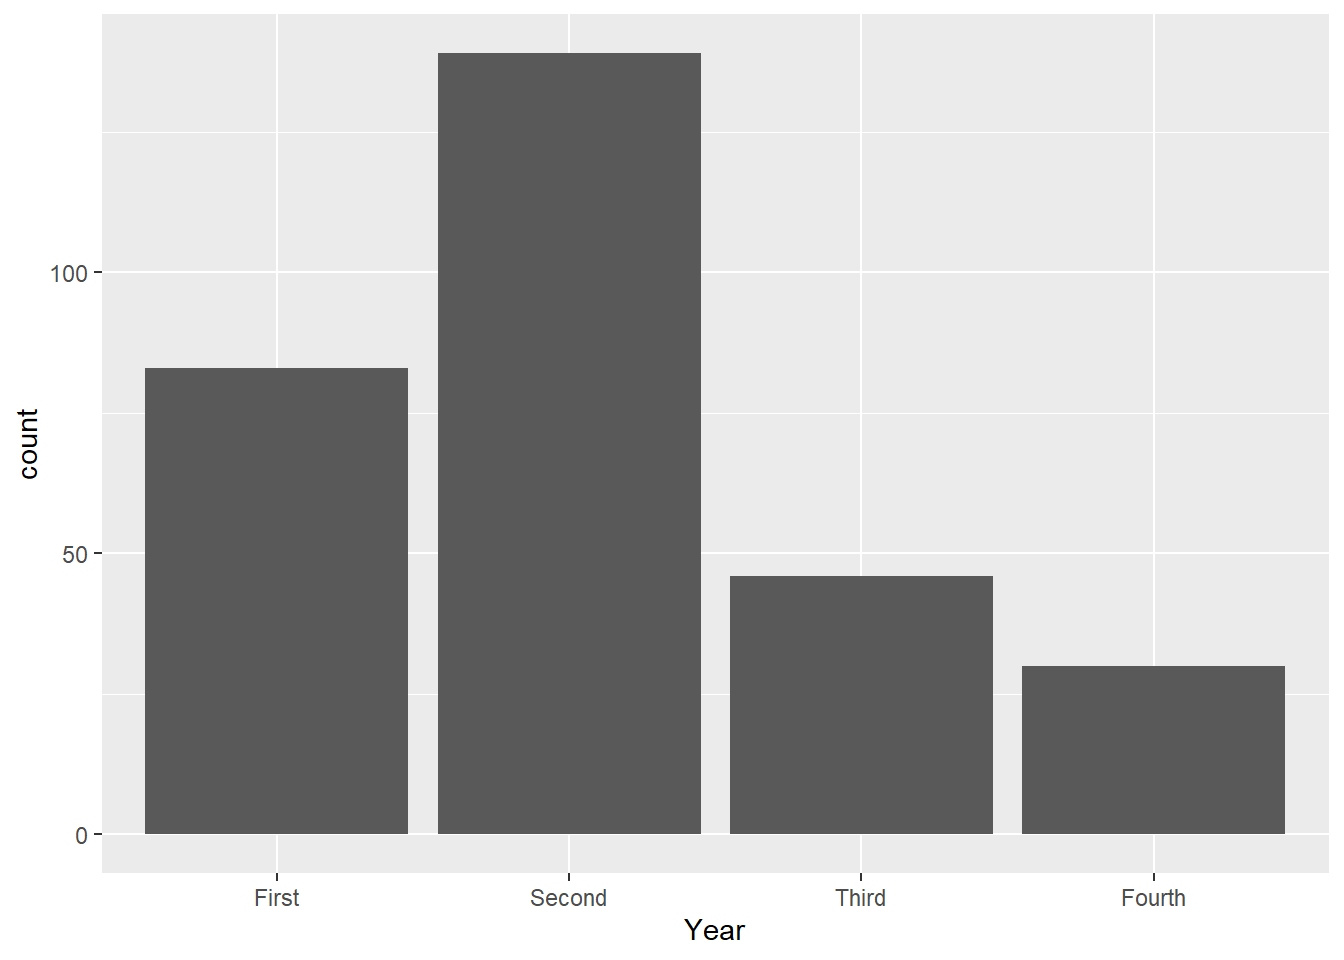
\includegraphics{bookdown-demo_files/figure-latex/unnamed-chunk-69-1.pdf}

We can read the number of students who are first, second, third, and fourth years by reading off the corresponding value on the vertical axis.

From these two lines we code, we can see the basic structure of creating data visualizations with the \texttt{ggplot()} function:

\begin{enumerate}
\def\labelenumi{\arabic{enumi}.}
\item
  Use the \texttt{ggplot()} function, and supply the name of the data frame, and the x- and/or y- variables via the aes() function. End this line with a \texttt{+} operator, and then press enter.
\item
  In the next line, specify the type of graph we want to create (called \texttt{geoms}). For a bar chart, type \texttt{geom\_bar()}.
\end{enumerate}

Some describe these lines of code as two layers of code. These two layers must be supplied for all data visualizations with \texttt{ggplot()}.

Additional optional layers can be added (these usually deal with the details of the visuals). Suppose we want to change the orientation of this bar chart, we can add an optional line, or layer:

\begin{Shaded}
\begin{Highlighting}[]
\FunctionTok{ggplot}\NormalTok{(Data, }\FunctionTok{aes}\NormalTok{(}\AttributeTok{x=}\NormalTok{Year))}\SpecialCharTok{+}
  \FunctionTok{geom\_bar}\NormalTok{()}\SpecialCharTok{+}
  \FunctionTok{coord\_flip}\NormalTok{()}
\end{Highlighting}
\end{Shaded}

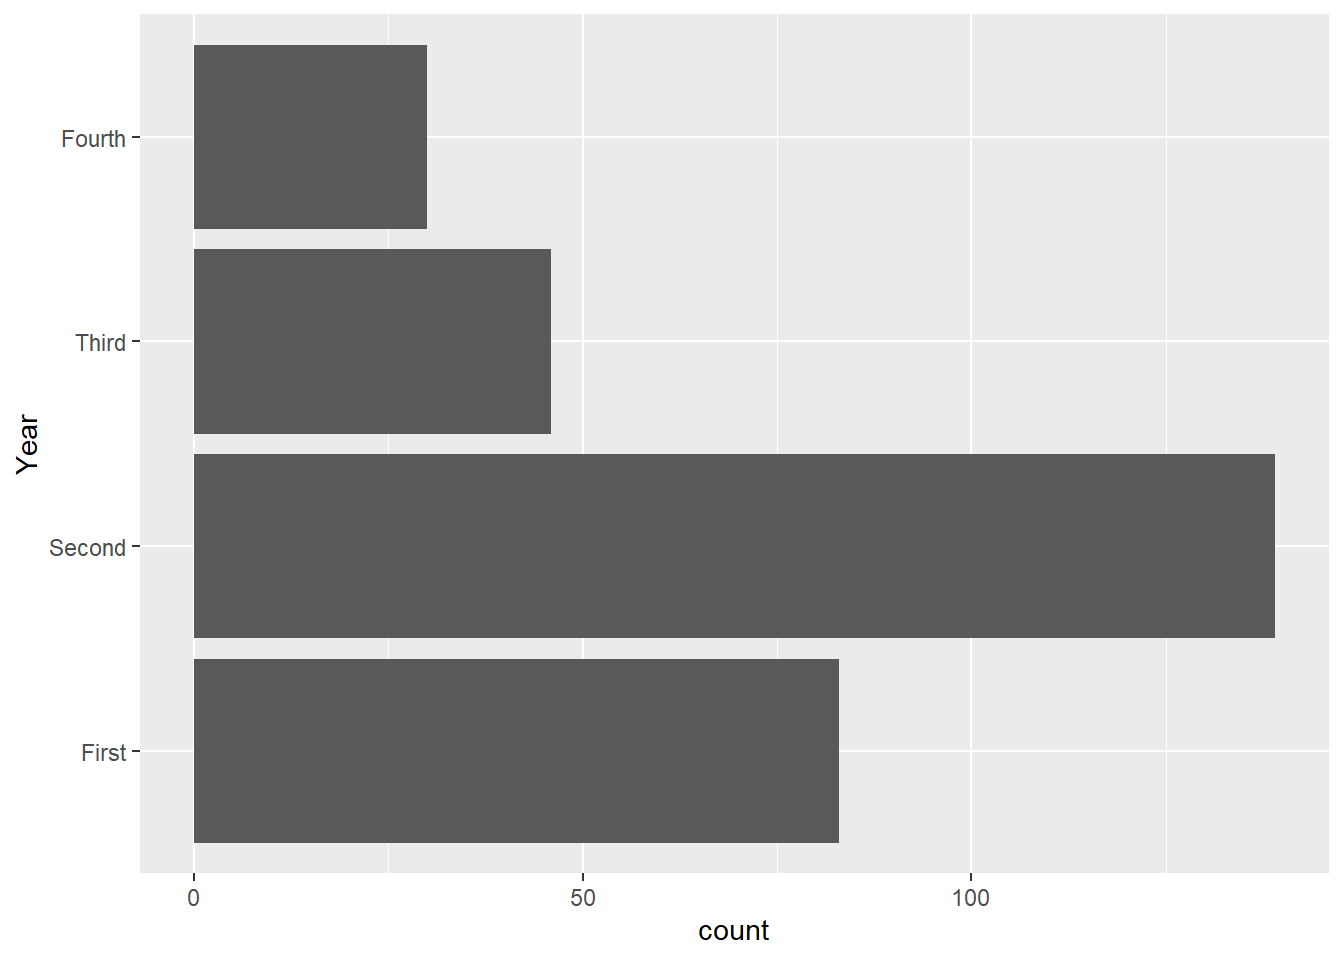
\includegraphics{bookdown-demo_files/figure-latex/unnamed-chunk-70-1.pdf}

It is recommended that each layer is typed on a line below the previous layer. A \texttt{+} sign is used at the end of each layer to add another layer below.

To change the color of the bars:

\begin{Shaded}
\begin{Highlighting}[]
\FunctionTok{ggplot}\NormalTok{(Data, }\FunctionTok{aes}\NormalTok{(}\AttributeTok{x=}\NormalTok{Year))}\SpecialCharTok{+}
  \FunctionTok{geom\_bar}\NormalTok{(}\AttributeTok{fill=}\StringTok{"blue"}\NormalTok{)}
\end{Highlighting}
\end{Shaded}

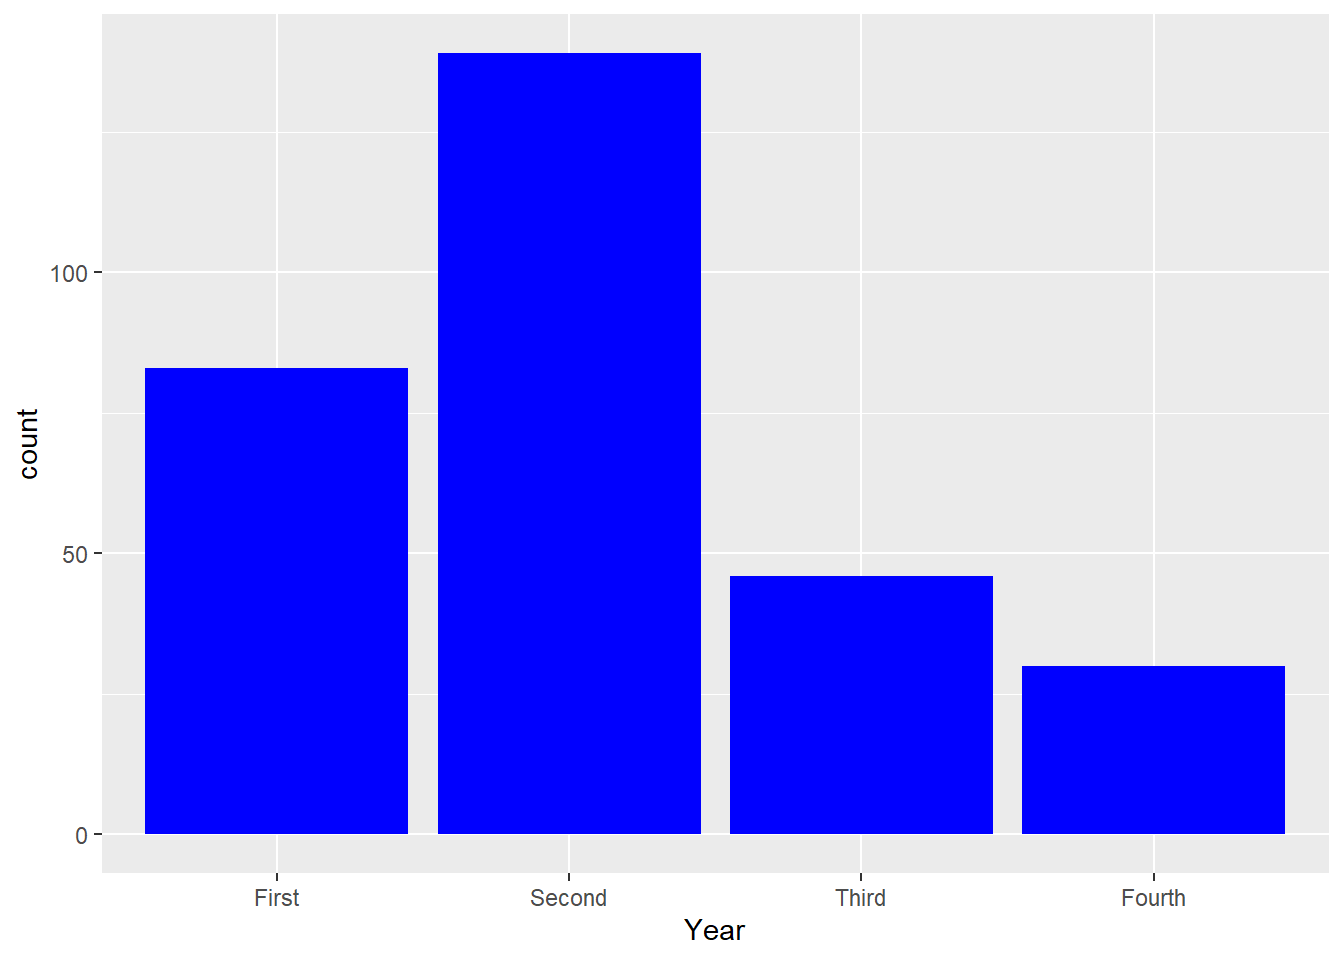
\includegraphics{bookdown-demo_files/figure-latex/unnamed-chunk-71-1.pdf}

To have a different color to outline the bars:

\begin{Shaded}
\begin{Highlighting}[]
\FunctionTok{ggplot}\NormalTok{(Data, }\FunctionTok{aes}\NormalTok{(}\AttributeTok{x=}\NormalTok{Year))}\SpecialCharTok{+}
  \FunctionTok{geom\_bar}\NormalTok{(}\AttributeTok{fill=}\StringTok{"blue"}\NormalTok{,}\AttributeTok{color=}\StringTok{"orange"}\NormalTok{)}
\end{Highlighting}
\end{Shaded}

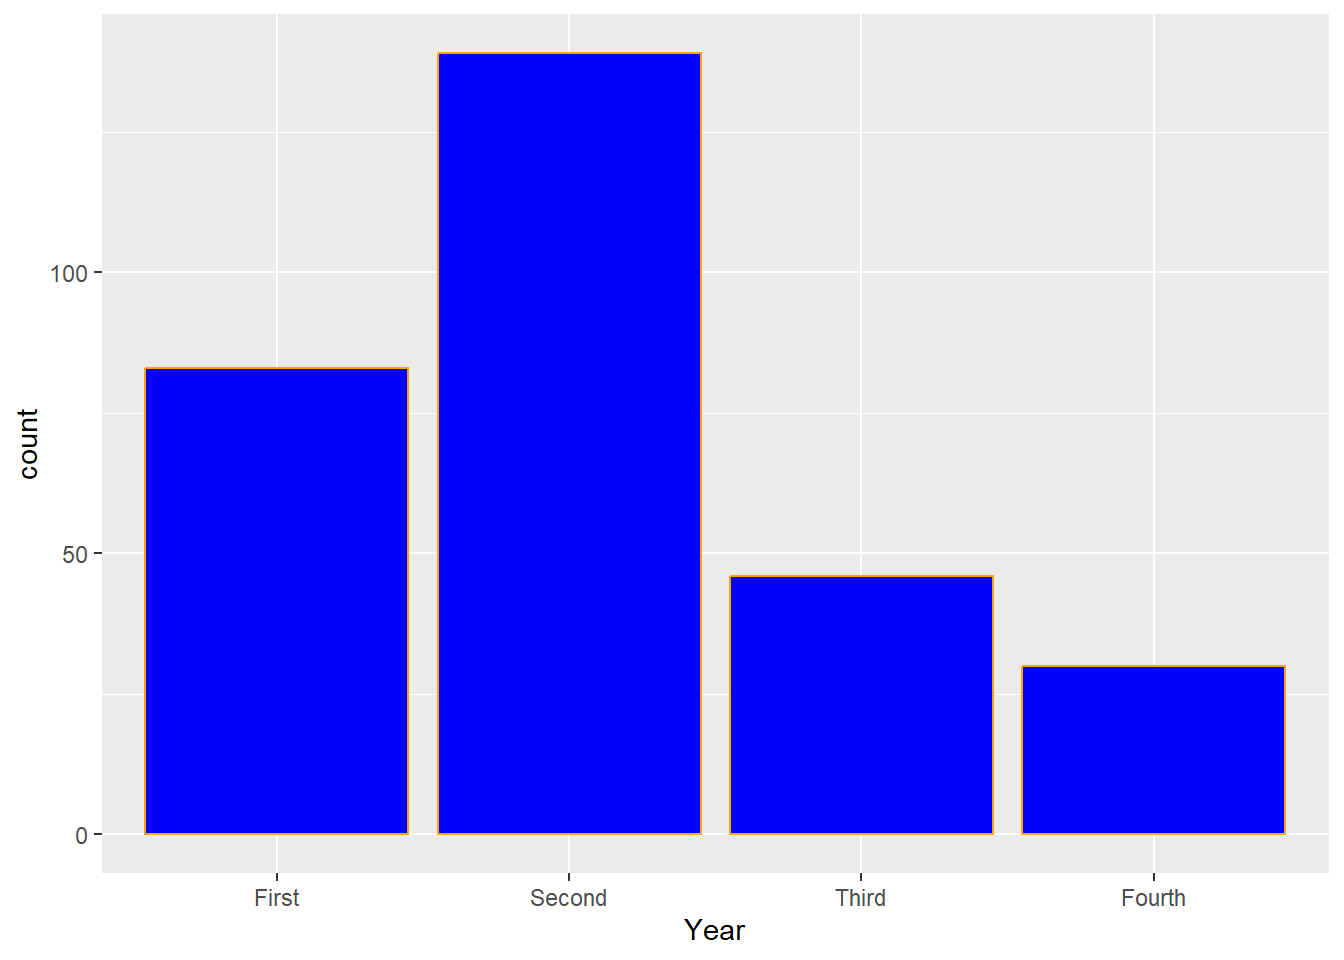
\includegraphics{bookdown-demo_files/figure-latex/unnamed-chunk-72-1.pdf}

\hypertarget{customize-title-and-labels-of-axes-in-bar-charts}{%
\subsubsection{Customize title and labels of axes in bar charts}\label{customize-title-and-labels-of-axes-in-bar-charts}}

To change the orientation of the labels on the horizontal axis, we add an extra layer called \texttt{theme}. This will be useful when we have many classes and/or labels with long names.

To rotate the labels on the horizontal by 90 degrees:

\begin{Shaded}
\begin{Highlighting}[]
\FunctionTok{ggplot}\NormalTok{(Data, }\FunctionTok{aes}\NormalTok{(}\AttributeTok{x=}\NormalTok{Year))}\SpecialCharTok{+}
  \FunctionTok{geom\_bar}\NormalTok{()}\SpecialCharTok{+}
  \FunctionTok{theme}\NormalTok{(}\AttributeTok{axis.text.x =} \FunctionTok{element\_text}\NormalTok{(}\AttributeTok{angle =} \DecValTok{90}\NormalTok{))}
\end{Highlighting}
\end{Shaded}

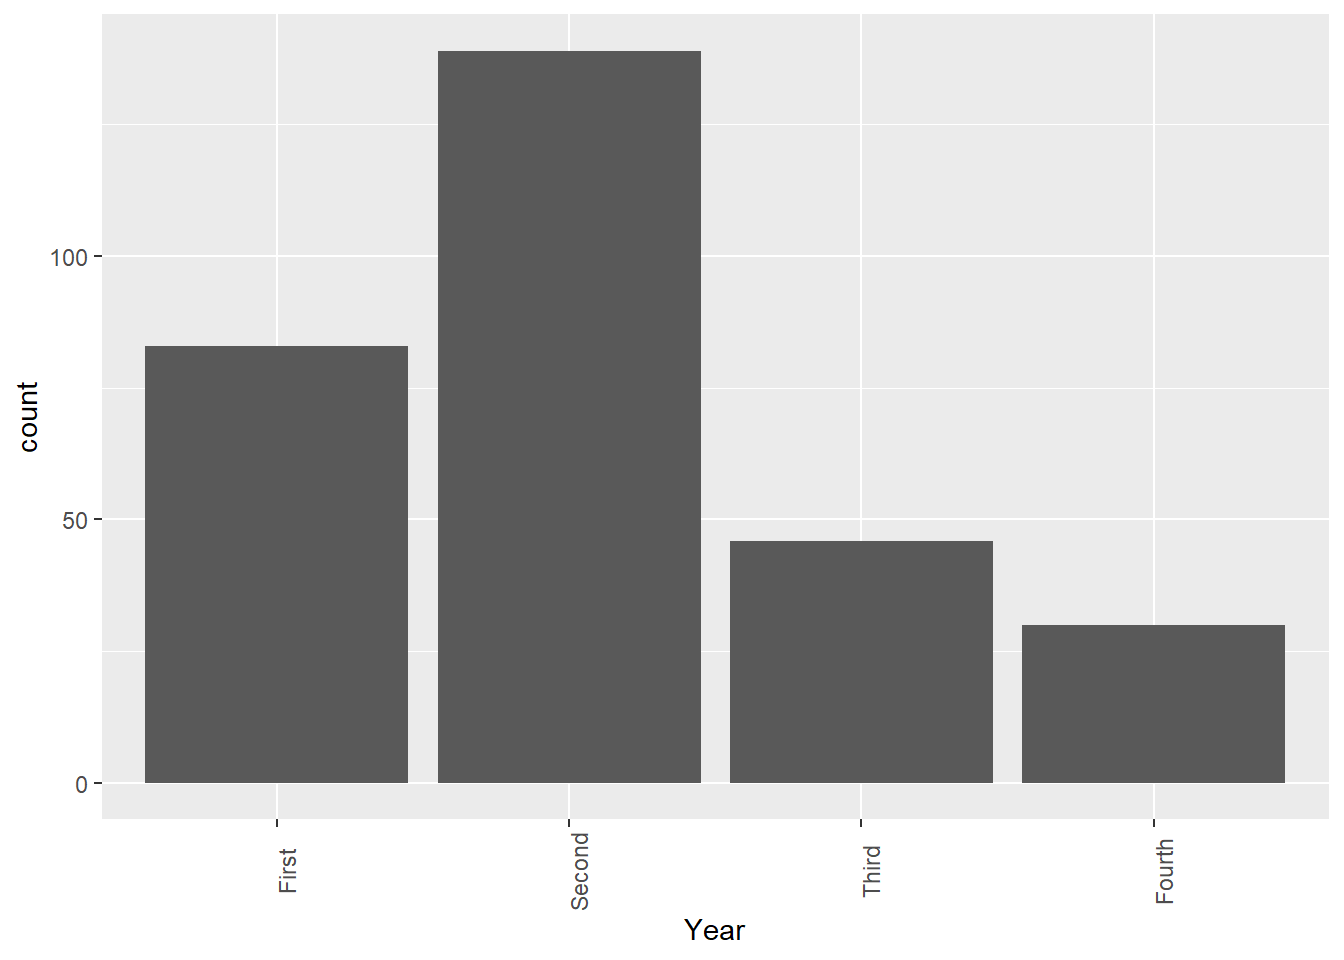
\includegraphics{bookdown-demo_files/figure-latex/unnamed-chunk-73-1.pdf}

As we create more visualizations, it is good practice to give short but meaningful and descriptive names for each axis and provide a title. We can change the labels of the x- and y- axes, as well as add a title for the bar chart by adding another layer called \texttt{labs}:

\begin{Shaded}
\begin{Highlighting}[]
\FunctionTok{ggplot}\NormalTok{(Data, }\FunctionTok{aes}\NormalTok{(}\AttributeTok{x=}\NormalTok{Year))}\SpecialCharTok{+}
  \FunctionTok{geom\_bar}\NormalTok{()}\SpecialCharTok{+}
  \FunctionTok{theme}\NormalTok{(}\AttributeTok{axis.text.x =} \FunctionTok{element\_text}\NormalTok{(}\AttributeTok{angle =} \DecValTok{90}\NormalTok{))}\SpecialCharTok{+}
  \FunctionTok{labs}\NormalTok{(}\AttributeTok{x=}\StringTok{"Year"}\NormalTok{, }\AttributeTok{y=}\StringTok{"Number of Students"}\NormalTok{, }\AttributeTok{title=}\StringTok{"Dist of Years"}\NormalTok{)}
\end{Highlighting}
\end{Shaded}

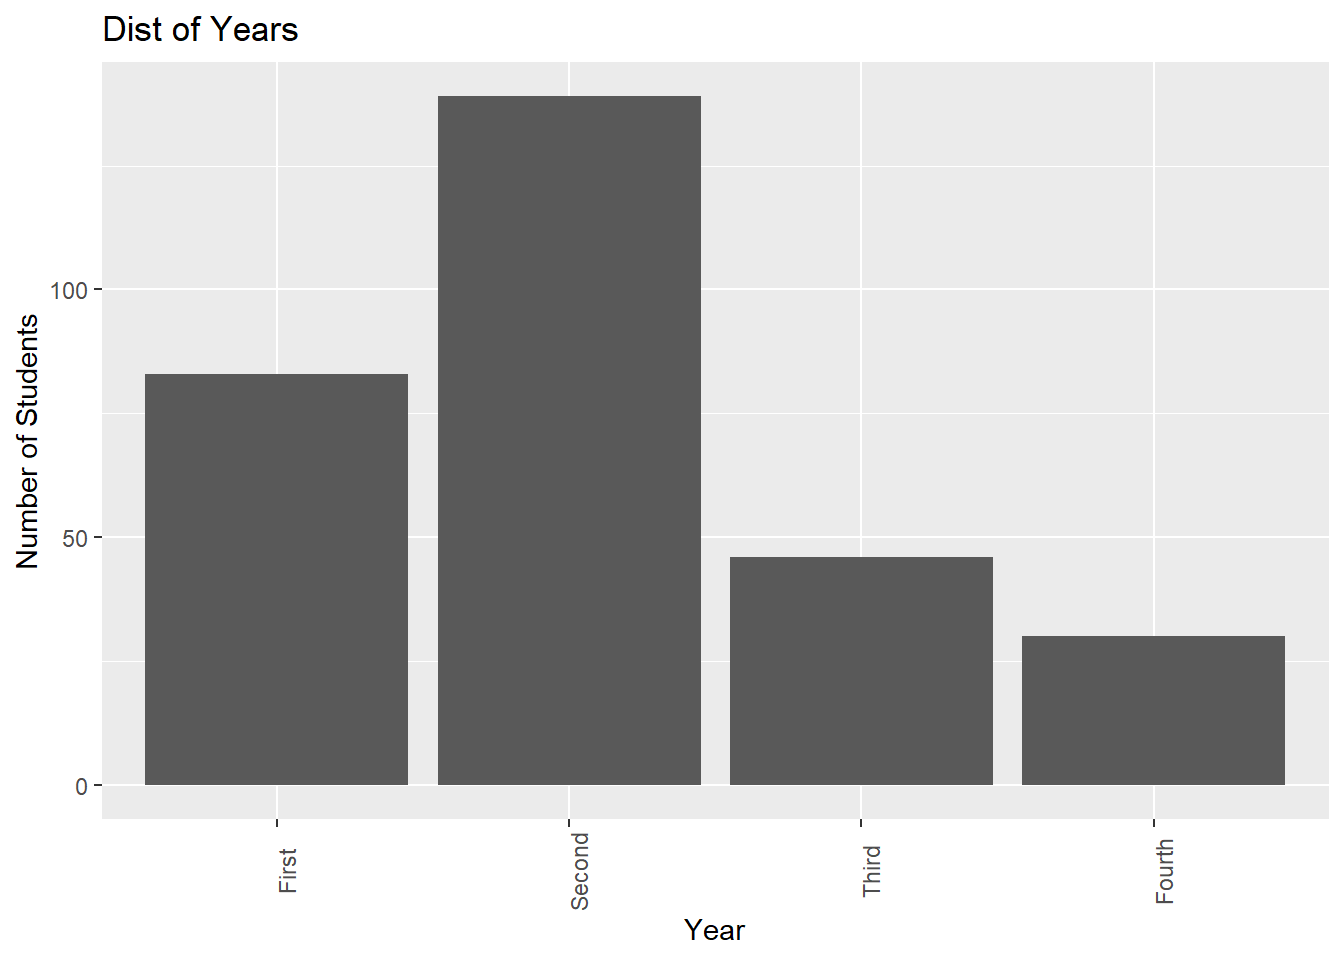
\includegraphics{bookdown-demo_files/figure-latex/unnamed-chunk-74-1.pdf}

We can also adjust the position of the title, for example, center-justify it via \texttt{theme}:

\begin{Shaded}
\begin{Highlighting}[]
\FunctionTok{ggplot}\NormalTok{(Data, }\FunctionTok{aes}\NormalTok{(}\AttributeTok{x=}\NormalTok{Year))}\SpecialCharTok{+}
  \FunctionTok{geom\_bar}\NormalTok{()}\SpecialCharTok{+}
  \FunctionTok{theme}\NormalTok{(}\AttributeTok{axis.text.x =} \FunctionTok{element\_text}\NormalTok{(}\AttributeTok{angle =} \DecValTok{90}\NormalTok{), }
        \AttributeTok{plot.title =} \FunctionTok{element\_text}\NormalTok{(}\AttributeTok{hjust =} \FloatTok{0.5}\NormalTok{))}\SpecialCharTok{+}
  \FunctionTok{labs}\NormalTok{(}\AttributeTok{x=}\StringTok{"Year"}\NormalTok{, }\AttributeTok{y=}\StringTok{"Number of Students"}\NormalTok{, }\AttributeTok{title=}\StringTok{"Dist of Years"}\NormalTok{)}
\end{Highlighting}
\end{Shaded}

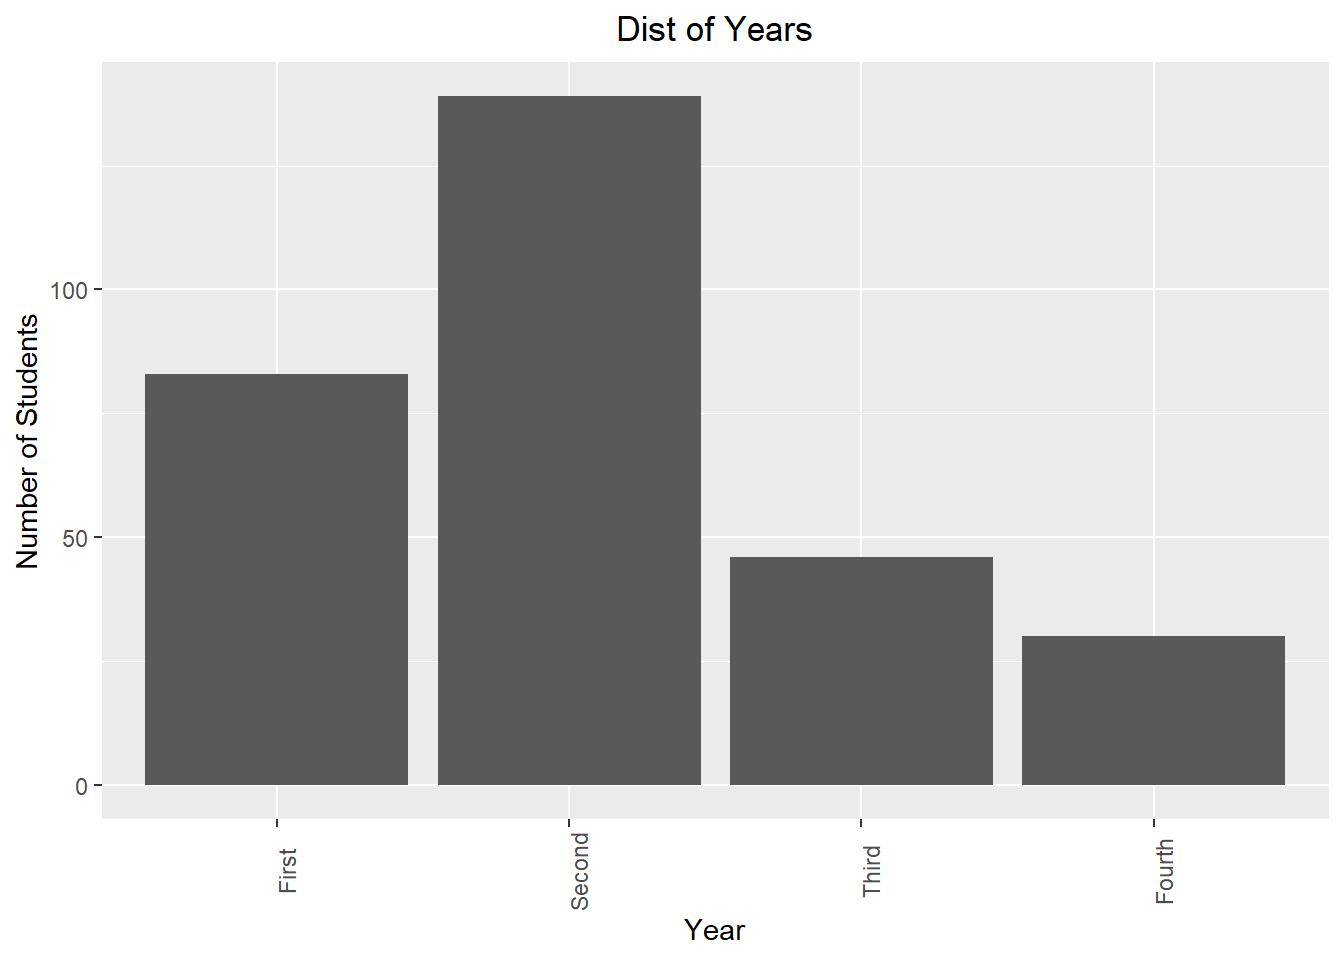
\includegraphics{bookdown-demo_files/figure-latex/unnamed-chunk-75-1.pdf}

\hypertarget{create-a-bar-chart-using-proportions}{%
\subsubsection{Create a bar chart using proportions}\label{create-a-bar-chart-using-proportions}}

Suppose we want to create a bar chart where the y-axis displays the proportions, rather than the counts of each level. There are a few steps to produce such a bar chart. First, we create a new dataframe, where each row represents a year, and we add the proportion of each year into a new column:

\begin{Shaded}
\begin{Highlighting}[]
\NormalTok{newData}\OtherTok{\textless{}{-}}\NormalTok{Data}\SpecialCharTok{\%\textgreater{}\%}
  \FunctionTok{group\_by}\NormalTok{(Year)}\SpecialCharTok{\%\textgreater{}\%}
  \FunctionTok{summarize}\NormalTok{(}\AttributeTok{Counts=}\FunctionTok{n}\NormalTok{())}\SpecialCharTok{\%\textgreater{}\%}
  \FunctionTok{mutate}\NormalTok{(}\AttributeTok{Percent=}\NormalTok{Counts}\SpecialCharTok{/}\FunctionTok{nrow}\NormalTok{(Data))}
\end{Highlighting}
\end{Shaded}

The code above does the following:

\begin{enumerate}
\def\labelenumi{\arabic{enumi}.}
\tightlist
\item
  Creates a new data frame called \texttt{newData} by taking the data frame called \texttt{Data},
\item
  and then groups the observations by \texttt{Year},
\item
  and then counts the number of observations in each \texttt{Year} and stores these values in a vector called \texttt{Counts},
\item
  and then creates a new vector called \texttt{Percent} by using the mathematical operations as specified in \texttt{mutate()}. \texttt{Percent} is added to \texttt{newData}.
\end{enumerate}

We can take a look at the contents of \texttt{newData}:

\begin{Shaded}
\begin{Highlighting}[]
\NormalTok{newData}
\end{Highlighting}
\end{Shaded}

\begin{verbatim}
## # A tibble: 4 x 3
##   Year   Counts Percent
##   <fct>   <int>   <dbl>
## 1 First      83   0.279
## 2 Second    139   0.466
## 3 Third      46   0.154
## 4 Fourth     30   0.101
\end{verbatim}

To create a bar chart using proportions:

\begin{Shaded}
\begin{Highlighting}[]
\FunctionTok{ggplot}\NormalTok{(newData, }\FunctionTok{aes}\NormalTok{(}\AttributeTok{x=}\NormalTok{Year, }\AttributeTok{y=}\NormalTok{Percent))}\SpecialCharTok{+}
  \FunctionTok{geom\_bar}\NormalTok{(}\AttributeTok{stat=}\StringTok{"identity"}\NormalTok{)}\SpecialCharTok{+}
  \FunctionTok{theme}\NormalTok{(}\AttributeTok{axis.text.x =} \FunctionTok{element\_text}\NormalTok{(}\AttributeTok{angle =} \DecValTok{90}\NormalTok{), }
        \AttributeTok{plot.title =} \FunctionTok{element\_text}\NormalTok{(}\AttributeTok{hjust =} \FloatTok{0.5}\NormalTok{))}\SpecialCharTok{+}
  \FunctionTok{labs}\NormalTok{(}\AttributeTok{x=}\StringTok{"Year"}\NormalTok{, }\AttributeTok{y=}\StringTok{"Percent of Students"}\NormalTok{, }\AttributeTok{title=}\StringTok{"Dist of Years"}\NormalTok{)}
\end{Highlighting}
\end{Shaded}

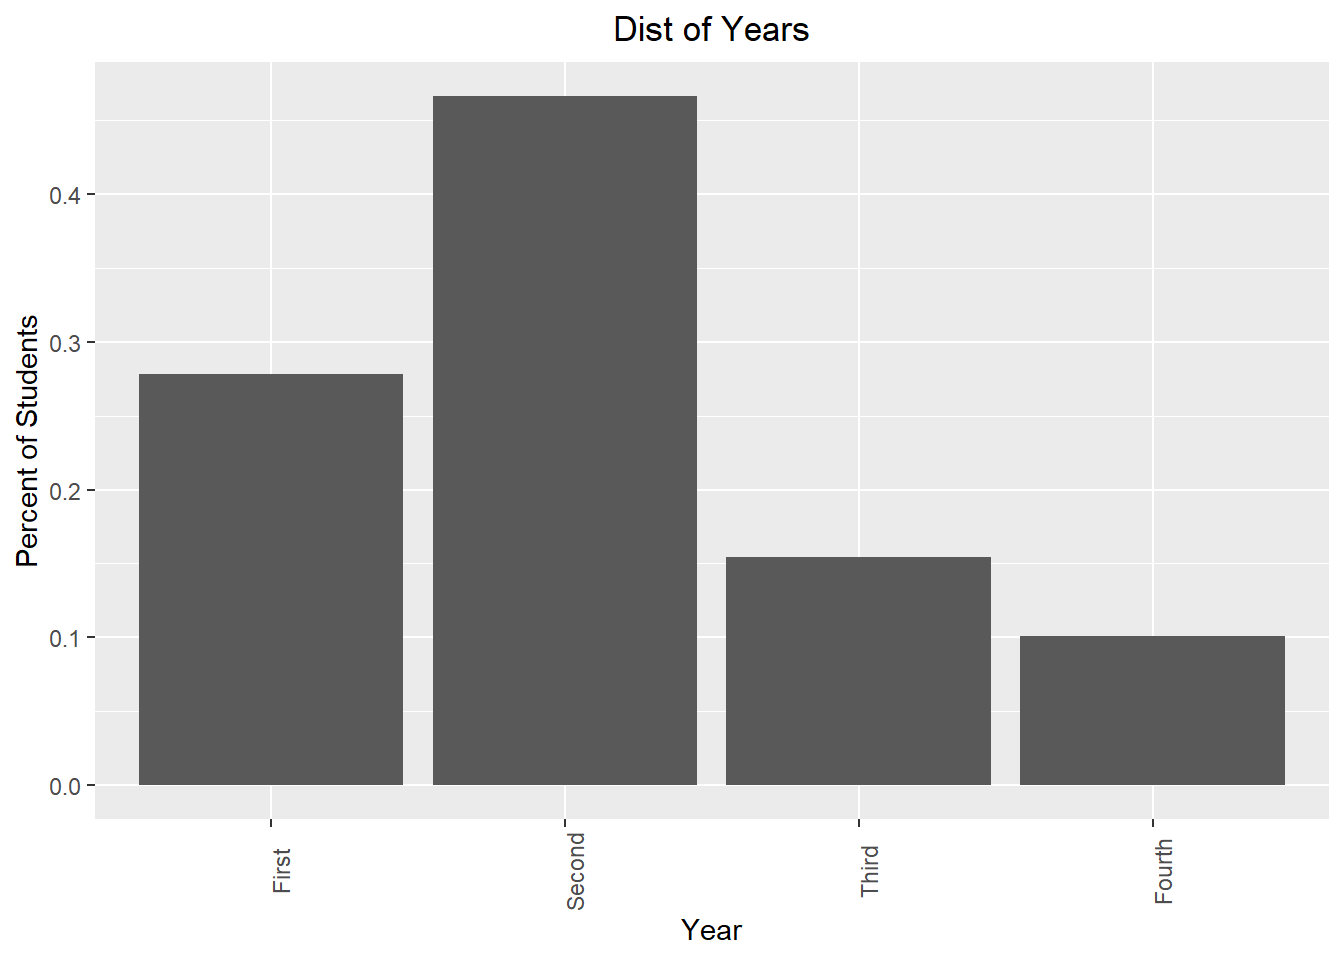
\includegraphics{bookdown-demo_files/figure-latex/unnamed-chunk-78-1.pdf}

Note the following:

\begin{enumerate}
\def\labelenumi{\arabic{enumi}.}
\tightlist
\item
  In the first layer, we use \texttt{newData} instead of the old data frame. In \texttt{aes()}, we specified a y-variable, which we want to be \texttt{Percent}.
\item
  In the second layer, we specified \texttt{stat="identity"} inside \texttt{geom\_bar()}.
\end{enumerate}

\hypertarget{visualizations-with-a-single-quantitative-variable}{%
\section{Visualizations with a Single Quantitative Variable}\label{visualizations-with-a-single-quantitative-variable}}

\hypertarget{number-summary}{%
\subsection{5 number summary}\label{number-summary}}

The \texttt{summary()} function, when applied to a quantitative variable, produces the 5 number summary: the minimum, the first quartile (25th percentile), the median (50th percentile), the third quartile (75th percentile), and the maximum, as well as the mean. For example, to obtain the 5 number summary of the ages of these students:

\begin{Shaded}
\begin{Highlighting}[]
\FunctionTok{summary}\NormalTok{(Data}\SpecialCharTok{$}\NormalTok{Age)}
\end{Highlighting}
\end{Shaded}

\begin{verbatim}
##    Min. 1st Qu.  Median    Mean 3rd Qu.    Max. 
##   18.00   19.00   19.00   19.57   20.00   51.00
\end{verbatim}

The average age of the observations in this dataset is 19.57 years old. Notice the first quartile and the median are both 19 years old, that means at least a quarter of the observations are 19 years old. Also note the maximum of 51 years old, so we have a student who is quite a lot older than the rest.

\hypertarget{boxplots}{%
\subsection{Boxplots}\label{boxplots}}

A boxplot is a graphical representation of the 5 number summary. To create a generic boxplot, we have the following two lines of code when using the \texttt{ggplot()} function:

\begin{Shaded}
\begin{Highlighting}[]
\FunctionTok{ggplot}\NormalTok{(Data, }\FunctionTok{aes}\NormalTok{(}\AttributeTok{y=}\NormalTok{Age))}\SpecialCharTok{+}
  \FunctionTok{geom\_boxplot}\NormalTok{()}
\end{Highlighting}
\end{Shaded}

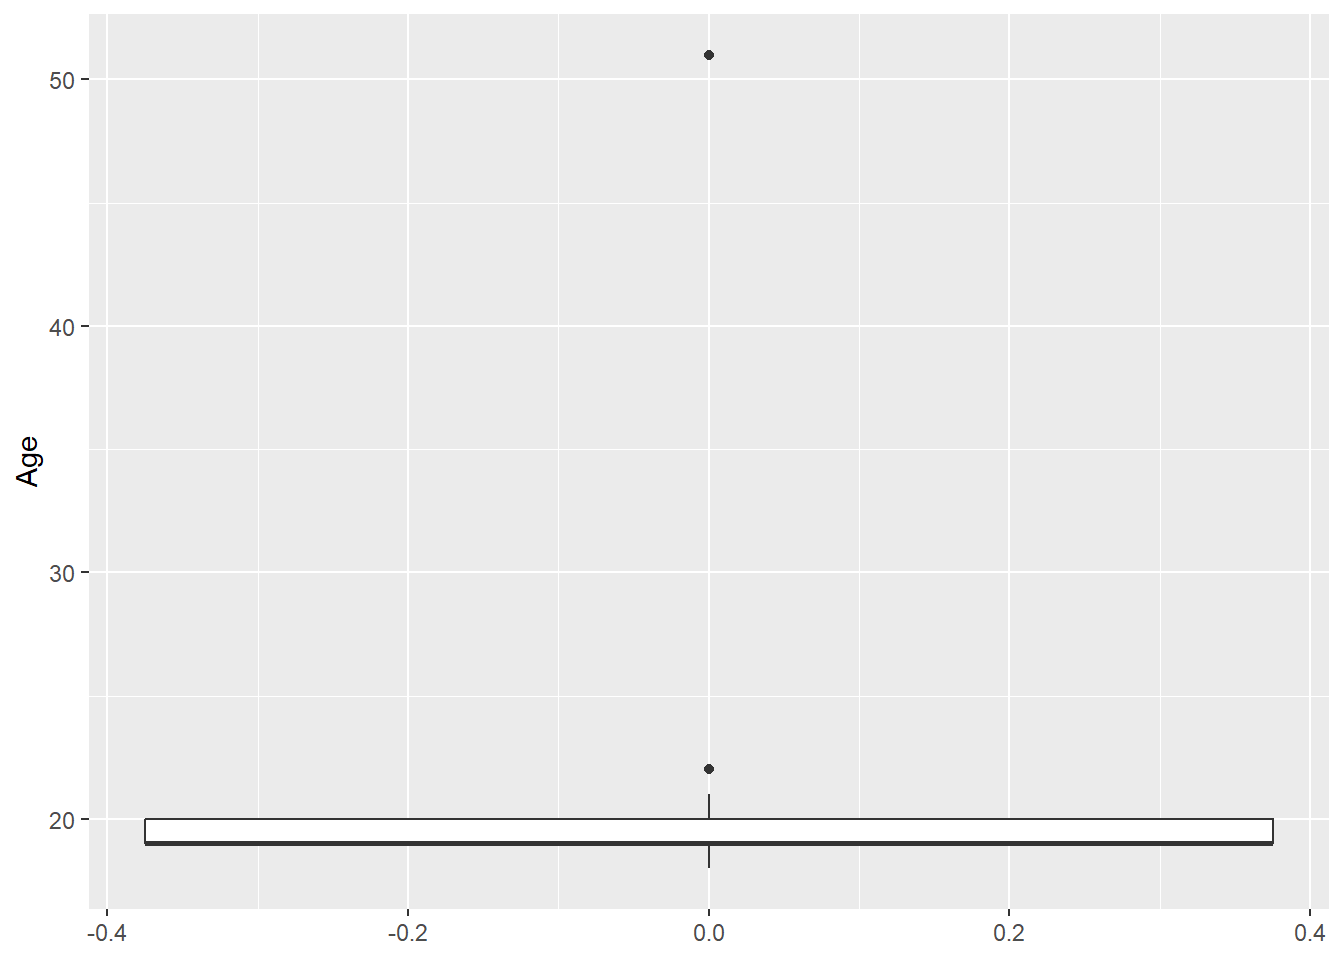
\includegraphics{bookdown-demo_files/figure-latex/unnamed-chunk-80-1.pdf}

Note we are still using the same structure when creating data visualizations with \texttt{ggplot()}:

\begin{enumerate}
\def\labelenumi{\arabic{enumi}.}
\item
  Use the \texttt{ggplot()} function, and supply the name of the data frame, and the x- and/or y- variables via the aes() function. End this line with a \texttt{+} operator, and then press enter.
\item
  In the next line, specify the type of graph we want to create (called \texttt{geoms}). For a boxplot, type \texttt{geom\_boxplot}.
\end{enumerate}

Notice there are outliers (observations that are a lot older or younger) that are denoted by the dots. One is the 51 year old, and 22 year olds are deemed to be outliers. The rule being used is the \(1.5 \times IQR\) rule.

Similar to bar charts, we can change the orientation of boxplots by adding an additional layer as before:

\begin{Shaded}
\begin{Highlighting}[]
\FunctionTok{ggplot}\NormalTok{(Data, }\FunctionTok{aes}\NormalTok{(}\AttributeTok{y=}\NormalTok{Age))}\SpecialCharTok{+}
  \FunctionTok{geom\_boxplot}\NormalTok{()}\SpecialCharTok{+}
  \FunctionTok{coord\_flip}\NormalTok{()}
\end{Highlighting}
\end{Shaded}

We can change the color of the box and the outliers similarly:

\begin{Shaded}
\begin{Highlighting}[]
\FunctionTok{ggplot}\NormalTok{(Data, }\FunctionTok{aes}\NormalTok{(}\AttributeTok{y=}\NormalTok{Age))}\SpecialCharTok{+}
  \FunctionTok{geom\_boxplot}\NormalTok{(}\AttributeTok{color=}\StringTok{"blue"}\NormalTok{, }\AttributeTok{outlier.color =} \StringTok{"orange"}\NormalTok{ )}
\end{Highlighting}
\end{Shaded}

\hypertarget{histograms}{%
\subsection{Histograms}\label{histograms}}

A histogram displays the number of observations within each bin on the x-axis:

\begin{Shaded}
\begin{Highlighting}[]
\FunctionTok{ggplot}\NormalTok{(Data,}\FunctionTok{aes}\NormalTok{(}\AttributeTok{x=}\NormalTok{Age))}\SpecialCharTok{+}
  \FunctionTok{geom\_histogram}\NormalTok{()}
\end{Highlighting}
\end{Shaded}

\begin{verbatim}
## `stat_bin()` using `bins = 30`. Pick better value with `binwidth`.
\end{verbatim}

Notice a warning message is displayed when creating a basic histogram. To fix this, we use the binwidth argument within \texttt{geom\_histogram}. We try \texttt{binwidth=1} for now, which means the width of the bin is 1 unit:

\begin{Shaded}
\begin{Highlighting}[]
\FunctionTok{ggplot}\NormalTok{(Data,}\FunctionTok{aes}\NormalTok{(}\AttributeTok{x=}\NormalTok{Age))}\SpecialCharTok{+}
  \FunctionTok{geom\_histogram}\NormalTok{(}\AttributeTok{binwidth =} \DecValTok{1}\NormalTok{,}\AttributeTok{fill=}\StringTok{"blue"}\NormalTok{,}\AttributeTok{color=}\StringTok{"orange"}\NormalTok{)}
\end{Highlighting}
\end{Shaded}

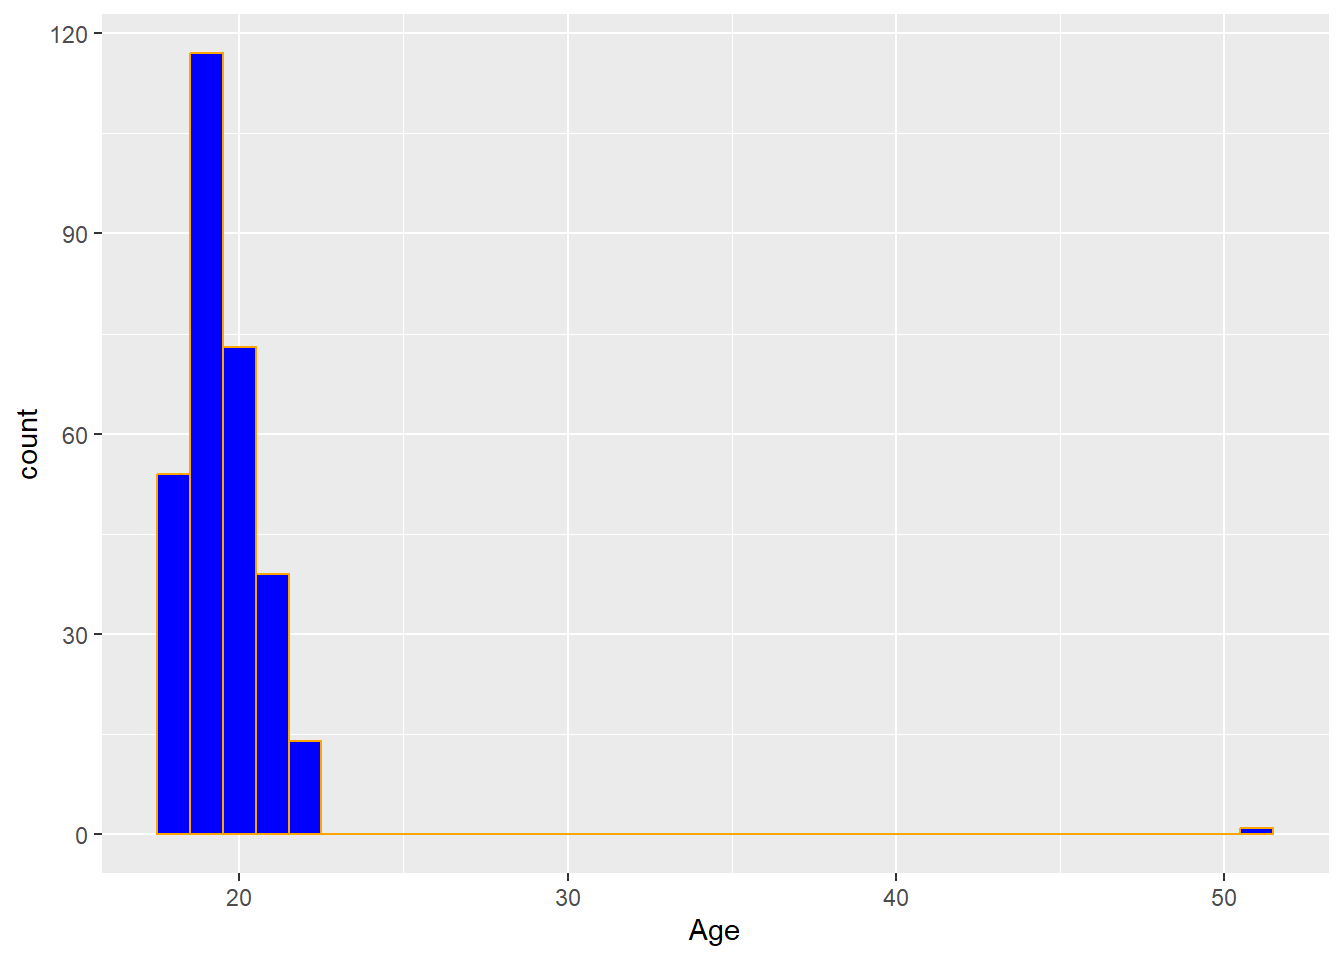
\includegraphics{bookdown-demo_files/figure-latex/unnamed-chunk-84-1.pdf}

The ages of the students are mostly young, with 19 and 20 years olds being the most commonly occuring.

A well-known drawback of histograms is that the width of the bins can drastically affect the visual. For example, suppose we change the binwidth to 2:

\begin{Shaded}
\begin{Highlighting}[]
\FunctionTok{ggplot}\NormalTok{(Data,}\FunctionTok{aes}\NormalTok{(}\AttributeTok{x=}\NormalTok{Age))}\SpecialCharTok{+}
  \FunctionTok{geom\_histogram}\NormalTok{(}\AttributeTok{binwidth =} \DecValTok{2}\NormalTok{,}\AttributeTok{fill=}\StringTok{"blue"}\NormalTok{,}\AttributeTok{color=}\StringTok{"orange"}\NormalTok{)}
\end{Highlighting}
\end{Shaded}

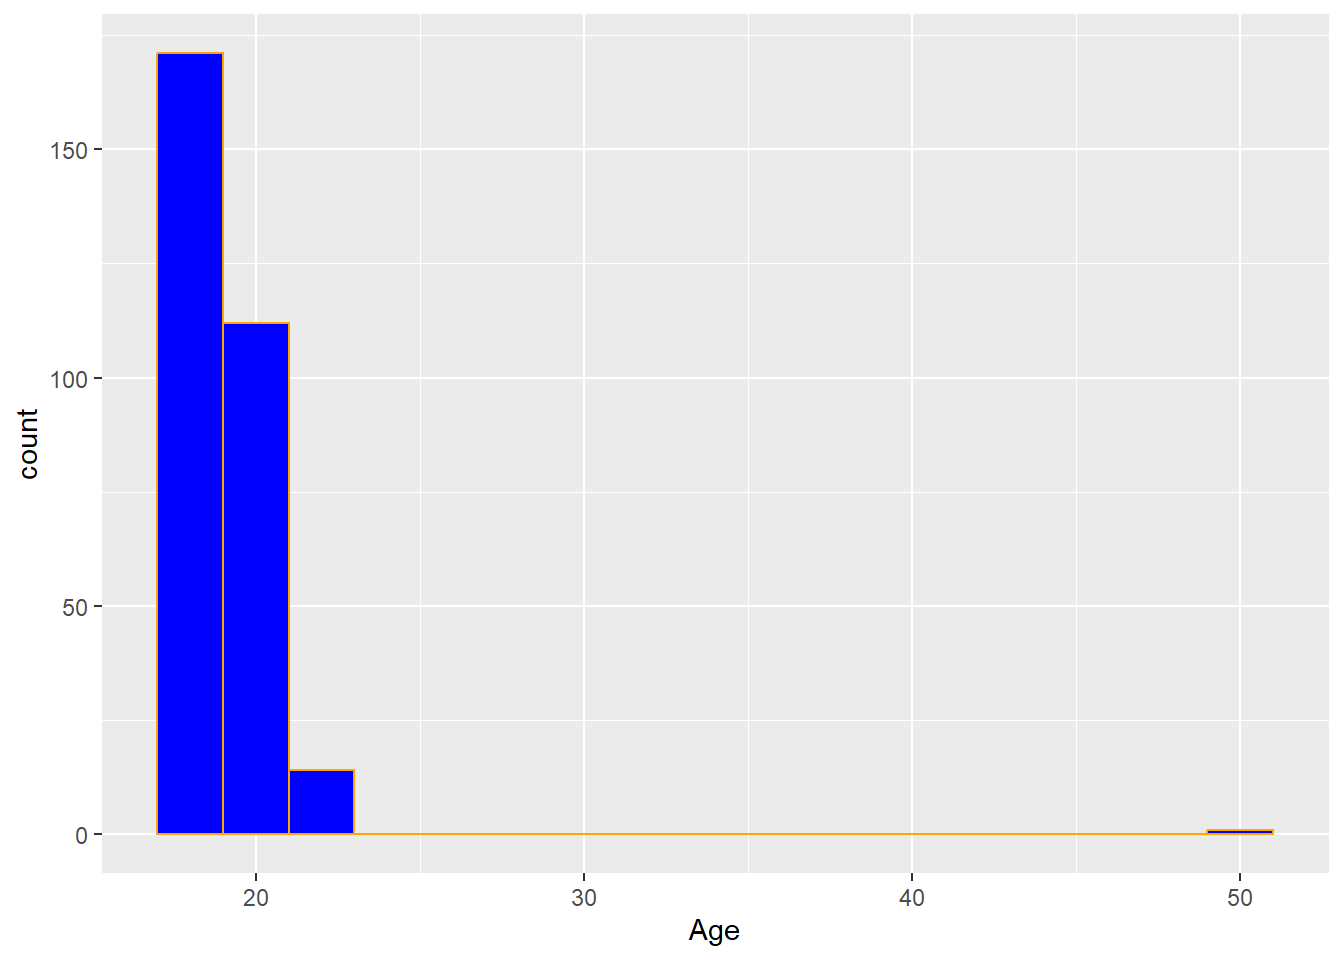
\includegraphics{bookdown-demo_files/figure-latex/unnamed-chunk-85-1.pdf}

Each bar now contains two ages: the first bar contains the 18 and 19 year olds. Notice how the shape has been changed a little bit from the previous histogram with a different binwidth?

\hypertarget{density-plots}{%
\subsection{Density plots}\label{density-plots}}

Density plots are a variation of histograms, where the plot attempts to use a smooth mathematical function to approximate the shape of the histogram, and is unaffected by binwidth:

\begin{Shaded}
\begin{Highlighting}[]
\FunctionTok{ggplot}\NormalTok{(Data,}\FunctionTok{aes}\NormalTok{(}\AttributeTok{x=}\NormalTok{Age))}\SpecialCharTok{+}
  \FunctionTok{geom\_density}\NormalTok{()}
\end{Highlighting}
\end{Shaded}

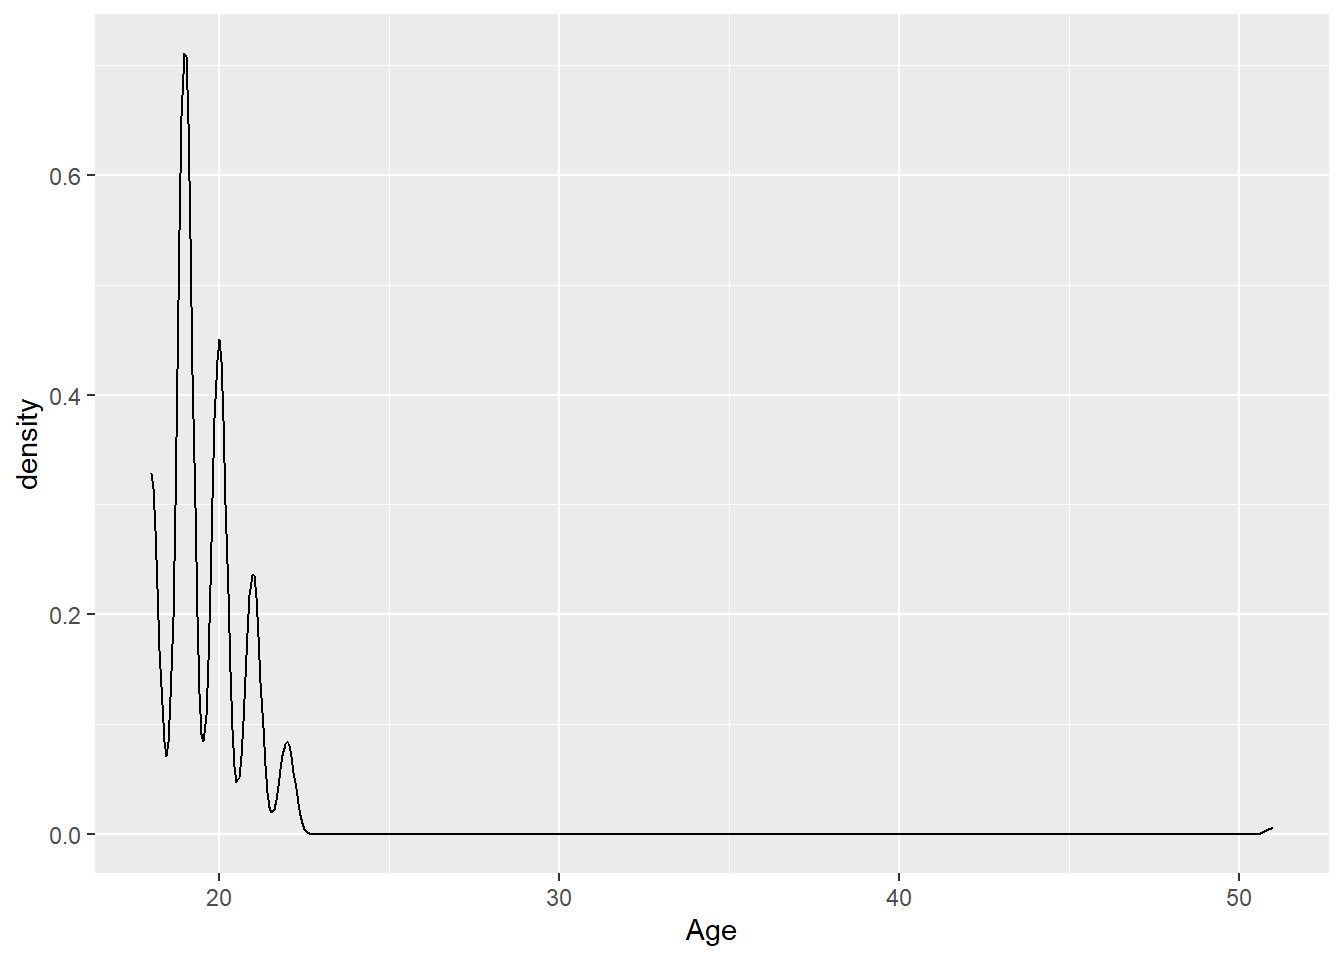
\includegraphics{bookdown-demo_files/figure-latex/unnamed-chunk-86-1.pdf}

We can see that 19 and 20 year olds are the most common ages in this data. Be careful in interpreting the values on the veritical axis: these do not represent proportions. A characteristic of density plots is that the area under the plot is always one.

\hypertarget{bivariate-visualizations}{%
\section{Bivariate Visualizations}\label{bivariate-visualizations}}

We will now look at visualizations we can create to explore the relationship between two variables. The term bivariate means that we are looking at two variables.

We will be using a new dataset as an example, so we clear the environment:

\begin{Shaded}
\begin{Highlighting}[]
\FunctionTok{rm}\NormalTok{(}\AttributeTok{list =} \FunctionTok{ls}\NormalTok{())}
\end{Highlighting}
\end{Shaded}

We will be using the dataset, \texttt{gapminder}, from the \texttt{gapminder} package. Install and load the \texttt{gapminder} package. Also load the \texttt{tidyverse} package (which automatically loads the \texttt{ggplot2} package):

\begin{Shaded}
\begin{Highlighting}[]
\FunctionTok{library}\NormalTok{(tidyverse)}
\FunctionTok{library}\NormalTok{(gapminder)}
\end{Highlighting}
\end{Shaded}

We can take a look at the \texttt{gapminder} dataset:

\begin{Shaded}
\begin{Highlighting}[]
\NormalTok{gapminder[}\DecValTok{1}\SpecialCharTok{:}\DecValTok{15}\NormalTok{,]}
\end{Highlighting}
\end{Shaded}

\begin{verbatim}
## # A tibble: 15 x 6
##    country     continent  year lifeExp      pop gdpPercap
##    <fct>       <fct>     <int>   <dbl>    <int>     <dbl>
##  1 Afghanistan Asia       1952    28.8  8425333      779.
##  2 Afghanistan Asia       1957    30.3  9240934      821.
##  3 Afghanistan Asia       1962    32.0 10267083      853.
##  4 Afghanistan Asia       1967    34.0 11537966      836.
##  5 Afghanistan Asia       1972    36.1 13079460      740.
##  6 Afghanistan Asia       1977    38.4 14880372      786.
##  7 Afghanistan Asia       1982    39.9 12881816      978.
##  8 Afghanistan Asia       1987    40.8 13867957      852.
##  9 Afghanistan Asia       1992    41.7 16317921      649.
## 10 Afghanistan Asia       1997    41.8 22227415      635.
## 11 Afghanistan Asia       2002    42.1 25268405      727.
## 12 Afghanistan Asia       2007    43.8 31889923      975.
## 13 Albania     Europe     1952    55.2  1282697     1601.
## 14 Albania     Europe     1957    59.3  1476505     1942.
## 15 Albania     Europe     1962    64.8  1728137     2313.
\end{verbatim}

Per the documentation, the variables are

\begin{enumerate}
\def\labelenumi{\arabic{enumi}.}
\tightlist
\item
  \texttt{country}
\item
  \texttt{continent}
\item
  \texttt{year}: from 1952 to 2007 in increments of 5 years
\item
  \texttt{lifeExp}: life expectancy at birth, in years
\item
  \texttt{pop}: population of country
\item
  \texttt{gdpPercap}: GDP per capita in US dollars, adjusted for inflation
\end{enumerate}

We notice that data are collected from each country across a number of different years: 1952 to 2007 in increments of five years. For this example, we will mainly focus on the data for the most recent year, 2007:

\begin{Shaded}
\begin{Highlighting}[]
\NormalTok{Data}\OtherTok{\textless{}{-}}\NormalTok{gapminder}\SpecialCharTok{\%\textgreater{}\%}
  \FunctionTok{filter}\NormalTok{(year}\SpecialCharTok{==}\DecValTok{2007}\NormalTok{)}
\end{Highlighting}
\end{Shaded}

The specific visuals to use will again depend on the type of variables we are using, whether they are categorical or quantitative.

\hypertarget{compare-quantitative-variable-across-categories}{%
\subsection{Compare quantitative variable across categories}\label{compare-quantitative-variable-across-categories}}

\hypertarget{side-by-side-boxplots}{%
\subsubsection{Side by side boxplots}\label{side-by-side-boxplots}}

Side by side boxplots are useful to compare a quantitative variable across different classes of a categorical variable. For example, we want to compare life expectancies across the different continents in the year 2007:

\begin{Shaded}
\begin{Highlighting}[]
\FunctionTok{ggplot}\NormalTok{(Data, }\FunctionTok{aes}\NormalTok{(}\AttributeTok{x=}\NormalTok{continent, }\AttributeTok{y=}\NormalTok{lifeExp))}\SpecialCharTok{+}
  \FunctionTok{geom\_boxplot}\NormalTok{(}\AttributeTok{fill=}\StringTok{"Blue"}\NormalTok{)}\SpecialCharTok{+}
  \FunctionTok{labs}\NormalTok{(}\AttributeTok{x=}\StringTok{"Continent"}\NormalTok{, }\AttributeTok{y=}\StringTok{"Life Exp"}\NormalTok{, }\AttributeTok{title=}\StringTok{"Dist of Life Expectancies by Continent"}\NormalTok{)}
\end{Highlighting}
\end{Shaded}

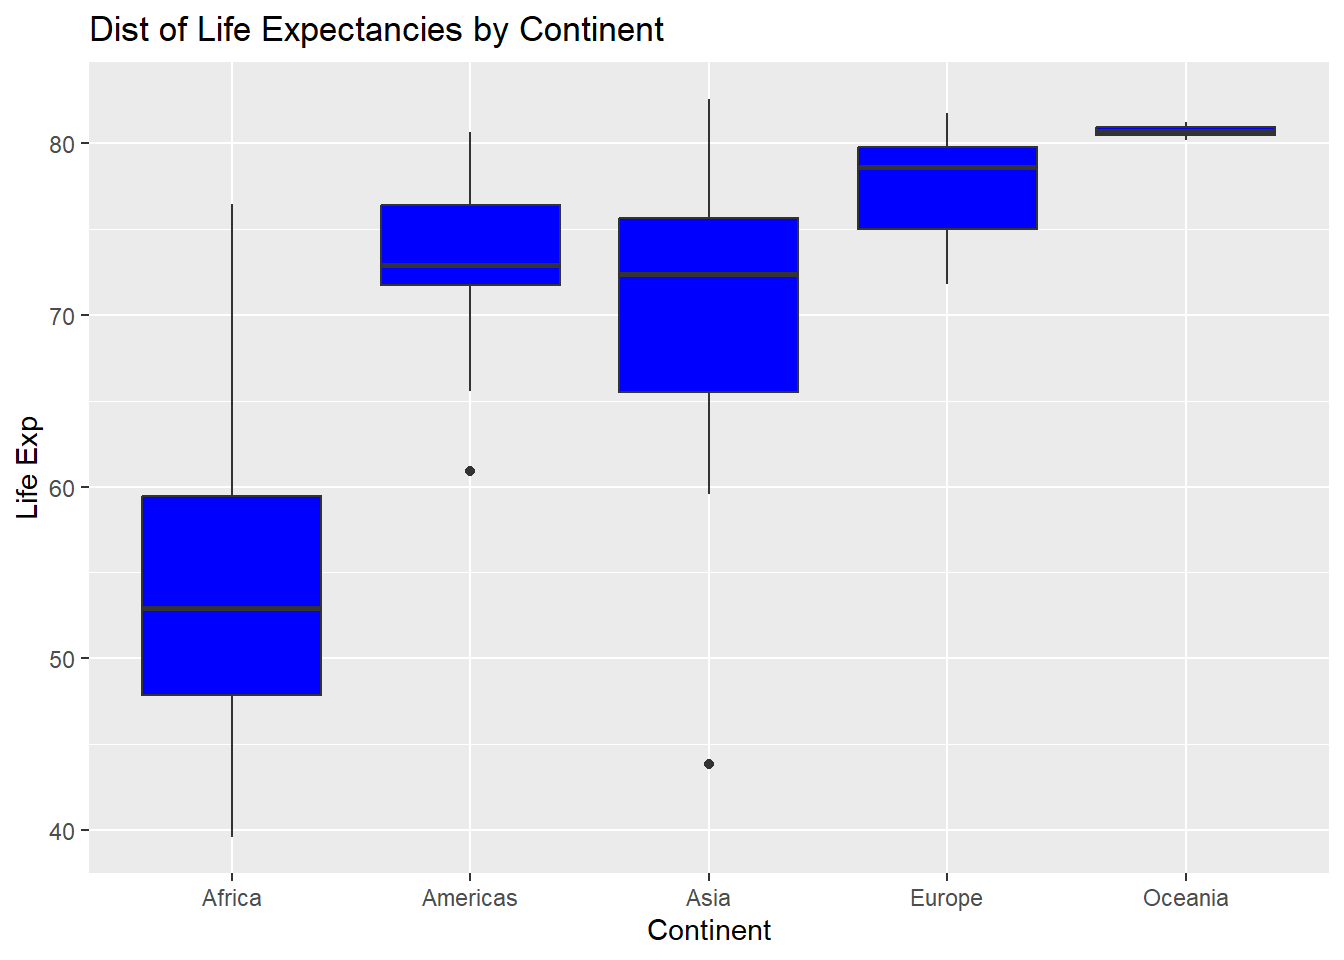
\includegraphics{bookdown-demo_files/figure-latex/unnamed-chunk-91-1.pdf}

Countries in the Oceania region have long life expectancies with little variation. Comparing the Americas and Asia, the median life expectancies are similar, but the spread is larger for Asia.

\hypertarget{violin-plots}{%
\subsubsection{Violin plots}\label{violin-plots}}

Violin plots are an alternative to boxplots. To create these plots to compare life expectancies across the different continents in the year 2007:

\begin{Shaded}
\begin{Highlighting}[]
\FunctionTok{ggplot}\NormalTok{(Data, }\FunctionTok{aes}\NormalTok{(}\AttributeTok{x=}\NormalTok{continent, }\AttributeTok{y=}\NormalTok{lifeExp))}\SpecialCharTok{+}
  \FunctionTok{geom\_violin}\NormalTok{()}\SpecialCharTok{+}
  \FunctionTok{labs}\NormalTok{(}\AttributeTok{x=}\StringTok{"Continent"}\NormalTok{, }\AttributeTok{y=}\StringTok{"Life Exp"}\NormalTok{, }\AttributeTok{title=}\StringTok{"Dist of Life Expectancies by Continent"}\NormalTok{)}
\end{Highlighting}
\end{Shaded}

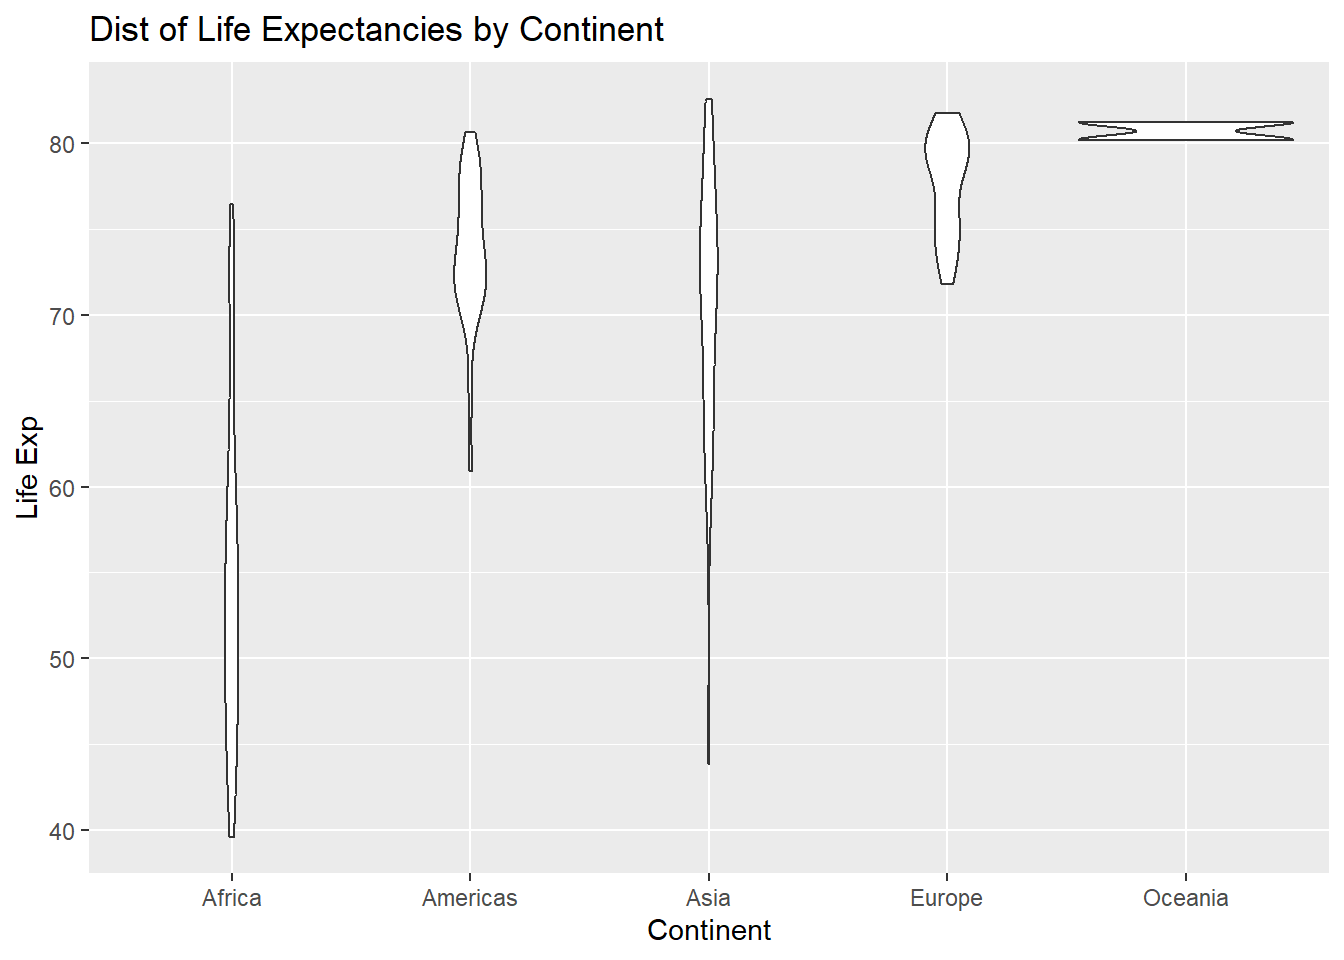
\includegraphics{bookdown-demo_files/figure-latex/unnamed-chunk-92-1.pdf}

The width of the violin informs us which values are more commonly occuring. For example, look at the violin for Europe. The violin is wider at higher life expectancies, so longer life expectancies are more common in European countries.

\hypertarget{summarizing-two-categorical-variables}{%
\subsection{Summarizing two categorical variables}\label{summarizing-two-categorical-variables}}

For this example, we create a new binary variable called \texttt{expectancy}, which will be denoted as \texttt{low} if the life expectancy in the country is less than 70 years, and \texttt{high} otherwise:

\begin{Shaded}
\begin{Highlighting}[]
\NormalTok{Data}\OtherTok{\textless{}{-}}\NormalTok{Data}\SpecialCharTok{\%\textgreater{}\%}
  \FunctionTok{mutate}\NormalTok{(}\AttributeTok{expectancy=}\FunctionTok{ifelse}\NormalTok{(lifeExp}\SpecialCharTok{\textless{}}\DecValTok{70}\NormalTok{,}\StringTok{"Low"}\NormalTok{,}\StringTok{"High"}\NormalTok{))}
\end{Highlighting}
\end{Shaded}

\hypertarget{two-way-tables}{%
\subsubsection{Two-way tables}\label{two-way-tables}}

Suppose we want to see how \texttt{expectancy} varies across the continents. A two-way table can be created for produce counts when two categorical variables are involved:

\begin{Shaded}
\begin{Highlighting}[]
\NormalTok{mytab2}\OtherTok{\textless{}{-}}\FunctionTok{table}\NormalTok{(Data}\SpecialCharTok{$}\NormalTok{continent, Data}\SpecialCharTok{$}\NormalTok{expectancy)}
\DocumentationTok{\#\#continent in rows, expectancy in columns}
\NormalTok{mytab2}
\end{Highlighting}
\end{Shaded}

\begin{verbatim}
##           
##            High Low
##   Africa      7  45
##   Americas   22   3
##   Asia       22  11
##   Europe     30   0
##   Oceania     2   0
\end{verbatim}

The first variable in \texttt{table()} will be placed in the rows, the second variable will be placed in the columns.

From this table, we can see that 22 countries in the Americas have high life expectancies, while 3 countries in the Americas have low life expectancies.

We may be interested in looking at the proportions, instead of counts, of countries in each continent that have high or low life expectancies. To convert this table to proportions, we can use \texttt{prop.table()}:

\begin{Shaded}
\begin{Highlighting}[]
\FunctionTok{prop.table}\NormalTok{(mytab2, }\DecValTok{1}\NormalTok{) }
\end{Highlighting}
\end{Shaded}

\begin{verbatim}
##           
##                 High       Low
##   Africa   0.1346154 0.8653846
##   Americas 0.8800000 0.1200000
##   Asia     0.6666667 0.3333333
##   Europe   1.0000000 0.0000000
##   Oceania  1.0000000 0.0000000
\end{verbatim}

We want proportions for each continent, so we want proportions in each row to add up to 1. Therefore, the second argument in \texttt{prop.table()} is 1. Enter 2 for this argument if we want the proportions in each column to add up to 1.

As before, to convert to percentages and round to 2 decimal places:

\begin{Shaded}
\begin{Highlighting}[]
\FunctionTok{round}\NormalTok{(}\FunctionTok{prop.table}\NormalTok{(mytab2, }\DecValTok{1}\NormalTok{) }\SpecialCharTok{*} \DecValTok{100}\NormalTok{, }\DecValTok{2}\NormalTok{)}
\end{Highlighting}
\end{Shaded}

\begin{verbatim}
##           
##              High    Low
##   Africa    13.46  86.54
##   Americas  88.00  12.00
##   Asia      66.67  33.33
##   Europe   100.00   0.00
##   Oceania  100.00   0.00
\end{verbatim}

\hypertarget{bar-charts-1}{%
\subsubsection{Bar charts}\label{bar-charts-1}}

A stacked bar chart can be used to display the relationship between the binary variable \texttt{expectancy} across continents:

\begin{Shaded}
\begin{Highlighting}[]
\FunctionTok{ggplot}\NormalTok{(Data, }\FunctionTok{aes}\NormalTok{(}\AttributeTok{x=}\NormalTok{continent, }\AttributeTok{fill=}\NormalTok{expectancy))}\SpecialCharTok{+}
  \FunctionTok{geom\_bar}\NormalTok{(}\AttributeTok{position =} \StringTok{"stack"}\NormalTok{)}\SpecialCharTok{+}
  \FunctionTok{labs}\NormalTok{(}\AttributeTok{x=}\StringTok{"Continent"}\NormalTok{, }\AttributeTok{y=}\StringTok{"Count"}\NormalTok{, }\AttributeTok{title=}\StringTok{"Life Expectancies by Continent"}\NormalTok{)}
\end{Highlighting}
\end{Shaded}

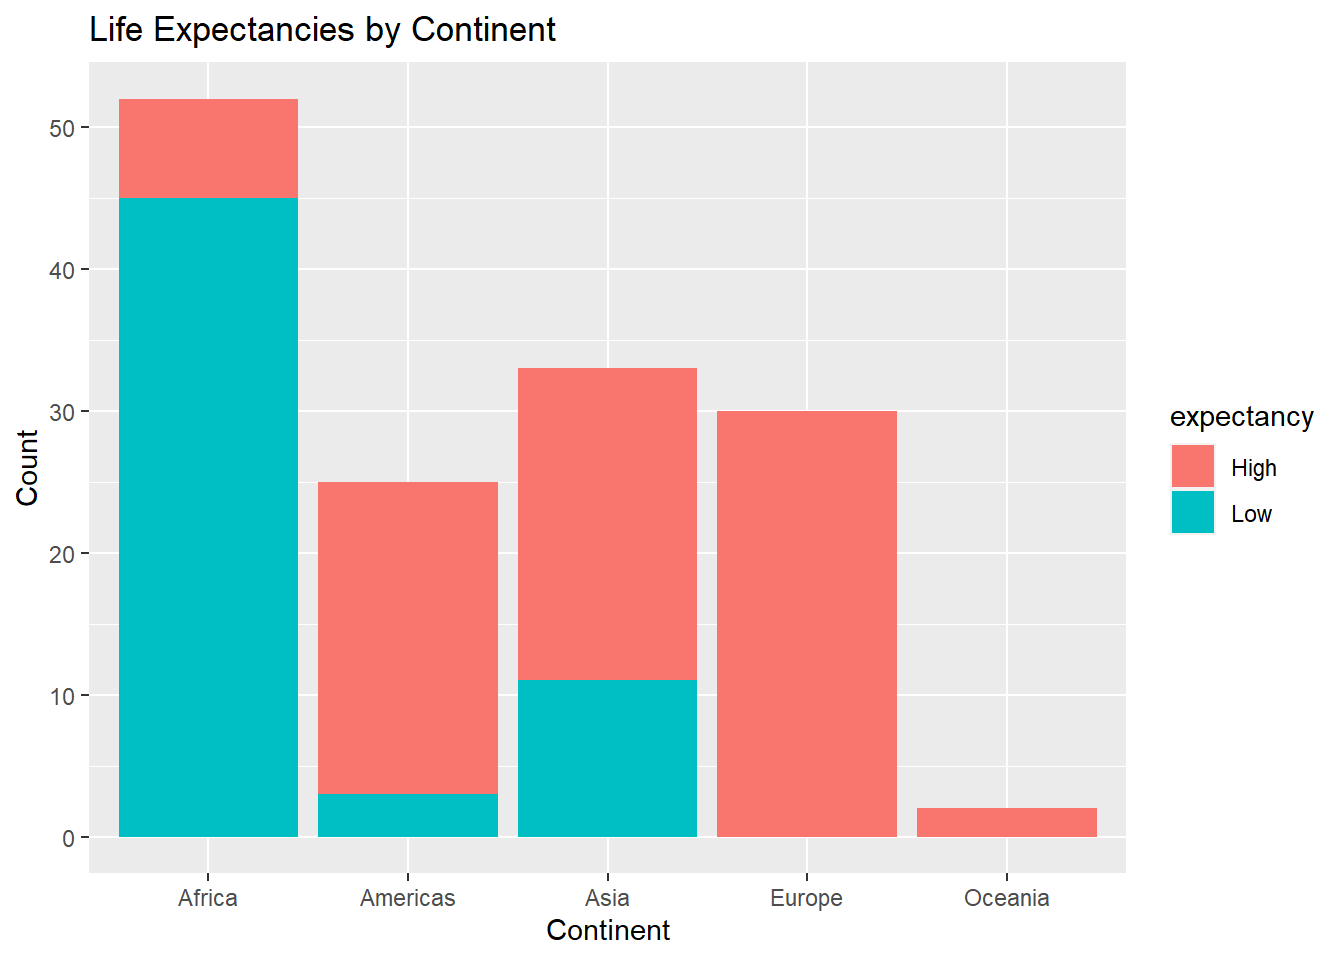
\includegraphics{bookdown-demo_files/figure-latex/unnamed-chunk-97-1.pdf}

We can see how many countries exist in each continent, and how many of these countries in each continent have high or low life expectancies. For example, there are about 25 countries in the Americas with the majority having high life expectancies.

We can change the way the bar chart is displayed by changing \texttt{position} in \texttt{geom\_bar()} to \texttt{position\ =\ "dodge"} or \texttt{position\ =\ "fill"}, the latter being more useful for proportions instead of counts:

\begin{Shaded}
\begin{Highlighting}[]
\FunctionTok{ggplot}\NormalTok{(Data, }\FunctionTok{aes}\NormalTok{(}\AttributeTok{x=}\NormalTok{continent, }\AttributeTok{fill=}\NormalTok{expectancy))}\SpecialCharTok{+}
  \FunctionTok{geom\_bar}\NormalTok{(}\AttributeTok{position =} \StringTok{"dodge"}\NormalTok{) }
\end{Highlighting}
\end{Shaded}

\begin{Shaded}
\begin{Highlighting}[]
\FunctionTok{ggplot}\NormalTok{(Data, }\FunctionTok{aes}\NormalTok{(}\AttributeTok{x=}\NormalTok{continent, }\AttributeTok{fill=}\NormalTok{expectancy))}\SpecialCharTok{+}
  \FunctionTok{geom\_bar}\NormalTok{(}\AttributeTok{position =} \StringTok{"fill"}\NormalTok{)}\SpecialCharTok{+}
  \FunctionTok{labs}\NormalTok{(}\AttributeTok{x=}\StringTok{"Continent"}\NormalTok{, }\AttributeTok{y=}\StringTok{"Proportion"}\NormalTok{, }
       \AttributeTok{title=}\StringTok{"Proportion of Life Expectancies by Continent"}\NormalTok{)}
\end{Highlighting}
\end{Shaded}

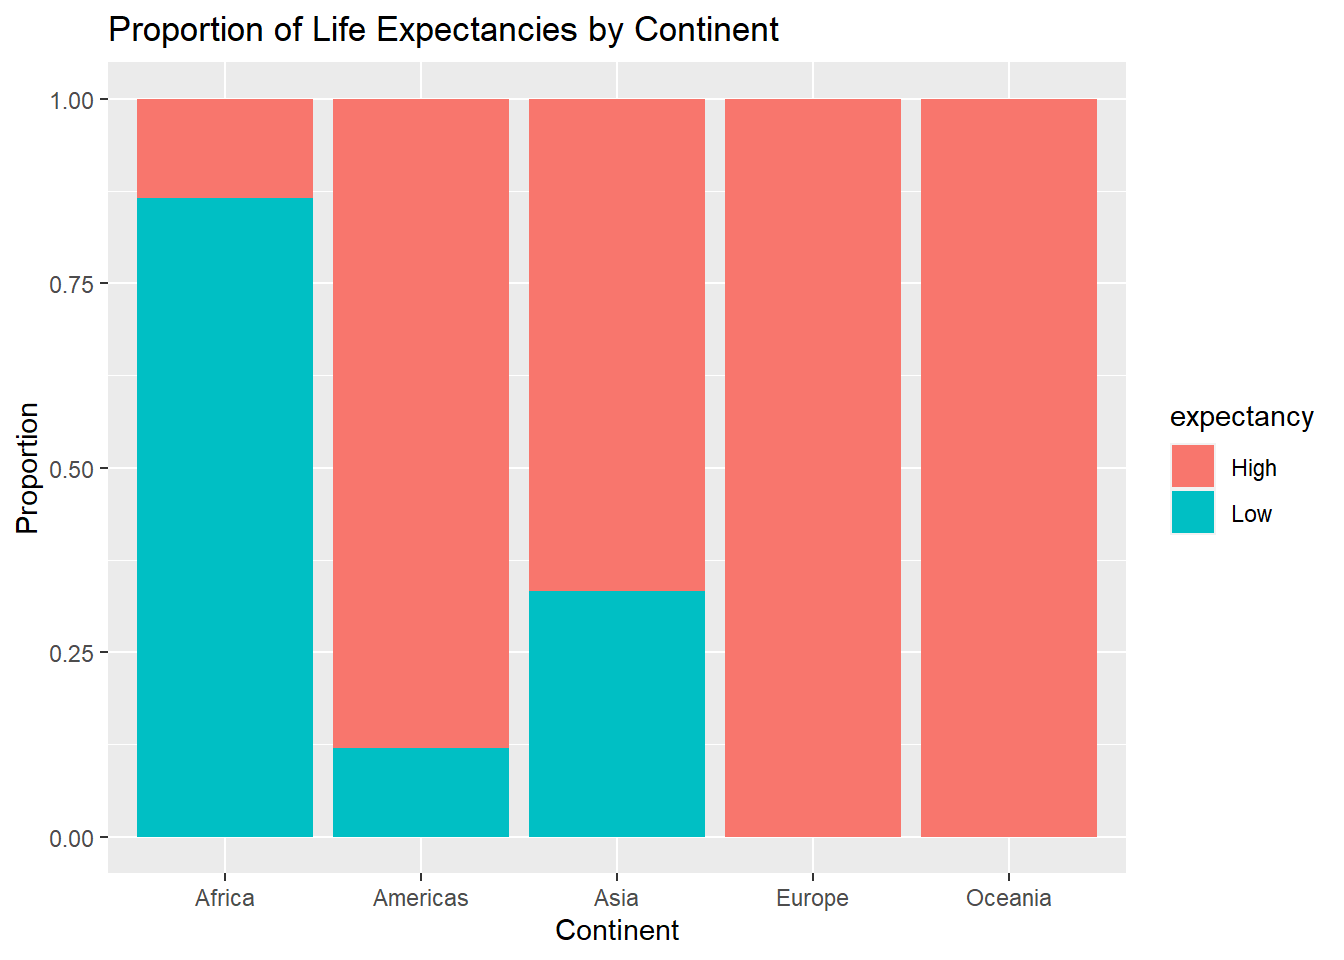
\includegraphics{bookdown-demo_files/figure-latex/unnamed-chunk-99-1.pdf}

\hypertarget{summarizing-two-quantitative-variables}{%
\subsection{Summarizing two quantitative variables}\label{summarizing-two-quantitative-variables}}

\hypertarget{scatterplots}{%
\subsubsection{Scatterplots}\label{scatterplots}}

Scatterplots are the standard visualization when two quantitative variables are involved. To create a scatterplot for life expectancy against GDP per capita:

\begin{Shaded}
\begin{Highlighting}[]
\FunctionTok{ggplot}\NormalTok{(Data, }\FunctionTok{aes}\NormalTok{(}\AttributeTok{x=}\NormalTok{gdpPercap,}\AttributeTok{y=}\NormalTok{lifeExp))}\SpecialCharTok{+}
  \FunctionTok{geom\_point}\NormalTok{()}
\end{Highlighting}
\end{Shaded}

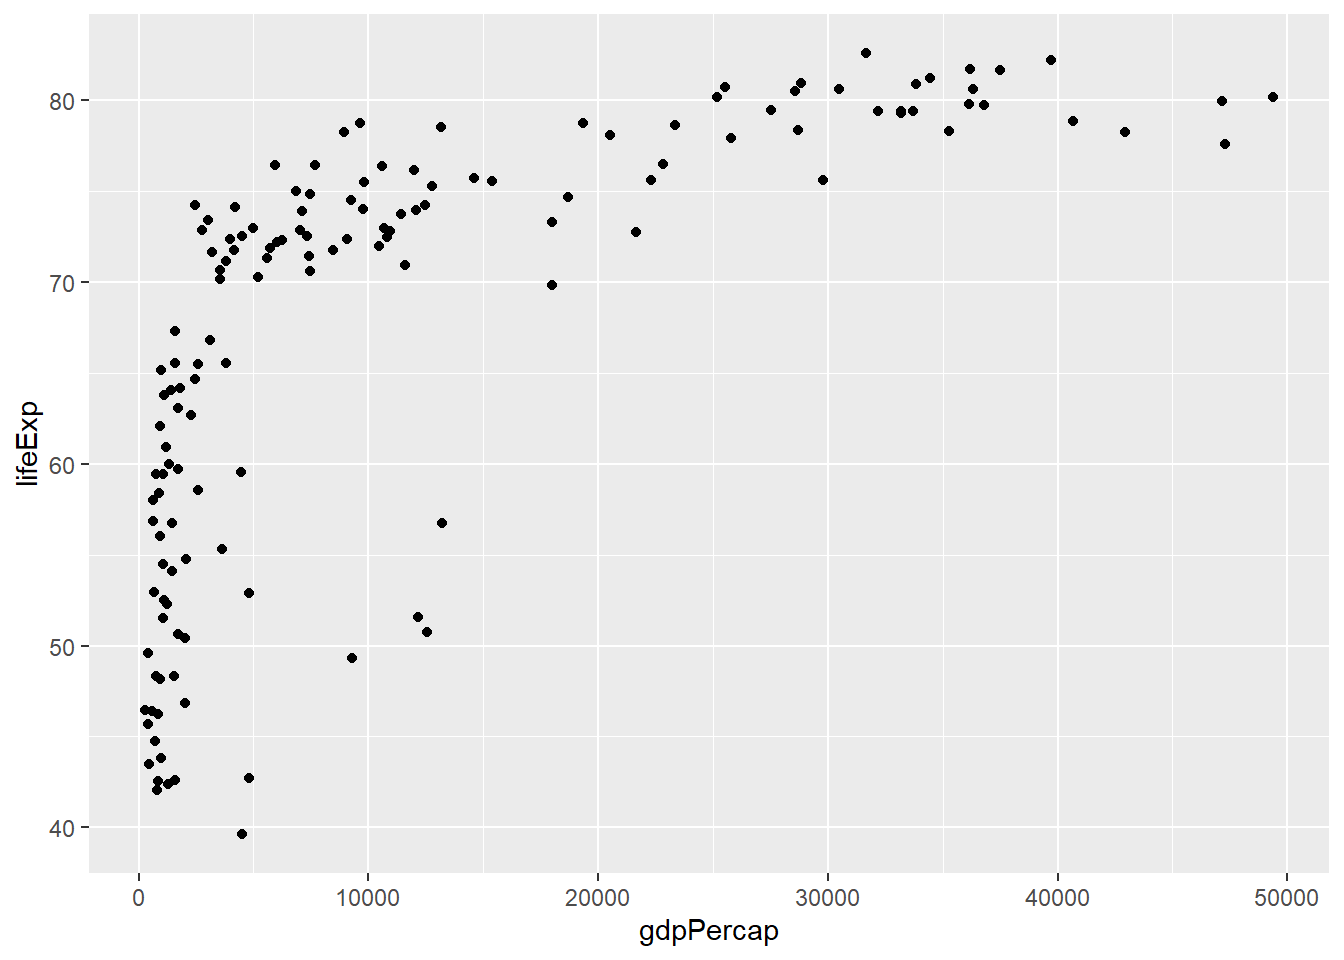
\includegraphics{bookdown-demo_files/figure-latex/unnamed-chunk-100-1.pdf}

We see a curved relationship between life expectancies and GDP per capita. Countries with higher GDP per capita tend to have longer life expectancies.

When there are many observations, plots on the scatterplot may actually overlap each other. To have a sense of how many of these exist, we can add a transparency scale called \texttt{alpha=0.2} inside \texttt{geom\_point()}:

\begin{Shaded}
\begin{Highlighting}[]
\FunctionTok{ggplot}\NormalTok{(Data, }\FunctionTok{aes}\NormalTok{(}\AttributeTok{x=}\NormalTok{gdpPercap,}\AttributeTok{y=}\NormalTok{lifeExp))}\SpecialCharTok{+}
  \FunctionTok{geom\_point}\NormalTok{(}\AttributeTok{alpha=}\FloatTok{0.2}\NormalTok{)}\SpecialCharTok{+}
  \FunctionTok{labs}\NormalTok{(}\AttributeTok{x=}\StringTok{"GDP"}\NormalTok{, }\AttributeTok{y=}\StringTok{"Life Exp"}\NormalTok{, }
       \AttributeTok{title=}\StringTok{"Scatterplot of Life Exp against GDP"}\NormalTok{)}
\end{Highlighting}
\end{Shaded}

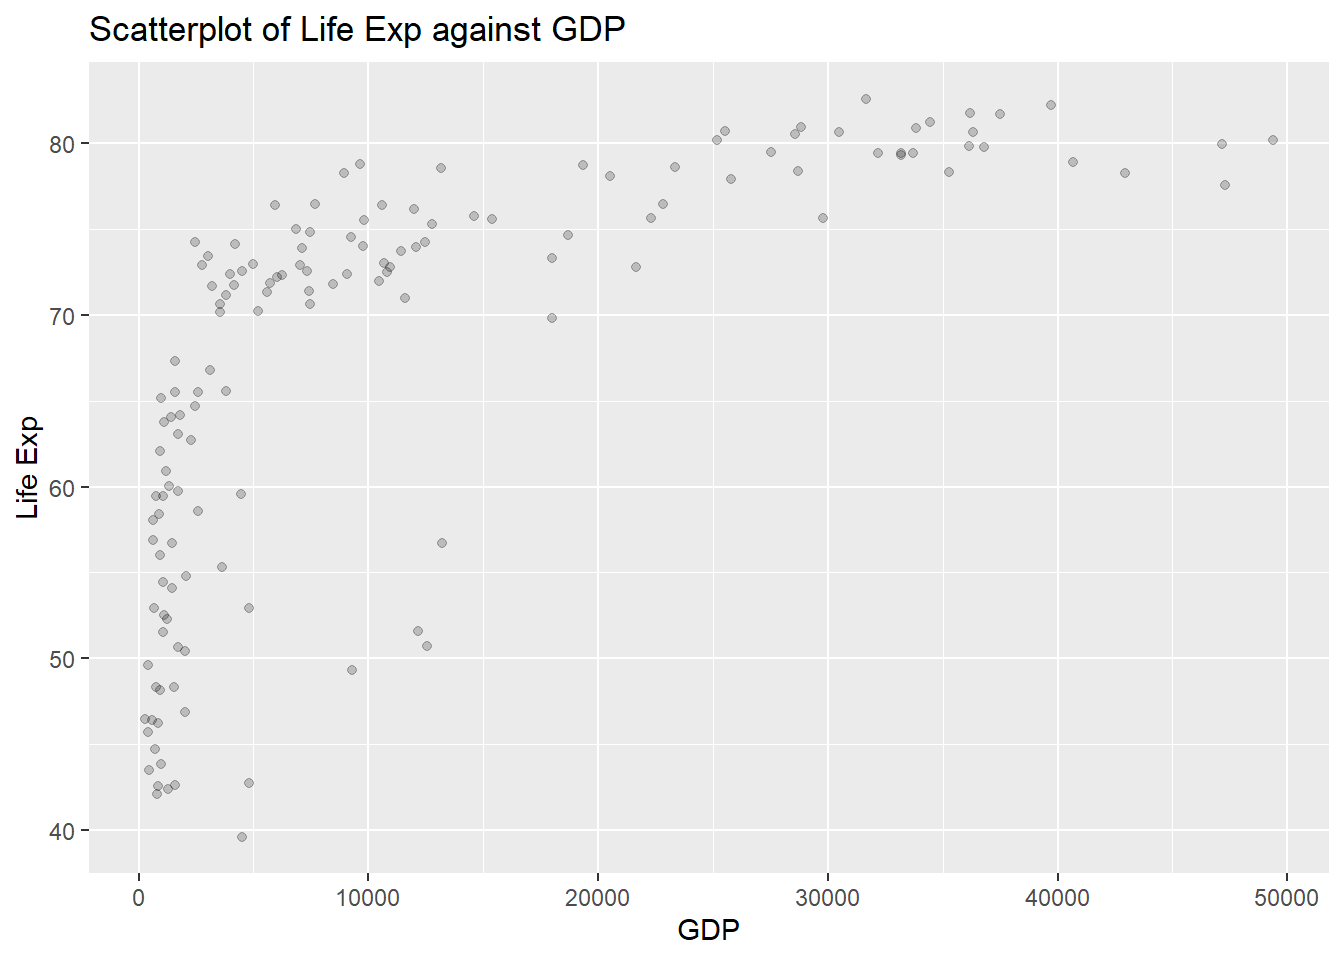
\includegraphics{bookdown-demo_files/figure-latex/unnamed-chunk-101-1.pdf}

The default value for \texttt{alpha} is 1, which means the points are not at all transparent. The closer this value is to 0, the more transparent the points are. A darker point indicates more observations with those specific values on both variables.

\hypertarget{multivariate-visualizations}{%
\section{Multivariate Visualizations}\label{multivariate-visualizations}}

We will now look at visualizations we can create to explore the relationship between multiple (more than two) variables. The term multivariate means that we are looking at more than two variables.

\hypertarget{bar-charts-2}{%
\subsection{Bar charts}\label{bar-charts-2}}

Previously, we created a bar chart to look at how \texttt{expectancy} varies across the continents. Suppose we want to see how these bar graphs vary across the years, so we use the \texttt{year} variable as a third variable via a layer \texttt{facet\_wrap}:

\begin{Shaded}
\begin{Highlighting}[]
\DocumentationTok{\#\#another data frame across all years plus a binary variable }
\DocumentationTok{\#\#for expectancy}
\NormalTok{Data.all}\OtherTok{\textless{}{-}}\NormalTok{gapminder}\SpecialCharTok{\%\textgreater{}\%}
  \FunctionTok{mutate}\NormalTok{(}\AttributeTok{expectancy=}\FunctionTok{ifelse}\NormalTok{(lifeExp}\SpecialCharTok{\textless{}}\DecValTok{70}\NormalTok{,}\StringTok{"Low"}\NormalTok{,}\StringTok{"High"}\NormalTok{))}

\FunctionTok{ggplot}\NormalTok{(Data.all,}\FunctionTok{aes}\NormalTok{(}\AttributeTok{x=}\NormalTok{continent, }\AttributeTok{fill=}\NormalTok{expectancy))}\SpecialCharTok{+}
  \FunctionTok{geom\_bar}\NormalTok{(}\AttributeTok{position =} \StringTok{"fill"}\NormalTok{)}\SpecialCharTok{+}
  \FunctionTok{facet\_wrap}\NormalTok{(}\SpecialCharTok{\textasciitilde{}}\NormalTok{year)}
\end{Highlighting}
\end{Shaded}

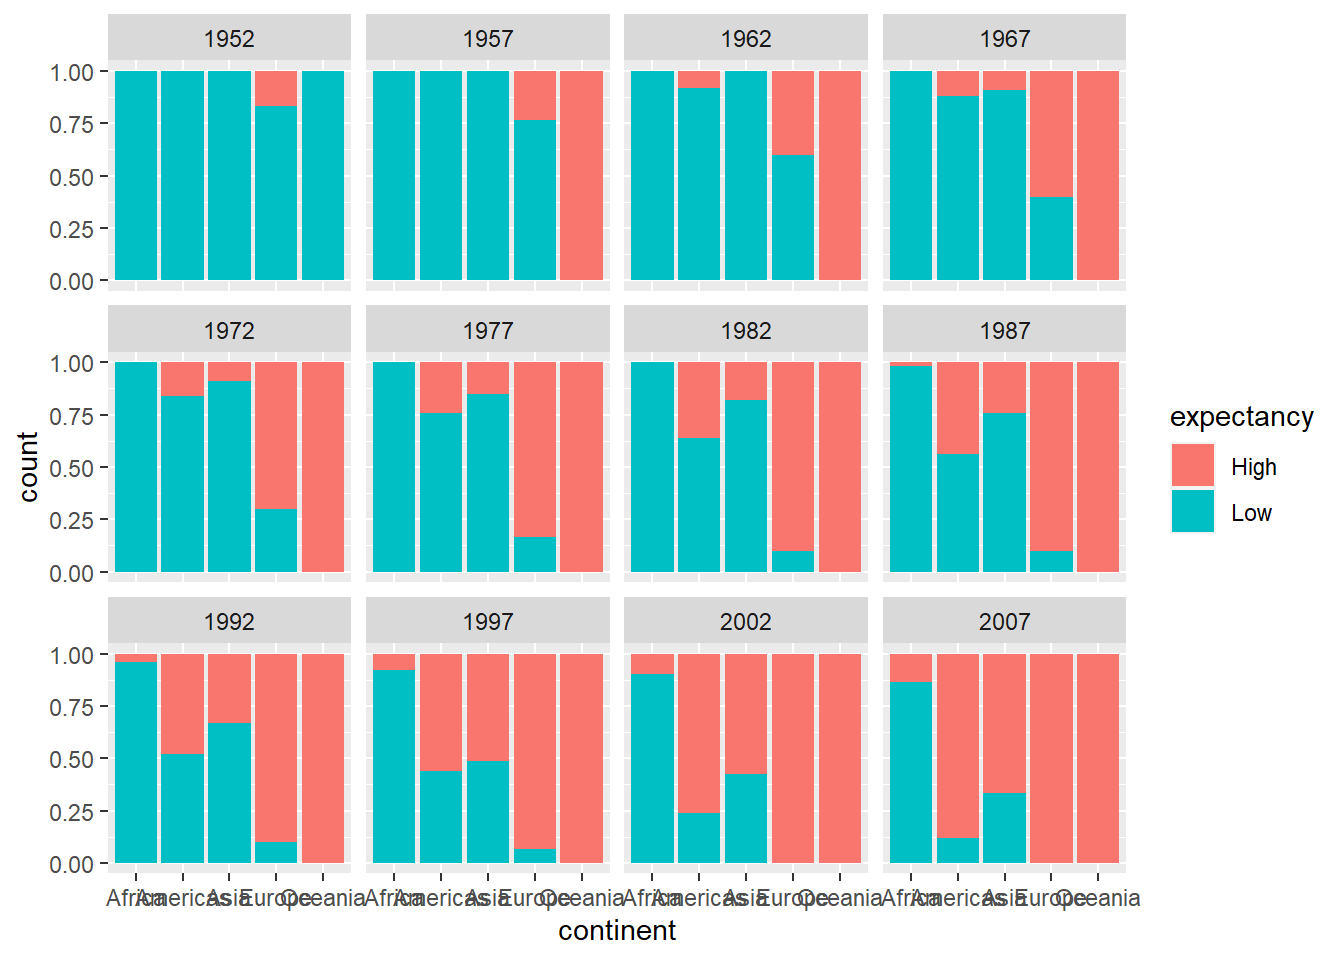
\includegraphics{bookdown-demo_files/figure-latex/unnamed-chunk-102-1.pdf}

Notice that three categorical variables are summarized in this bar chart. Is there something that can be done to improve this bar chart? How would you make this improvement?

\hypertarget{scatterplots-1}{%
\subsection{Scatterplots}\label{scatterplots-1}}

Previously, we created a scatterplot of life expectancy against GDP per capita. We can include another quantitative variable in the scatterplot, by using the size of the plots. We can use the size of the plots to denote the population of the countries. This is supplied via \texttt{size} in \texttt{aes()}:

\begin{Shaded}
\begin{Highlighting}[]
\FunctionTok{ggplot}\NormalTok{(Data, }\FunctionTok{aes}\NormalTok{(}\AttributeTok{x=}\NormalTok{gdpPercap, }\AttributeTok{y=}\NormalTok{lifeExp, }\AttributeTok{size=}\NormalTok{pop))}\SpecialCharTok{+}
  \FunctionTok{geom\_point}\NormalTok{()}
\end{Highlighting}
\end{Shaded}

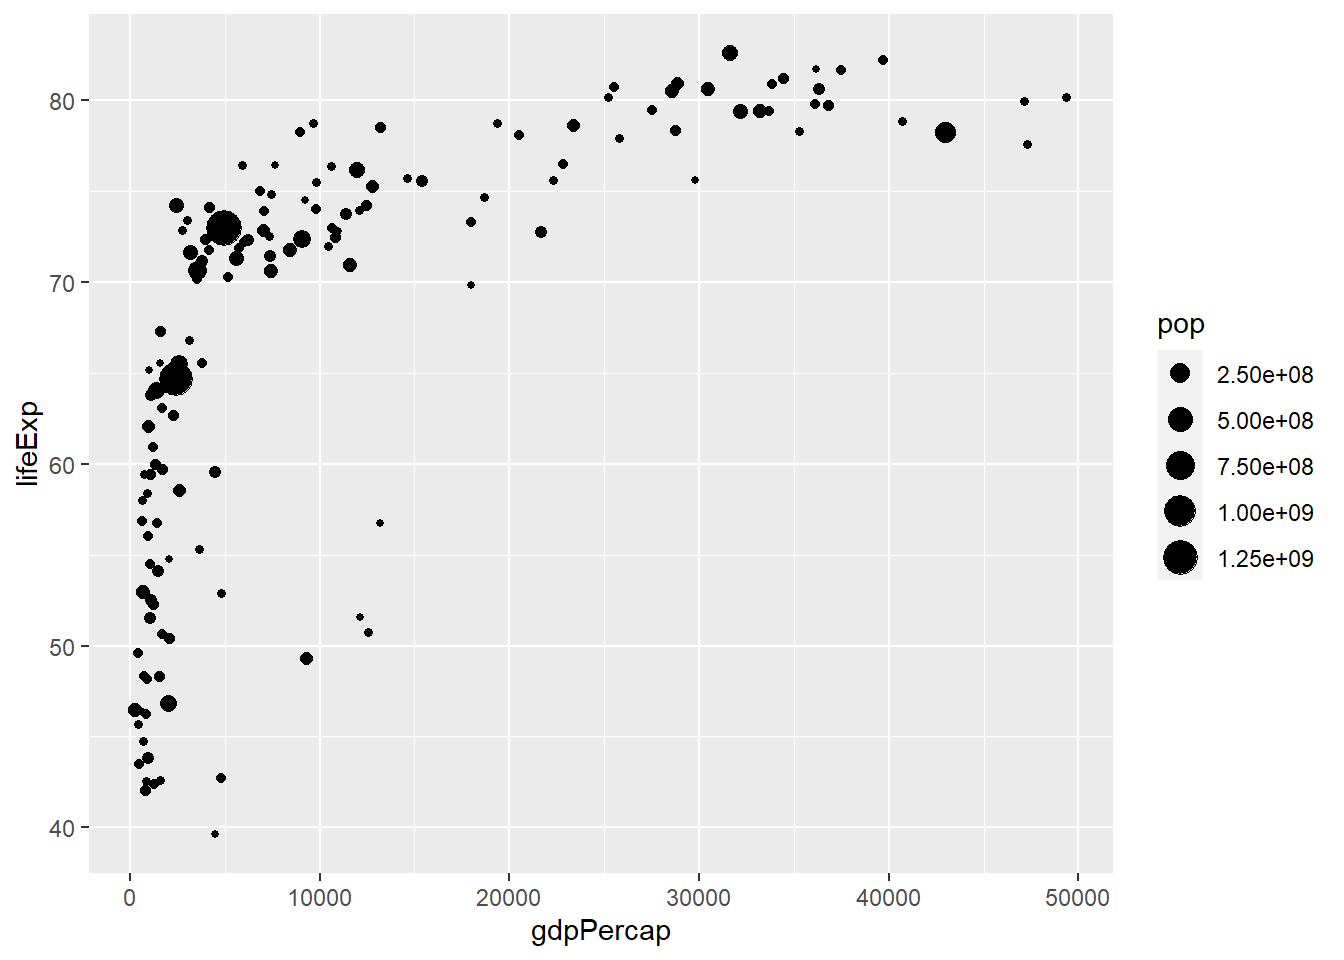
\includegraphics{bookdown-demo_files/figure-latex/unnamed-chunk-103-1.pdf}

We can adjust the size of the plots by adding a layer \texttt{scale\_size()}:

\begin{Shaded}
\begin{Highlighting}[]
\FunctionTok{ggplot}\NormalTok{(Data, }\FunctionTok{aes}\NormalTok{(}\AttributeTok{x=}\NormalTok{gdpPercap, }\AttributeTok{y=}\NormalTok{lifeExp, }\AttributeTok{size=}\NormalTok{pop))}\SpecialCharTok{+}
  \FunctionTok{geom\_point}\NormalTok{()}\SpecialCharTok{+}
  \FunctionTok{scale\_size}\NormalTok{(}\AttributeTok{range =} \FunctionTok{c}\NormalTok{(}\FloatTok{0.1}\NormalTok{,}\DecValTok{12}\NormalTok{))}
\end{Highlighting}
\end{Shaded}

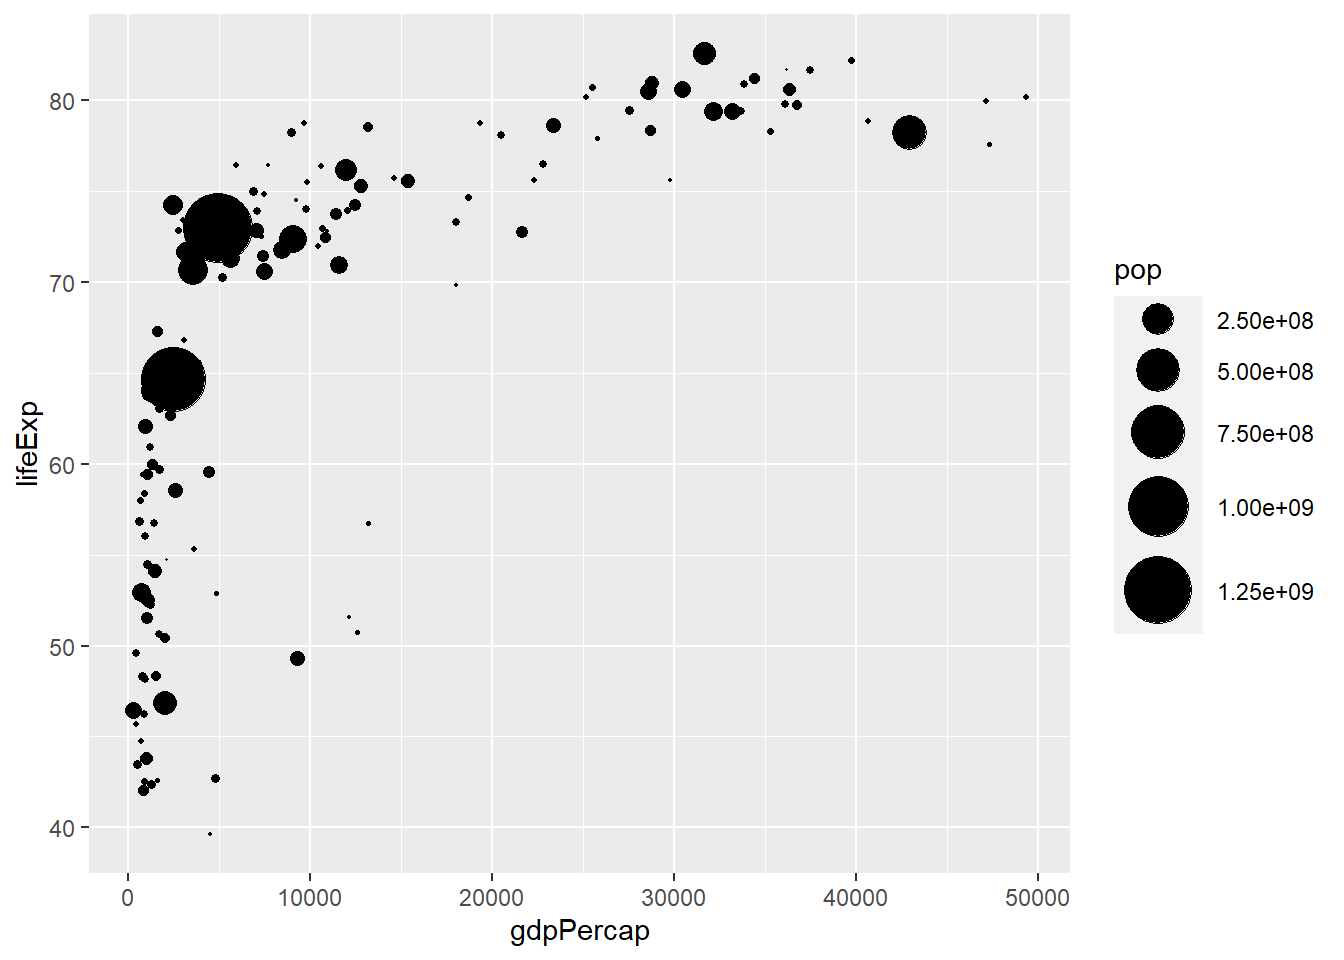
\includegraphics{bookdown-demo_files/figure-latex/unnamed-chunk-104-1.pdf}

This scatterplot summarizes three quantitative variables.

We can use different-colored plots to denote which continent each point belongs to:

\begin{Shaded}
\begin{Highlighting}[]
\FunctionTok{ggplot}\NormalTok{(Data, }\FunctionTok{aes}\NormalTok{(}\AttributeTok{x=}\NormalTok{gdpPercap, }\AttributeTok{y=}\NormalTok{lifeExp, }\AttributeTok{size=}\NormalTok{pop, }\AttributeTok{color=}\NormalTok{continent))}\SpecialCharTok{+}
  \FunctionTok{geom\_point}\NormalTok{()}\SpecialCharTok{+}
  \FunctionTok{scale\_size}\NormalTok{(}\AttributeTok{range =} \FunctionTok{c}\NormalTok{(}\FloatTok{0.1}\NormalTok{,}\DecValTok{12}\NormalTok{))}
\end{Highlighting}
\end{Shaded}

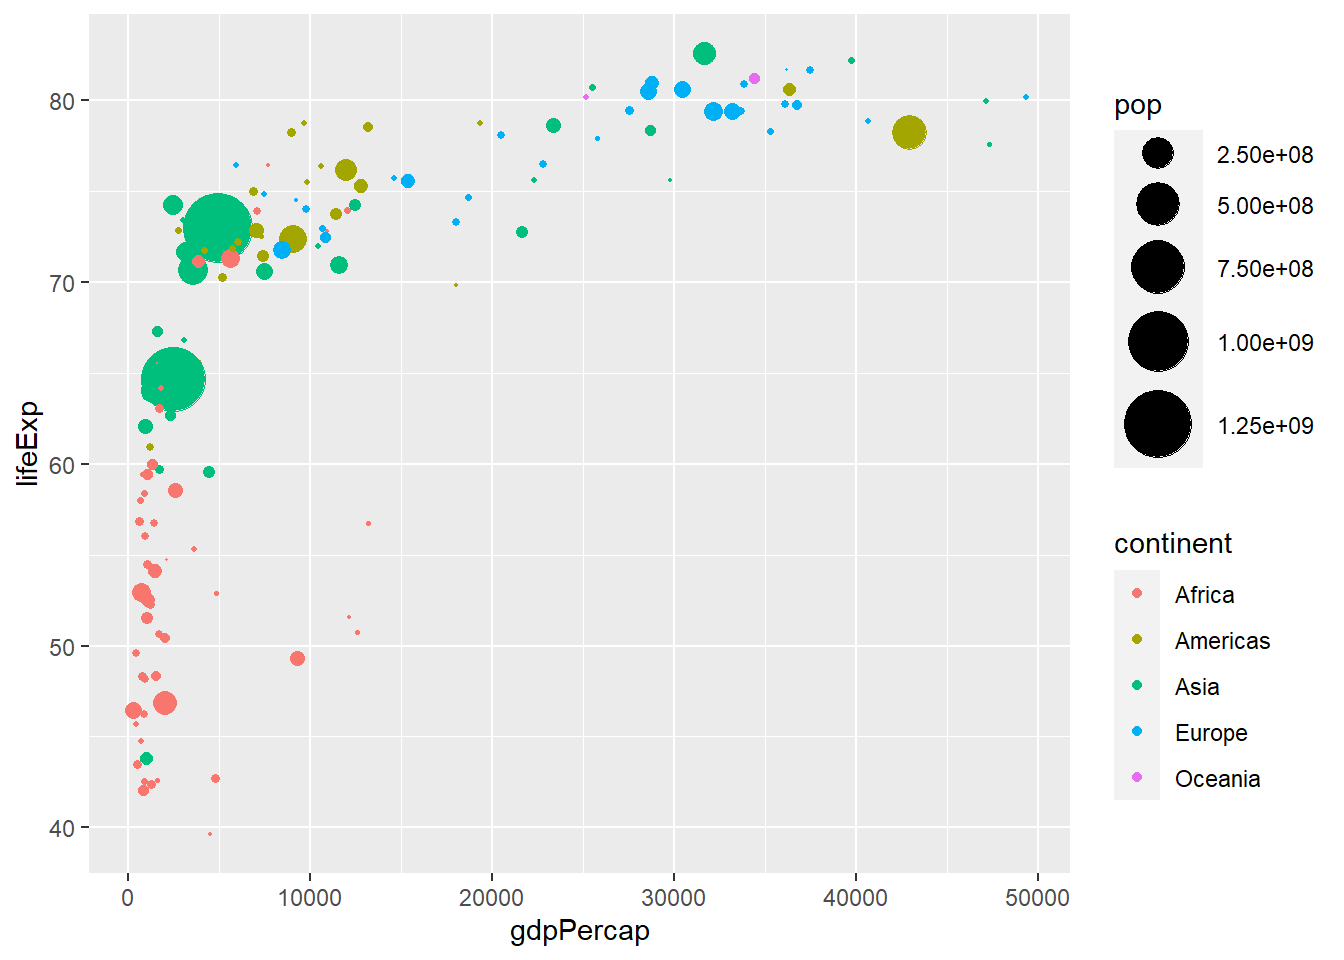
\includegraphics{bookdown-demo_files/figure-latex/unnamed-chunk-105-1.pdf}

This scatterplot summarizes three quantitative variables and one categorical variable.

We can adjust the plots by changing its shape and making it more translucent via \texttt{shape} and \texttt{alpha} in \texttt{aes()}:

\begin{Shaded}
\begin{Highlighting}[]
\FunctionTok{ggplot}\NormalTok{(Data, }\FunctionTok{aes}\NormalTok{(}\AttributeTok{x=}\NormalTok{gdpPercap, }\AttributeTok{y=}\NormalTok{lifeExp, }\AttributeTok{size=}\NormalTok{pop, }\AttributeTok{fill=}\NormalTok{continent))}\SpecialCharTok{+}
  \FunctionTok{geom\_point}\NormalTok{(}\AttributeTok{shape=}\DecValTok{21}\NormalTok{, }\AttributeTok{alpha=}\FloatTok{0.5}\NormalTok{)}\SpecialCharTok{+}
  \FunctionTok{scale\_size}\NormalTok{(}\AttributeTok{range =} \FunctionTok{c}\NormalTok{(}\FloatTok{0.1}\NormalTok{,}\DecValTok{12}\NormalTok{))}\SpecialCharTok{+}
  \FunctionTok{labs}\NormalTok{(}\AttributeTok{x=}\StringTok{"GDP"}\NormalTok{, }\AttributeTok{y=}\StringTok{"Life Exp"}\NormalTok{, }\AttributeTok{title=}\StringTok{"Scatterplot of Life Exp against GDP"}\NormalTok{)}
\end{Highlighting}
\end{Shaded}

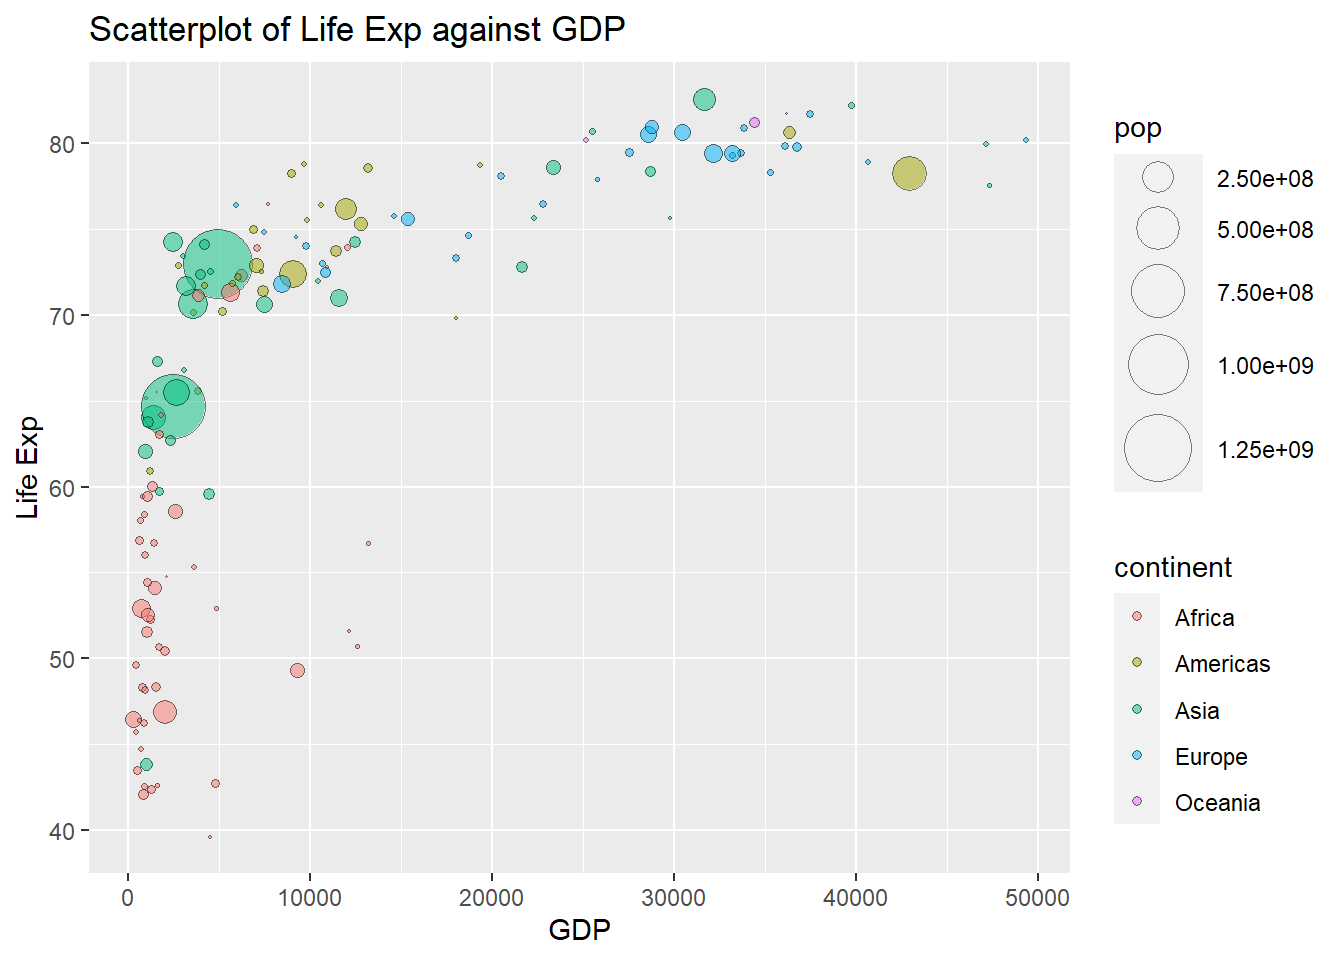
\includegraphics{bookdown-demo_files/figure-latex/unnamed-chunk-106-1.pdf}

\hypertarget{slr}{%
\chapter{Basics with Simple Linear Regression (SLR)}\label{slr}}

\hypertarget{introduction-2}{%
\section{Introduction}\label{introduction-2}}

We will start this module by introducing the simple linear regression model. Simple linear regression uses the term ``simple,'' because it concerns the study of only one predictor variable with one quantitative response variable. In contrast, multiple linear regression, which we will study in future modules, uses the term ``multiple,'' because it concerns the study of two or more predictor variables with one quantitative response variable. We start with simple linear regression as it is much easier to visualize concepts in regression models when there is only one predictor variable.

For the time being, we will only consider predictor variables that are quantitative. We will consider predictor variables that are categorical in future modules.

The most common way of visualizing the relationship between one quantitative predictor variable and one quantitative response variable is with a scatter plot. In the simulated example below, we have data from 6000 UVa undergraduate students on the amount of time they spend studying in a week (in minutes), and how many courses they are taking in the semester (3 or 4 credit courses).

\begin{Shaded}
\begin{Highlighting}[]
\DocumentationTok{\#\#create dataframe}
\NormalTok{df}\OtherTok{\textless{}{-}}\FunctionTok{data.frame}\NormalTok{(study,courses)}

\DocumentationTok{\#\#fit regression}
\NormalTok{result}\OtherTok{\textless{}{-}}\FunctionTok{lm}\NormalTok{(study}\SpecialCharTok{\textasciitilde{}}\NormalTok{courses, }\AttributeTok{data=}\NormalTok{df)}
\end{Highlighting}
\end{Shaded}

\begin{Shaded}
\begin{Highlighting}[]
\DocumentationTok{\#\#create scatterplot with regression line overlaid}
\FunctionTok{plot}\NormalTok{(df}\SpecialCharTok{$}\NormalTok{courses, df}\SpecialCharTok{$}\NormalTok{study, }\AttributeTok{xlab=}\StringTok{"\# of Courses"}\NormalTok{, }\AttributeTok{ylab=}\StringTok{"Study Time (Mins)"}\NormalTok{)}
\FunctionTok{abline}\NormalTok{(result)}
\end{Highlighting}
\end{Shaded}

\begin{figure}
\centering
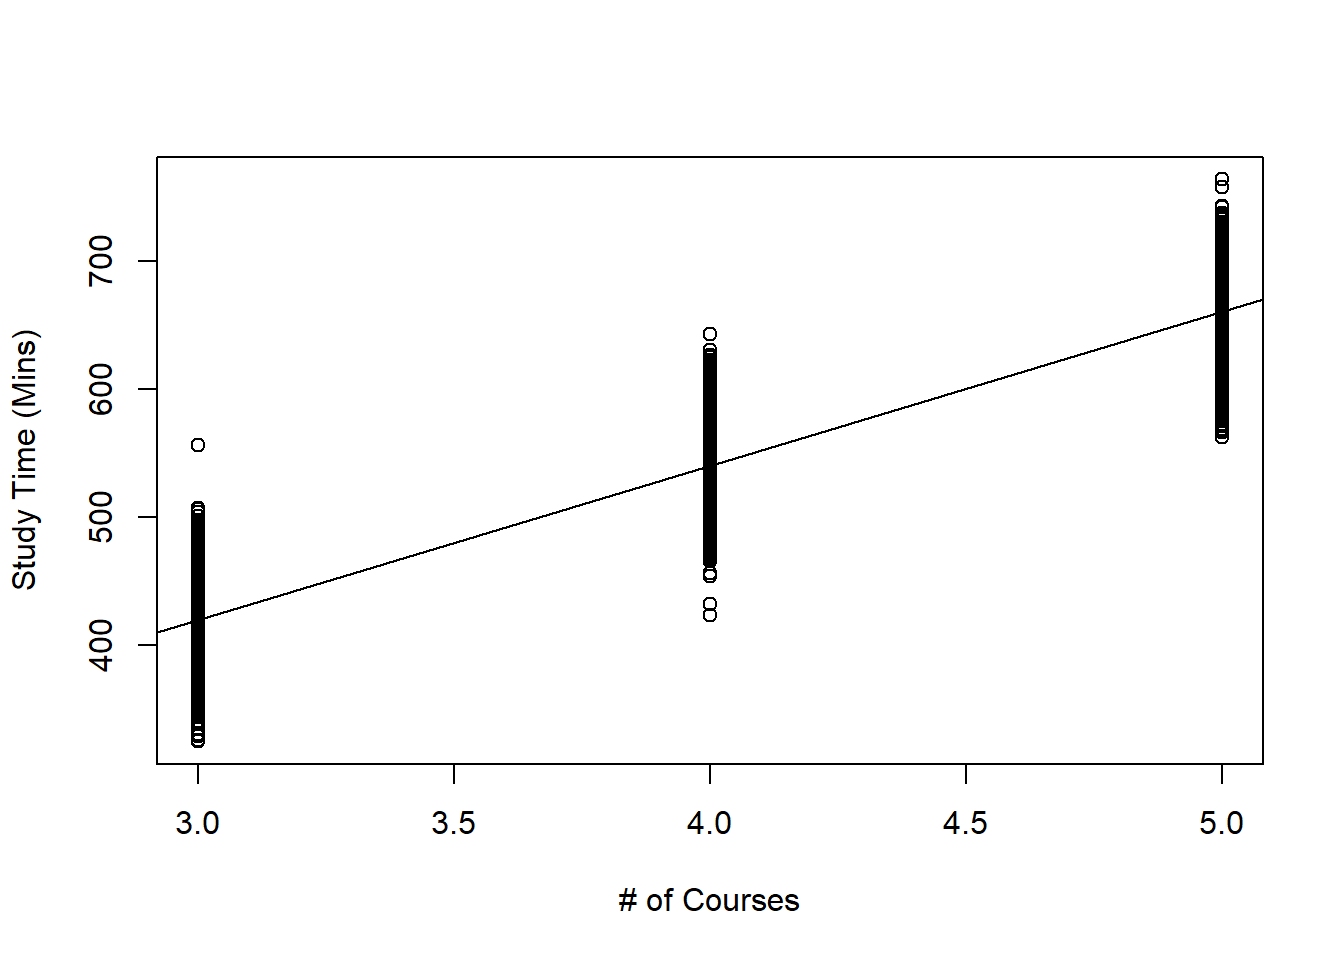
\includegraphics{bookdown-demo_files/figure-latex/scatter-courses-1.pdf}
\caption{\label{fig:scatter-courses}Scatterplot of Study Time against Number of Courses Taken}
\end{figure}

Questions that we may have include:

\begin{itemize}
\tightlist
\item
  Are study time and the number of courses taken related to one another?
\item
  How strong is this relationship?
\item
  Could we use the data to make a prediction for the study time of a student who is not in this scatterplot?
\item
  How confident are we of the prediction?
\end{itemize}

These questions can be answered using simple linear regression.

Note that we will only be learning about models with just one response variable. We will not cover multivariate regression, which is used when there is more than one response variable. There may be some confusion between ``multiple'' linear regression and ``multivariate'' regression due to the closeness in terminology.

\hypertarget{basic-ideas-with-statistics}{%
\subsection{Basic Ideas with Statistics}\label{basic-ideas-with-statistics}}

\hypertarget{population-vs-sample}{%
\subsubsection{Population vs Sample}\label{population-vs-sample}}

Statistical methods are usually used to make inferences about the \textbf{population} based on information from a \textbf{sample}.

\begin{itemize}
\tightlist
\item
  A sample is the collection of units that is actually measured or surveyed in a study.
\item
  The population includes all units of interest.
\end{itemize}

In the study time example above, the population is all UVa undergraduate students, while the sample is the 6000 students that we have data on and are displayed on the scatterplot.

\hypertarget{parameters-vs-statistics}{%
\subsubsection{Parameters vs Statistics}\label{parameters-vs-statistics}}

\begin{itemize}
\tightlist
\item
  \textbf{Parameters} are numerical quantities that describe a population.
\item
  \textbf{Statistics} are numerical quantities that describe a sample.
\end{itemize}

In the study time example, an example of a parameter will be the average study time among all UVa undergraduate students (called the population mean), and an example of a statistic will be the average study time among the 6000 UVa students we have data on (called the sample mean).

Notice that in real life, we will rarely know the actual numerical value of a parameter. So we use the numerical value of the statistic to \textbf{estimate} the unknown numerical value of the corresponding parameter.

We also have different notation for parameters and statistics. For example,

\begin{itemize}
\tightlist
\item
  the population mean is denoted as \(\mu\).
\item
  the sample mean is denoted as \(\bar{x}\).
\end{itemize}

We say that \(\bar{x}\) is an \textbf{estimator} of \(\mu\).

It is important to pay attention to whether we are describing a statistic (a known value that can be calculated) or a parameter (an unknown value).

\hypertarget{motivation}{%
\subsection{Motivation}\label{motivation}}

Linear regression models generally have two primary uses:

\begin{enumerate}
\def\labelenumi{\arabic{enumi}.}
\tightlist
\item
  \textbf{Prediction}: Predict a future value of a response variable, using information from predictor variables.
\item
  \textbf{Association}: Quantify the relationship between variables. How does a change in the predictor variable change the value of the response variable?
\end{enumerate}

We always distinguish between a \textbf{response variable, denoted by \(y\)}, and a \textbf{predictor variable, denoted by \(x\)}. In most statistical models, we say that the response variable can be approximated by some \textbf{mathematical function, denoted by \(f\)}, of the predictor variable, i.e.

\[
y \approx f(x).
\]
Oftentimes, we write this relationship as

\[
y = f(x) + \epsilon,
\]

where \textbf{\(\epsilon\) denotes a random error term}, with a mean of 0. The error term cannot be predicted based on the data we have.

There are various statistical methods to estimate \(f\). Once we estimate \(f\), we can use our method for prediction and / or association.

Using the study time example above:

\begin{itemize}
\tightlist
\item
  a prediction example: a student intends to take 4 courses in the semester. What is this student's predicted study time, on average?
\item
  an association example: we want to see how taking more courses increases study time.
\end{itemize}

\hypertarget{practice-questions}{%
\subsubsection{Practice questions}\label{practice-questions}}

In the examples below, are we using a regression model for prediction or for association?

\begin{enumerate}
\def\labelenumi{\arabic{enumi}.}
\item
  It is early in the morning and I am heading out for the rest of the day. I want to know the weather forecast for the rest of the day so I know what to wear.
\item
  An executive for a sports league wants to assess how increasing the length of commercial breaks may impact the enjoyment of sports fans who watch games on TV.
\item
  The Education Secretary would like to evaluate how certain factors such as use of technology in classrooms and investment in teacher training and teacher pay are associated with reading skills of students.
\item
  When buying a home, the prospective buyer would like to know if the home is under- or over- priced, given its characteristics.
\end{enumerate}

\hypertarget{simple-linear-regression-slr}{%
\section{Simple Linear Regression (SLR)}\label{simple-linear-regression-slr}}

In simple linear regression (SLR), the function \(f\) that relates the predictor variable with the response variable is typically \(\beta_0 + \beta_1 x\). Mathematically, we express this as

\[
y \approx \beta_0 + \beta_1 x,
\]

or in other words, that the response variable has an approximately linear relationship with the predictor variable.

In SLR, this relationship is more explicitly formulated as the \textbf{simple linear regression equation}:

\begin{equation} 
E(y|x)=\beta_0+\beta_{1}x.
\label{eq:SLR}
\end{equation}

\begin{itemize}
\item
  \(\beta_0\) and \(\beta_1\) are parameters in the SLR equation, and we want to estimate them.
\item
  These parameters are sometimes called \textbf{regression coefficients}.
\item
  \(\beta_1\) is also called the \textbf{slope. It denotes the change in \(y\), on average, when \(x\) increases by one unit.}
\item
  \(\beta_0\) is also called the \textbf{intercept. It denotes the average of \(y\) when \(x=0\).}
\item
  The notation on the left hand side of \eqref{eq:SLR} denotes the \textbf{expected value} of the response variable, for a fixed value of the predictor variable. What \eqref{eq:SLR} implies is that, for each value of the predictor variable \(x\), the expected value of the response variable \(y\) is \(\beta_0+\beta_{1}x\). The expected value is also the population mean. Applying \eqref{eq:SLR} to our study time example, it implies that:

  \begin{itemize}
  \tightlist
  \item
    for students who take 3 courses, their expected study time is equal to \(\beta_0 + 3\beta_1\),
  \item
    for students who take 4 courses, their expected study time is equal to \(\beta_0 + 4\beta_1\),
  \item
    for students who take 5 courses, their expected study time is equal to \(\beta_0 + 5\beta_1\).
  \end{itemize}
\end{itemize}

So \(f(x) = \beta_0 + \beta_1x\) gives us the value of the expected value of the response variable for a specific value of the predictor variable. But, for each value of the predictor variable, the value of the response variable is not a constant. We say that for each value of \(x\), the response variable \(y\) has some variance. The variance of the response variable for each value of \(x\) is the same as the variance of the error term, \(\epsilon\). Thus we have the \textbf{simple linear regression model}

\begin{equation} 
y=\beta_0+\beta_{1} x + \epsilon. 
\label{eq:SLRmod}
\end{equation}

We need to make some assumptions for the error term \(\epsilon\). Generally, the assumptions are:

\begin{enumerate}
\def\labelenumi{\arabic{enumi}.}
\tightlist
\item
  The errors have mean 0.
\item
  The \textbf{errors have variance denoted by \(\sigma^2\)}. Notice this variance is constant.
\item
  The errors are independent.
\item
  The errors are normally distributed.
\end{enumerate}

From \eqref{eq:SLRmod}, notice we have another parameter, \(\sigma^2\).

We will go into more detail about what these assumptions mean, and how to assess whether they are met, in module \ref{diag}.

What these assumptions mean is that for each value of the predictor variable \(x\), the response variable:

\begin{enumerate}
\def\labelenumi{\arabic{enumi}.}
\tightlist
\item
  follows a normal distribution,
\item
  with mean equal to \(\beta_0+\beta_{1} x\),
\item
  and variance equal to \(\sigma^2\).
\end{enumerate}

Using our study time example, it means that:

\begin{itemize}
\tightlist
\item
  for students who take 3 courses, the distribution of their study times is \(N(\beta_0 + 3\beta_1, \sigma^2)\).
\item
  for students who take 4 courses, the distribution of their study times is \(N(\beta_0 + 4\beta_1, \sigma^2)\).
\item
  for students who take 5 courses, the distribution of their study times is \(N(\beta_0 + 5\beta_1, \sigma^2)\).
\end{itemize}

So if we were to subset our dataframe into three subsets, one with students who take 3 courses, another subset for students who take 4 courses, and another subset for students who take 5 courses, and then create a density plot of study times for each subset, each density plot should follow a normal distribution, with different means, and the same spread.

Let us take a look at these density plots next.

\begin{Shaded}
\begin{Highlighting}[]
\FunctionTok{library}\NormalTok{(tidyverse)}
\end{Highlighting}
\end{Shaded}

\begin{Shaded}
\begin{Highlighting}[]
\DocumentationTok{\#\#subset dataframe}
\NormalTok{x}\FloatTok{.3}\OtherTok{\textless{}{-}}\NormalTok{df[}\FunctionTok{which}\NormalTok{(df}\SpecialCharTok{$}\NormalTok{courses}\SpecialCharTok{==}\DecValTok{3}\NormalTok{),]}
\DocumentationTok{\#\#density plot of study time for students taking 3 courses}
\FunctionTok{ggplot}\NormalTok{(x}\FloatTok{.3}\NormalTok{,}\FunctionTok{aes}\NormalTok{(}\AttributeTok{x=}\NormalTok{study))}\SpecialCharTok{+}
  \FunctionTok{geom\_density}\NormalTok{()}\SpecialCharTok{+}
  \FunctionTok{labs}\NormalTok{(}\AttributeTok{x=}\StringTok{"Study Time (Mins)"}\NormalTok{, }\AttributeTok{title=}\StringTok{"Dist of Study Times with 3 Courses"}\NormalTok{)}
\end{Highlighting}
\end{Shaded}

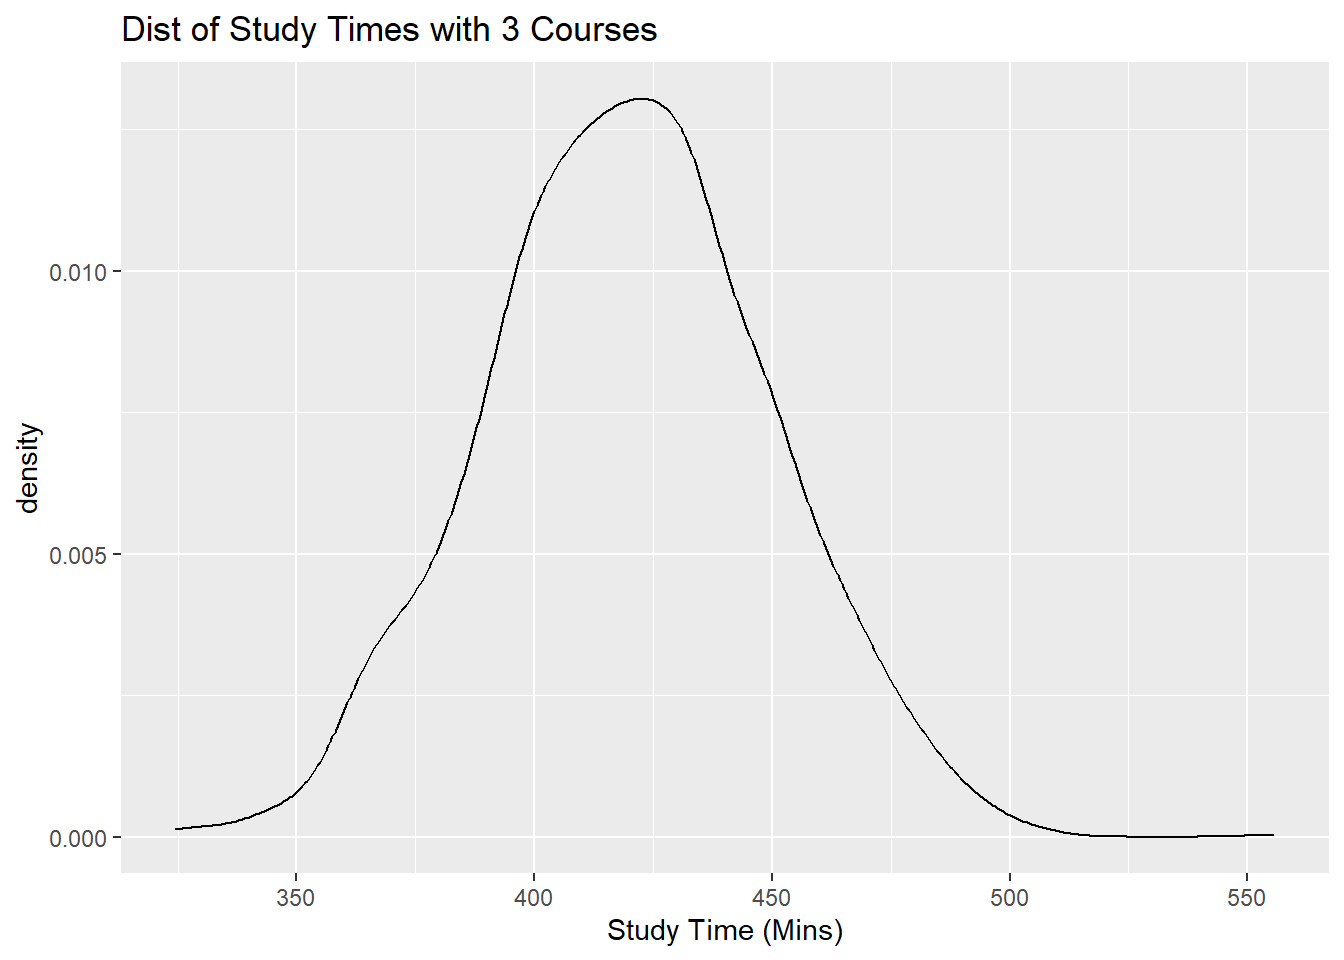
\includegraphics{bookdown-demo_files/figure-latex/unnamed-chunk-111-1.pdf}

\begin{Shaded}
\begin{Highlighting}[]
\DocumentationTok{\#\#subset dataframe}
\NormalTok{x}\FloatTok{.4}\OtherTok{\textless{}{-}}\NormalTok{df[}\FunctionTok{which}\NormalTok{(df}\SpecialCharTok{$}\NormalTok{courses}\SpecialCharTok{==}\DecValTok{4}\NormalTok{),]}
\DocumentationTok{\#\#density plot of study time for students taking 4 courses}
\FunctionTok{ggplot}\NormalTok{(x}\FloatTok{.4}\NormalTok{,}\FunctionTok{aes}\NormalTok{(}\AttributeTok{x=}\NormalTok{study))}\SpecialCharTok{+}
  \FunctionTok{geom\_density}\NormalTok{()}\SpecialCharTok{+}
  \FunctionTok{labs}\NormalTok{(}\AttributeTok{x=}\StringTok{"Study Time (Mins)"}\NormalTok{, }\AttributeTok{title=}\StringTok{"Dist of Study Times with 4 Courses"}\NormalTok{)}
\end{Highlighting}
\end{Shaded}

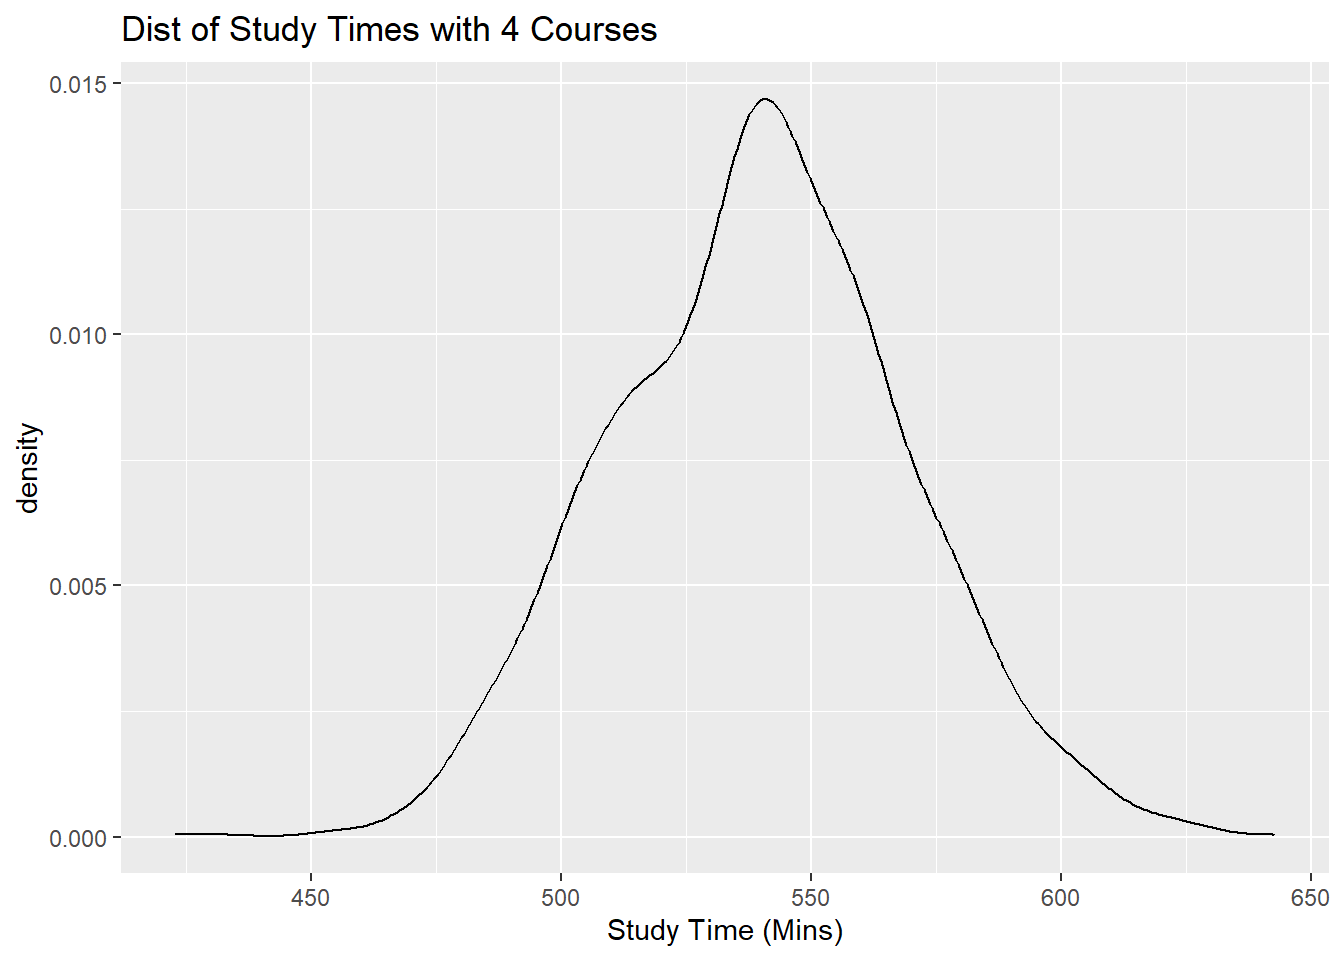
\includegraphics{bookdown-demo_files/figure-latex/unnamed-chunk-111-2.pdf}

\begin{Shaded}
\begin{Highlighting}[]
\DocumentationTok{\#\#subset dataframe}
\NormalTok{x}\FloatTok{.5}\OtherTok{\textless{}{-}}\NormalTok{df[}\FunctionTok{which}\NormalTok{(df}\SpecialCharTok{$}\NormalTok{courses}\SpecialCharTok{==}\DecValTok{5}\NormalTok{),]}
\DocumentationTok{\#\#density plot of study time for students taking 5 courses}
\FunctionTok{ggplot}\NormalTok{(x}\FloatTok{.5}\NormalTok{,}\FunctionTok{aes}\NormalTok{(}\AttributeTok{x=}\NormalTok{study))}\SpecialCharTok{+}
  \FunctionTok{geom\_density}\NormalTok{()}\SpecialCharTok{+}
  \FunctionTok{labs}\NormalTok{(}\AttributeTok{x=}\StringTok{"Study Time (Mins)"}\NormalTok{, }\AttributeTok{title=}\StringTok{"Dist of Study Times with 5 Courses"}\NormalTok{)}
\end{Highlighting}
\end{Shaded}

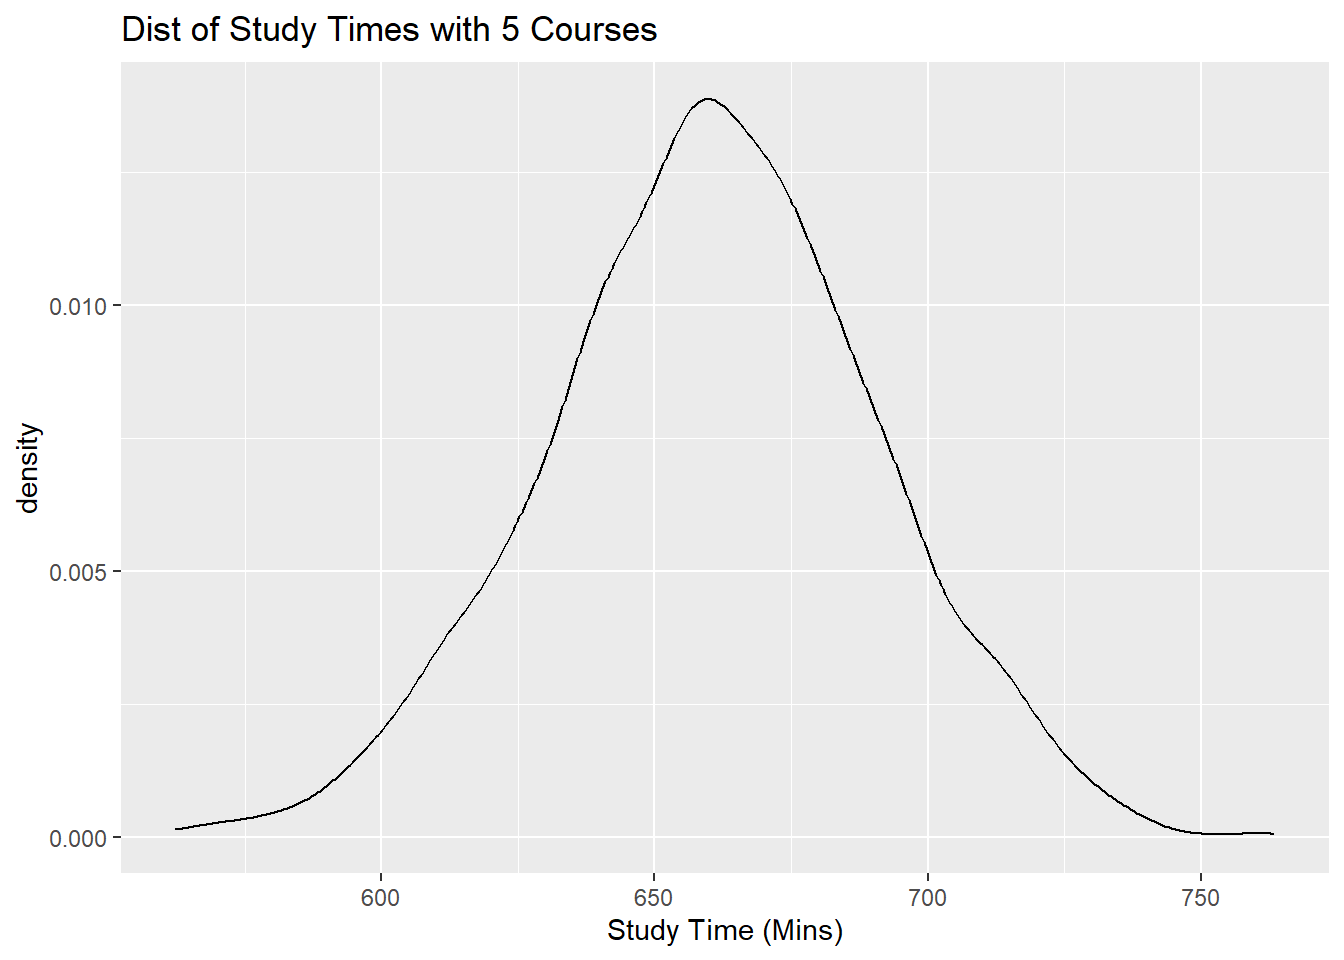
\includegraphics{bookdown-demo_files/figure-latex/unnamed-chunk-111-3.pdf}

Notice all of these plots are normal, with different means (centers), and similar spreads.

\emph{Please see the associated video for more explanation about the distribution of the response variable, for each value of the predictor variable, in an SLR setting.}

\hypertarget{estimating-regression-coefficients-in-slr}{%
\section{Estimating Regression Coefficients in SLR}\label{estimating-regression-coefficients-in-slr}}

From \eqref{eq:SLR} and \eqref{eq:SLRmod}, we noted that we have to estimate the regression coefficients \(\beta_0, \beta_1\) as well as the parameter \(\sigma^2\) associated with the error term. As mentioned earlier, we are unable to obtain numerical values of these parameters as we do not have data from the entire population. So what we do is use the data from our sample to estimate these parameters.

We estimate \(\beta_0,\beta_1\) using \(\hat{\beta}_0,\hat{\beta}_1\) based on a sample of observations \((x_i,y_i)\) of size \(n\).

The subscripts associated with the response and predictor variables denote which data point that value belongs to. Let us take a look at the first few rows of the data frame for the study time example:

\begin{Shaded}
\begin{Highlighting}[]
\FunctionTok{head}\NormalTok{(df)}
\end{Highlighting}
\end{Shaded}

\begin{verbatim}
##      study courses
## 1 429.8311       3
## 2 458.4588       3
## 3 391.9406       3
## 4 378.0196       3
## 5 397.9856       3
## 6 405.7145       3
\end{verbatim}

For example, \(x_1\) denotes the number of courses taken by student number 1 in the dataframe, which is 3. \(y_4\) denotes the study time for student number 4 in the dataframe, which is 378.0196456.

Following \eqref{eq:SLR} and \eqref{eq:SLRmod}, the sample versions are

\begin{equation} 
\hat{y}=\hat{\beta}_0+\hat{\beta}_1 x
\label{eq:fitted}
\end{equation}

and

\begin{equation} 
y=\hat{\beta}_0+\hat{\beta}_1 x + e
\label{eq:fitted-model}
\end{equation}

respectively. \eqref{eq:fitted} is called the \textbf{estimated SLR equation}, or \textbf{fitted SLR equation}. \eqref{eq:fitted-model} is called the \textbf{estimated SLR model}.

\(\hat{\beta}_1,\hat{\beta}_0\) are the estimators for \(\beta_1,\beta_0\) respectively. These estimators can be interpreted in the following manner:

\begin{itemize}
\tightlist
\item
  \textbf{\(\hat{\beta}_1\) denotes the change in the predicted \(y\) when \(x\) increases by 1 unit. Alternatively, it denotes the change in \(y\), on average, when \(x\) increases by 1 unit.}
\item
  \textbf{\(\hat{\beta}_0\) denotes the predicted \(y\) when \(x=0\). Alternatively, it denotes the average of \(y\) when \(x=0\).}
\end{itemize}

From \eqref{eq:fitted-model}, notice we use \textbf{\(e\) to denote the residual}, or in other words, the ``error'' in the sample.

From \eqref{eq:fitted} and \eqref{eq:fitted-model}, we have the following quantities that we can compute:

\begin{equation}
\text{Predicted/Fitted values: } \hat{y}_i = \hat{\beta}_0+\hat{\beta}_1 x_i.
\label{eq:fits}
\end{equation}

\begin{equation} 
\text{Residuals: } e_i = y_i-\hat{y}_i.
\label{eq:res}
\end{equation}

\begin{equation} 
\text{Sum of Squared Residuals: } SS_{res} =  \sum\limits_{i=1}^n(y_i-\hat{y}_i)^2.
\label{eq:SSres}
\end{equation}

We compute the estimated coefficients \(\hat{\beta}_1,\hat{\beta}_0\) using the \textbf{method of least squares}, i.e.~choose the numerical values of \(\hat{\beta}_1,\hat{\beta}_0\) that minimize \(SS_{res}\) as given in \eqref{eq:SSres}.

By minimizing \(SS_{res}\) with respect to \(\hat{\beta}_0\) and \(\hat{\beta}_1\), the estimated coefficients in the simple linear regression equation are

\begin{equation} 
\hat{\beta}_1 = \frac{\sum\limits_{i=1}^n(x_i-\bar{x})(y_i-\bar{y})}{\sum\limits_{i=1}^n(x_i-\bar{x})^2}
\label{eq:b1}
\end{equation}

and

\begin{equation} 
\hat{\beta}_0 = \bar{y}- \hat{\beta}_1 \bar{x}
\label{eq:b0}
\end{equation}

\(\hat{\beta}_1, \hat{\beta}_0\) are called \textbf{least squares estimators}.

The minimization of \(SS_{res}\) with respect to \(\hat{\beta}_0\) and \(\hat{\beta}_1\) is done by taking the partial derivatives of \eqref{eq:SSres} with respect to \(\hat{\beta}_1\) and \(\hat{\beta}_0\), setting these two partial derivatives equal to 0, and solving these two equations for \(\hat{\beta}_1\) and \(\hat{\beta}_0\).

Let's take a look at the estimated coefficients for our study time example:

\begin{Shaded}
\begin{Highlighting}[]
\DocumentationTok{\#\#fit regression}
\NormalTok{result}\OtherTok{\textless{}{-}}\FunctionTok{lm}\NormalTok{(study}\SpecialCharTok{\textasciitilde{}}\NormalTok{courses, }\AttributeTok{data=}\NormalTok{df)}
\DocumentationTok{\#\#print out the estimated coefficients}
\NormalTok{result}
\end{Highlighting}
\end{Shaded}

\begin{verbatim}
## 
## Call:
## lm(formula = study ~ courses, data = df)
## 
## Coefficients:
## (Intercept)      courses  
##       58.45       120.39
\end{verbatim}

From our sample of 6000 students, we have

\begin{itemize}
\tightlist
\item
  \(\hat{\beta}_1\) = 120.3930985. The predicted study time increases by 120.3930985 minutes for each additional course taken.
\item
  \(\hat{\beta}_0\) = 58.4482853. The predicted study time is 58.4482853 when no courses are taken. Notice this value does not make sense, as a student cannot be taking 0 courses. If you look at our data, the number of courses taken is 3, 4, or 5. So we should only use our regression when \(3 \leq x \leq 5\). We cannot use it for values of \(x\) outside the range of our data. Making predictions of the response variable for predictors outside the range of the data is called \textbf{extrapolation} and should not be done.
\end{itemize}

\hypertarget{estimating-variance-of-errors-in-slr}{%
\section{Estimating Variance of Errors in SLR}\label{estimating-variance-of-errors-in-slr}}

The estimator of \(\sigma^2\), the variance of the error terms (also the variance of the probability distribution of \(y\) given \(x\)) is
\begin{equation} 
s^2 = MS_{res} = \frac{SS_{res}}{n-2} = \frac{\sum\limits_{i=1}^n e_i^2}{n-2},
\label{eq:variance}
\end{equation}

where \(MS_{res}\) is the called the \textbf{mean squared residuals}.

\(\sigma^2\), the variance of the error terms, measures the spread of the response variable, for each value of \(x\). The smaller this is, the closer the data points are to the regression equation.

\hypertarget{practice-questions-1}{%
\subsection{Practice questions}\label{practice-questions-1}}

Take a look at the scatterplot of study time against number of courses taken, Figure \ref{fig:scatter-courses}. On this plot, label the following:

\begin{itemize}
\tightlist
\item
  estimated SLR equation
\item
  the fitted value when \(x=3\), \(x=4\), and \(x=5\).
\item
  the residual for any data point on the plot of your choosing.
\end{itemize}

\emph{Try these on your own first, then view the associated video to see if you labeled the plot correctly!}

\hypertarget{assessing-linear-association}{%
\section{Assessing Linear Association}\label{assessing-linear-association}}

As noted earlier, the variance of the error terms inform us how close the data points are to the estimated SLR equation. The smaller the variance of the error terms, the closer the data points are to the estimated SLR equation. This in turn implies the linear relationship between the variables is stronger.

We will learn about some common measures that are used to quantify the strength of the linear relationship between the response and predictor variables. Before we do that, we need to define some other terms.

\hypertarget{sum-of-squares}{%
\subsection{Sum of squares}\label{sum-of-squares}}

\begin{equation} 
\text{Total Sum of Squares: } SS_T = \sum\limits_{i=1}^{n} (y_i - \bar{y})^{2}.
\label{eq:SST}
\end{equation}

Total sum of squares is defined as the \textbf{total variance in the response variable}. The larger this value is, the larger the spread is of the response variable.

\begin{equation} 
\text{Regression sum of squares: } SS_R = \sum\limits_{i=1}^{n} (\hat{y_i} - \bar{y})^{2}.
\label{eq:SSR}
\end{equation}

Regression sum of squares is defined as the \textbf{variance in the response variable that can be explained by our regression}.

We also have residual sum of squares, \(SS_{res}\). Its mathematical formulation is given in \eqref{eq:SSres}. It is defined as the \textbf{variance in the response variable that cannot be explained by our regression}.

It can be shown that

\begin{equation}
SS_T = SS_R + SS_{res}.
\label{eq:SS}
\end{equation}

Each of the sums of squares has its associated \textbf{degrees of freedom (df)}:

\begin{itemize}
\tightlist
\item
  df for \(SS_R\): \(df_R = 1\)
\item
  df for \(SS_{res}\): \(df_{res} = n-2\)
\item
  df for \(SS_T\): \(df_T = n-1\)
\end{itemize}

\emph{Please see the associated video for more explanation about the concept behind degrees of freedom.}

\hypertarget{anova-table}{%
\subsection{ANOVA Table}\label{anova-table}}

Information regarding the sums of squares is usually presented in the form of an \textbf{ANOVA (analysis of variance) table}:

\begin{longtable}[]{@{}
  >{\centering\arraybackslash}p{(\columnwidth - 8\tabcolsep) * \real{0.2353}}
  >{\centering\arraybackslash}p{(\columnwidth - 8\tabcolsep) * \real{0.2941}}
  >{\centering\arraybackslash}p{(\columnwidth - 8\tabcolsep) * \real{0.1569}}
  >{\centering\arraybackslash}p{(\columnwidth - 8\tabcolsep) * \real{0.1569}}
  >{\centering\arraybackslash}p{(\columnwidth - 8\tabcolsep) * \real{0.1569}}@{}}
\toprule\noalign{}
\begin{minipage}[b]{\linewidth}\centering
Source of Variation
\end{minipage} & \begin{minipage}[b]{\linewidth}\centering
SS
\end{minipage} & \begin{minipage}[b]{\linewidth}\centering
df
\end{minipage} & \begin{minipage}[b]{\linewidth}\centering
MS
\end{minipage} & \begin{minipage}[b]{\linewidth}\centering
F
\end{minipage} \\
\midrule\noalign{}
\endhead
\bottomrule\noalign{}
\endlastfoot
Regression & \(SS_R=\sum\left(\hat{y_i}-\bar{y}\right)^2\) & \(df_R = 1\) & \(MS_R=\frac{SS_R}{df_R}\) & \(\frac{MS_R}{MS_{res}}\) \\
Error & \(SS_{res} = \sum\left(y_i-\hat{y_i}\right)^2\) & \(df_{res} = n-2\) & \(MS_{res}=\frac{SS_{res}}{df_{res}}\) & \texttt{***} \\
Total & \(SS_T=\sum\left(y_i-\bar{y}\right)^2\) & \(df_T = n-1\) & \texttt{***} & \texttt{***} \\
\end{longtable}

Note:

\begin{itemize}
\tightlist
\item
  Dividing each sum of square with its corresponding degrees of freedom gives the corresponding mean square.
\item
  In the last column, we report an \(F\) statistic, which equal to \(\frac{MS_R}{MS_{res}}\). This \(F\) statistic is associated with an \textbf{ANOVA F test}, which we will look at in more detail in the next subsection.
\end{itemize}

To obtain the ANOVA table for our study time example:

\begin{Shaded}
\begin{Highlighting}[]
\FunctionTok{anova}\NormalTok{(result)}
\end{Highlighting}
\end{Shaded}

\begin{verbatim}
## Analysis of Variance Table
## 
## Response: study
##             Df   Sum Sq  Mean Sq F value    Pr(>F)    
## courses      1 57977993 57977993   65404 < 2.2e-16 ***
## Residuals 5998  5317017      886                      
## ---
## Signif. codes:  0 '***' 0.001 '**' 0.01 '*' 0.05 '.' 0.1 ' ' 1
\end{verbatim}

Notice that R does not print out the information for the line regarding \(SS_T\).

\hypertarget{anova-f-test}{%
\subsection{\texorpdfstring{ANOVA \(F\) Test}{ANOVA F Test}}\label{anova-f-test}}

In SLR, the ANOVA \(F\) statistic from the ANOVA table can be used to test if the slope of the SLR equation is 0 or not. In words, this means that whether there is a linear association between the variables or not. If the slope is 0, it means that changes in the value of the predictor variable do not change the value of the response variable, on average; hence the variables are not linearly associated.

The null and alternative hypotheses are:

\[
H_0: \beta_1 = 0, H_a: \beta_1 \neq 0.
\]
The test statistic is

\begin{equation} 
F = \frac{MS_R}{MS_{res}}
\label{eq:ANOVA}
\end{equation}

and is compared with an \(F_{1,n-2}\) distribution. Note that \(F_{1,n-2}\) is read as an \textbf{F distribution with 1 and \(n-2\) degrees of freedom}.

Going back to the study time example, the \(F\) statistic is \ensuremath{6.5403586\times 10^{4}}. The critical value can be found using

\begin{Shaded}
\begin{Highlighting}[]
\FunctionTok{qf}\NormalTok{(}\DecValTok{1}\FloatTok{{-}0.05}\NormalTok{, }\DecValTok{1}\NormalTok{, }\DecValTok{6000{-}2}\NormalTok{)}
\end{Highlighting}
\end{Shaded}

\begin{verbatim}
## [1] 3.84301
\end{verbatim}

Since our test statistic is larger than the critical value, we reject the null hypothesis. Our data support the claim that the slope is different from 0, or in other words, that there is a linear association between study time and number of courses taken.

\hypertarget{coefficient-of-determination}{%
\subsection{Coefficient of determination}\label{coefficient-of-determination}}

The \textbf{coefficient of determination, \(R^2\),} is

\begin{equation}
R^{2} = \frac{SS_R}{SS_T} = 1 - \frac{SS_{res}}{SS_T}.
\label{eq:R2}
\end{equation}

\(R^{2}\) is an indication of how well the data fits our model. In the context of simple linear regression, it denotes \textbf{the proportion of variance in the response variable that is explained by the predictor}.

A few notes about \(R^2\):

\begin{itemize}
\tightlist
\item
  \(0 \leq R^2 \leq 1\).
\item
  Values closer to 1 indicate a better fit; values closer to 0 indicate a poorer fit.
\item
  Sometimes reported as a percentage.
\end{itemize}

To obtain \(R^2\) for our study time example:

\begin{Shaded}
\begin{Highlighting}[]
\NormalTok{anova.tab}\OtherTok{\textless{}{-}}\FunctionTok{anova}\NormalTok{(result)}
\DocumentationTok{\#\#SST not provided, so we add up SSR and SSres}
\NormalTok{SST}\OtherTok{\textless{}{-}}\FunctionTok{sum}\NormalTok{(anova.tab}\SpecialCharTok{$}\StringTok{"Sum Sq"}\NormalTok{)}
\DocumentationTok{\#\#R2}
\NormalTok{anova.tab}\SpecialCharTok{$}\StringTok{"Sum Sq"}\NormalTok{[}\DecValTok{1}\NormalTok{]}\SpecialCharTok{/}\NormalTok{SST}
\end{Highlighting}
\end{Shaded}

\begin{verbatim}
## [1] 0.9159963
\end{verbatim}

This implies that the proportion of variance in study time that can be explained by the number of courses taken is 0.9159963.

\hypertarget{correlation}{%
\subsection{Correlation}\label{correlation}}

A measure used to quantify the strength of the linear association between two quantitative variables is the \textbf{sample correlation}. The sample correlation, \(\mbox{Corr}(x,y)\) or \(r\), is given by

\begin{equation} 
r = \frac{\sum\limits_{i=1}^{n}(x_i - \bar{x})(y_i - \bar{y})}{\sqrt{\sum\limits_{i=1}^{n}(x_i - \bar{x})^{2}(y_i - \bar{y})^{2}}}.
\label{eq:corr}
\end{equation}

A few notes about \(r\):

\begin{itemize}
\tightlist
\item
  \(-1 \leq r \leq 1\).
\item
  Sign of correlation indicates direction of association. A positive value indicates a positive linear association: as the predictor variable increases, so does the response variable, on average. A negative value indicates a negative linear association: as the predictor variable increases, the response variable decreases, on average.
\item
  Values closer to 1 or -1 indicate a stronger linear association; values closer to 0 indicate a weaker linear association.
\item
  In SLR, it turns out that \(r^2 = R^2\).
\end{itemize}

Using our study time example, the correlation between study time and number of courses taken is

\begin{Shaded}
\begin{Highlighting}[]
\FunctionTok{cor}\NormalTok{(df}\SpecialCharTok{$}\NormalTok{study, df}\SpecialCharTok{$}\NormalTok{courses)}
\end{Highlighting}
\end{Shaded}

\begin{verbatim}
## [1] 0.9570769
\end{verbatim}

This value indicates a very strong and positive linear association between study time and number of courses taken (remember that this is simulated data and is not real).

\hypertarget{how-strong-is-strong}{%
\subsubsection{How strong is strong?}\label{how-strong-is-strong}}

A question that is often raised is how large should the magnitude of the sample correlation be for it to be considered strong? The answer is: it depends on the context. If you are conducting an experiment that is governed by scientific laws (e.g an experiment verifying Newton's 2nd law that \(F = ma\)), we should expect an extremely high correlation. A correlation of 0.9 in such an instance may be considered weak. The value of the correlation you have should be compared with correlations from similar studies in that domain to determine if it is strong or not.

\hypertarget{a-word-of-caution}{%
\section{A Word of Caution}\label{a-word-of-caution}}

To be able to use the measures we have learned (such as correlation, \(R^2\)) and to interpret the estimated regression coefficients, we must verify via a scatterplot that the association between the two variables is approximately linear. If we see a non linear pattern in the scatterplot, we should not use or interpret these values. We will learn how to remedy the situation if we see a non linear pattern in the scatterplot in module 5.

\emph{Please see the associated video for a demonstration on how not looking at the scatterplot can lead to misleading interpretations.}

\hypertarget{r-tutorial}{%
\section{R Tutorial}\label{r-tutorial}}

For this tutorial, we will work with the dataset \texttt{elmhurst} from the \texttt{openintro} package in R.

\begin{Shaded}
\begin{Highlighting}[]
\FunctionTok{library}\NormalTok{(tidyverse)}
\FunctionTok{library}\NormalTok{(openintro)}
\NormalTok{Data}\OtherTok{\textless{}{-}}\NormalTok{openintro}\SpecialCharTok{::}\NormalTok{elmhurst}
\end{Highlighting}
\end{Shaded}

Type \texttt{?openintro::elmhurst} to read the documentation for datasets in R. Always seek to understand the background of your data! The key pieces of information are:

\begin{itemize}
\tightlist
\item
  A random sample of 50 students (all freshman from the 2011 class at Elmhurst College).
\item
  Family income of the student (units are missing).
\item
  Gift aid, in \$1000s.
\end{itemize}

We want to explore how family income may be related to gift aid, in a simple linear regression framework.

\hypertarget{visualization}{%
\subsection*{Visualization}\label{visualization}}
\addcontentsline{toc}{subsection}{Visualization}

We should always verify with scatterplot that the relationship is (approximately) linear before proceeding with correlation and simple linear regression!

\begin{Shaded}
\begin{Highlighting}[]
\DocumentationTok{\#\#scatterplot of gift aid against family income}
\NormalTok{ggplot2}\SpecialCharTok{::}\FunctionTok{ggplot}\NormalTok{(Data, }\FunctionTok{aes}\NormalTok{(}\AttributeTok{x=}\NormalTok{family\_income,}\AttributeTok{y=}\NormalTok{gift\_aid))}\SpecialCharTok{+}
  \FunctionTok{geom\_point}\NormalTok{()}\SpecialCharTok{+}
  \FunctionTok{geom\_smooth}\NormalTok{(}\AttributeTok{method =} \StringTok{"lm"}\NormalTok{, }\AttributeTok{se=}\ConstantTok{FALSE}\NormalTok{)}\SpecialCharTok{+}
  \FunctionTok{labs}\NormalTok{(}\AttributeTok{x=}\StringTok{"Family Income"}\NormalTok{, }\AttributeTok{y=}\StringTok{"Gift Aid"}\NormalTok{, }\AttributeTok{title=}\StringTok{"Scatterplot of Gift Aid against Family"}\NormalTok{)}
\end{Highlighting}
\end{Shaded}

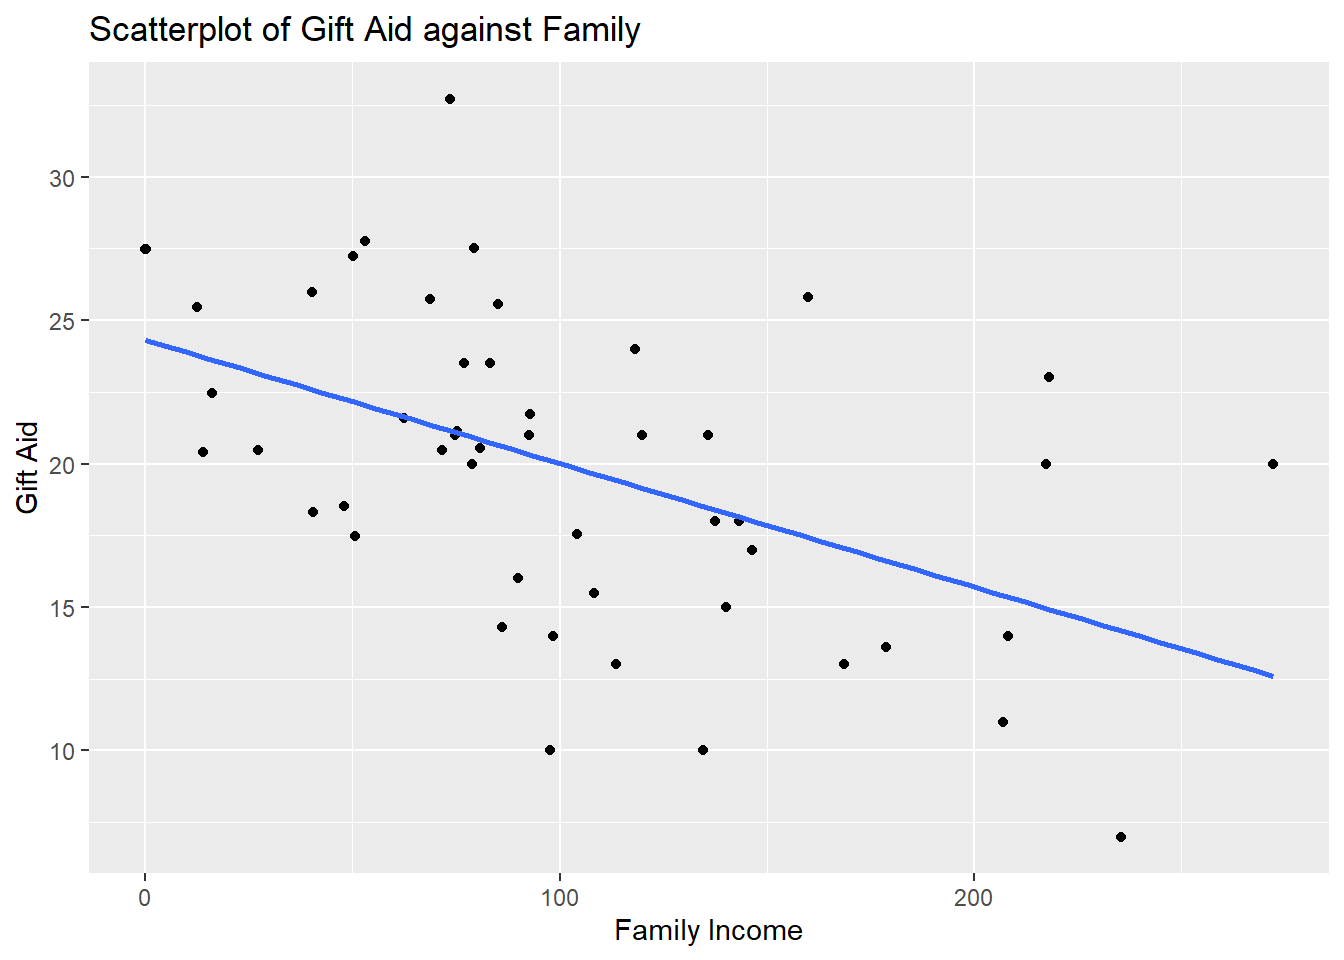
\includegraphics{bookdown-demo_files/figure-latex/unnamed-chunk-120-1.pdf}

We note that the observations are fairly evenly scattered on both sides of the regression line, so a linear association exists. We see a negative linear association. As family income increases, the gift aid, on average, decreases.

We also do not see any observation with weird values that may warrant further investigation.

\hypertarget{regression}{%
\subsection*{Regression}\label{regression}}
\addcontentsline{toc}{subsection}{Regression}

We use the \texttt{lm()} function to fit a regression model:

\begin{Shaded}
\begin{Highlighting}[]
\DocumentationTok{\#\#regress gift aid against family income}
\NormalTok{result}\OtherTok{\textless{}{-}}\FunctionTok{lm}\NormalTok{(gift\_aid}\SpecialCharTok{\textasciitilde{}}\NormalTok{family\_income, }\AttributeTok{data=}\NormalTok{Data)}
\end{Highlighting}
\end{Shaded}

Use the \texttt{summary()} function to display relevant information from this regression:

\begin{Shaded}
\begin{Highlighting}[]
\DocumentationTok{\#\#look at information regarding regression}
\FunctionTok{summary}\NormalTok{(result)}
\end{Highlighting}
\end{Shaded}

\begin{verbatim}
## 
## Call:
## lm(formula = gift_aid ~ family_income, data = Data)
## 
## Residuals:
##      Min       1Q   Median       3Q      Max 
## -10.1128  -3.6234  -0.2161   3.1587  11.5707 
## 
## Coefficients:
##               Estimate Std. Error t value Pr(>|t|)    
## (Intercept)   24.31933    1.29145  18.831  < 2e-16 ***
## family_income -0.04307    0.01081  -3.985 0.000229 ***
## ---
## Signif. codes:  0 '***' 0.001 '**' 0.01 '*' 0.05 '.' 0.1 ' ' 1
## 
## Residual standard error: 4.783 on 48 degrees of freedom
## Multiple R-squared:  0.2486, Adjusted R-squared:  0.2329 
## F-statistic: 15.88 on 1 and 48 DF,  p-value: 0.0002289
\end{verbatim}

We see the following values:

\begin{itemize}
\tightlist
\item
  \(\hat{\beta}_1 =\) -0.0430717. The estimated slope informs us the the predicted gift aid decreases by 0.0430717 thousands of dollars (or \$43.07) per unit increase in family income.
\item
  \(\hat{\beta}_0 =\) 24.319329. For students with no family income, their predicted gift aid is \$24 319.33. Note: from the scatterplot, we have an observation with 0 family income. We must be careful in not extrapolating when making predictions with our regression. We should only make predictions for family incomes between the minimum and maximum values of family incomes in our data.
\item
  \(s\) = 4.7825989, is the estimate of the standard deviation of the error terms. This is reported as residual standard error in R. Squaring this gives the estimated variance.
\item
  \(F\) = 15.8772043. This is the value of the ANOVA \(F\) statistic. The corresponding p-value is reported. Since this p-value is very small, we reject the null hypothesis. The data support the claim that there is a linear association between gift aid and family income.
\item
  \(R^2 =\) 0.2485582. The coefficient of determination informs us that about 24.86\% of the variation in gift aid can be explained by family income.
\end{itemize}

\hypertarget{extract-values-from-r-objects}{%
\subsubsection*{Extract values from R objects}\label{extract-values-from-r-objects}}
\addcontentsline{toc}{subsubsection}{Extract values from R objects}

We can actually extract these values that are being reported from \texttt{summary(result)}. To see what can be extracted from an R object, use the \texttt{names()} function:

\begin{Shaded}
\begin{Highlighting}[]
\DocumentationTok{\#\#see what can be extracted from summary(result)}
\FunctionTok{names}\NormalTok{(}\FunctionTok{summary}\NormalTok{(result))}
\end{Highlighting}
\end{Shaded}

\begin{verbatim}
##  [1] "call"          "terms"         "residuals"     "coefficients" 
##  [5] "aliased"       "sigma"         "df"            "r.squared"    
##  [9] "adj.r.squared" "fstatistic"    "cov.unscaled"
\end{verbatim}

To extract the estimated coefficients:

\begin{Shaded}
\begin{Highlighting}[]
\DocumentationTok{\#\#extract coefficients}
\FunctionTok{summary}\NormalTok{(result)}\SpecialCharTok{$}\NormalTok{coefficients}
\end{Highlighting}
\end{Shaded}

\begin{verbatim}
##                  Estimate Std. Error   t value     Pr(>|t|)
## (Intercept)   24.31932901 1.29145027 18.831022 8.281020e-24
## family_income -0.04307165 0.01080947 -3.984621 2.288734e-04
\end{verbatim}

Notice the information is presented in a table. To extract a specific value, we can specify the row and column indices:

\begin{Shaded}
\begin{Highlighting}[]
\DocumentationTok{\#\#extract slope}
\FunctionTok{summary}\NormalTok{(result)}\SpecialCharTok{$}\NormalTok{coefficients[}\DecValTok{2}\NormalTok{,}\DecValTok{1}\NormalTok{]}
\end{Highlighting}
\end{Shaded}

\begin{verbatim}
## [1] -0.04307165
\end{verbatim}

\begin{Shaded}
\begin{Highlighting}[]
\DocumentationTok{\#\#extract intercept}
\FunctionTok{summary}\NormalTok{(result)}\SpecialCharTok{$}\NormalTok{coefficients[}\DecValTok{1}\NormalTok{,}\DecValTok{1}\NormalTok{]}
\end{Highlighting}
\end{Shaded}

\begin{verbatim}
## [1] 24.31933
\end{verbatim}

On your own, extract the values of the residual standard error, the ANOVA F statistic, and \(R^2\).

\hypertarget{prediction}{%
\subsubsection*{Prediction}\label{prediction}}
\addcontentsline{toc}{subsubsection}{Prediction}

A use of regression models is prediction. Suppose I want to predict the gift aid of a student with family income of 50 thousand dollars (assuming the unit is in thousands of dollars). We use the \texttt{predict()} function:

\begin{Shaded}
\begin{Highlighting}[]
\DocumentationTok{\#\#create data point for prediction}
\NormalTok{newdata}\OtherTok{\textless{}{-}}\FunctionTok{data.frame}\NormalTok{(}\AttributeTok{family\_income=}\DecValTok{50}\NormalTok{)}
\DocumentationTok{\#\#predicted gift aid when x=50}
\FunctionTok{predict}\NormalTok{(result,newdata)}
\end{Highlighting}
\end{Shaded}

\begin{verbatim}
##        1 
## 22.16575
\end{verbatim}

This student's predicted gift aid is \$22 165.75. Alternatively, you could have calculated this by plugging \(x=50\) into the estimated SLR equation:

\begin{Shaded}
\begin{Highlighting}[]
\FunctionTok{summary}\NormalTok{(result)}\SpecialCharTok{$}\NormalTok{coefficients[}\DecValTok{1}\NormalTok{,}\DecValTok{1}\NormalTok{] }\SpecialCharTok{+} \FunctionTok{summary}\NormalTok{(result)}\SpecialCharTok{$}\NormalTok{coefficients[}\DecValTok{2}\NormalTok{,}\DecValTok{1}\NormalTok{]}\SpecialCharTok{*}\DecValTok{50}
\end{Highlighting}
\end{Shaded}

\begin{verbatim}
## [1] 22.16575
\end{verbatim}

\hypertarget{anova-table-1}{%
\subsubsection*{ANOVA table}\label{anova-table-1}}
\addcontentsline{toc}{subsubsection}{ANOVA table}

We use the \texttt{anova()} function to display the ANOVA table

\begin{Shaded}
\begin{Highlighting}[]
\NormalTok{anova.tab}\OtherTok{\textless{}{-}}\FunctionTok{anova}\NormalTok{(result)}
\NormalTok{anova.tab}
\end{Highlighting}
\end{Shaded}

\begin{verbatim}
## Analysis of Variance Table
## 
## Response: gift_aid
##               Df  Sum Sq Mean Sq F value    Pr(>F)    
## family_income  1  363.16  363.16  15.877 0.0002289 ***
## Residuals     48 1097.92   22.87                      
## ---
## Signif. codes:  0 '***' 0.001 '**' 0.01 '*' 0.05 '.' 0.1 ' ' 1
\end{verbatim}

The report \(F\) statistic is the same as the value reported earlier from \texttt{summary(result)}.

The first line of the output gives \(SS_{R}\), the second line gives \(SS_{res}\). The function doesn't provide \(SS_T\), but we know that \(SS_T = SS_{R} + SS_{res}\).

Again, to see what can be extracted from \texttt{anova.tab}:

\begin{Shaded}
\begin{Highlighting}[]
\FunctionTok{names}\NormalTok{(anova.tab)}
\end{Highlighting}
\end{Shaded}

\begin{verbatim}
## [1] "Df"      "Sum Sq"  "Mean Sq" "F value" "Pr(>F)"
\end{verbatim}

So \(SS_T\) can be easily calculated:

\begin{Shaded}
\begin{Highlighting}[]
\NormalTok{SST}\OtherTok{\textless{}{-}}\FunctionTok{sum}\NormalTok{(anova.tab}\SpecialCharTok{$}\StringTok{"Sum Sq"}\NormalTok{)}
\NormalTok{SST}
\end{Highlighting}
\end{Shaded}

\begin{verbatim}
## [1] 1461.079
\end{verbatim}

The \(R^2\) was reported to be 0.2485582. To verify using the ANOVA table:

\begin{Shaded}
\begin{Highlighting}[]
\NormalTok{anova.tab}\SpecialCharTok{$}\StringTok{"Sum Sq"}\NormalTok{[}\DecValTok{1}\NormalTok{]}\SpecialCharTok{/}\NormalTok{SST}
\end{Highlighting}
\end{Shaded}

\begin{verbatim}
## [1] 0.2485582
\end{verbatim}

\hypertarget{correlation-1}{%
\subsection*{Correlation}\label{correlation-1}}
\addcontentsline{toc}{subsection}{Correlation}

We use the \texttt{cor()} function to find the correlation between two quantitative variables:

\begin{Shaded}
\begin{Highlighting}[]
\DocumentationTok{\#\#correlation}
\FunctionTok{cor}\NormalTok{(Data}\SpecialCharTok{$}\NormalTok{family\_income,Data}\SpecialCharTok{$}\NormalTok{gift\_aid)}
\end{Highlighting}
\end{Shaded}

\begin{verbatim}
## [1] -0.4985561
\end{verbatim}

The correlation is -0.4985561. We have a moderate, negative linear association between family income and gift aid.

\hypertarget{inf}{%
\chapter{Inference with Simple Linear Regression (SLR)}\label{inf}}

\hypertarget{introduction-3}{%
\section{Introduction}\label{introduction-3}}

Oftentimes, the data we collect come from a random sample that is representative of the population of interest. A common example is an election poll before a presidential election. Random sampling allows the sample to be representative of the population. However, if we obtain another random sample, the characteristics of the new sample are unlikely to be exactly the same as the first sample. For example, the sample proportion who will vote for a certain party is unlikely to be the same for both random samples. What this tells us is that even with representative samples, sample proportions are unlikely to be equal to the population proportion, and sample proportions vary from sample to sample.

Dr.~W. Edwards Deming's Red Bead experiment illustrates this concept. A video of this experiment \href{https://www.youtube.com/watch?v=R3ewHrpqclA}{can be found here.}

In this video, the number of red beads, which represent bad products, varies each time the worker obtains a random sample of 50 beads. The fact that the number of red beads increases in his second sample does not indicate that he performed his task any worse, as this increase is due to the random variation associated with samples.

Note: Deming's Red Bead experiment was developed to illustrate concepts associated with management. He is best known for his work in developing the Japanese economy after World War II. You will be able to find many blogs/articles discussing the experiment on the World Wide Web. Although many of the articles discuss how this experiment applies in management, it can be used to illustrate concepts of variation.

The same idea extends to the slope and intercept of a regression line. The estimated slope and intercept will vary from sample to sample and are unlikely to be equal to the population slope and intercept. In inferential statistics, we use hypothesis tests and confidence intervals to aid us in accounting for this random variation. In this module, you will learn how to account for and quantify the random variation associated with the estimated regression model, and how to interpret the estimated regression model while accounting for random variation.

\hypertarget{review-from-previous-module}{%
\subsection{Review from previous module}\label{review-from-previous-module}}

The \textbf{simple linear regression model} is written as

\begin{equation}
y=\beta_0+\beta_{1} x + \epsilon. 
\label{eq:4SLRmod}
\end{equation}

We make some assumptions for the error term \(\epsilon\). They are:

\begin{enumerate}
\def\labelenumi{\arabic{enumi}.}
\tightlist
\item
  The errors have mean 0.
\item
  The \textbf{errors have variance denoted by \(\sigma^2\)}. Notice this variance is constant.
\item
  The errors are independent.
\item
  The errors are normally distributed.
\end{enumerate}

These assumptions allow us to derive the distributional properties associated with our least squares estimators \(\hat{\beta}_0, \hat{\beta}_1\), which then enables us to compute reliable confidence intervals and perform hypothesis tests on our SLR reliably.

\(\hat{\beta}_1,\hat{\beta}_0\) are the estimators for \(\beta_1,\beta_0\) respectively. These estimators can be interpreted in the following manner:

\begin{itemize}
\tightlist
\item
  \textbf{\(\hat{\beta}_1\) denotes the change in the predicted \(y\) when \(x\) increases by 1 unit. Alternatively, it denotes the change in \(y\), on average, when \(x\) increases by 1 unit.}
\item
  \textbf{\(\hat{\beta}_0\) denotes the predicted \(y\) when \(x=0\). Alternatively, it denotes the average of \(y\) when \(x=0\).}
\end{itemize}

How do the values of these estimators vary from sample to sample?

\hypertarget{hypothesis-testing-in-slr}{%
\section{Hypothesis Testing in SLR}\label{hypothesis-testing-in-slr}}

\hypertarget{distribution-of-least-squares-estimators}{%
\subsection{Distribution of least squares estimators}\label{distribution-of-least-squares-estimators}}

\textbf{Gauss Markov Theorem}: Under assumptions for a regression model, the least squares estimators \(\hat{\beta}_1\) and \(\hat{\beta}_0\) are unbiased and have minimum variance among all unbiased linear estimators.

Thus, the least squares estimators have the following properties:

\begin{enumerate}
\def\labelenumi{\arabic{enumi}.}
\tightlist
\item
  \(\mbox{E}(\hat{\beta}_1) = \beta_1\), \(\mbox{E}(\hat{\beta}_0) = \beta_0\)
\end{enumerate}

Note: An estimator is \textbf{unbiased} if its expected value is exactly equal to the parameter it is estimating.

\begin{enumerate}
\def\labelenumi{\arabic{enumi}.}
\setcounter{enumi}{1}
\tightlist
\item
  The variance of \(\hat{\beta}_1\) is
\end{enumerate}

\begin{equation} 
\mbox{Var}(\hat{\beta}_1) = \frac{\sigma^{2}}{\sum{(x_{i}-\bar{x})^{2}}}
\label{eq:4varb1}
\end{equation}

\begin{enumerate}
\def\labelenumi{\arabic{enumi}.}
\setcounter{enumi}{2}
\tightlist
\item
  The variance of \(\hat{\beta}_0\) is
\end{enumerate}

\begin{equation} 
\mbox{Var}(\hat{\beta}_0) = \sigma^2 \left[\frac{1}{n} + \frac{\bar{x}^2}{\sum (x_i -\bar{x})^2}\right]
\label{eq:4varb0}
\end{equation}

\begin{enumerate}
\def\labelenumi{\arabic{enumi}.}
\setcounter{enumi}{3}
\tightlist
\item
  \(\hat{\beta}_1\) and \(\hat{\beta}_0\) both follow a normal distribution.
\end{enumerate}

Note that in \eqref{eq:4varb1} and \eqref{eq:4varb0}, we use \(s^2 = MS_{res}\) to estimate \(\sigma^2\) since \(\sigma^2\) is a unknown value.

What these imply is that if we standardize \(\hat{\beta}_1\) and \(\hat{\beta}_0\), these standardized quantities will follow a \(t_{n-2}\) distribution, i.e.

\begin{equation} 
\frac{\hat{\beta}_1 - \beta_1}{se(\hat{\beta}_1)}\sim t_{n-2}
\label{eq:distb1}
\end{equation}

and

\begin{equation} 
\frac{\hat{\beta}_0 - \beta_0}{se(\hat{\beta}_0)}\sim t_{n-2},
\label{eq:distb0}
\end{equation}

where

\begin{equation}
se(\hat{\beta}_1) = \sqrt{\frac{MS_{res}}{\sum{(x_{i}-\bar{x})^{2}}}} = \frac{s}{\sqrt{\sum{(x_{i}-\bar{x})^{2}}}}
\label{eq:seb1}
\end{equation}

and

\begin{equation} 
se(\hat{\beta}_0) = \sqrt{MS_{res}\left[\frac{1}{n} + \frac{\bar{x}^2}{\sum (x_i -\bar{x})^2}\right]} = s \sqrt{\frac{1}{n} + \frac{\bar{x}^2}{\sum (x_i -\bar{x})^2}}
\label{eq:seb0}
\end{equation}

Note:

\begin{itemize}
\item
  \(se(\hat{\beta}_1)\) is read as the \textbf{standard error of \(\hat{\beta}_1\)}. The standard error of any estimator is essentially the sample standard deviation of that estimator, and measures the spread of that estimator.
\item
  A \(t_{n-2}\) distribution is read as a \textbf{\(t\) distribution with \(n-2\) degrees of freedom}.
\end{itemize}

\hypertarget{testing-regression-coefficients}{%
\subsection{Testing regression coefficients}\label{testing-regression-coefficients}}

Hypothesis testing is used to investigate if a population parameter is \textbf{different from a specific value}. In the context of SLR, we usually want to test if \(\beta_1\) is 0 or not. If \(\beta_1 = 0\), there is no linear relationship between the variables.

The general steps in hypothesis testing are:

\begin{itemize}
\tightlist
\item
  Step 1: State the null and alternative hypotheses.
\item
  Step 2: A test statistic is calculated using the sample, assuming the null is true. The value of the test statistic measures how the \textbf{sample deviates from the null}.
\item
  Step 3: Make conclusion, using either critical values or p-values.
\end{itemize}

In the previous module, we introduced the ANOVA \(F\) test. In SLR, this tests if the slope of the SLR equation is 0 or not. It turns out that we can also perform a \(t\) test for the slope. In the \(t\) test for the slope, the null and alternative hypotheses are:

\[
H_0: \beta_1 = 0, H_a: \beta_1 \neq 0.
\]
The test statistic is

\begin{equation} 
t = \frac{\hat{\beta}_1 - \text{ value in null}}{se(\hat{\beta}_1)}
\label{eq:4ttest}
\end{equation}

which is compared with a \(t_{n-2}\) distribution. Notice that \eqref{eq:4ttest} comes from \eqref{eq:distb1}.

Let us go back to our simulated example that we saw in the last module. We have data from 6000 UVa undergraduate students on the amount of time they spend studying in a week (in minutes), and how many courses they are taking in the semester (3 or 4 credit courses).

\begin{Shaded}
\begin{Highlighting}[]
\DocumentationTok{\#\#create dataframe}
\NormalTok{df}\OtherTok{\textless{}{-}}\FunctionTok{data.frame}\NormalTok{(study,courses)}

\DocumentationTok{\#\#fit regression}
\NormalTok{result}\OtherTok{\textless{}{-}}\FunctionTok{lm}\NormalTok{(study}\SpecialCharTok{\textasciitilde{}}\NormalTok{courses, }\AttributeTok{data=}\NormalTok{df)}
\DocumentationTok{\#\#look at regression coefficients}
\FunctionTok{summary}\NormalTok{(result)}\SpecialCharTok{$}\NormalTok{coefficients}
\end{Highlighting}
\end{Shaded}

\begin{verbatim}
##              Estimate Std. Error   t value      Pr(>|t|)
## (Intercept)  58.44829  1.9218752  30.41211 4.652442e-189
## courses     120.39310  0.4707614 255.74125  0.000000e+00
\end{verbatim}

The \(t\) statistic for testing \(H_0: \beta_1 = 0, H_a: \beta_1 \neq 0\) is reported to be 255.7412482, which can be calculated using \eqref{eq:4ttest}: \(t= \frac{120.39310 - 0}{0.4707614}\). The reported p-value is virtually 0, so we reject the null hypothesis. The data support the claim that there is a linear association between study time and the number of courses taken.

\hypertarget{confidence-intervals-for-regression-coefficients}{%
\section{Confidence Intervals for Regression Coefficients}\label{confidence-intervals-for-regression-coefficients}}

Confidence intervals (CIs) are similar to hypothesis testing in the sense that they are also based on the distributional properties of an estimator. CIs may differ in their use in the following ways:

\begin{enumerate}
\def\labelenumi{\arabic{enumi}.}
\tightlist
\item
  We are not assessing if the parameter is different from a specific value.
\item
  We are more interested in exploring a plausible \textbf{range of values for an unknown parameter}.
\end{enumerate}

Because CIs and hypothesis tests are based on the distributional properties of an estimator, their conclusions will be consistent (as long as the significance level is the same).

Recall the general form for CIs:

\begin{equation} 
\mbox{estimator} \pm (\mbox{multiplier} \times \mbox{s.e of estimator}). 
\label{eq:4CI}
\end{equation}

We have the following components of a CI

\begin{itemize}
\tightlist
\item
  \textbf{estimator (or statistic)}: numerical quantity that describes a sample
\item
  \textbf{multiplier}: determined by confidence level and relevant probability distribution
\item
  \textbf{standard error of estimator}: measure of variance of estimator (basically the square root of the variance of estimator)
\end{itemize}

Following \eqref{eq:4CI} and \eqref{eq:distb1}, the \(100(1-\alpha)\%\) CI for \(\beta_1\) is

\begin{equation} 
\hat{\beta}_1 \pm t_{1-\alpha/2;n-2}  se(\hat{\beta}_1) = \hat{\beta}_1 \pm t_{1-\alpha/2;n-2} \frac{s}{\sqrt{\sum(x_i - \bar{x})^{2}}}.
\label{eq:4CIb1}
\end{equation}

Going back to our study time example, the 95\% CI for \(\beta_1\) is (119.470237, 121.3159601).

\begin{Shaded}
\begin{Highlighting}[]
\DocumentationTok{\#\#CI for coefficients}
\FunctionTok{confint}\NormalTok{(result,}\AttributeTok{level =} \FloatTok{0.95}\NormalTok{)[}\DecValTok{2}\NormalTok{,]}
\end{Highlighting}
\end{Shaded}

\begin{verbatim}
##    2.5 %   97.5 % 
## 119.4702 121.3160
\end{verbatim}

An interpretation of this CI is that we have 95\% confidence that the true slope \(\beta_1\) lies between (119.470237, 121.3159601). In other words, for each additional course taken, the predicted study time increases between 119.470237 and 121.3159601 minutes.

\hypertarget{thought-questions}{%
\subsection{Thought questions}\label{thought-questions}}

\begin{itemize}
\item
  Is the conclusion from this 95\% CI consistent with the hypothesis test for \(H_0: \beta_1 = 0\) in the previous section at 0.05 significance level?
\item
  I have presented hypothesis tests and CIs for the slope, \(\beta_1\).

  \begin{itemize}
  \item
    How would you calculate the \(t\) statistic if you wanted to test \(H_0: \beta_0 = 0, H_0: \beta_0 \neq 0\)?
  \item
    How would you calculate the 95\% CI for the intercept \(\beta_0\)?
  \end{itemize}
\end{itemize}

Generally, we are usually more interested in the slope than the intercept.

\hypertarget{ci-of-the-mean-response}{%
\section{CI of the Mean Response}\label{ci-of-the-mean-response}}

We have established that the least squares estimators \(\hat{\beta}_1,\hat{\beta}_0\) have their associated variances. Since the estimated SLR equation is

\begin{equation} 
\hat{y}=\hat{\beta}_0+\hat{\beta}_1 x,
\label{eq:4fitted}
\end{equation}

it stands to reason that \(\hat{y}\) has an associated variance as well, since it is a function of \(\hat{\beta}_1,\hat{\beta}_0\).

There are two interpretations of \(\hat{y}\):

\begin{enumerate}
\def\labelenumi{\arabic{enumi}.}
\tightlist
\item
  it \textbf{estimates the mean of \(y\) when \(x=x_0\)};
\item
  it \textbf{predicts the value of \(y\) for a new observation when \(x=x_0\)}.
\end{enumerate}

Note: \(x_0\) denotes a specific numerical value for the predictor variable.

Depending on which interpretation we want, there are two different intervals based on \(\hat{y}\). The first interpretation is associated with the \textbf{confidence interval for the mean response, \(\hat{\mu}_{y|x_0}\), given the predictor}. This is used when we are interested in the average value of the response variable, when the predictor is equal to a specific value. This CI is

\begin{equation} 
\hat{\mu}_{y|x_0}\pm t_{1-\alpha/2,n-2}s\sqrt{\frac{1}{n} +
\frac{(x_0-\bar{x})^2}{\sum(x_i-\bar{x})^2}}.
\label{eq:4CImean}
\end{equation}

Going back to our study time example, suppose we want the average study time for students who take 5 courses, the 95\% CI is

\begin{Shaded}
\begin{Highlighting}[]
\DocumentationTok{\#\#CI for mean y when x=5}
\NormalTok{newdata}\OtherTok{\textless{}{-}}\FunctionTok{data.frame}\NormalTok{(}\AttributeTok{courses=}\DecValTok{5}\NormalTok{)}
\FunctionTok{predict}\NormalTok{(result, newdata, }\AttributeTok{level=}\FloatTok{0.95}\NormalTok{, }\AttributeTok{interval=}\StringTok{"confidence"}\NormalTok{)}
\end{Highlighting}
\end{Shaded}

\begin{verbatim}
##        fit      lwr      upr
## 1 660.4138 659.2224 661.6052
\end{verbatim}

We have 95\% confidence that the average study time for students who take 5 courses is between 659.2223688 and 661.605187 minutes.

\hypertarget{pi-of-a-new-response}{%
\section{PI of a New Response}\label{pi-of-a-new-response}}

Previously, we found a CI for the mean of \(y\) given a specific value of \(x\), \eqref{eq:4CImean}. This CI gives us an idea about the location of the regression line at a specific of \(x\).

Instead, we may have interest in finding an interval for a new value of \(\hat{y}_0\), when we have a new observation \(x=x_0\). This is called a \textbf{prediction interval (PI) for a future observation \(y_0\) when the predictor is a specific value}. This interval follows from the second interpretation of \(\hat{y}\).

The PI for \(\hat{y}_0\) takes into account:

\begin{enumerate}
\def\labelenumi{\arabic{enumi}.}
\tightlist
\item
  Variation in location for the distribution of \(y\) (i.e.~where is the center of the distribution of \(y\)?).
\item
  Variation \textbf{within the probability distribution of \(y\)}.
\end{enumerate}

By comparison, the confidence interval for the mean response \eqref{eq:4CImean} only takes into account the first element. The PI is

\begin{equation} 
\hat{y}_0\pm t_{1-\alpha/2,n-2}s \sqrt{1+\frac{1}{n} +
\frac{(x_0-\bar{x})^2}{\sum(x_i-\bar{x})^2}}.
\label{eq:4pred}
\end{equation}

Going back to our study time example, suppose we have a newly enrolled student who wishes to take 5 courses, and the student wants to predict his study time

\begin{Shaded}
\begin{Highlighting}[]
\DocumentationTok{\#\#PI for y when x=5}
\FunctionTok{predict}\NormalTok{(result, newdata, }\AttributeTok{level=}\FloatTok{0.95}\NormalTok{, }\AttributeTok{interval=}\StringTok{"prediction"}\NormalTok{)}
\end{Highlighting}
\end{Shaded}

\begin{verbatim}
##        fit      lwr      upr
## 1 660.4138 602.0347 718.7928
\end{verbatim}

We have 95\% confidence that the study time for this student is between 602.0347305 and 718.7928253 minutes.

\hypertarget{thought-questions-1}{%
\subsection{Thought questions}\label{thought-questions-1}}

\begin{itemize}
\item
  In the following two scenarios, decide if we are more interested in the CI for the mean response given the predictor \eqref{eq:4CImean}, or the PI for a future response given the predictor \eqref{eq:4pred}.

  \begin{itemize}
  \item
    We wish to estimate the waiting time, on average, of DMV customers if there are 10 people in line at the DMV.
  \item
    I enter the DMV and notice 10 people in line. I want to estimate my waiting time.
  \end{itemize}
\item
  Look at the standard errors associated with the intervals given in \eqref{eq:4CImean} and \eqref{eq:4pred}. How are they related to each other?
\end{itemize}

\hypertarget{supplemental-notes-on-statistical-inference}{%
\section{Supplemental Notes on Statistical Inference}\label{supplemental-notes-on-statistical-inference}}

\hypertarget{hypothesis-statements}{%
\subsection{Hypothesis statements}\label{hypothesis-statements}}

Let's consider a \(t\) test for the regression parameter, \(\beta_1\). Depending on context, the following could be null and alternative hypotheses

\begin{itemize}
\tightlist
\item
  \(H_0: \beta_1 = 0, H_a: \beta_1 \neq 0\).
\item
  \(H_0: \beta_1 = 0, H_a: \beta_1 > 0\).
\item
  \(H_0: \beta_1 = 0, H_a: \beta_1 < 0\).
\end{itemize}

The null hypothesis should be stated as a statement of \textbf{equality}. This concept holds true for hypothesis tests in general. Some other books / resources might state them as

\begin{itemize}
\tightlist
\item
  \(H_0: \beta_1 = 0, H_a: \beta_1 \neq 0\).
\item
  \(H_0: \beta_1 \leq 0, H_a: \beta_1 > 0\).
\item
  \(H_0: \beta_1 \geq 0, H_a: \beta_1 < 0\).
\end{itemize}

I prefer using the equality statement for the null hypothesis for the following reasons (theoretical, pedagogical, practical):

\begin{enumerate}
\def\labelenumi{\arabic{enumi}.}
\tightlist
\item
  The null hypothesis being an equality aligns with the definition of the p-value.
\end{enumerate}

\begin{itemize}
\tightlist
\item
  The p-value is the probability of observing our sample estimate (or a value more extreme), if the null hypothesis is true (i.e.~\(\beta_1\) is truly 0). This is what we are assuming in the calculation for the test statistic.
\end{itemize}

\begin{enumerate}
\def\labelenumi{\arabic{enumi}.}
\setcounter{enumi}{1}
\tightlist
\item
  People tend to get confused between the null and alternative hypotheses if both involve inequalities (the alternative is the hypothesis you are trying to support).
\item
  Conclusions are made in terms of supporting (or not supporting) the alternative hypothesis.
\end{enumerate}

\hypertarget{sample-size-and-statistical-inference}{%
\subsection{Sample size and statistical inference}\label{sample-size-and-statistical-inference}}

Generally speaking, there is a relationship between sample size and statistical inference (assuming other characteristics remain the same and our sample was randomly obtained or representative of the population of interest):

\begin{itemize}
\tightlist
\item
  Larger sample sizes (typically) lead to narrower confidence intervals (more precise intervals).
\item
  Sample estimates based on larger samples are more likely to be closer to the true parameters.
\item
  Larger sample (typically) lead to more evidence against the null hypothesis.

  \begin{itemize}
  \tightlist
  \item
    This means a larger sample size leads to a more powerful test. The power of a test is the probability a hypothesis test is able to correctly reject the null hypothesis.
  \end{itemize}
\end{itemize}

\hypertarget{small-sample-sizes}{%
\subsubsection{Small sample sizes}\label{small-sample-sizes}}

Small sample sizes tend to result in:

\begin{itemize}
\tightlist
\item
  Confidence intervals that are wide.
\item
  Sample estimates that are more likely to be further away from the true parameters.
\item
  Hypothesis tests that are more likely to incorrectly fail to reject the null hypothesis when the alternative hypothesis is true.
\end{itemize}

While larger sample sizes have their advantages, there are also some disadvantages with sample sizes that are extremely large.

\hypertarget{large-sample-sizes}{%
\subsubsection{Large sample sizes}\label{large-sample-sizes}}

A ``statistically significant'' result does not necessarily mean that the result has practical consequences. Suppose a 95\% confidence interval for \(\beta_1\) is \((0.001, 0.002)\). The interval excludes 0, so it is ``statistically significantly'' different from 0 (because it is!), but does this result have practical consequences? A narrow CI that barely excludes the null value can happen when we have a large sample size.

If one was to conduct the corresponding hypothesis test, we would reject the null hypothesis that \(\beta_1 = 0\). With large sample sizes, hypothesis tests are sensitive to small departures from the null hypothesis.

In such instances, it may be worth considering hypothesis tests involving a different value in the null hypothesis, one that makes sense for your question. For example, a practically significant slope may need to be greater than a specific numerical value for a certain context.

\begin{itemize}
\tightlist
\item
  Statistical inference to assess statistical significance.
\item
  Subject area knowledge to assess practical significance.
\end{itemize}

\hypertarget{questions}{%
\subsubsection{Questions}\label{questions}}

Are the following results statistically significant? If so, are the results also practically significant? Assume a two-sided test with a null value of 0 (These are made up examples):

\begin{enumerate}
\def\labelenumi{\arabic{enumi}.}
\item
  In assessing if studying more is associated with better test scores, a SLR is carried out with test scores (out of 100 points) against study time (in hours). The 95\% confidence interval for the slope \(\beta_1\) is (5.632, 7.829).
\item
  A SLR is carried out to explore the linear relationship between number of years in school with income (in thousands of dollars). The 95\% confidence interval for the slope \(\beta_1\) is (0.051, 0.243).
\end{enumerate}

\hypertarget{cautions-using-slr-and-correlation}{%
\subsection{Cautions using SLR and Correlation}\label{cautions-using-slr-and-correlation}}

Simple linear regression and correlation are meant for assessing \textbf{linear} relationships. If the relationship is not linear, we will need to transform the variable(s) (so the transformed variables have a linear relationship. Will explore this in Module \ref{diag}).

\begin{itemize}
\tightlist
\item
  Always verify via a scatterplot that the relationship is at least approximately linear.
\item
  A high correlation or a significant estimated slope by themselves do not prove that we have a strong linear relationship between the variables. Conversely, a correlation close to 0 or an insignificant estimated slope is also not proof that we do not have a relationship between the variables.
\end{itemize}

\hypertarget{outliers}{%
\subsubsection{Outliers}\label{outliers}}

SLR and correlation are sensitive to outliers / influential observations. Generally speaking, these are data that are ``far away'' or very different from the rest of the observations. These data points can be visually inspected from a scatterplot. Some potential considerations when dealing with such data points:

\begin{itemize}
\tightlist
\item
  Investigate these observations. There is usually something that is making them ``stand out'' from the rest of the data.
\item
  Data entry errors that can be corrected. Be sure to mention in the report.
\item
  Revisit how the data were sampled. Perhaps the data point is is not part of the population of interest. If so, data point can be removed (this is legitimate), but be sure to mention in the report.
\end{itemize}

With regards to regression analysis:

\begin{itemize}
\tightlist
\item
  Exclusion of data points must be clearly documented.
\item
  Fit the regression with and without the data points in question, and see how similar or different the conclusions become.
\item
  If the data points have large value(s) on the predictor and/or response, a log transformation on the variable can pull in the large values.
\item
  Consider subsetting your data and create separate models for each subset; or focus on a subset and make it clear your analysis is for a subset.
\item
  Knowing your data and context can help a lot in these decisions.
\end{itemize}

\hypertarget{association-and-causation}{%
\subsubsection{Association and causation}\label{association-and-causation}}

Two correlated variables do not mean that one variable causes the other variable to change. For example, consider a plot of ice cream consumption and deaths by drowning during various months. There may be some positive correlation, and clearly, eating more ice cream does not cause more drownings. The correlation can be explained by a third (lurking) variable: the weather.

A \textbf{lurking variable} is a variable that has an impact on the relationship between the variables being studied, but is itself not studied.

A carefully designed \textbf{randomized experiment} can control for lurking variables, and causal relationships can be established. Typically, such experiments include:

\begin{itemize}
\tightlist
\item
  A control group and a treatment group.
\item
  Random assignment of large number of observations into the treatment and control groups. Due to the random assignment, the general characteristics of of subjects in each group are similar.
\end{itemize}

Lurking variables are always an issue with \textbf{observational studies}. Researchers in observational studies do not intervene with the observations and simply observe the data that the observations generate. Causal relationships are much more difficult to establish with observational studies.

\hypertarget{questions-1}{%
\subsubsection{Questions}\label{questions-1}}

\begin{enumerate}
\def\labelenumi{\arabic{enumi}.}
\item
  Consider the \texttt{palmerpenguins} dataset that we have been working on. The data contain size measurements for three different species of penguins on three islands in the Palmer Archipelago, Antarctica over three years. Is this an observational study or randomized experiment?
\item
  A fertilizer company wishes to evaluate how effective a new fertilizer is in terms of improving the yield of crops. A large field is divided into many smaller plots, and each smaller plot is randomly assigned to receive either the new fertilizer or the standard fertilizer. Is this an observational study or randomized experiment?
\item
  A professor wishes to evaluate the effectiveness of various teaching methods (traditional vs flipped classroom). The professor uses the traditional approach for a section that meets on Mondays, Wednesdays, and Fridays from 9 to 10am and uses the flipped classroom approach for a section that meets on Mondays, Wednesdays, and Fridays from 2 to 3pm. Students were free to choose whichever section that wanted to register for, with no knowledge of the teaching method being used. What are some potential lurking variables in this study?
\end{enumerate}

\hypertarget{r-tutorial-1}{%
\section{R Tutorial}\label{r-tutorial-1}}

For this tutorial, we will continue to work with the dataset \texttt{elmhurst} from the \texttt{openintro} package in R.

\begin{Shaded}
\begin{Highlighting}[]
\FunctionTok{library}\NormalTok{(tidyverse)}
\FunctionTok{library}\NormalTok{(openintro)}
\NormalTok{Data}\OtherTok{\textless{}{-}}\NormalTok{openintro}\SpecialCharTok{::}\NormalTok{elmhurst}
\end{Highlighting}
\end{Shaded}

The key pieces of information are:

\begin{itemize}
\tightlist
\item
  A random sample of 50 students (all freshman from the 2011 class at Elmhurst College).
\item
  Family income of the student (units are missing).
\item
  Gift aid, in \$1000s.
\end{itemize}

We want to explore how family income may be related to gift aid, in a simple linear regression framework.

\hypertarget{hypothesis-test-for-beta_1-and-beta_0}{%
\subsection*{\texorpdfstring{Hypothesis test for \(\beta_1\) (and \(\beta_0\))}{Hypothesis test for \textbackslash beta\_1 (and \textbackslash beta\_0)}}\label{hypothesis-test-for-beta_1-and-beta_0}}
\addcontentsline{toc}{subsection}{Hypothesis test for \(\beta_1\) (and \(\beta_0\))}

Applying the \texttt{summary()} function to \texttt{lm()} gives the results of hypothesis tests for \(\beta_1\) and \(\beta_0\):

\begin{Shaded}
\begin{Highlighting}[]
\DocumentationTok{\#\#Fit a regression model}
\NormalTok{result}\OtherTok{\textless{}{-}}\FunctionTok{lm}\NormalTok{(gift\_aid}\SpecialCharTok{\textasciitilde{}}\NormalTok{family\_income, }\AttributeTok{data=}\NormalTok{Data)}

\DocumentationTok{\#\#look at t stats and F stat}
\FunctionTok{summary}\NormalTok{(result)}
\end{Highlighting}
\end{Shaded}

\begin{verbatim}
## 
## Call:
## lm(formula = gift_aid ~ family_income, data = Data)
## 
## Residuals:
##      Min       1Q   Median       3Q      Max 
## -10.1128  -3.6234  -0.2161   3.1587  11.5707 
## 
## Coefficients:
##               Estimate Std. Error t value Pr(>|t|)    
## (Intercept)   24.31933    1.29145  18.831  < 2e-16 ***
## family_income -0.04307    0.01081  -3.985 0.000229 ***
## ---
## Signif. codes:  0 '***' 0.001 '**' 0.01 '*' 0.05 '.' 0.1 ' ' 1
## 
## Residual standard error: 4.783 on 48 degrees of freedom
## Multiple R-squared:  0.2486, Adjusted R-squared:  0.2329 
## F-statistic: 15.88 on 1 and 48 DF,  p-value: 0.0002289
\end{verbatim}

Under coefficients, we can see the results of the hypothesis tests for \(\beta_1\) and \(\beta_0\). Specifically, for \(\beta_1\):

\begin{itemize}
\tightlist
\item
  \(\hat{\beta}_1\) = -0.0430717
\item
  \(se(\hat{\beta}_1)\) = 0.0108095
\item
  the test statistic is \(t\) = -3.984621
\item
  the corresponding p-value is \ensuremath{2.2887345\times 10^{-4}}
\end{itemize}

You can work out the p-value using R (slight difference due to rounding):

\begin{Shaded}
\begin{Highlighting}[]
\DocumentationTok{\#\#pvalue}
\DecValTok{2}\SpecialCharTok{*}\FunctionTok{pt}\NormalTok{(}\SpecialCharTok{{-}}\FunctionTok{abs}\NormalTok{(}\SpecialCharTok{{-}}\FloatTok{3.985}\NormalTok{), }\AttributeTok{df =} \DecValTok{50{-}2}\NormalTok{)}
\end{Highlighting}
\end{Shaded}

\begin{verbatim}
## [1] 0.0002285996
\end{verbatim}

Or find the critical value using R:

\begin{Shaded}
\begin{Highlighting}[]
\DocumentationTok{\#\#critical value}
\FunctionTok{qt}\NormalTok{(}\DecValTok{1}\FloatTok{{-}0.05}\SpecialCharTok{/}\DecValTok{2}\NormalTok{, }\AttributeTok{df =} \DecValTok{50{-}2}\NormalTok{)}
\end{Highlighting}
\end{Shaded}

\begin{verbatim}
## [1] 2.010635
\end{verbatim}

Either way, we end up rejecting the null hypothesis. The data support the claim that there is a linear association between gift aid and family income.

Note:

\begin{itemize}
\item
  the \(t\) tests for regression coefficients are based on \(H_0: \beta_j = 0, H_a: \beta_j \neq 0\). The reported p-value is based on this set of null and alternative hypotheses. If your null and alternative hypotheses are different, you will need to compute your own test statistic and p-value.
\item
  For SLR, the two-sided \(t\) test for \(\beta_1\) gives the exact same result as the ANOVA \(F\) test. Notice the p-values are the same. The \(F\) statistic of \(15.88\) is the squared of the \(t\) statistic, \((-3.985)^2\).
\end{itemize}

\hypertarget{confidence-interval-for-beta_1-and-beta_0}{%
\subsection*{\texorpdfstring{Confidence interval for \(\beta_1\) (and \(\beta_0\))}{Confidence interval for \textbackslash beta\_1 (and \textbackslash beta\_0)}}\label{confidence-interval-for-beta_1-and-beta_0}}
\addcontentsline{toc}{subsection}{Confidence interval for \(\beta_1\) (and \(\beta_0\))}

To find the 95\% confidence intervals for the coefficients, we use the \texttt{confint()} function:

\begin{Shaded}
\begin{Highlighting}[]
\DocumentationTok{\#\#to produce 95\% CIs for all regression coefficients}
\FunctionTok{confint}\NormalTok{(result,}\AttributeTok{level =} \FloatTok{0.95}\NormalTok{)}
\end{Highlighting}
\end{Shaded}

\begin{verbatim}
##                     2.5 %      97.5 %
## (Intercept)   21.72269421 26.91596380
## family_income -0.06480555 -0.02133775
\end{verbatim}

The 95\% CI for \(\beta_1\) is (-0.0648056, -0.0213378). We have 95\% confidence that for each additional thousand dollars in family income, the predicted gift aid decreases between \$21.3378 and \$64.8056.

\hypertarget{confidence-interval-for-mean-response-for-given-x}{%
\subsection*{Confidence interval for mean response for given x}\label{confidence-interval-for-mean-response-for-given-x}}
\addcontentsline{toc}{subsection}{Confidence interval for mean response for given x}

Suppose we want a confidence interval for the average gift aid for Elmhurst College students with family income of 80 thousand dollars. We can use the \texttt{predict()} function:

\begin{Shaded}
\begin{Highlighting}[]
\DocumentationTok{\#\#to produce 95\% CI for the mean response when x=80, }
\NormalTok{newdata}\OtherTok{\textless{}{-}}\FunctionTok{data.frame}\NormalTok{(}\AttributeTok{family\_income=}\DecValTok{80}\NormalTok{)}
\FunctionTok{predict}\NormalTok{(result,newdata,}\AttributeTok{level=}\FloatTok{0.95}\NormalTok{, }\AttributeTok{interval=}\StringTok{"confidence"}\NormalTok{)}
\end{Highlighting}
\end{Shaded}

\begin{verbatim}
##       fit      lwr      upr
## 1 20.8736 19.43366 22.31353
\end{verbatim}

The 95\% CI for the mean gift aid for students with family income of 80 thousand dollars is (19.4336609, 22.3135327). We have 95\% confidence the mean gift aid for students with family income of 80 thousand dollars is between \$19 433.66 and \$22 313.53.

\hypertarget{prediction-interval-for-a-response-for-a-given-x}{%
\subsection*{Prediction interval for a response for a given x}\label{prediction-interval-for-a-response-for-a-given-x}}
\addcontentsline{toc}{subsection}{Prediction interval for a response for a given x}

For a prediction interval for the gift aid of an Elmhurst College student with family income of 80 thousand dollars:

\begin{Shaded}
\begin{Highlighting}[]
\DocumentationTok{\#\#and the 95\% PI for the response of an observation when x=80}
\FunctionTok{predict}\NormalTok{(result,newdata,}\AttributeTok{level=}\FloatTok{0.95}\NormalTok{, }\AttributeTok{interval=}\StringTok{"prediction"}\NormalTok{)}
\end{Highlighting}
\end{Shaded}

\begin{verbatim}
##       fit      lwr      upr
## 1 20.8736 11.15032 30.59687
\end{verbatim}

We have 95\% confidence that for an Elmhurst College student with family income of 80, this student's gift aid is between \$11 150.32 and \$30 596.87.

\hypertarget{visualization-of-ci-for-mean-response-given-x-and-pi-of-response-given-x}{%
\subsection*{Visualization of CI for mean response given x and PI of response given x}\label{visualization-of-ci-for-mean-response-given-x-and-pi-of-response-given-x}}
\addcontentsline{toc}{subsection}{Visualization of CI for mean response given x and PI of response given x}

When using the \texttt{ggplot()} function to create a scatterplot, we can overlay the SLR equation by adding a layer via \texttt{geom\_smooth(method\ =\ lm)}. By default, the CI for the mean response for each value of the predictor gets overlaid as well. In the previous tutorial, we removed this by adding \texttt{se=FALSE} inside \texttt{geom\_smooth()}:

\begin{Shaded}
\begin{Highlighting}[]
\DocumentationTok{\#\#regular scatterplot}
\DocumentationTok{\#\#with regression line overlaid, and bounds of CI for mean y}
\NormalTok{ggplot2}\SpecialCharTok{::}\FunctionTok{ggplot}\NormalTok{(Data, }\FunctionTok{aes}\NormalTok{(}\AttributeTok{x=}\NormalTok{family\_income, }\AttributeTok{y=}\NormalTok{gift\_aid))}\SpecialCharTok{+}
  \FunctionTok{geom\_point}\NormalTok{() }\SpecialCharTok{+}
  \FunctionTok{geom\_smooth}\NormalTok{(}\AttributeTok{method=}\NormalTok{lm)}\SpecialCharTok{+}
  \FunctionTok{labs}\NormalTok{(}\AttributeTok{x=}\StringTok{"Family Income"}\NormalTok{, }
       \AttributeTok{y=}\StringTok{"Gift Aid"}\NormalTok{, }
       \AttributeTok{title=}\StringTok{"Scatterplot of Gift Aid against Family Income"}\NormalTok{)}
\end{Highlighting}
\end{Shaded}

\begin{verbatim}
## `geom_smooth()` using formula = 'y ~ x'
\end{verbatim}

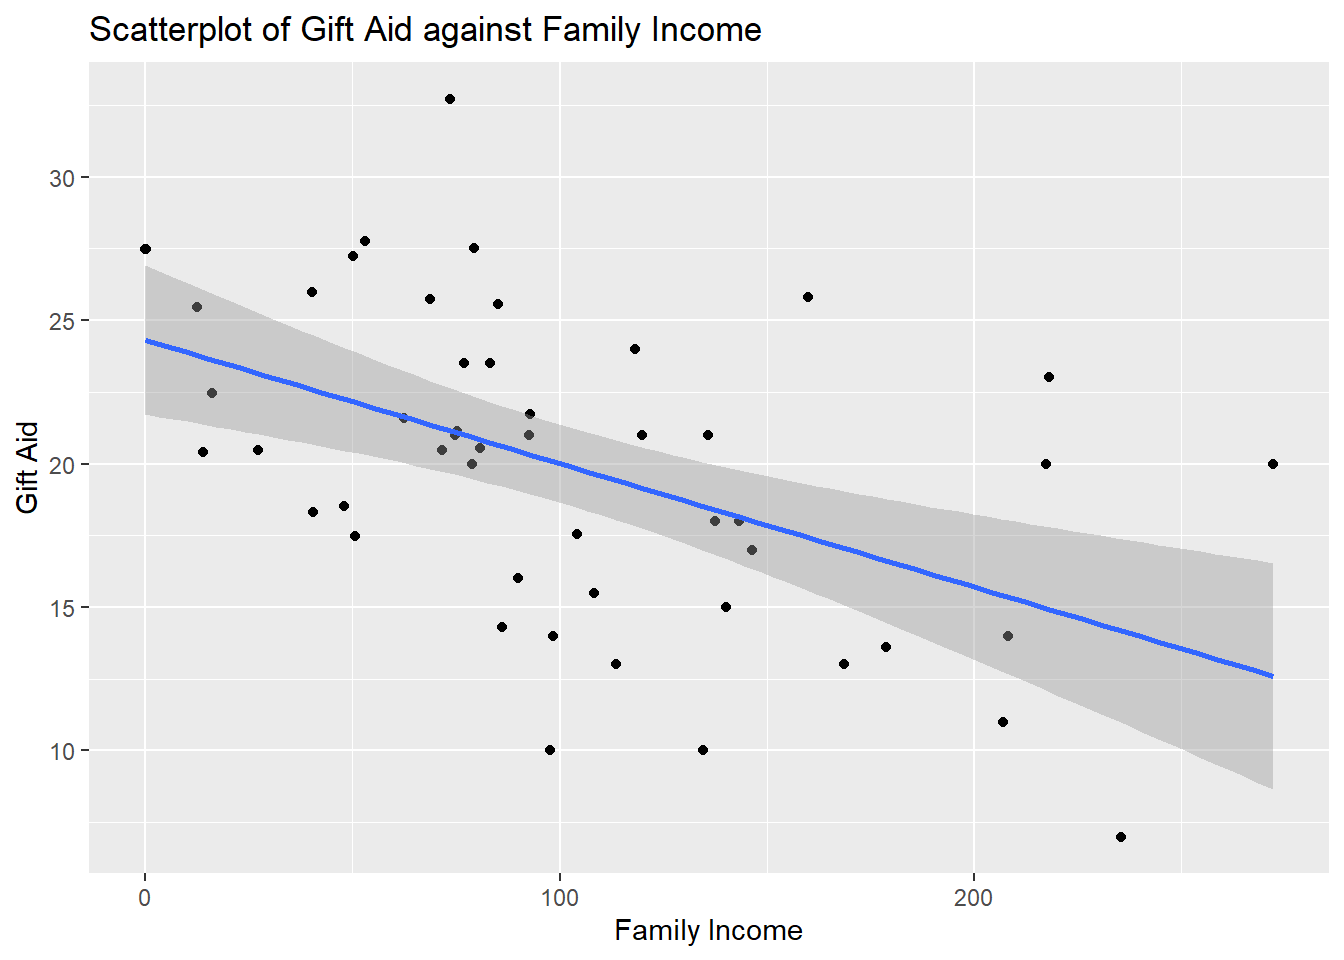
\includegraphics{bookdown-demo_files/figure-latex/unnamed-chunk-147-1.pdf}

Overlaying prediction intervals require a bit more work. We need to compute the lower and upper bounds of the PI for each value of the predictor:

\begin{Shaded}
\begin{Highlighting}[]
\DocumentationTok{\#\#find PIs for each observation}
\NormalTok{preds }\OtherTok{\textless{}{-}} \FunctionTok{predict}\NormalTok{(result, }\AttributeTok{interval=}\StringTok{"prediction"}\NormalTok{)}
\end{Highlighting}
\end{Shaded}

\begin{verbatim}
## Warning in predict.lm(result, interval = "prediction"): predictions on current data refer to _future_ responses
\end{verbatim}

Previously, when we used the \texttt{predict()} function, we provided the numerical value of \(x\) to make a prediction on. If this is not supplied, the function will use all the current values of \(x\) to make predictions, and will actually print out a warning message. For our purpose, this is not an issue since this is exactly what we want.

We then add \texttt{preds} to the data frame in order to overlay the lower and upper bounds on the scatterplot, by adding extra layers via \texttt{geom\_line()} in the \texttt{ggplot()} function:

\begin{Shaded}
\begin{Highlighting}[]
\DocumentationTok{\#\#add preds to data frame}
\NormalTok{Data}\OtherTok{\textless{}{-}}\FunctionTok{data.frame}\NormalTok{(Data,preds)}

\DocumentationTok{\#\#overlay PIs via geom\_line()}
\NormalTok{ggplot2}\SpecialCharTok{::}\FunctionTok{ggplot}\NormalTok{(Data, }\FunctionTok{aes}\NormalTok{(}\AttributeTok{x=}\NormalTok{family\_income, }\AttributeTok{y=}\NormalTok{gift\_aid))}\SpecialCharTok{+}
  \FunctionTok{geom\_point}\NormalTok{() }\SpecialCharTok{+}
  \FunctionTok{geom\_line}\NormalTok{(}\FunctionTok{aes}\NormalTok{(}\AttributeTok{y=}\NormalTok{lwr), }\AttributeTok{color =} \StringTok{"red"}\NormalTok{, }\AttributeTok{linetype =} \StringTok{"dashed"}\NormalTok{)}\SpecialCharTok{+}
  \FunctionTok{geom\_line}\NormalTok{(}\FunctionTok{aes}\NormalTok{(}\AttributeTok{y=}\NormalTok{upr), }\AttributeTok{color =} \StringTok{"red"}\NormalTok{, }\AttributeTok{linetype =} \StringTok{"dashed"}\NormalTok{)}\SpecialCharTok{+}
  \FunctionTok{geom\_smooth}\NormalTok{(}\AttributeTok{method=}\NormalTok{lm)}\SpecialCharTok{+}
  \FunctionTok{labs}\NormalTok{(}\AttributeTok{x=}\StringTok{"Family Income"}\NormalTok{, }
       \AttributeTok{y=}\StringTok{"Gift Aid"}\NormalTok{, }
       \AttributeTok{title=}\StringTok{"Scatterplot of Gift Aid against Family Income"}\NormalTok{)}
\end{Highlighting}
\end{Shaded}

\begin{verbatim}
## `geom_smooth()` using formula = 'y ~ x'
\end{verbatim}

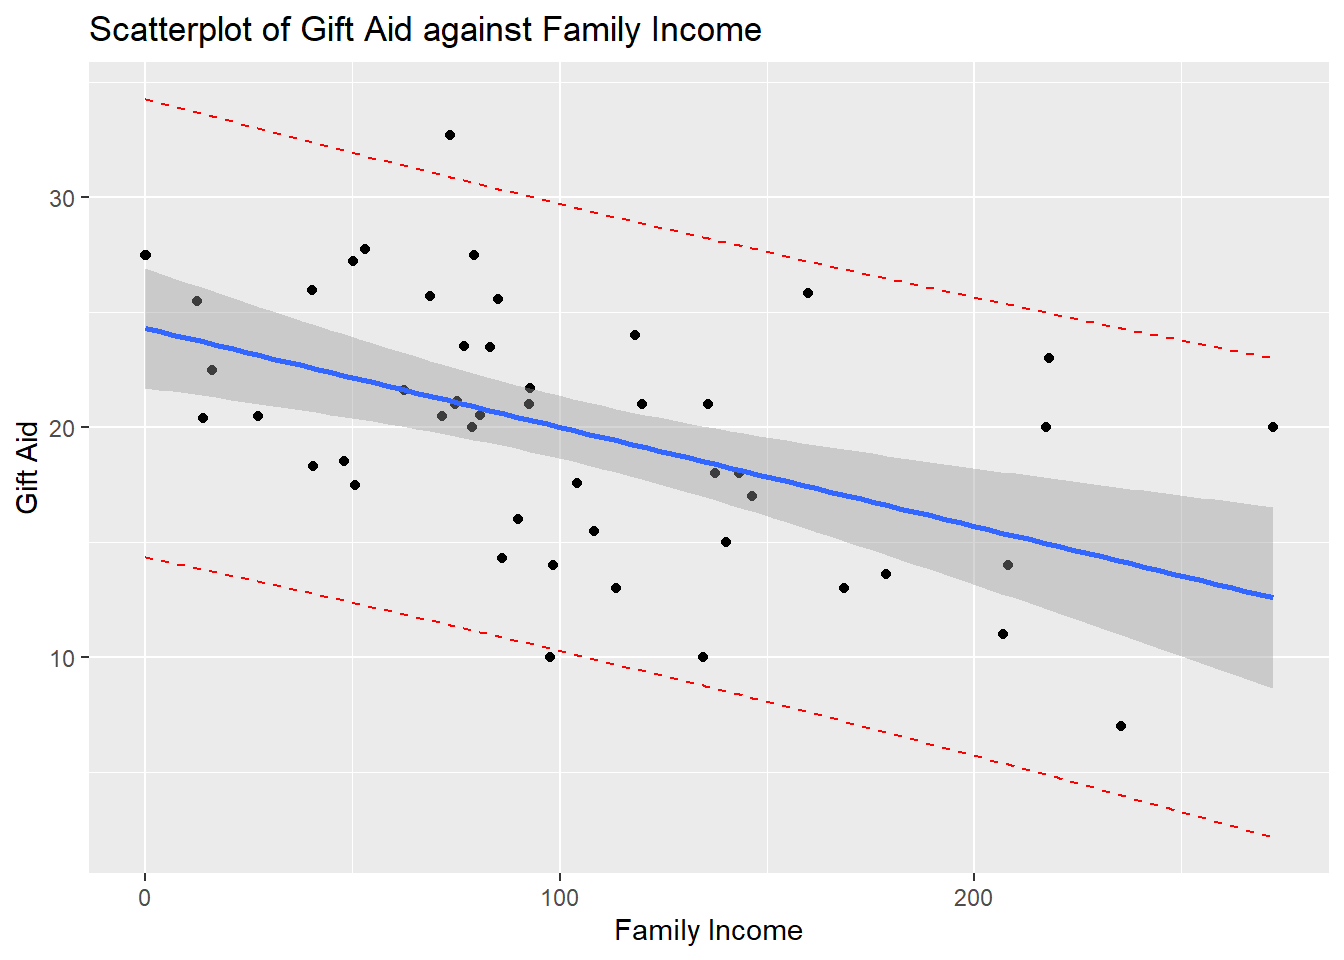
\includegraphics{bookdown-demo_files/figure-latex/unnamed-chunk-149-1.pdf}

As mentioned in the notes, the CI captures the location of the regression line, whereas the PI captures the data points.

\hypertarget{diag}{%
\chapter{Model Diagnostics and Remedial Measures in SLR}\label{diag}}

\hypertarget{introduction-4}{%
\section{Introduction}\label{introduction-4}}

The regression model is based on a number of assumptions. Those assumptions are made so that we can apply commonly used probability distributions to we quantify the variability associated with our estimated regression model. This means that if the assumptions are not met for our regression model, then how we quantify the variability associated with our model is no longer reliable. All our analysis with statistical inference becomes questionable.

In this module, you will learn how to assess whether the regression assumptions are met. We will explore ways in which we can transform our variables after diagnosing which assumptions are not met so that we can still proceed to build our regression model.

\hypertarget{assumptions-in-linear-regression}{%
\section{Assumptions in Linear Regression}\label{assumptions-in-linear-regression}}

In module \ref{slr}, we stated the SLR model as

\begin{equation} 
y=\beta_0+\beta_{1} x + \epsilon. 
\label{eq:5SLRmod}
\end{equation}

where \(f(x) = \beta_0 + \beta_1 x\). We need to make some assumptions for the error term \(\epsilon\). Mathematically, the assumptions are expressed as

\begin{equation} 
\epsilon_1,\ldots,\epsilon_n \ i.i.d. \sim N(0,\sigma^2)
\label{eq:5assumptions}
\end{equation}

Breaking down \eqref{eq:5assumptions} the assumptions can be expressed as the following:

\begin{enumerate}
\def\labelenumi{\arabic{enumi}.}
\tightlist
\item
  The errors have \textbf{mean 0}.
\item
  The errors have \textbf{constant variance denoted by \(\sigma^2\)}.
\item
  The errors are \textbf{independent}.
\item
  The errors are \textbf{normally distributed}.
\end{enumerate}

Let's dig a little deeper into the meaning and implications of these 4 assumptions.

\hypertarget{assumption-1-errors-have-mean-0.}{%
\subsection{Assumption 1: Errors have mean 0.}\label{assumption-1-errors-have-mean-0.}}

For each value of the predictor, the errors have \textbf{mean 0}. A by-product of this statement is that the relationship between \(y\) and \(x\), as expressed via \(y \approx f(x)\), is correct. So, if \(f(x) = \beta_0 + \beta_1 x\), then the relationship is approximately linear.

The plots in Figure \ref{fig:ass1} are based on simulated data. The scatterplot shown in Figure \ref{fig:ass1}(a) is an example of when this assumption is met. As we move from left to right on the plot, the data points are generally evenly scattered on both sides of the regression line that is overlaid.

\begin{figure}
\centering
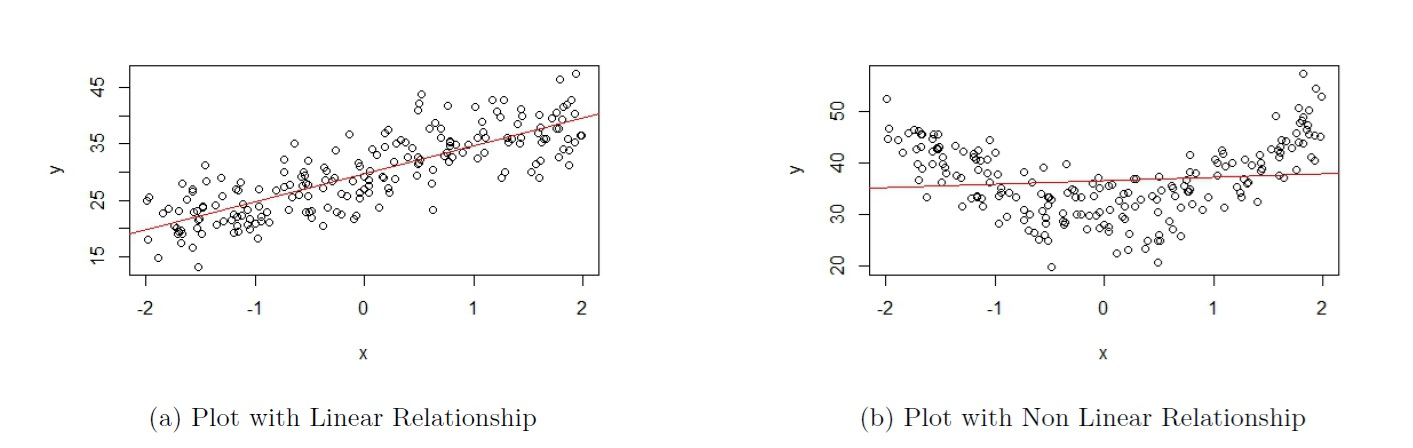
\includegraphics{images/ass1.jpg}
\caption{\label{fig:ass1}Assumption 1}
\end{figure}

The scatterplot shown in Figure \ref{fig:ass1}(b) is an example of when this assumption is \textbf{not} met. As we move from left to right on the plot in Figure \ref{fig:ass1}(b), the data points are generally not evenly scattered on both sides of the regression line that is overlaid.

\begin{itemize}
\tightlist
\item
  When \(-2 \leq x \leq -1.2\), the data points are generally above the regression line;
\item
  then when \(-1.2 < x < 1\), the data points are generally below the regression line;
\item
  and then when \(x \geq 1\), the data points are generally above the regression line.
\end{itemize}

\emph{Please see the associated video for more explanation on how to use Figure \ref{fig:ass1} to assess assumption 1.}

\hypertarget{consequences-of-violating-this-assumption}{%
\subsubsection{Consequences of violating this assumption}\label{consequences-of-violating-this-assumption}}

\textbf{Predictions will be biased}. This means that predicted values will systematically over- or under- estimate the true values of the response variable. Of the 4 assumptions listed, this is \textbf{most crucial assumption}.

Using Figure \ref{fig:ass1}(b) as an example, this implies that

\begin{itemize}
\tightlist
\item
  when \(-2 \leq x \leq -1.2\), the regression line will systematically under-predict the response variable;
\item
  then when \(-1.2 < x < 1\), the regression line will systematically over-predict the response variable;
\item
  and then when \(x \geq 1\), the regression line will systematically under-predict the response variable.
\end{itemize}

\hypertarget{assumption-2-errors-have-constant-variance}{%
\subsection{Assumption 2: Errors have constant variance}\label{assumption-2-errors-have-constant-variance}}

For each value of the predictor, the error terms have \textbf{constant variance}, denoted by \(\sigma^2\). This implies that when looking at a scatterplot, the vertical variation of data points around the regression equation has the same magnitude everywhere.

The plots in Figure \ref{fig:ass2} are based on simulated data. The scatterplot shown in Figure \ref{fig:ass2}(a) is an example of when this assumption is met (this figure is actually the same as Figure \ref{fig:ass1}(a), so the data that produced these plots satisfy both assumptions). As we move from left to right on the plot, the vertical variation of the data points about the regression line is approximately constant.

\begin{figure}
\centering
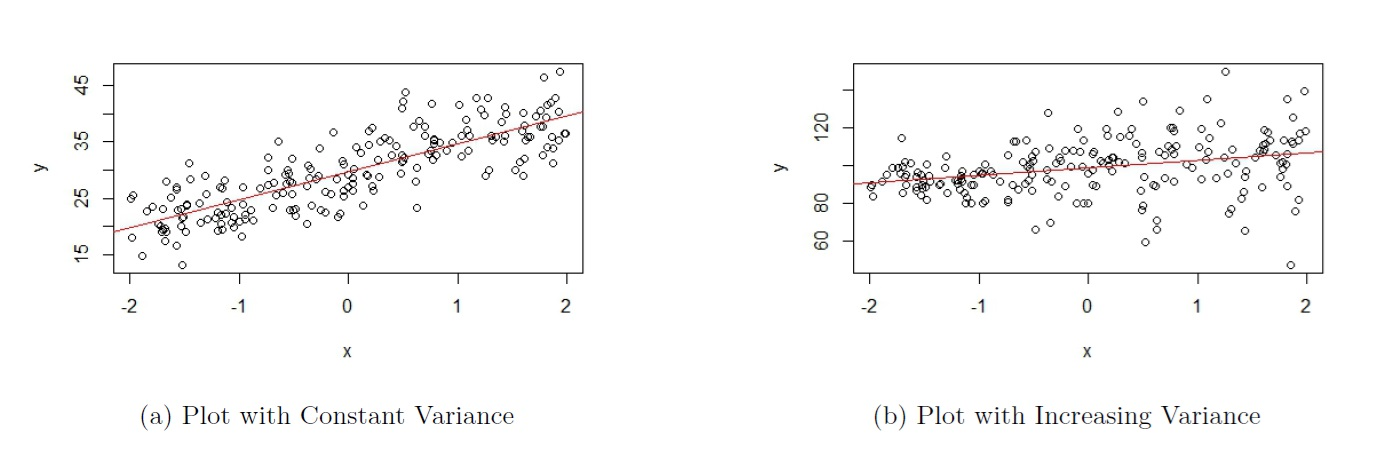
\includegraphics{images/ass2.jpg}
\caption{\label{fig:ass2}Assumption 2}
\end{figure}

The scatterplot shown in Figure \ref{fig:ass2}(b) is an example of when this assumption is \textbf{not} met. As we move from left to right on the plot in Figure \ref{fig:ass2}(b), the vertical variation of the data points about the regression line becomes larger as the value of the response variable gets larger, so the variance is not constant.

\emph{Please see the associated video for more explanation on how to use Figure \ref{fig:ass2} to assess assumption 2.}

\hypertarget{consequences-of-violating-this-assumption-1}{%
\subsubsection{Consequences of violating this assumption}\label{consequences-of-violating-this-assumption-1}}

\textbf{Statistical inference will no longer be reliable.} This means that the results from any hypothesis test, confidence interval, or prediction interval are no longer reliable.

Interestingly, for the scatterplot in Figure \ref{fig:ass2}(b), we can say that assumption 1 is met, since the the data points are generally evenly scattered on both sides of the regression line. Predictions will still be unbiased; the predicted response, \(\hat{y}\), do not systematically over- or under-predict the response variable. So if our goal is to assess if the relationship is approximately linear, this scatterplot is fine. We do lose the utility from hypothesis tests, CIs, and PIs.

\hypertarget{assumption-3-errors-are-independent}{%
\subsection{Assumption 3: Errors are independent}\label{assumption-3-errors-are-independent}}

A by-product of this assumption is that the values of the response variable, \(y_i\), are independent from each other. Any \(y_i\) does not depend on other values of the response variable.

\hypertarget{consequences-of-violating-this-assumption-2}{%
\subsubsection{Consequences of violating this assumption}\label{consequences-of-violating-this-assumption-2}}

\textbf{Statistical inference will no longer be reliable.} This means that the results from any hypothesis test, confidence interval, or prediction interval are no longer reliable.

\hypertarget{assumption-4-errors-are-normally-distributed}{%
\subsection{Assumption 4: Errors are normally distributed}\label{assumption-4-errors-are-normally-distributed}}

If we were to create a density plot of the errors, the errors should follow a normal distribution.

\hypertarget{consequences-of-violating-this-assumption-3}{%
\subsubsection{Consequences of violating this assumption}\label{consequences-of-violating-this-assumption-3}}

The regression model is fairly robust to the assumption that the errors are normally distributed. In other words, violation of this particular assumption is not very consequential. \textbf{Of the 4 assumptions, this is the least crucial to satisfy.}

\hypertarget{assessing-regression-assumptions}{%
\section{Assessing Regression Assumptions}\label{assessing-regression-assumptions}}

There are a few visualizations that help in detecting violations of the regression assumptions. These visualizations are:

\begin{itemize}
\tightlist
\item
  Scatterplot of \(y\) against \(x\) (assumptions 1 and 2).
\item
  Residual plot (assumptions 1 and 2).
\item
  Autocorrelation function (ACF) plot of residuals (assumption 3).
\item
  Normal probability plot of residuals (often called QQ plot) (assumption 4).
\end{itemize}

\hypertarget{scatterplot}{%
\subsection{Scatterplot}\label{scatterplot}}

We can examine the scatterplot of \(y\) against \(x\) to check for assumptions 1 and 2. We want to see the following in the scatterplot:

\begin{itemize}
\tightlist
\item
  \textbf{No nonlinear pattern} (assumption 1).
\item
  Data points \textbf{evenly scattered} (for each value on the x-axis) around fitted line (assumption 1).
\item
  Vertical variation of data points constant (assumption 2).
\end{itemize}

We have used Figure \ref{fig:ass2}(a) as an example of a scatterplot that meets these assumptions. Let us take a look at another example that we have worked with. This scatterplot is from the \texttt{elmhurst} dataset from the \texttt{openintro} package that we have been seeing in tutorials. We are regressing the amount of gift aid a student receives based on the student's family income. The corresponding scatterplot is shown in in Figure \ref{fig:elmhurst}.

\begin{figure}
\centering
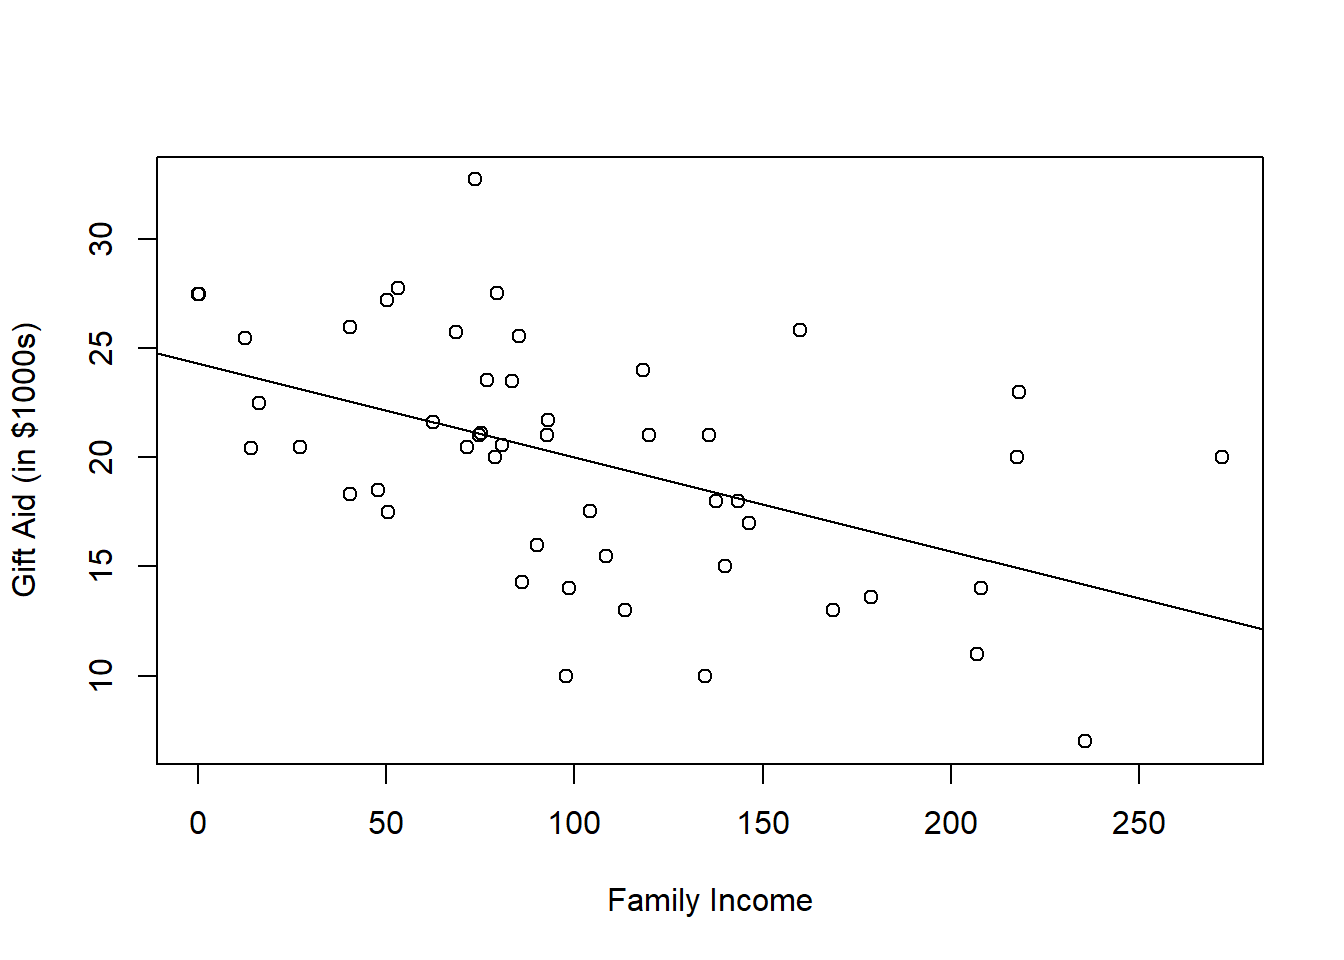
\includegraphics{bookdown-demo_files/figure-latex/elmhurst-1.pdf}
\caption{\label{fig:elmhurst}Scatterplot of Gift Aid Against Family Income}
\end{figure}

In Figure \ref{fig:elmhurst}, we see that the data points are evenly scattered around the fitted line. We also see the vertical variation of the data points is fairly constant. So assumptions that the errors have 0 mean and constant variance appear to be met.

\hypertarget{practice-question}{%
\subsubsection{Practice question}\label{practice-question}}

The data are about the prices of used cars. We are regressing the sale price of the car against the age of the car. The corresponding scatterplot is shown in Figure \ref{fig:mazda}. Based on Figure \ref{fig:mazda}, which of assumptions 1 or 2 (or both, or neither), is met? We will go over this in the tutorial.

\begin{figure}
\centering
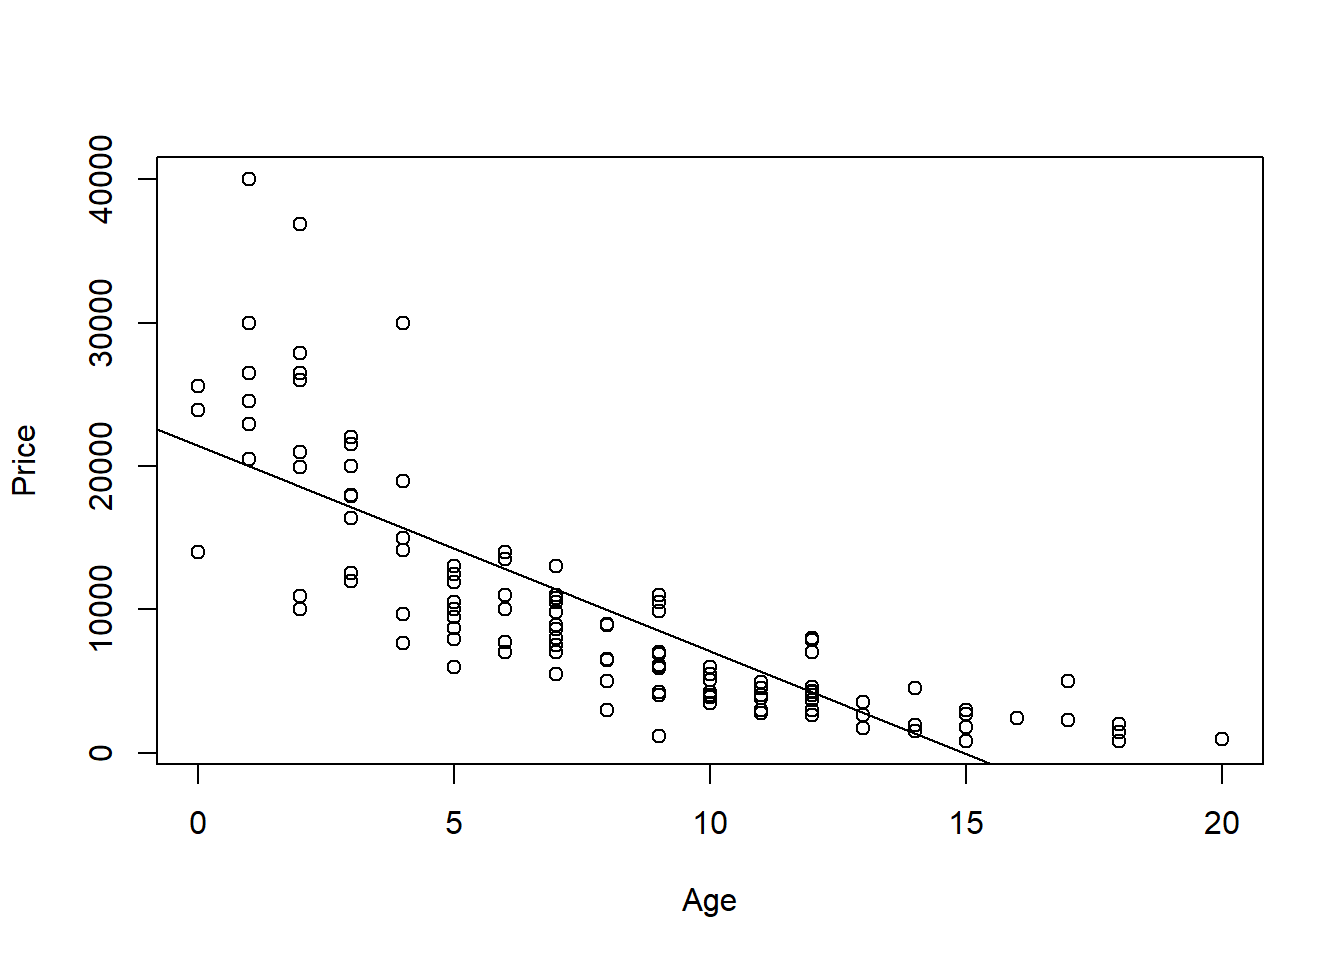
\includegraphics{bookdown-demo_files/figure-latex/mazda-1.pdf}
\caption{\label{fig:mazda}Scatterplot of Sale Price Against Age}
\end{figure}

\hypertarget{residual-plot}{%
\subsection{Residual plot}\label{residual-plot}}

While using the scatterplot is an intuitive way of assessing regression assumptions, it has a limitation. It cannot be used if we have multiple predictors in our regression, which we will encounter (and happens more often than just having one predictor). Another visualization that we can use to assess assumptions 1 and 2 is a \textbf{residual plot}. This is a scatterplot of residuals, \(e\), against fitted values, \(\hat{y}\). We want to observe the following in a residual plot.

\begin{itemize}
\tightlist
\item
  Residuals should be \textbf{evenly scattered} across the horizontal axis (assumption 1).
\item
  The residuals should have \textbf{similar vertical variation} across the plot (assumption 2).
\item
  Some writers combine these two points into the following statement: the residuals should fall in a \textbf{horizontal band around 0} with no apparent pattern (assumption 1, 2).
\end{itemize}

The residual plots in Figure \ref{fig:resplots} are based on simulated data from Figures \ref{fig:ass1}(a), \ref{fig:ass1}(b), and \ref{fig:ass2}(b).

\begin{figure}
\centering
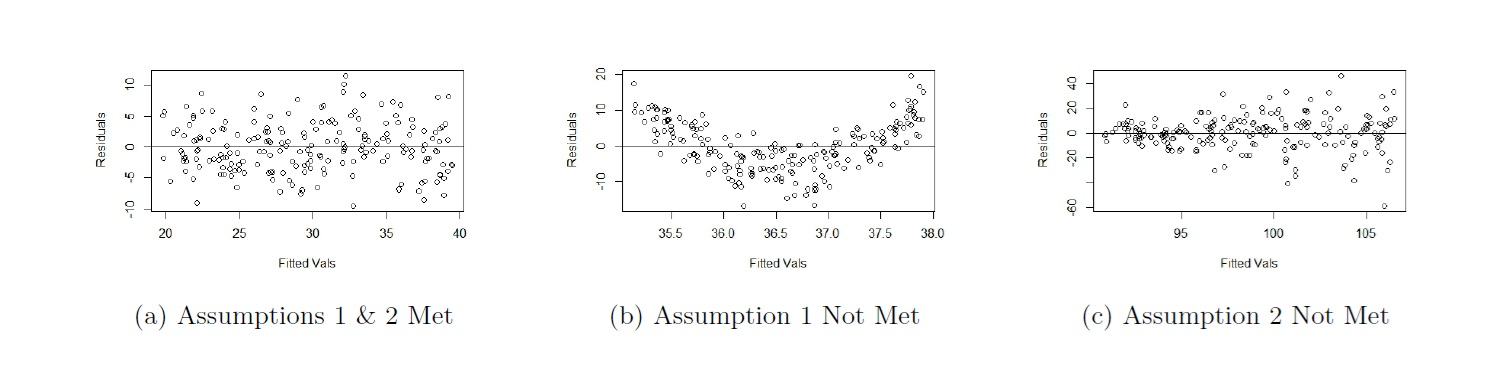
\includegraphics{images/resplots.jpg}
\caption{\label{fig:resplots}Residual Plots from Fig 1(a), 1(b), 2(b) Respectively}
\end{figure}

We make the following observations:

\begin{itemize}
\tightlist
\item
  From Figure \ref{fig:resplots}(a), we see that the residuals are evenly scattered across the horizontal axis, and their vertical variation is fairly constant across the plot. So both assumptions are met.
\item
  From Figure \ref{fig:resplots}(b), we see that the residuals are \textbf{not} evenly scattered across the horizontal axis, although their vertical variation is fairly constant across the plot. So only assumption 1 is not met.
\item
  From Figure \ref{fig:resplots}(c), we see that the residuals are evenly scattered across the horizontal axis, but their vertical variation is \textbf{not constant} across the plot. In fact, the vertical variation is increasing as we move from left to right. So only assumption 2 is not met.
\end{itemize}

If you compare the conclusions from the residuals plots and scatterplots, they are the same. In SLR, the takeaways should be consistent.

\emph{Please see the associated video for more explanation on how to use Figure \ref{fig:resplots} to assess assumptions 1 and 2.}

\hypertarget{practice-questions-2}{%
\subsubsection{Practice questions}\label{practice-questions-2}}

\begin{enumerate}
\def\labelenumi{\arabic{enumi}.}
\item
  The residual plot in Figure \ref{fig:practice}(a) comes from regressing gift aid against family income for the \texttt{elmhurst} dataset. Based on this residual plot, which assumptions are met?
\item
  The residual plot in Figure \ref{fig:practice}(b) comes from regressing price of cars against age for the used cars dataset. Based on this residual plot, which assumptions are met?
\end{enumerate}

\emph{Please see the associated video as I go over these practice questions.}

\begin{figure}
\centering
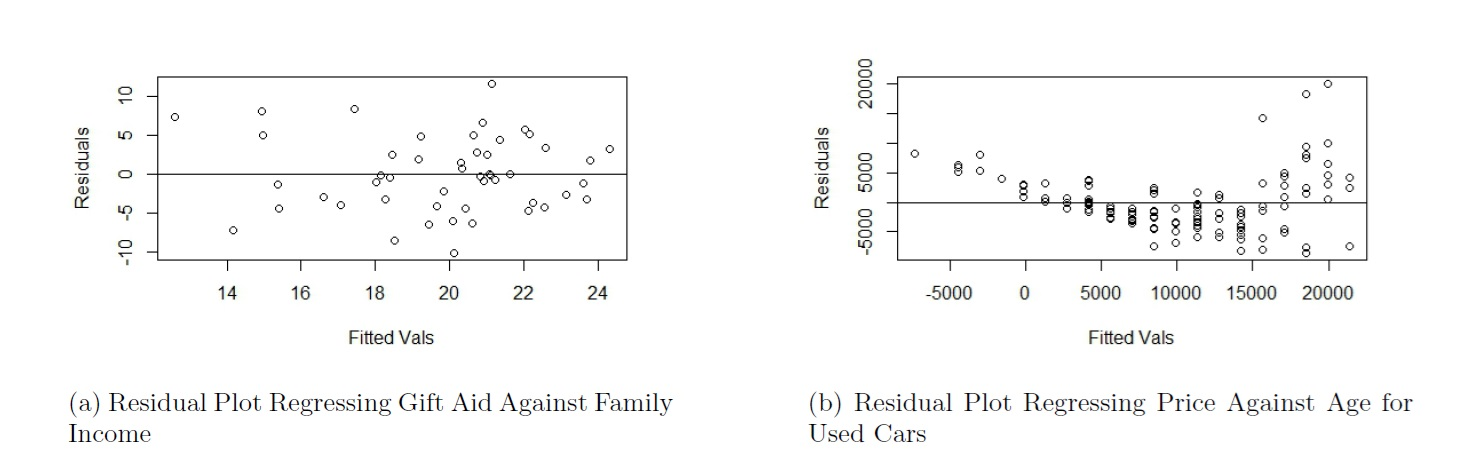
\includegraphics{images/practice.jpg}
\caption{\label{fig:practice}Residual Plots for Practice Questions}
\end{figure}

\hypertarget{acf-plot}{%
\subsection{ACF plot}\label{acf-plot}}

Assumption 3 states that the errors are \textbf{independent}. This assumption implies that the values of the response variable are independent from each other. This assumption is typically assessed via knowing the nature of the data.

\begin{itemize}
\item
  If the observations were obtained from a random sample, it is likely that the observations will be independent from each other. This is the very nature of a random sample and why random samples are preferred over convenience samples.
\item
  If the data has some inherent sequence, it is likely the observations will not be independent, and are dependent. For example, if I record the value of a stock at the end of each day, the value at day 2 is likely to be related to its value at day 1. So the values of stock prices at the end of each day are not independent.
\end{itemize}

An autocorrelation function (ACF) plot of the residuals may be a used to help assess if the assumption that the errors are independent is met. However, the plot is not a substitute for using your understanding about the nature of the data and should only be used as a confirmation.

The ACF plot measures the correlation between a vector of observations and the lagged versions of the observations. If the observations are uncorrelated, the correlations between the vector of observations and lagged versions of these observations are theoretically 0. We may create an ACF plot for the residuals from our regression.

The ACF plot in Figure \ref{fig:ass3}(a) and is based on simulated data that were independently generated.

\begin{figure}
\centering
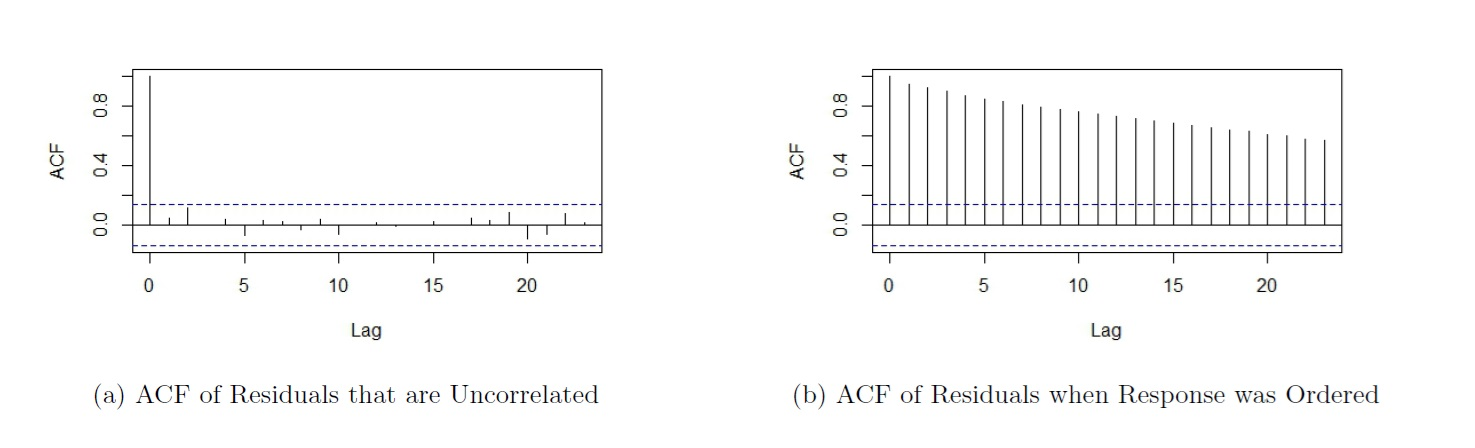
\includegraphics{images/ass3.jpg}
\caption{\label{fig:ass3}Assumption 3}
\end{figure}

A few notes about the ACF plot:

\begin{itemize}
\tightlist
\item
  The ACF at lag 0 is always 1. The correlation of any vector with itself is always 1.
\item
  The dashed horizontal lines represent critical values. An ACF at any lag beyond the critical value indicates an ACF that is significant. We have evidence of correlation (and hence dependence) in our residuals.
\item
  If the observed values for the response variable are independent, then we would expect the ACFs at lags greater than 0 to be insignificant. Do note that because we are conducting multiple hypothesis tests, do not be too alarmed if the ACFs are slightly beyond the critical values at an isolated lag or 2.
\end{itemize}

Based on Figure \ref{fig:ass3}(a), we see that the ACFs at all lags greater than 0 are insignificant. We do not have evidence the residuals are correlated with each other, so we do not have evidence that assumption 3 is not met.

Sometimes, the dataframe can be sorted in some manner (e.g.~increasing order for response variable), and if so, we would actually expect to see significant correlations in the ACF plot. The ACF plot in Figure \ref{fig:ass3}(b) is such an example. The residuals are from the same simulated dataset, only with the data sorted by the response variable. If we had just looked at the ACF plot in Figure \ref{fig:ass3}(b) without understanding the data were simulated independently and then sorted, we would have erroneously concluded that the residuals are not independent and the regression assumption is not met.

\hypertarget{qq-plot}{%
\subsection{QQ plot}\label{qq-plot}}

A normal probability plot (also called a QQ plot) is used to assess if the distribution of a variable is normal. It typically plots the residuals against their theoretical residual if they followed a normal distribution. A QQ line is typically overlaid. If the plots fall closely to the QQ line, we have evidence that the observations follow a normal distribution. Figure \ref{fig:qq} shows a QQ plot that comes from a normally distributed variable.

\begin{figure}
\centering
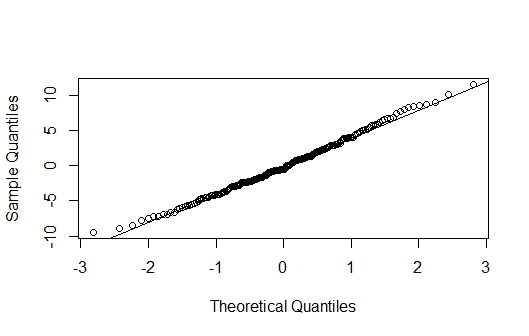
\includegraphics{images/qqplot.jpeg}
\caption{\label{fig:qq}QQ Plot}
\end{figure}

\hypertarget{remedial-measures}{%
\subsection{Remedial measures}\label{remedial-measures}}

We now know how to assess if specific regression assumptions are not met. The remedial measures involve transforming either the predictor variable and / or the response variable. These transformations are chosen to handle violations to assumptions 1 and / or 2 respectively. The general strategy on selecting which variable to transform:

\begin{itemize}
\tightlist
\item
  Transforming the response variable, \(y\), affects both assumptions 1 and 2.

  \begin{itemize}
  \tightlist
  \item
    Visually, we can think of transforming \(y\) in terms of stretching or squeezing the scatterplot of \(y\) against \(x\) vertically. Thus, transforming \(y\) affects the shape of the relationship and the vertical spread of the data points.
  \item
    However, the \textbf{choice on how we transform \(y\) is based on handling assumption 2.}
  \end{itemize}
\item
  Transforming the predictor variable, \(x\) affects assumption 1 and does not theoretically affect assumption 2.

  \begin{itemize}
  \tightlist
  \item
    Visually, we can think of transforming \(x\) in terms of stretching or squeezing the scatterplot of \(y\) against \(x\) horizontally. Thus, transforming \(x\) affects the shape of the relationship but not the vertical spread of the data points.
  \item
    Therefore, \textbf{transforming \(x\) is based on handling assumption 1.}
  \end{itemize}
\item
  If assumption 2 is not met, we transform \(y\) to stabilize the variance and make it constant.
\item
  If assumption 1 is not met, we transform \(x\) to find the appropriate shape to relate the variables.
\item
  If both assumptions are not met, we transform \(y\) first to stabilize the variance. Once assumption 2 is solved, check if assumption 1 is not met. If not met, transform \(x\).
\end{itemize}

Assumption 1 deals with whether the way we have expressed how \(y\) and \(x\) are related, through \(f(x)\), is appropriate. Assumption 2 deals with the vertical variation of the data points in the scatterplot.

\hypertarget{remedial-measures-variance-stabilizing-transformations}{%
\section{Remedial Measures: Variance Stabilizing Transformations}\label{remedial-measures-variance-stabilizing-transformations}}

We transform the response variable to stabilize the variance (assumption 2). There are a couple of ways to decide the appropriate transformation:

\begin{enumerate}
\def\labelenumi{\arabic{enumi}.}
\tightlist
\item
  Pattern seen in residual plot can guide choice in how to transform the response variable.
\item
  Box-Cox plot.
\end{enumerate}

\hypertarget{use-pattern-in-residual-plot}{%
\subsection{Use Pattern in Residual Plot}\label{use-pattern-in-residual-plot}}

We can stabilize the variance of the errors based on the residual plot, if we see either of the following scenarios:

\begin{itemize}
\tightlist
\item
  vertical variation of residuals \textbf{increasing} as fitted response increases, or as we move from left to right, as in Figure \ref{fig:variance}(a), or
\item
  vertical variation of residuals \textbf{decreasing} as fitted response increases, or as we move from left to right, as in Figure \ref{fig:variance}(b).
\end{itemize}

\begin{figure}
\centering
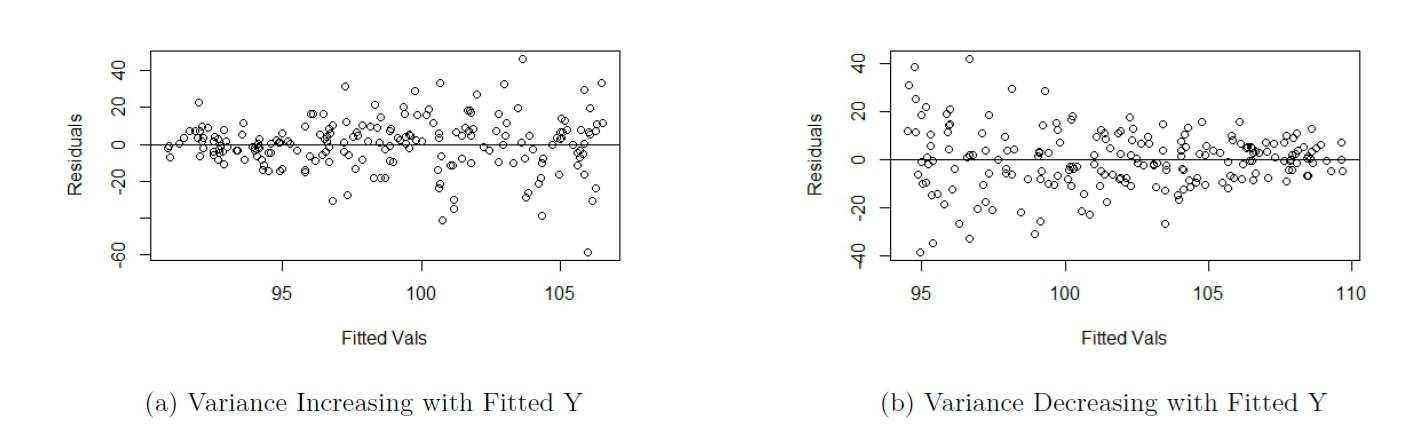
\includegraphics{images/variance.jpg}
\caption{\label{fig:variance}Non Constant Variance in Residual Plot}
\end{figure}

Note that increasing variance as fitted response increases is much more common with real data. Generally, larger values of a variable are associated with larger spread.

We transform \(y\) using \(y^{*} = y^{\lambda}\), with \(\lambda\) chosen based on whether the variance of the residuals is increasing or decreasing with fitted response:

\begin{itemize}
\tightlist
\item
  For Figure \ref{fig:variance}(a), choose \(\lambda < 1\).

  \begin{itemize}
  \tightlist
  \item
    If \(\lambda = 0\), it means we use a logarithmic transformation with base e, i.e.~\(y^* = \log(y)\).
  \item
    Note that a logarithm with no base means a natural log, or ln.
  \end{itemize}
\item
  For Figure \ref{fig:variance}(b), choose \(\lambda > 1\).
\end{itemize}

So based on the residual plot, we have a range of values for \(\lambda\).

\hypertarget{box-cox-plot}{%
\subsection{Box-Cox Plot}\label{box-cox-plot}}

We can use a Box-Cox plot to help us narrow the range of \(\lambda\) to use. It is a plot of the log-likelihood function against \(\lambda\), and we choose \(\lambda\) that maximizes this log-likelihood function. For example, Figure \ref{fig:bcplot} shows the Box Cox plot generated for the regression associated with the residual plot in Figure \ref{fig:variance}(b).

\begin{figure}
\centering
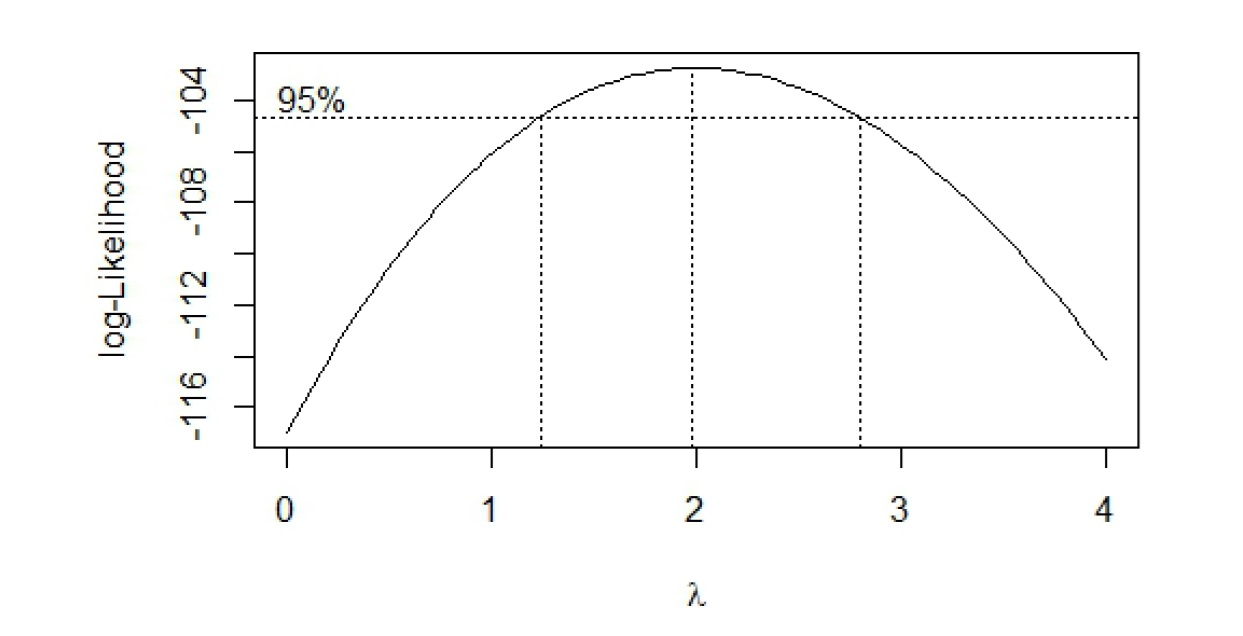
\includegraphics{images/bcplot.jpg}
\caption{\label{fig:bcplot}Box-Cox Plot based on Figure 9(b)}
\end{figure}

Notice an approximate 95\% CI is provided for \(\lambda\). A few comments on how to use the Box-Cox plot:

\begin{itemize}
\tightlist
\item
  Three vertical dashed lines are displayed: the middle line corresponds to the optimal value of \(\lambda\); the other two lines are the lower and upper bounds of a 95\% CI for \(\lambda\).
\item
  We choose \(\lambda\) within the CI (or even close to it) that is easy to understand. We do not have to choose the optimal value, especially if its value is difficult to interpret. In this example, I will choose \(\lambda = 2\), so a square transformation for \(y\). Transform response with \(y^* = y^2\). Regress \(y^*\) against \(x\).
\item
  If 1 lies in the CI, \textbf{no transformation} on \(y\) may be needed.
\item
  If a transformation is needed, a \textbf{log transformation} is preferred, since we can still interpret the estimated coefficients. It is difficult to interpret with any other type of transformation.
\item
  View the Box-Cox procedure as a guide for selecting a transformation, rather than being definitive.
\item
  Need to recheck the residuals after every transformation to assess if the transformation worked.
\end{itemize}

\hypertarget{interpretation-with-log-transformed-response}{%
\subsection{Interpretation with Log Transformed Response}\label{interpretation-with-log-transformed-response}}

A log transformation on the response is preferred over any other transformation, as we can still interpret regression coefficients. A couple of ways to interpret the estimated slope \(\hat{\beta}_1\):

\begin{itemize}
\tightlist
\item
  The predicted response variable is \textbf{multiplied by a factor} of \(\exp(\hat{\beta_1})\) for a one-unit increase in the predictor.
\item
  We can also subtract 1 from \(\exp(\hat{\beta_1})\) to express the change as a percentage.

  \begin{itemize}
  \tightlist
  \item
    If \(\hat{\beta}_1\) is positive, we have a percent \textbf{increase}. The predicted response variable increases by \((\exp(\hat{\beta_1}) - 1) \times 100\) percent for a one-unit increase in the predictor.
  \item
    If \(\hat{\beta}_1\) is negative, we have a percent \textbf{decrease}. The predicted response variable decreases by \((1 - \exp(\hat{\beta_1})) \times 100\) percent for a one-unit increase in the predictor.
  \end{itemize}
\end{itemize}

\emph{Please see the associated video as I go over the math explaining how we interpret regression coefficients when the response variable is log transformed.}

\hypertarget{remedial-measures-linearization-transformations}{%
\section{Remedial Measures: Linearization Transformations}\label{remedial-measures-linearization-transformations}}

We first ensure the variance has been stabilized and assumption 2 is met. If \(f(x)\) does not accurately capture the relationship between the variables, we transform the predictor variable to meet assumption 1. Some writers call this a linearization transformation, as we seek to make the transformed version of the predictor variable, \(x^*\), to be approximately linear with the response variable (or transformed \(y\)), i.e.~\(y = \beta_0 + \beta_1 x^* + \epsilon\). We do not consider transforming the response variable to deal with assumption 1, as transforming the response variable is likely to reintroduce violation of assumption 2.

The general strategy on how to transform the predictor is via a scatterplot of \(y\) (or \(y^*\)) against \(x\). We use the pattern seen in the plot to decide how to transform the predictor. Some examples are shown in Figure \ref{fig:xstar} below.

\begin{figure}
\centering
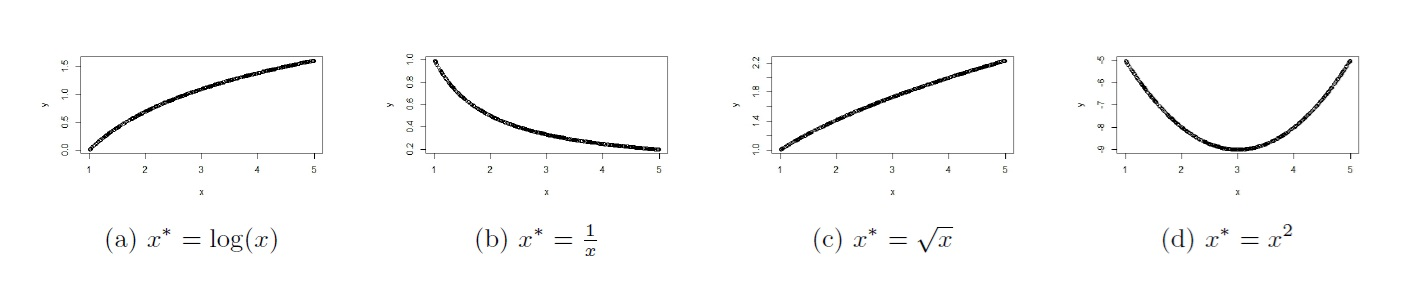
\includegraphics{images/xstar.jpg}
\caption{\label{fig:xstar}Transformations for x}
\end{figure}

\hypertarget{hierarchical-principle}{%
\subsection{Hierarchical Principle}\label{hierarchical-principle}}

One thing to be aware of is the \textbf{hierarchical principle}: if the relationship between the response and predictor is of a higher order polynomial (e.g.~quadratic, cubic), the hierarchical principle states that the lower order terms should remain in the model. For example, if the relationship is of order \(h\), fit \(y = \beta_0 + \beta_1 x + \beta_2 x^2 + \cdots + \beta_h x^h + \epsilon\) via a multiple linear regression framework. We will see how to do this in the next module.

\hypertarget{interpretation-with-log-transformed-predictor}{%
\subsection{Interpretation with Log Transformed Predictor}\label{interpretation-with-log-transformed-predictor}}

A log transformation on the predictor is preferred over any other transformation, as we can still interpret the regression coefficient, \(\hat{\beta}_1\), in a couple of ways:

\begin{itemize}
\tightlist
\item
  For an \(a\%\) increase in the predictor, the predicted response \textbf{increases by \(\hat{\beta}_1 \log(1+ \frac{a}{100})\).}
\item
  \(\log(1 + \frac{1}{100}) \approx \frac{1}{100}\) (Taylor series). So an alternative interpretation is: for a 1\% increase in the predictor, the predicted response increases by approximately \(\frac{\hat{\beta}_1}{100}\).
\end{itemize}

\emph{Please see the associated video as I go over the math explaining how we interpret regression coefficients when the predictor variable is log transformed.}

\hypertarget{interpretation-with-log-transformed-response-and-predictor}{%
\subsection{Interpretation with Log Transformed Response and Predictor}\label{interpretation-with-log-transformed-response-and-predictor}}

If both response and predictor variables are log transformed, the regression coefficient, \(\hat{\beta}_1\), can be interpreted in a couple of ways:

\begin{itemize}
\item
  For an \(a\%\) increase in the predictor, the predicted response is \textbf{multiplied by \((1 + \frac{a}{100})^{\hat{\beta}_1}\).}
\item
  \((1 + \frac{1}{100})^{\hat{\beta}_1} \approx 1 + \frac{\hat{\beta}_1}{100}\) (Taylor series). So an alternative interpretation is: for a 1\% increase in the predictor, the predicted response \textbf{increases by approximately \(\hat{\beta}_1\) percent.} Note that this approximation works better when \({\hat{\beta}_1}\) is small in magnitude.
\end{itemize}

\emph{Please see the associated video as I go over the math explaining how we interpret regression coefficients when the both response and predictor variables are log transformed.}

\hypertarget{some-general-comments-about-assessing-assumptions-and-transformations}{%
\subsection{Some General Comments about Assessing Assumptions and Transformations}\label{some-general-comments-about-assessing-assumptions-and-transformations}}

\begin{itemize}
\item
  When assessing the assumptions with a residual plot, we are assessing if the assumptions are reasonably / approximately met.
\item
  With real data, assumptions are rarely met 100\%.
\item
  If unsure, proceed with model building, and test how model performs on new data. If poor performance, go back to residual plot to assess what transformation will be appropriate.
\item
  Assess the plots to decide which variables need to be transformed, and how. The choice of transformation should be guided by what you see in the plots, and not by trial and error.
\item
  A residual plot should always be produced after each transformation. A Box Cox plot could also be produced. The plots should be assessed if the transformation helped in the way you intended.
\item
  Solve assumption 2 first, then assumption 1.
\end{itemize}

\hypertarget{r-tutorial-2}{%
\section{R Tutorial}\label{r-tutorial-2}}

\hypertarget{example-1}{%
\subsection{Example 1}\label{example-1}}

The linear regression model involves several assumptions. Among them are:

\begin{enumerate}
\def\labelenumi{\arabic{enumi}.}
\tightlist
\item
  The errors, for each fixed value of \(x\), have mean 0. This implies that the relationship as specified in the regression equation is appropriate.
\item
  The errors, for each fixed value of \(x\), have constant variance. That is, the variation in the errors is theoretically the same regardless of the value of \(x\) (or \(\hat{y}\)).
\item
  The errors are independent.
\item
  The errors, for each fixed value of \(x\), follow a normal distribution.
\end{enumerate}

To assess assumptions 1 and 2, we can examine scatterplots of:

\begin{itemize}
\tightlist
\item
  \(y\) versus \(x\).
\item
  residuals versus fitted values, \(\hat{y}\).
\end{itemize}

Assumption 3 is assessed based on knowledge of the data. An autocorrelation (ACF) plot of the residuals may also be used.

Assumption 4 is assessed with a normal probability plot, and is considered the least crucial of the assumptions.

We will see how to generate the relevant graphical displays to help us assess whether the assumptions are met, and if needed, carry out transformations on the variable(s) so the assumptions are met.

For this tutorial, we will go over a dataset involving prices of used cars (Mazdas). The two variables are the sales price of the used car, and the age of the car in years. Download the data file, \texttt{mazda.txt} and read the data:

\begin{Shaded}
\begin{Highlighting}[]
\NormalTok{Data}\OtherTok{\textless{}{-}}\FunctionTok{read.table}\NormalTok{(}\StringTok{"mazda.txt"}\NormalTok{, }\AttributeTok{header=}\ConstantTok{TRUE}\NormalTok{, }\AttributeTok{sep=}\StringTok{""}\NormalTok{)}
\end{Highlighting}
\end{Shaded}

\hypertarget{model-diagnostics-with-scatterplots}{%
\subsubsection*{Model Diagnostics with Scatterplots}\label{model-diagnostics-with-scatterplots}}
\addcontentsline{toc}{subsubsection}{Model Diagnostics with Scatterplots}

We can use a scatterplot of the response variable against the predictor to assess assumptions 1 and 2:

\begin{Shaded}
\begin{Highlighting}[]
\FunctionTok{library}\NormalTok{(tidyverse)}

\DocumentationTok{\#\#scatterplot, and overlay regression line}
\NormalTok{ggplot2}\SpecialCharTok{::}\FunctionTok{ggplot}\NormalTok{(Data, }\FunctionTok{aes}\NormalTok{(}\AttributeTok{x=}\NormalTok{Age,}\AttributeTok{y=}\NormalTok{Price))}\SpecialCharTok{+}
  \FunctionTok{geom\_point}\NormalTok{()}\SpecialCharTok{+}
  \FunctionTok{geom\_smooth}\NormalTok{(}\AttributeTok{method =} \StringTok{"lm"}\NormalTok{, }\AttributeTok{se=}\ConstantTok{FALSE}\NormalTok{)}\SpecialCharTok{+}
  \FunctionTok{labs}\NormalTok{(}\AttributeTok{x=}\StringTok{"Age"}\NormalTok{, }\AttributeTok{y=}\StringTok{"Sales Price"}\NormalTok{, }\AttributeTok{title=}\StringTok{"Scatterplot of Sales Price against Age"}\NormalTok{)}
\end{Highlighting}
\end{Shaded}

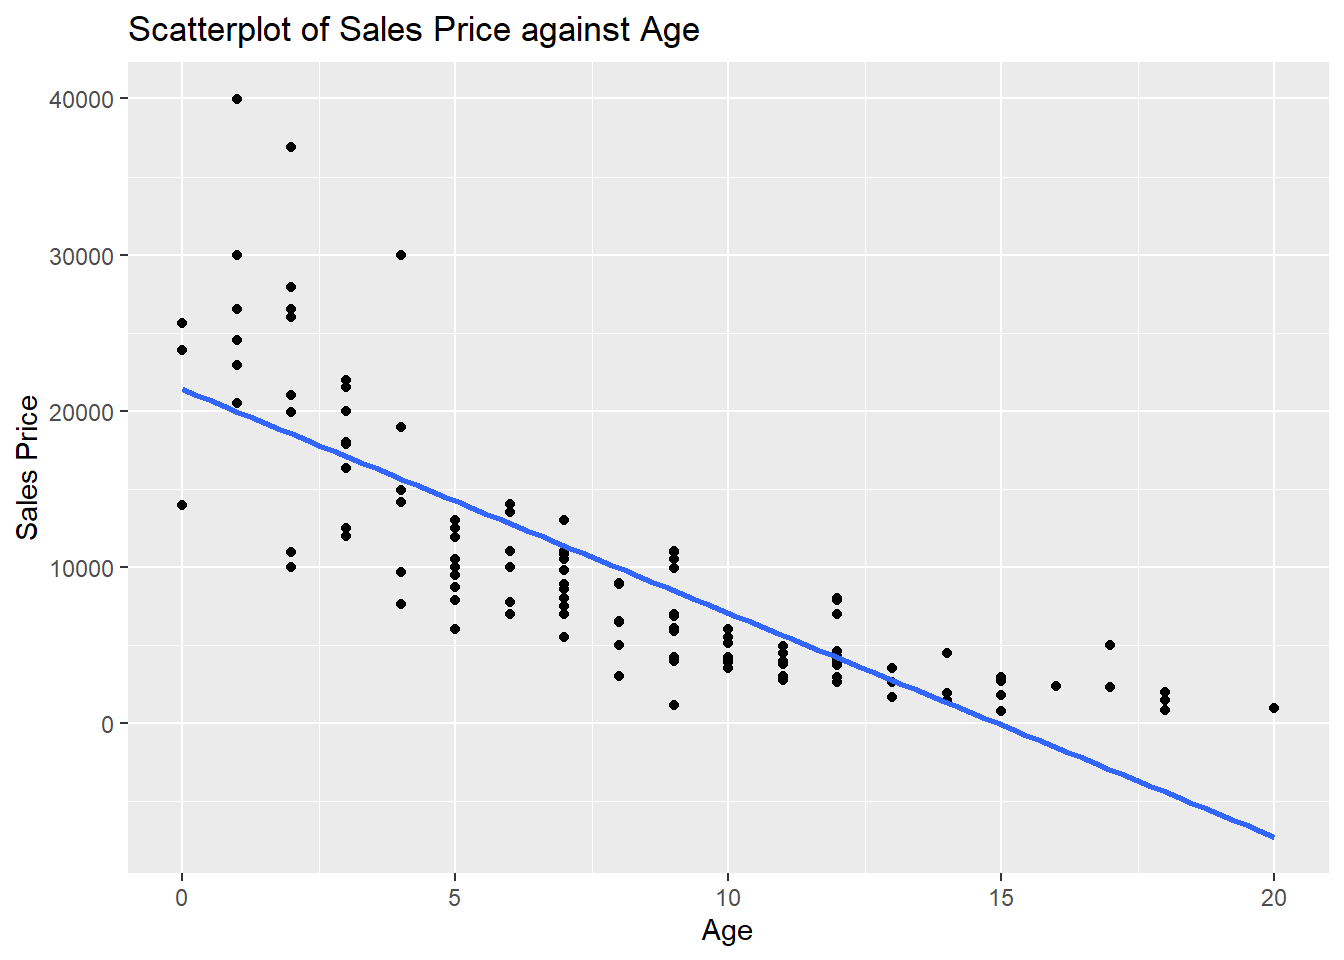
\includegraphics{bookdown-demo_files/figure-latex/unnamed-chunk-154-1.pdf}

To assess assumption 1, the data points should be evenly scattered on both sides of the regression line, as we move from left to right. We do not see this in the scatterplot, so assumption 1 is not met. When age is between 0 and 2, the data points are mostly above the line. When age is between 5 and 11, the data points are mostly below the line, and when age is greater than 13, the data points are above the line.

To assess assumption 2, the vertical spread of the data points should be constant as we move from left to right. The spread seems to be decreasing as we move from left to right (or in other words, the spread is increasing as the response increases), so assumption 2 is not met.

\hypertarget{model-diagnostics-with-residual-plots}{%
\subsubsection*{Model Diagnostics with Residual Plots}\label{model-diagnostics-with-residual-plots}}
\addcontentsline{toc}{subsubsection}{Model Diagnostics with Residual Plots}

Sometimes, a residual plot is easier to visualize than a scatterplot. We fit our SLR model using \texttt{lm()} as usual. Applying the \texttt{plot()} function to an object created with \texttt{lm()} actually produces a four diagnostic plots. To display the four diagnostic plots in a 2 by 2 array, we specify \texttt{par(mfrow\ =\ c(2,\ 2))} so the plotting window is split into a 2 by 2 array:

\begin{Shaded}
\begin{Highlighting}[]
\NormalTok{result}\OtherTok{\textless{}{-}}\FunctionTok{lm}\NormalTok{(Price}\SpecialCharTok{\textasciitilde{}}\NormalTok{Age, }\AttributeTok{data=}\NormalTok{Data)}
\FunctionTok{par}\NormalTok{(}\AttributeTok{mfrow =} \FunctionTok{c}\NormalTok{(}\DecValTok{2}\NormalTok{, }\DecValTok{2}\NormalTok{))}
\FunctionTok{plot}\NormalTok{(result)}
\end{Highlighting}
\end{Shaded}

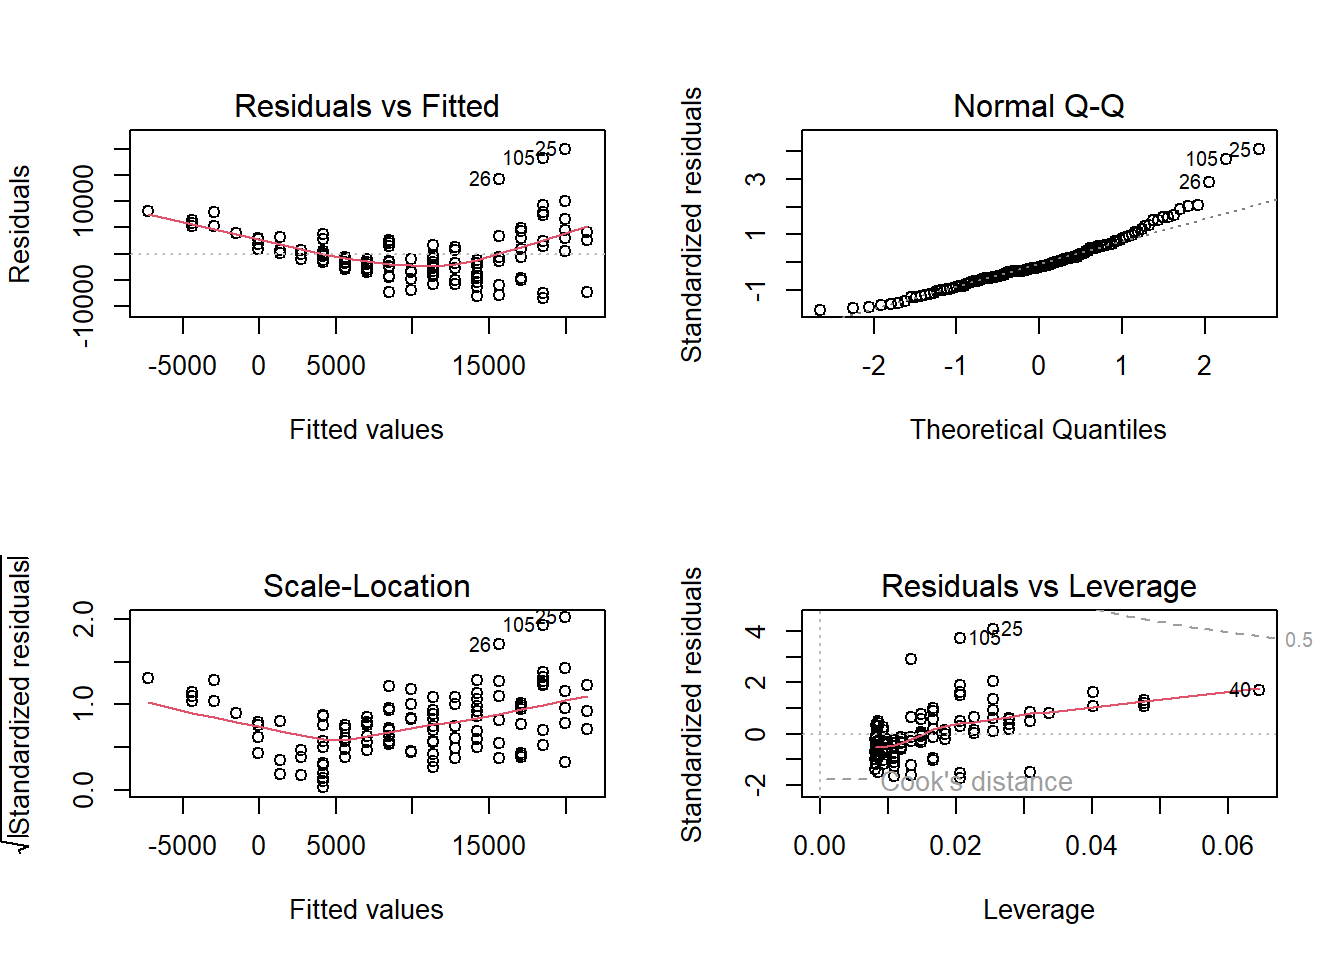
\includegraphics{bookdown-demo_files/figure-latex/unnamed-chunk-155-1.pdf}

\begin{itemize}
\item
  The first plot (top left) is the residual plot, with residuals on the y-axis and fitted values on the x-axis. The residual plot can be used to address assumptions 1 and 2. A red line is overlayed to represent the average value of the residuals for differing values along the x-axis. This line should be along the x-axis without any apparent curvature to indicate the form of our model is reasonable. This is not what we see, as we see a clear curved pattern. So assumption 1 is not met. For assumption 2, we want to see the vertical spread of the residuals to be fairly constant as we move from left to right. We do not see this in the residual plot; the vertical spread increases as we move from left to right, so assumption 2 is not met.
\item
  The second plot (top right) is the normal probability plot (also called a QQ plot), and addresses assumption 4. If the residuals are normal, the residuals should fall along the 45 degree line. The regression model is fairly robust to this assumption though; the normality assumption is the least crucial of the four.
\item
  The third plot (bottom left) is a plot of the square root of the absolute value of the standardized residuals against the fitted values (scale-location). This plot should be used to assess assumption 2, the constant variance assumption. A red line is overlayed to represent the average value on the vertical axis for differing values along the x-axis. If the variance is constant, the red line should be horizontal and the vertical spread of the plot should be constant. This plot should be used to assess assumption 2, if we have a small sample size. Otherwise, this plot should tell a similar story to the first plot (top left) when assessing assumption 2.
\item
  The last plot (bottom right) is a plot to identify influential outliers. Data points that lie in the contour lines with large Cook's distance are influential. None of our data points have Cook's distance greater than 0.5. As a general rule of thumb, observations with Cook's distance greater than 1 are flagged as influential. We will talk more about influential observations in a future module.
\end{itemize}

Now that we know that both assumptions 1 and 2 are not met. We need to transform the response variable first, to stabilize the variance.

Based on the residual plot, we see that the variance of the residuals increases as we move from left to right. So we know we need to transform the response variable using \(y^* = y^\lambda\) with \(\lambda < 1\). A log transform should be considered since we can still interpret regression coefficients.

\hypertarget{box-cox-transformation-on-y}{%
\subsubsection*{Box Cox Transformation on y}\label{box-cox-transformation-on-y}}
\addcontentsline{toc}{subsubsection}{Box Cox Transformation on y}

The Box Cox plot can be used to decide how to transform the response variable. The transformation takes the form \(y^* = y^{\lambda}\), with the value of \(\lambda\) to be chosen. If \(\lambda = 0\), we perform a \(\log\) transformation.

We will use the \texttt{boxcox()} function from the \texttt{MASS} package:

\begin{Shaded}
\begin{Highlighting}[]
\FunctionTok{library}\NormalTok{(MASS) }\DocumentationTok{\#\#to use boxcox function}
\NormalTok{MASS}\SpecialCharTok{::}\FunctionTok{boxcox}\NormalTok{(result)}
\end{Highlighting}
\end{Shaded}

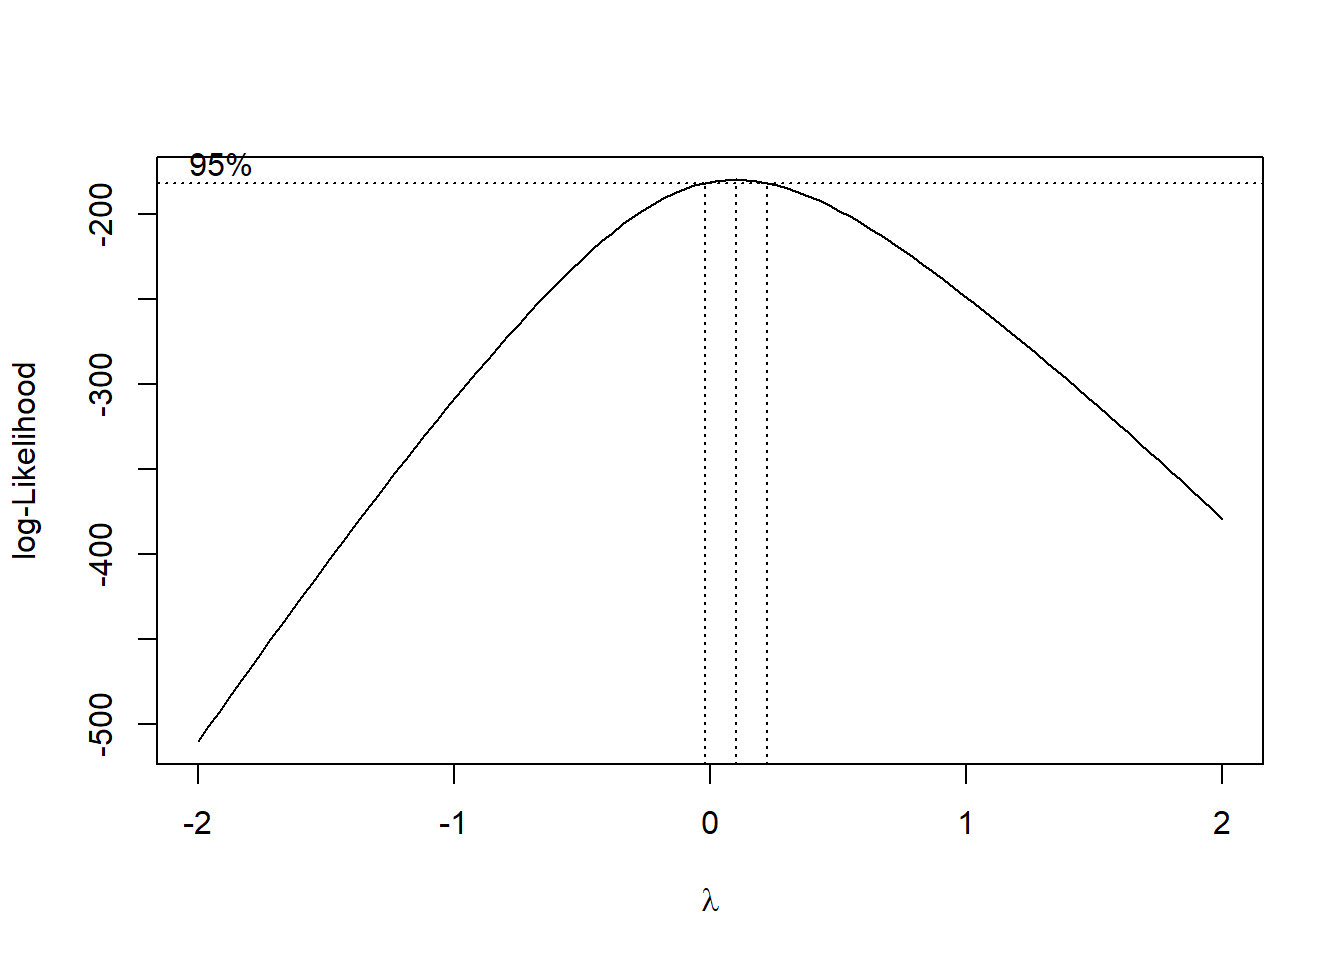
\includegraphics{bookdown-demo_files/figure-latex/unnamed-chunk-156-1.pdf}

We can ``zoom in'' on the plot to have a better idea about the value of \(\lambda\) we can use, by specifying the range of \texttt{lambda} inside the function:

\begin{Shaded}
\begin{Highlighting}[]
\DocumentationTok{\#\#adjust lambda for better visualization. Choose lambda between {-}0.5 and 0.5}
\NormalTok{MASS}\SpecialCharTok{::}\FunctionTok{boxcox}\NormalTok{(result, }\AttributeTok{lambda =} \FunctionTok{seq}\NormalTok{(}\SpecialCharTok{{-}}\FloatTok{0.5}\NormalTok{, }\FloatTok{0.5}\NormalTok{, }\DecValTok{1}\SpecialCharTok{/}\DecValTok{10}\NormalTok{)) }
\end{Highlighting}
\end{Shaded}

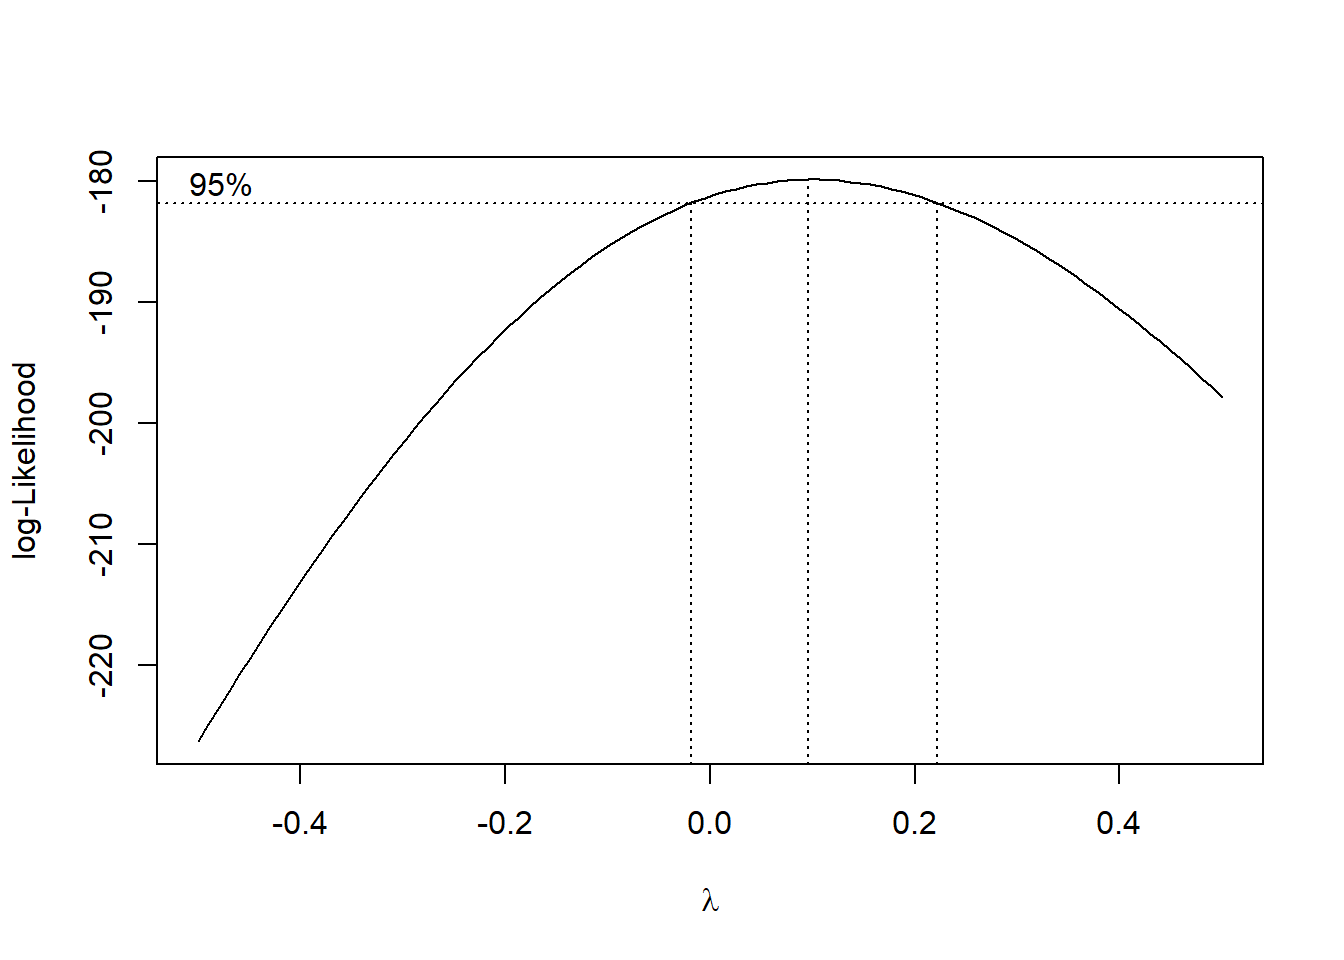
\includegraphics{bookdown-demo_files/figure-latex/unnamed-chunk-157-1.pdf}

We can choose any value of \(\lambda\) within the CI. A log transformation is preferred if possible, since we can still interpret coefficients. Since 0 lies in the CI, we choose \(\lambda = 0\), to log transform the response variable to get \(y^* = \log(y)\). We regress \(y^*\) against \(x\), and check the resulting residual plot:

\begin{Shaded}
\begin{Highlighting}[]
\DocumentationTok{\#\#transform y and then regress ystar on x}
\NormalTok{ystar}\OtherTok{\textless{}{-}}\FunctionTok{log}\NormalTok{(Data}\SpecialCharTok{$}\NormalTok{Price)}
\NormalTok{Data}\OtherTok{\textless{}{-}}\FunctionTok{data.frame}\NormalTok{(Data,ystar)}
\NormalTok{result.ystar}\OtherTok{\textless{}{-}}\FunctionTok{lm}\NormalTok{(ystar}\SpecialCharTok{\textasciitilde{}}\NormalTok{Age, }\AttributeTok{data=}\NormalTok{Data)}
\FunctionTok{par}\NormalTok{(}\AttributeTok{mfrow =} \FunctionTok{c}\NormalTok{(}\DecValTok{2}\NormalTok{, }\DecValTok{2}\NormalTok{))}
\FunctionTok{plot}\NormalTok{(result.ystar)}
\end{Highlighting}
\end{Shaded}

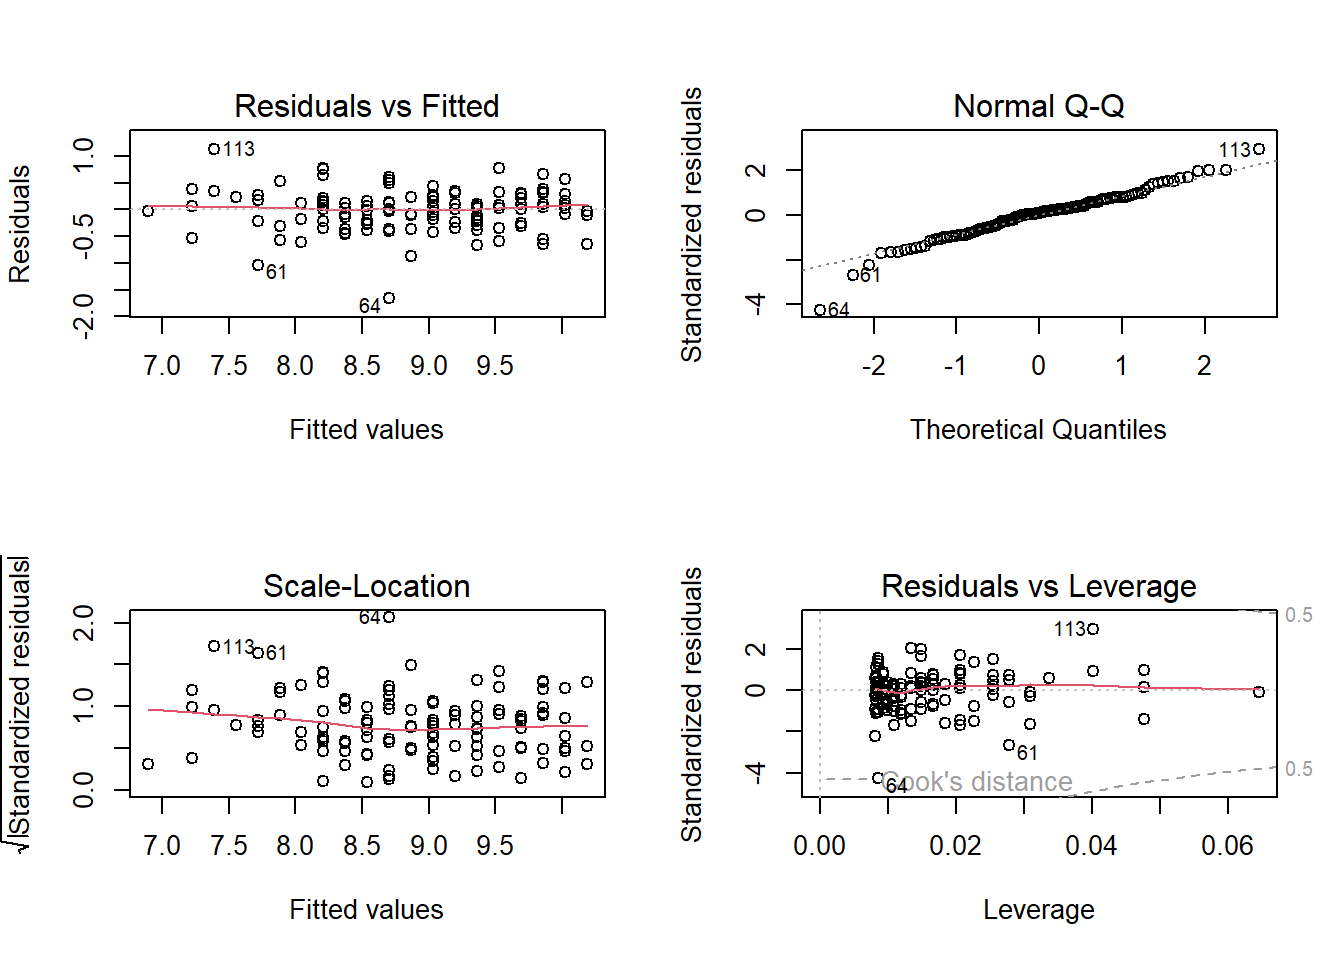
\includegraphics{bookdown-demo_files/figure-latex/unnamed-chunk-158-1.pdf}

We need to reassess assumptions 1 and 2 after the transformation.

\begin{itemize}
\item
  For assumption 2, we see that the vertical spread of the residuals in the residual plot (top left) is fairly constant, as we move from left to right. So assumption 2 is met. The log transformation worked.
\item
  We also notice that the residuals are now evenly scattered across the horizontal axis in the residual plot (top left). So assumption 1 is now met.
\end{itemize}

We do not need to perform any other transformations.

\hypertarget{interpreting-coefficients-with-log-transformed-response}{%
\subsubsection*{Interpreting Coefficients with Log Transformed Response}\label{interpreting-coefficients-with-log-transformed-response}}
\addcontentsline{toc}{subsubsection}{Interpreting Coefficients with Log Transformed Response}

So our regression equation is

\begin{Shaded}
\begin{Highlighting}[]
\NormalTok{result.ystar}
\end{Highlighting}
\end{Shaded}

\begin{verbatim}
## 
## Call:
## lm(formula = ystar ~ Age, data = Data)
## 
## Coefficients:
## (Intercept)          Age  
##     10.1878      -0.1647
\end{verbatim}

\(\hat{y^*} = 10.1878 - 0.1647x\), where \(y^* = \log(y)\). To interpret the slope:

\begin{itemize}
\tightlist
\item
  The price of used Mazdas is multiplied by \(\exp(-0.1647) = 0.8481481\) for each year older the car is.
\item
  The price of used Mazdas decreases by \((1 - 0.8481481) \times 100\) percent, or 15.18519 percent, for each year older the car is.
\end{itemize}

\hypertarget{acf-plot-of-residuals}{%
\subsubsection*{ACF Plot of Residuals}\label{acf-plot-of-residuals}}
\addcontentsline{toc}{subsubsection}{ACF Plot of Residuals}

We have yet to assess the assumption that the observed prices are independent from each other. Assuming that these prices are from different cars and not the same car measured repeatedly over time, there is no reason to think the prices are dependent on each other.

We an also produce an ACF plot to confirm our thought:

\begin{Shaded}
\begin{Highlighting}[]
\FunctionTok{acf}\NormalTok{(result.ystar}\SpecialCharTok{$}\NormalTok{residuals, }\AttributeTok{main=}\StringTok{"ACF Plot of Residuals with ystar"}\NormalTok{)}
\end{Highlighting}
\end{Shaded}

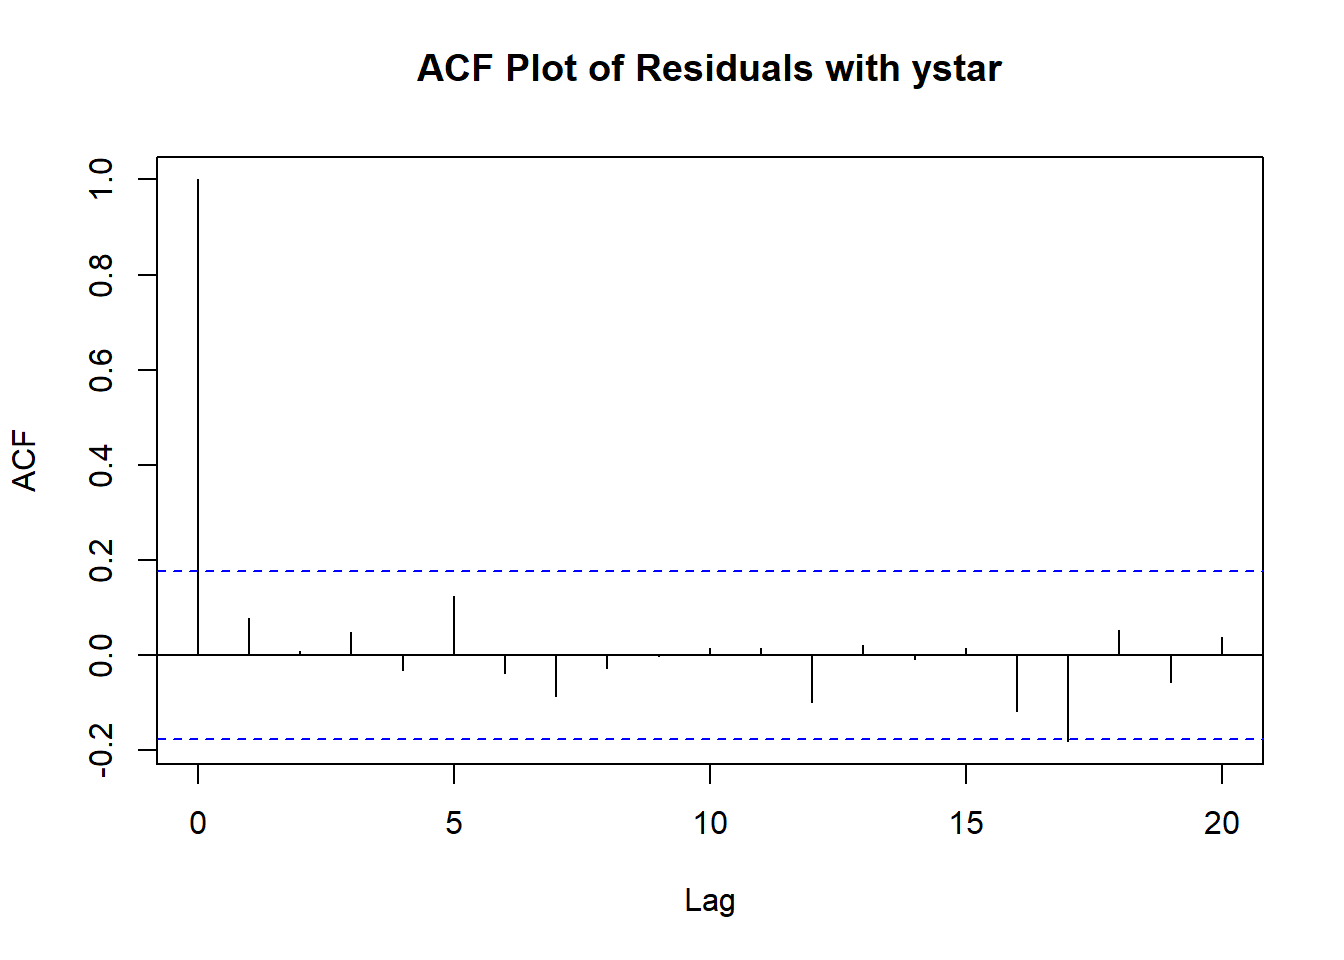
\includegraphics{bookdown-demo_files/figure-latex/unnamed-chunk-160-1.pdf}

None of the ACFs beyond lag 0 are significant, so we don't have evidence that the observations are dependent on each other.

\hypertarget{example-2}{%
\subsection{Example 2}\label{example-2}}

For this second example, we will go over an example for the \texttt{faraway} package. The dataframe is called \texttt{gala}. The data are about species diversity on the Galapagos Islands. There are 30 islands, and for each island, we have data on 7 variables. We will focus on the variable \texttt{Species}, which denotes the number of plant species found on the island, and \texttt{Area}, the area of the island in squared kilometers. We wish to see how the number of plant species of an island is related to the area of the island.

\begin{Shaded}
\begin{Highlighting}[]
\FunctionTok{library}\NormalTok{(faraway)}
\NormalTok{Data}\OtherTok{\textless{}{-}}\NormalTok{faraway}\SpecialCharTok{::}\NormalTok{gala}
\end{Highlighting}
\end{Shaded}

\hypertarget{model-diagnostics-with-scatterplots-1}{%
\subsubsection*{Model Diagnostics with Scatterplots}\label{model-diagnostics-with-scatterplots-1}}
\addcontentsline{toc}{subsubsection}{Model Diagnostics with Scatterplots}

We can use a scatterplot of the response variable against the predictor to assess assumptions 1 and 2.

\begin{Shaded}
\begin{Highlighting}[]
\FunctionTok{library}\NormalTok{(tidyverse)}

\DocumentationTok{\#\#scatterplot, and overlay regression line}
\NormalTok{ggplot2}\SpecialCharTok{::}\FunctionTok{ggplot}\NormalTok{(Data, }\FunctionTok{aes}\NormalTok{(}\AttributeTok{x=}\NormalTok{Area,}\AttributeTok{y=}\NormalTok{Species))}\SpecialCharTok{+}
  \FunctionTok{geom\_point}\NormalTok{()}\SpecialCharTok{+}
  \FunctionTok{geom\_smooth}\NormalTok{(}\AttributeTok{method =} \StringTok{"lm"}\NormalTok{, }\AttributeTok{se=}\ConstantTok{FALSE}\NormalTok{)}\SpecialCharTok{+}
  \FunctionTok{labs}\NormalTok{(}\AttributeTok{x=}\StringTok{"Area of Island (sq km)"}\NormalTok{, }\AttributeTok{y=}\StringTok{"\# of Plant Species"}\NormalTok{, }
       \AttributeTok{title=}\StringTok{"Scatterplot of Number of Plant Species against Area of Galapagos Island"}\NormalTok{)}
\end{Highlighting}
\end{Shaded}

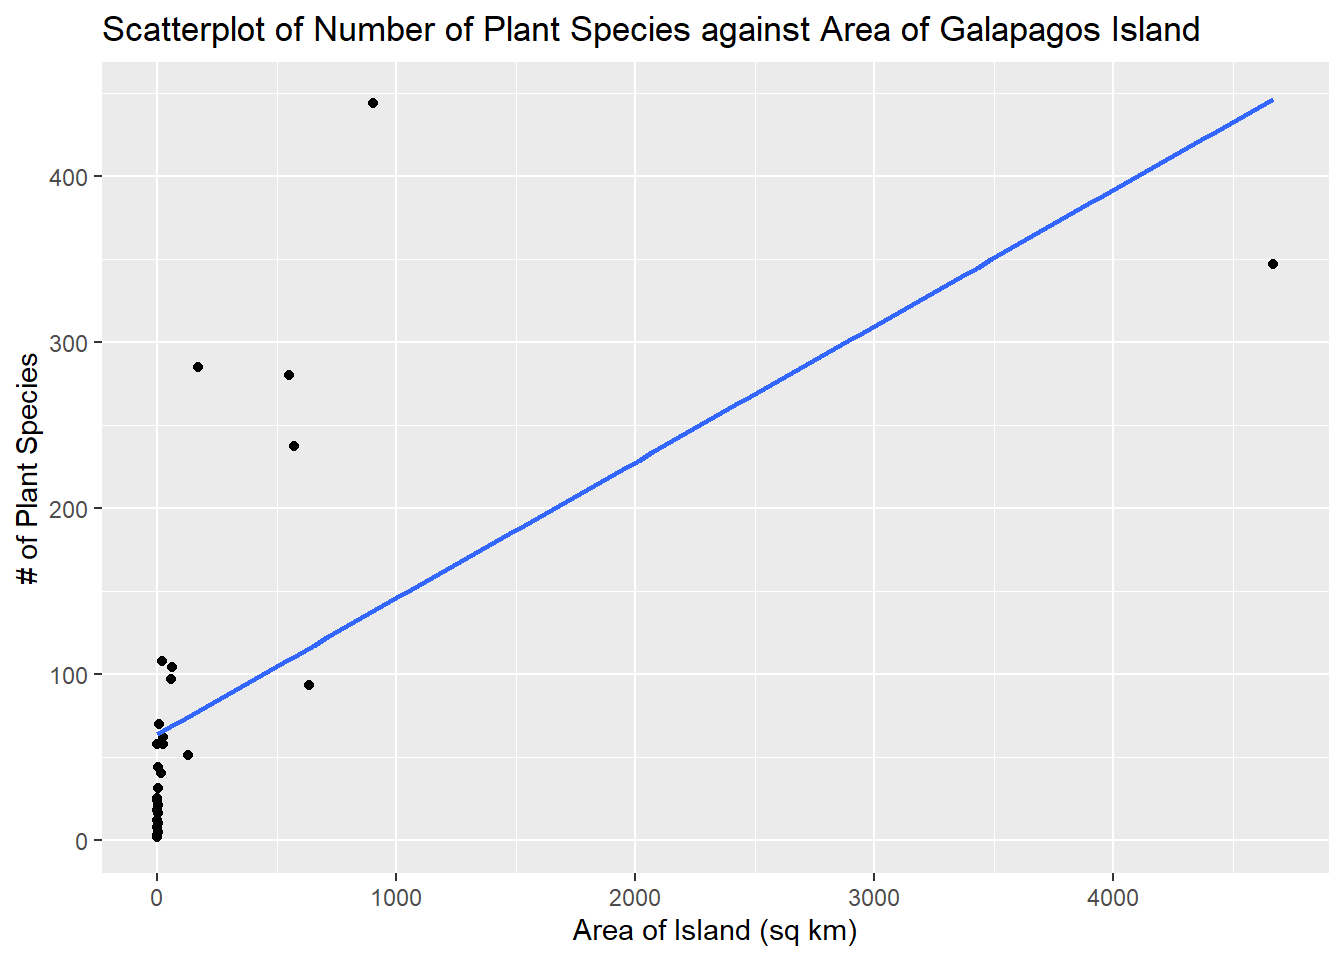
\includegraphics{bookdown-demo_files/figure-latex/unnamed-chunk-163-1.pdf}

To assess assumption 1, the data points should be evenly scattered on both sides of the regression line, as we move from left to right. This plot looks nonlinear.

To assess assumption 2, the vertical spread of the data points should be constant as we move from left to right. This can be a bit difficult to assess with this scatterplot, although observations with small areas are closer to the line, which suggests the assumption is not met.

\hypertarget{model-diagnostics-with-residual-plots-1}{%
\subsubsection*{Model Diagnostics with Residual Plots}\label{model-diagnostics-with-residual-plots-1}}
\addcontentsline{toc}{subsubsection}{Model Diagnostics with Residual Plots}

Fairly often, when assessing regression assumptions, a residual plot is easier to visualize than a scatterplot.

\begin{Shaded}
\begin{Highlighting}[]
\NormalTok{result}\OtherTok{\textless{}{-}}\FunctionTok{lm}\NormalTok{(Species}\SpecialCharTok{\textasciitilde{}}\NormalTok{Area, }\AttributeTok{data=}\NormalTok{Data)}
\FunctionTok{par}\NormalTok{(}\AttributeTok{mfrow =} \FunctionTok{c}\NormalTok{(}\DecValTok{2}\NormalTok{, }\DecValTok{2}\NormalTok{))}
\FunctionTok{plot}\NormalTok{(result)}
\end{Highlighting}
\end{Shaded}

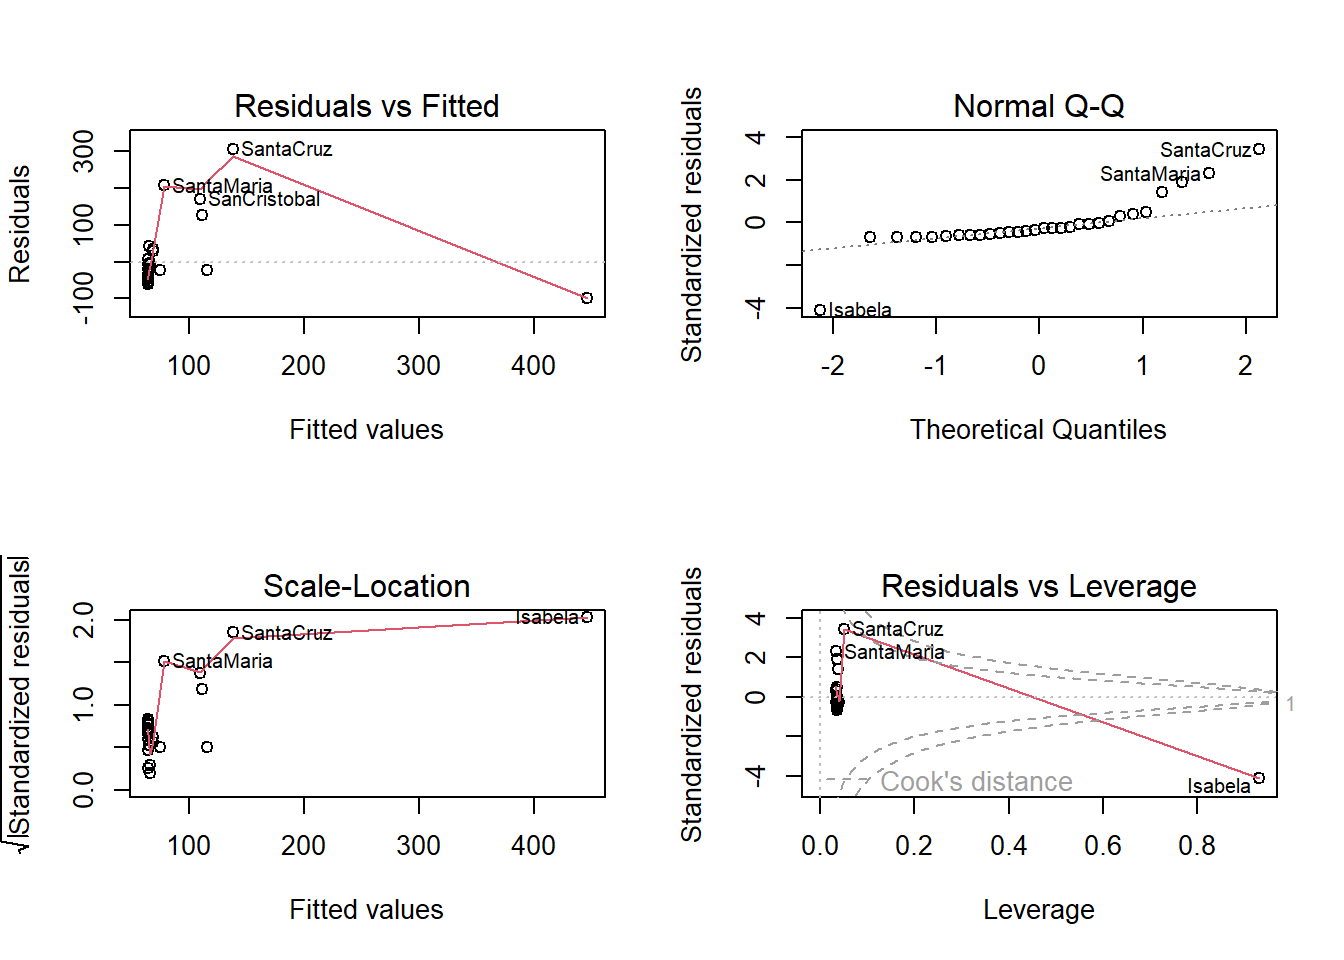
\includegraphics{bookdown-demo_files/figure-latex/unnamed-chunk-164-1.pdf}

\begin{itemize}
\item
  From the residual plot (top left), we see a curved pattern, so we have a nonlinear relationship. Assumption 1 is not met.
\item
  From the scale-location plot (bottom left), the vertical variance of the plots appear to be higher for islands with larger fitted valies, so assumption 2 is not met.
\end{itemize}

Now that we know that both assumptions 1 and 2 are not met. We need to transform the response variable first, to stabilize the variance.

\hypertarget{box-cox-transformation-on-y-1}{%
\subsubsection*{Box Cox Transformation on y}\label{box-cox-transformation-on-y-1}}
\addcontentsline{toc}{subsubsection}{Box Cox Transformation on y}

From the scale-location plot, we see the variance of the residuals is increasing, so we expect to transform the response variable with \(y^* = y^{\lambda}\) with \(\lambda < 1\). So see which specific value of \(\lambda\) to use, we can use the Box Cox plot:

\begin{Shaded}
\begin{Highlighting}[]
\FunctionTok{library}\NormalTok{(MASS)}
\NormalTok{MASS}\SpecialCharTok{::}\FunctionTok{boxcox}\NormalTok{(result)}
\end{Highlighting}
\end{Shaded}

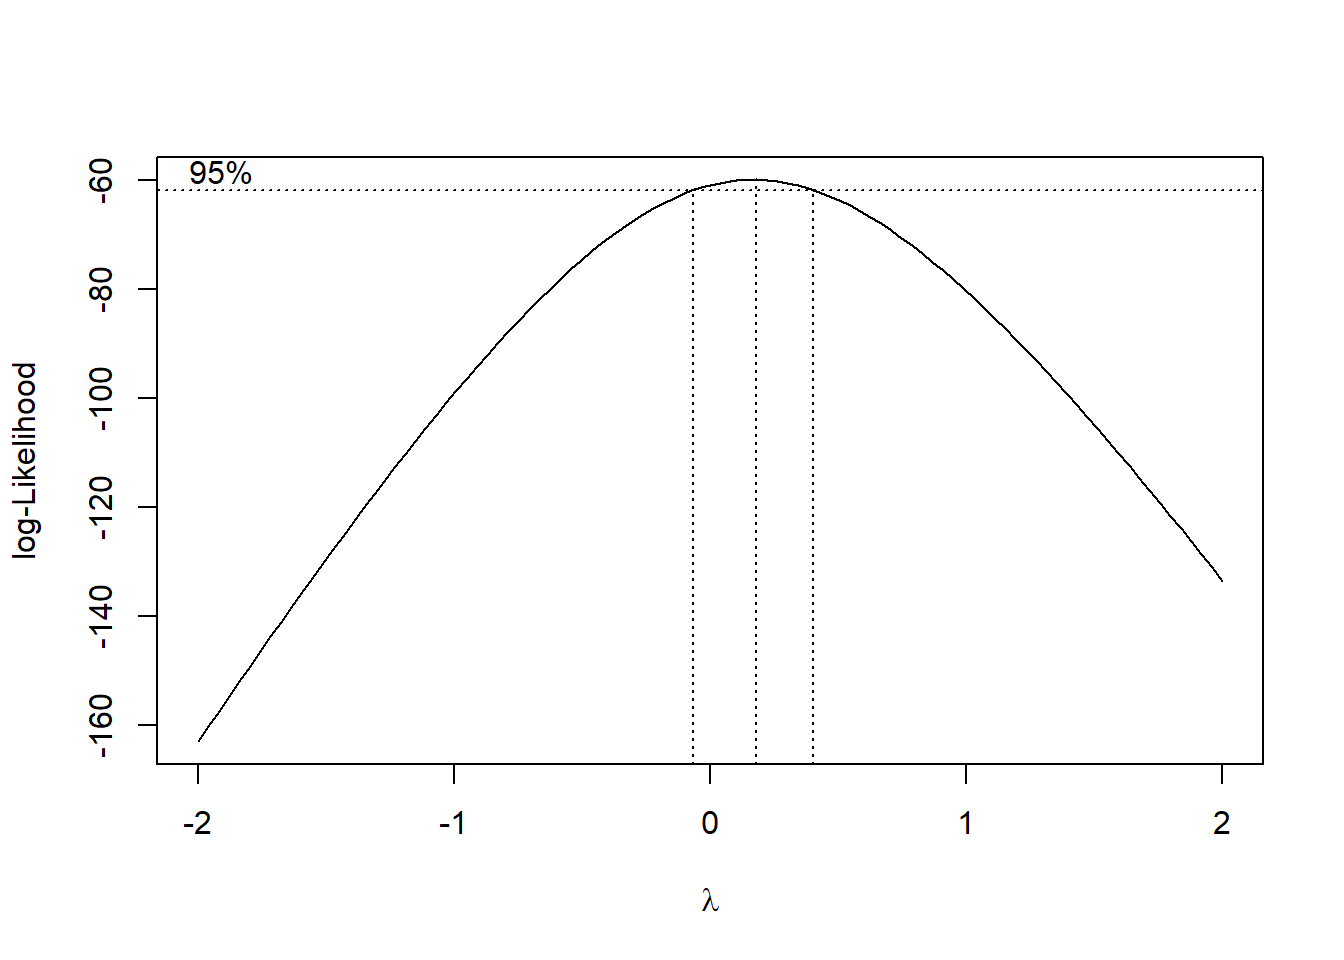
\includegraphics{bookdown-demo_files/figure-latex/unnamed-chunk-165-1.pdf}

A log transformation is preferred if possible, since we can still interpret coefficients. Since 0 lies in the CI, we choose \(\lambda = 0\), to log transform the response variable to get \(y^* = \log(y)\). We regress \(y^*\) against \(x\), and check the resulting residual plot:

\begin{Shaded}
\begin{Highlighting}[]
\DocumentationTok{\#\#log transform response and add to dataframe}
\NormalTok{Data}\SpecialCharTok{$}\NormalTok{y.star}\OtherTok{\textless{}{-}}\FunctionTok{log}\NormalTok{(Data}\SpecialCharTok{$}\NormalTok{Species)}
\DocumentationTok{\#\#perform new regression}
\NormalTok{result.ystar}\OtherTok{\textless{}{-}}\FunctionTok{lm}\NormalTok{(y.star}\SpecialCharTok{\textasciitilde{}}\NormalTok{Area, }\AttributeTok{data=}\NormalTok{Data)}
\FunctionTok{par}\NormalTok{(}\AttributeTok{mfrow =} \FunctionTok{c}\NormalTok{(}\DecValTok{2}\NormalTok{, }\DecValTok{2}\NormalTok{))}
\FunctionTok{plot}\NormalTok{(result.ystar)}
\end{Highlighting}
\end{Shaded}

\includegraphics{bookdown-demo_files/figure-latex/unnamed-chunk-166-1.pdf}

We need to reassess assumptions 1 and 2 after the transformation.

\begin{itemize}
\item
  For assumption 2, we see that the vertical spread of the residuals in the residual plot (top left) is fairly constant, as we move from left to right. So assumption 2 is met. The log transformation worked in stabilizing the variance.
\item
  However, the residual plot still appears to be nonlinear. So assumption 1 is still not met.
\end{itemize}

\hypertarget{transformation-on-x}{%
\subsubsection*{Transformation on x}\label{transformation-on-x}}
\addcontentsline{toc}{subsubsection}{Transformation on x}

To see which specific transformation on the predictor to use, we create a scatterplot of the transformed response and the predictor.

\begin{Shaded}
\begin{Highlighting}[]
\NormalTok{ggplot2}\SpecialCharTok{::}\FunctionTok{ggplot}\NormalTok{(Data, }\FunctionTok{aes}\NormalTok{(}\AttributeTok{x=}\NormalTok{Area,}\AttributeTok{y=}\NormalTok{y.star))}\SpecialCharTok{+}
  \FunctionTok{geom\_point}\NormalTok{()}\SpecialCharTok{+}
  \FunctionTok{geom\_smooth}\NormalTok{(}\AttributeTok{method =} \StringTok{"lm"}\NormalTok{, }\AttributeTok{se=}\ConstantTok{FALSE}\NormalTok{)}\SpecialCharTok{+}
  \FunctionTok{labs}\NormalTok{(}\AttributeTok{x=}\StringTok{"Area of Island (sq km)"}\NormalTok{, }\AttributeTok{y=}\StringTok{"Log \# of Plant Species"}\NormalTok{, }
       \AttributeTok{title=}\StringTok{"Scatterplot of Log Number of Plant Species against Area of Galapagos Island"}\NormalTok{)}
\end{Highlighting}
\end{Shaded}

\includegraphics{bookdown-demo_files/figure-latex/unnamed-chunk-167-1.pdf}

This plot resembles a logarithmic curve, so we use a log transformation on the predictor, so let \(x^{*} = \log(x)\). As usual, a log transformation is preferred since we can still interpret the regression coefficients. We then perform a regression using both the log transformed response variable and predictor, and assess the diagnostic plots.

\begin{Shaded}
\begin{Highlighting}[]
\DocumentationTok{\#\#log transform predictor and add to dataframe}
\NormalTok{Data}\SpecialCharTok{$}\NormalTok{x.star}\OtherTok{\textless{}{-}}\FunctionTok{log}\NormalTok{(Data}\SpecialCharTok{$}\NormalTok{Area)}

\DocumentationTok{\#\#perform new regression}
\NormalTok{result.xystar}\OtherTok{\textless{}{-}}\FunctionTok{lm}\NormalTok{(y.star}\SpecialCharTok{\textasciitilde{}}\NormalTok{x.star, }\AttributeTok{data=}\NormalTok{Data)}
\FunctionTok{par}\NormalTok{(}\AttributeTok{mfrow =} \FunctionTok{c}\NormalTok{(}\DecValTok{2}\NormalTok{, }\DecValTok{2}\NormalTok{))}
\FunctionTok{plot}\NormalTok{(result.xystar)}
\end{Highlighting}
\end{Shaded}

\includegraphics{bookdown-demo_files/figure-latex/unnamed-chunk-168-1.pdf}

Based on the residual plot (top left), both assumptions are met. The residuals are evenly scattered across the horizontal axis with no pattern. The vertical spread of the residuals is also constant. So the transformations worked.

\hypertarget{interpreting-coefficients-with-log-transformed-response-and-predictor}{%
\subsubsection*{Interpreting Coefficients with Log Transformed Response and Predictor}\label{interpreting-coefficients-with-log-transformed-response-and-predictor}}
\addcontentsline{toc}{subsubsection}{Interpreting Coefficients with Log Transformed Response and Predictor}

So our regression equation is

\begin{Shaded}
\begin{Highlighting}[]
\NormalTok{result.xystar}
\end{Highlighting}
\end{Shaded}

\begin{verbatim}
## 
## Call:
## lm(formula = y.star ~ x.star, data = Data)
## 
## Coefficients:
## (Intercept)       x.star  
##      2.9037       0.3886
\end{verbatim}

\(\hat{y^*} = 2.9037 + 0.3886x^{*}\), where \(y^* = \log(y)\) and \(x^* = \log(x)\). There are a couple of ways to interpret the slope:

\begin{itemize}
\item
  For a 1\% increase in the area of a Galapagos island, the number of plant species found on the island is multiplied by \((1.01)^{0.3886} = 1.003874\), OR
\item
  For a 1\% increase in the area of a Galapagos island, the number of plant species increases by about 0.3886\%.
\end{itemize}

\hypertarget{mlr}{%
\chapter{Multiple Linear Regression (MLR)}\label{mlr}}

\hypertarget{introduction-5}{%
\section{Introduction}\label{introduction-5}}

Linear regression models are used to explore the relationship between variables as well as make predictions. Simple linear regression (SLR) concerns the study of only one predictor variable with one response variable. However, given the context, it may be clear there are multiple predictors that relate to the response variable. In such a context, we want to:

\begin{itemize}
\tightlist
\item
  Improve predictions on the response variable by including more useful predictors.
\item
  Assess how a predictor relates to the response variable when controlling for other predictors.
\end{itemize}

\textbf{Multiple linear regression (MLR)} models allow us to examine the effect of multiple predictors on the response variable simultaneously.

There are a couple of ways to think about MLR:

\begin{itemize}
\tightlist
\item
  Extension of SLR to MLR.
\item
  SLR as a special case of MLR.
\end{itemize}

As a motivating example, we look at data regarding black cherry trees. The data, \texttt{cherry} come from the \texttt{openintro} package. Researchers want to understand the relationship between the volume of these trees and their diameter and height. Data come from 31 trees in the Allegheny National Forest, Pennsylvania.

\begin{Shaded}
\begin{Highlighting}[]
\FunctionTok{library}\NormalTok{(openintro)}
\NormalTok{Data}\OtherTok{\textless{}{-}}\NormalTok{openintro}\SpecialCharTok{::}\NormalTok{cherry}
\end{Highlighting}
\end{Shaded}

From this context, we know that volume of a tree is influenced by its diameter and height, so we have more than one predictor in this study.

As you read this set of notes, take note of the similarities and differences between SLR and MLR.

\hypertarget{notation-in-mlr}{%
\section{Notation in MLR}\label{notation-in-mlr}}

We write the \textbf{MLR model} as:

\begin{equation} 
y_i = \beta_0+\beta_1 x_{i1} + \beta_2 x_{i2} + \cdots + \beta_{k} x_{i k} + \epsilon_i.
\label{eq:6MLRmod}
\end{equation}

In this setup, we have \(k\) quantitative predictors. The notation in \eqref{eq:6MLRmod} are as follows:

\begin{itemize}
\tightlist
\item
  \(y_i\): value of response variable for observation \(i\),
\item
  \(\beta_0\): \textbf{intercept} for MLR model,
\item
  \(\beta_j\): \textbf{coefficient} (or slope) for predictor \(j\), for \(j = 1, 2, \cdots, k\). We have \(k\) predictors, each with its corresponding coefficient.
\item
  \(x_{ij}\): observation \(i\)'s value for predictor \(j\). Notice there are two numbers in the subscript. The first number denotes which observation, and the second denotes which predictor.
\item
  \(\epsilon_i:\) \textbf{error} for observation \(i\).
\end{itemize}

The \textbf{assumptions} in MLR are identical to SLR:

\begin{equation} 
\epsilon_1,\ldots,\epsilon_n \ i.i.d. \sim N(0,\sigma^2).
\label{eq:6assumptions}
\end{equation}

Let us use the \texttt{cherry} data from \texttt{openintro} as an example:

\begin{Shaded}
\begin{Highlighting}[]
\FunctionTok{head}\NormalTok{(Data)}
\end{Highlighting}
\end{Shaded}

\begin{verbatim}
## # A tibble: 6 x 3
##    diam height volume
##   <dbl>  <int>  <dbl>
## 1   8.3     70   10.3
## 2   8.6     65   10.3
## 3   8.8     63   10.2
## 4  10.5     72   16.4
## 5  10.7     81   18.8
## 6  10.8     83   19.7
\end{verbatim}

\begin{itemize}
\tightlist
\item
  \(y_2\) = 10.3 cubic feet, the volume for observation 2
\item
  \(x_{41} = 10.5\) inches, observation 4's diameter (predictor 1)
\item
  \(x_{22} = 65\) feet, observation 2's height (predictor 2)
\end{itemize}

The MLR model in \eqref{eq:6MLRmod} is often expressed using matrices, which is a lot neater:

\[
\left[
\begin{array}{c}
   y_1  \\
   y_2  \\
   \vdots   \\
   y_n
\end{array}
\right] =
\left[
\begin{array}{cccc}
   1 & x_{11} & \cdots & x_{1k}  \\
   1 & x_{21} & \cdots & x_{2k}  \\
   \vdots   \\
   1 & x_{n1} & \cdots & x_{nk}  \\
\end{array}
\right]
\left[
\begin{array}{c}
\beta_0 \\
\beta_1 \\
\vdots \\
\beta_{k}
\end{array}
\right] +
\left[
\begin{array}{c}
   \epsilon_1  \\
   \epsilon_2  \\
   \vdots   \\
   \epsilon_n
\end{array}
\right],
\]

or

\begin{equation} 
\boldsymbol{y} = \boldsymbol{X \beta} + \boldsymbol{\epsilon}.
\label{eq:6matrix}
\end{equation}

The notation in \eqref{eq:6matrix} are as follows:

\begin{itemize}
\tightlist
\item
  \(\boldsymbol{y}\): \textbf{vector of responses} (length \(n\)),
\item
  \(\boldsymbol{\beta}\): \textbf{vector of parameters} (length \(p = k+1\), where \(p\) denotes the number of regression parameters),
\item
  \(\boldsymbol{X}\): \textbf{design matrix} (dimension \(n \times p\)),
\item
  \(\boldsymbol{\epsilon}\): \textbf{vector of residuals} (length \(n\)).
\end{itemize}

The formulation in \eqref{eq:6matrix} is the basis for calling the model a ``linear'' regression. The model is \textbf{linear in the parameters}, not the predictors. A common misconception is that the model is linear in the predictors.

Following \eqref{eq:6MLRmod}, the \textbf{MLR equation} can be written as:

\begin{equation} 
E(y|x) = \beta_0+\beta_1 x_1 + \beta_2 x_2 + \cdots + \beta_{k} x_k.
\label{eq:6MLR}
\end{equation}

And in turn, the \textbf{estimated MLR equation} can be written as:

\begin{equation} 
\hat{y} = \hat{\beta_0}+\hat{\beta_1} x_1 + \hat{\beta_2} x_2 + \cdots + \hat{\beta_{k}} x_k.
\label{eq:6MLReq}
\end{equation}

\hypertarget{interpreting-coefficients-in-mlr}{%
\subsection{Interpreting coefficients in MLR}\label{interpreting-coefficients-in-mlr}}

The interpretation of estimated coefficients are similar with SLR, with a small caveat: \(\hat{\beta}_j\) denotes the change in the predicted response per unit change in \(x_j\), \textbf{when the other predictors are held constant.} There are other common ways to state the bold part:

\begin{itemize}
\tightlist
\item
  when controlling for the other predictors.
\item
  when the other predictors are taken into account.
\item
  after adjusting for the effect of the other predictors.
\end{itemize}

If you are familiar with how a partial derivative is interpreted in multivariate calculus, you will realize that the interpretation of estimated coefficients in MLR sound like how a partial derivative is interpreted.

Let us look at the estimated regression equation for the \texttt{cherry} data:

\begin{Shaded}
\begin{Highlighting}[]
\NormalTok{result}\OtherTok{\textless{}{-}}\FunctionTok{lm}\NormalTok{(volume}\SpecialCharTok{\textasciitilde{}}\NormalTok{., }\AttributeTok{data=}\NormalTok{Data)}
\NormalTok{result}
\end{Highlighting}
\end{Shaded}

\begin{verbatim}
## 
## Call:
## lm(formula = volume ~ ., data = Data)
## 
## Coefficients:
## (Intercept)         diam       height  
##    -57.9877       4.7082       0.3393
\end{verbatim}

The estimated MLR equation is \(\hat{y} = -57.9877 + 4.7082x_1 + 0.3393x_2\). The estimated coefficient for diameter inform us that for each additional inch in diameter, the predicted volume of a cherry tree increases by 4.7082 cubic feet, while holding height constant.

\hypertarget{visualizing-mlr}{%
\subsection{Visualizing MLR}\label{visualizing-mlr}}

How should we visualize an MLR equation? Suppose we have two predictor variables, \(x_1\) and \(x_2\), with MLR equation \(E(y|x_1,x_2) = 2 + 5x_1 + 5x_2\). A \textbf{contour plot} can be used to visualize a response variable with two predictors:

\includegraphics{bookdown-demo_files/figure-latex/unnamed-chunk-174-1.pdf}

The contour plot creates an axis for each predictor. The value of the response variable is denoted by the contour lines with the actual value displayed on the line. In this toy example, \(\beta_1 = 5\). This means that if we hold \(x_2\) constant (e.g.~set \(x_2 = 1\) per the red horizontal line), increasing \(x_1\) by 1 unit increases the mean of \(y\) by 5 units.

The regression equation \(E(y|x_1,x_2) = 2 + 5x_1 + 5x_2\) is sometimes called a \textbf{regression plane}, instead of a regression line, since we have more than 1 predictor. We can visualize this regression plane below

\includegraphics{images/3dplot.jpg}

Due to limitations in human visualization, going beyond a 3-dimensional plot (1 response and 2 predictors) is difficult.

\emph{Please see the associated video for a little more explanation regarding the contour plot and 3-dimensional plot}.

\hypertarget{estimating-coefficients-in-mlr}{%
\section{Estimating coefficients in MLR}\label{estimating-coefficients-in-mlr}}

From \eqref{eq:6MLReq}, the predicted response (or fitted values), can be written in matrix form as:

\begin{equation} 
\boldsymbol{\hat{y}} = \boldsymbol{X\hat{\beta}},
\label{eq:6yhat}
\end{equation}

where \(\boldsymbol{\hat{\beta}} = (\hat{\beta_0}, \hat{\beta_1}, \cdots, \hat{\beta_k})^\prime\).

We use the \textbf{method of least squares} to find the estimated coefficients in MLR. This is the same idea when applied in SLR. The method involves minimizing the \textbf{sum of squared residuals}, \(SS_{res}\). In SLR, we minimize

\[
\sum\limits_{i=1}^{n} \left[ y_i - (\hat{\beta_0}+\hat{\beta_1} x_i) \right]^{2}
\]

with respect to \(\hat{\beta_0}, \hat{\beta_1}\). In MLR, the \(SS_{res}\) can be expressed in matrix form:

\begin{equation}
Q = \left(\boldsymbol{y - X\hat{\beta}}\right)^{\prime} \left(\boldsymbol{y - X\hat{\beta}}\right)
\label{eq:6min}
\end{equation}

To minimize the \(Q = SS_{res}\) with respect to \(\hat{\beta_0}, \hat{\beta_1}, \cdots, \hat{\beta_k}\), We take partial derivatives of \(Q\) and set them all to 0, i.e.~\(\frac{\nabla Q}{\nabla \hat{\beta}}=0\). Solving for these equations, we get

\begin{equation} 
\boldsymbol{\hat{\beta}} = \left[
\begin{array}{c}
   \hat{\beta}_0  \\
   \hat{\beta}_1 \\
   \vdots \\
   \hat{\beta}_k
\end{array}
\right]  =
\left(\boldsymbol{X}^{\prime} \boldsymbol{X} \right)^{-1} \boldsymbol{X}^{\prime} \boldsymbol{y} .
\label{eq:6b}
\end{equation}

\textbf{Residuals} are found in the same way in SLR:

\[
e_i = y_i - \hat{y_i},
\]

or in matrix form:

\begin{equation} 
\boldsymbol{e} = \boldsymbol{y} - \boldsymbol{\hat{y}} = \boldsymbol{y} - \boldsymbol{X\hat{\beta}}.
\label{eq:6res}
\end{equation}

\hypertarget{estimating-variance-of-errors}{%
\subsection{Estimating variance of errors}\label{estimating-variance-of-errors}}

Similar to SLR, \(MS_{res}\) is used to estimate \(\sigma^2\), the variance of the error terms. \(MS_{res}\) if found using

\begin{equation}
MS_{res}=\frac{SS_{res}}{n-p},
\label{eq:6MSres}
\end{equation}

where \(p\) denotes the \textbf{number of regression parameters}. In SLR, \(p=2\), since we have an intercept and one slope. Note: I have seen too many people think \(p\) denotes the number of predictors. This is incorrect! As we move forward, we will explore more complicated regression models and we always think in terms of number of regression parameters.

\hypertarget{distribution-of-least-squares-estimators-1}{%
\subsection{Distribution of least squares estimators}\label{distribution-of-least-squares-estimators-1}}

Following the Gauss Markov theorem, the least squares estimators \(\boldsymbol{\hat{\beta}}\) are unbiased, i.e.

\begin{equation} 
\boldsymbol{E\left(\hat{\beta}\right)} = \boldsymbol{\beta},
\label{eq:6mean2}
\end{equation}

with \textbf{variance-covariance matrix} given by

\begin{equation} 
\boldsymbol{Var}\left(\boldsymbol{\hat{\beta}}\right) = \sigma^{2}\left(\boldsymbol{X^{\prime}X} \right)^{-1}
\label{eq:6cov2}
\end{equation}

with \(\sigma^{2}\) estimated by \(MS_{res}\). A few notes about the variance-covariance matrix of the least squares estimators:

\begin{itemize}
\tightlist
\item
  it is of dimension \(p \times p\),
\item
  the diagonal elements denote the variance of each estimated parameter. For example, the first diagonal element denotes the variance of \(\hat{\beta}_0\), the first estimated parameter.
\item
  the off-diagonal elements denote the covariance between respective parameters. For example, the (1,2) entry denotes the covariance between \(\hat{\beta}_0\) and \(\hat{\beta}_1\).
\end{itemize}

\emph{Please see the associated video for a demonstration on how to read a variance-covariance matrix.}

\hypertarget{anova-f-test-in-mlr}{%
\section{\texorpdfstring{ANOVA \(F\) Test in MLR}{ANOVA F Test in MLR}}\label{anova-f-test-in-mlr}}

\hypertarget{sum-of-squares-1}{%
\subsection{Sum of squares}\label{sum-of-squares-1}}

As in simple regression, the \textbf{analysis of variance (ANOVA) table} for an MLR model displays quantities that measure how much of the variability in the response variable is explained (and not explained) by the regression model. The underlying conceptual idea for the construction of the analysis of variance table is the same:

\begin{equation} 
SS_T = SS_R + SS_{res}.
\label{eq:6SS}
\end{equation}

What change are the associated degrees of freedom:

\begin{itemize}
\tightlist
\item
  df for \(SS_R\): \(df_R = p-1\)
\item
  df for \(SS_{res}\): \(df_{res} = n-p\)
\item
  df for \(SS_T\): \(df_T = n-1\)
\end{itemize}

Notice the degrees of freedom in SLR has \(p=2\).

\hypertarget{anova-table-2}{%
\subsection{ANOVA table}\label{anova-table-2}}

The ANOVA table is thus

\begin{longtable}[]{@{}
  >{\centering\arraybackslash}p{(\columnwidth - 8\tabcolsep) * \real{0.2353}}
  >{\centering\arraybackslash}p{(\columnwidth - 8\tabcolsep) * \real{0.2941}}
  >{\centering\arraybackslash}p{(\columnwidth - 8\tabcolsep) * \real{0.1569}}
  >{\centering\arraybackslash}p{(\columnwidth - 8\tabcolsep) * \real{0.1569}}
  >{\centering\arraybackslash}p{(\columnwidth - 8\tabcolsep) * \real{0.1569}}@{}}
\toprule\noalign{}
\begin{minipage}[b]{\linewidth}\centering
Source of Variation
\end{minipage} & \begin{minipage}[b]{\linewidth}\centering
SS
\end{minipage} & \begin{minipage}[b]{\linewidth}\centering
df
\end{minipage} & \begin{minipage}[b]{\linewidth}\centering
MS
\end{minipage} & \begin{minipage}[b]{\linewidth}\centering
F
\end{minipage} \\
\midrule\noalign{}
\endhead
\bottomrule\noalign{}
\endlastfoot
Regression & \(SS_R=\sum\left(\hat{y_i}-\bar{y}\right)^2\) & \(df_R = p-1\) & \(MS_R=\frac{SS_R}{df_R}\) & \(\frac{MS_R}{MS_{res}}\) \\
Error & \(SS_{res} = \sum\left(y_i-\hat{y_i}\right)^2\) & \(df_{res} = n-p\) & \(MS_{res}=\frac{SS_{res}}{df_{res}}\) & \texttt{***} \\
Total & \(SS_T=\sum\left(y_i-\bar{y}\right)^2\) & \(df_T = n-1\) & \texttt{***} & \texttt{***} \\
\end{longtable}

\hypertarget{anova-f-test-1}{%
\subsection{\texorpdfstring{ANOVA \(F\) test}{ANOVA F test}}\label{anova-f-test-1}}

The null and alternative hypotheses associated with the ANOVA \(F\) test are:

\[
H_0: \beta_1=\beta_2=...=\beta_{k}=0, H_a: \text{ at least one of the coefficients is not 0.}
\]
So the null hypothesis states the regression coefficients for all predictors are 0. Notice how this statement simplifies in SLR.

There are a few different ways to view these hypothesis statements:

\begin{itemize}
\tightlist
\item
  Is our MLR model \textbf{useful}?
\item
  Is our MLR model \textbf{preferred} over an intercept-only model?
\item
  Can we drop \textbf{all} our predictors from the MLR model?
\end{itemize}

The test statistic is still

\begin{equation}
F = \frac{MS_R}{MS_{res}}
\label{eq:6ANOVA}
\end{equation}

which is compared with an \(F_{p-1,n-p}\) distribution.

\hypertarget{coefficient-of-determination-1}{%
\subsection{Coefficient of determination}\label{coefficient-of-determination-1}}

The \textbf{coefficient of determination, \(R^2\),} is still

\begin{equation} 
R^{2} = \frac{SS_R}{SS_T} = 1 - \frac{SS_{res}}{SS_T},
\label{eq:6R2}
\end{equation}

where \(R^{2}\) is interpreted as \textbf{the proportion of variance in the response variable that is explained by the predictors}.

\hypertarget{caution-with-r2}{%
\subsubsection{\texorpdfstring{Caution with \(R^2\)}{Caution with R\^{}2}}\label{caution-with-r2}}

Adding more predictors to a model can only increase \(R^2\), as \(SS_{res}\) never becomes larger with more predictors and \(SS_T\) remains the same for a given set of responses.

\begin{itemize}
\tightlist
\item
  So even adding predictors that don't make sense will increase \(R^2\).
\item
  \(R^2\) should be used to compare models with the same number of parameters.
\item
  \(R^2\) is a popular measure as it has a nice geometric interpretation.
\end{itemize}

In response to this caution, we have the \textbf{adjusted \(R^2\)}, denoted by \(R_{a}^{2}\):

\begin{equation} 
R_{a}^{2} = 1 - \frac{\frac{SS_{res}}{n-p}}{\frac{SS_T}{n-1}} = 1 - \left(\frac{n-1}{n-p} \right) \frac{SS_{res}}{SS_T}.
\label{eq:6adjusted}
\end{equation}

\(R_{a}^{2}\) increases if the added predictors significantly improve the fit of the model, and decreases otherwise.

Let us go back to the \texttt{cherry} dataset as an example:

\begin{Shaded}
\begin{Highlighting}[]
\FunctionTok{summary}\NormalTok{(result)}
\end{Highlighting}
\end{Shaded}

\begin{verbatim}
## 
## Call:
## lm(formula = volume ~ ., data = Data)
## 
## Residuals:
##     Min      1Q  Median      3Q     Max 
## -6.4065 -2.6493 -0.2876  2.2003  8.4847 
## 
## Coefficients:
##             Estimate Std. Error t value Pr(>|t|)    
## (Intercept) -57.9877     8.6382  -6.713 2.75e-07 ***
## diam          4.7082     0.2643  17.816  < 2e-16 ***
## height        0.3393     0.1302   2.607   0.0145 *  
## ---
## Signif. codes:  0 '***' 0.001 '**' 0.01 '*' 0.05 '.' 0.1 ' ' 1
## 
## Residual standard error: 3.882 on 28 degrees of freedom
## Multiple R-squared:  0.948,  Adjusted R-squared:  0.9442 
## F-statistic:   255 on 2 and 28 DF,  p-value: < 2.2e-16
\end{verbatim}

The ANOVA \(F\) statistic is 255` with a small p-value. So we reject the null hypothesis and state that our MLR model with diameter and height as predictors is useful.

The \(R^2\) is 0.948. About 94.8\% of the variance in volume of cherry trees can be explained by their diameter and height.

The \(R_{a}^{2}\) is 0.9442. This value is used in comparison with another model to decide which should be preferred.

\hypertarget{t-test-for-regression-coefficient-in-mlr}{%
\section{\texorpdfstring{\(t\) Test for Regression Coefficient in MLR}{t Test for Regression Coefficient in MLR}}\label{t-test-for-regression-coefficient-in-mlr}}

We can assess whether a regression coefficient is significantly different from 0 in an MLR. The null and alternative hypotheses are very much the same as in SLR:

\[
H_0: \beta_j = 0, H_a: \beta_j \neq 0.
\]
What these hypotheses mean in words:

\begin{itemize}
\tightlist
\item
  The null hypothesis supports dropping predictor \(x_j\) from the MLR model, \textbf{in the presence of the other predictors.}
\item
  The alternative hypothesis supports keeping predictor \(x_j\) in the MLR model, or that we \textbf{cannot drop it in the presence of the other predictors.}
\end{itemize}

Notice the meaning of the null and alternative hypotheses are a little different than in SLR, where other predictors are not taken into account.

The test statistic is still

\begin{equation} 
t = \frac{\hat{\beta}_j}{se(\hat{\beta}_j)}
\label{eq:6ttest}
\end{equation}

which is compared with a \(t_{n-p}\) distribution.

Let us take a look at the \texttt{cherry} dataset:

\begin{Shaded}
\begin{Highlighting}[]
\FunctionTok{summary}\NormalTok{(result)}\SpecialCharTok{$}\NormalTok{coefficients}
\end{Highlighting}
\end{Shaded}

\begin{verbatim}
##                Estimate Std. Error   t value     Pr(>|t|)
## (Intercept) -57.9876589  8.6382259 -6.712913 2.749507e-07
## diam          4.7081605  0.2642646 17.816084 8.223304e-17
## height        0.3392512  0.1301512  2.606594 1.449097e-02
\end{verbatim}

Notice the \(t\) statistics associated with testing for the coefficient for each predictor is highly significant. So we do not have evidence to drop any of the other predictors to simplify the model.

\hypertarget{caution-in-interpretating-t-test-in-mlr}{%
\subsection{\texorpdfstring{Caution in interpretating \(t\) test in MLR}{Caution in interpretating t test in MLR}}\label{caution-in-interpretating-t-test-in-mlr}}

An insignificant \(t\) test for a coefficient \(\beta_j\) in MLR indicates that predictor \(x_j\) can be removed from the model (and leave the other predictors in). It is \textbf{not needed in the presence of the other predictors.}

\begin{enumerate}
\def\labelenumi{\arabic{enumi}.}
\item
  A common misstatement many make is that an insignificant \(t\) test for a coefficient \(\beta_j\) in MLR implies that predictor \(x_j\) has no linear relation with the response variable. This is not necessarily correct!

  \begin{itemize}
  \item
    If \(x_j\) is highly correlated with at least one of the other predictors, or is a linear combination of a number of other predictors, \(x_j\) will probably be insignificant as the addition of \(x_j\) doesn't help in improving the model. This concept is called \textbf{multicollinearity} which we will explore in more depth in the next module. \(x_j\) does not provide independent information from the other predictors, and so will not be needed when the other predictors are in the model.
  \item
    \(x_j\) itself may still be linearly related to the response variable, on its own.
  \item
    If your goal is to assess if \(x_j\) is linearly related to the response, need to use SLR.
  \end{itemize}
\item
  Another common misstatement people make is that if they observe more than one \(t\) statistic that is insignificant, it means that all of the associated predictors can be dropped from the model. This again is not necessarily correct.

  \begin{itemize}
  \tightlist
  \item
    An insignificant \(t\) test informs us we can drop that particular predictor, while leaving the other predictors in the model. We can only drop one predictor at a time based on \(t\) tests.
  \end{itemize}
\end{enumerate}

Notice the limitation of the \(t\) test and ANOVA \(F\) test in MLR:

\begin{itemize}
\tightlist
\item
  We can \textbf{only drop 1 predictor} based on a \(t\) test.
\item
  We can \textbf{drop all predictors} based on an ANOVA \(F\) test.
\item
  What if we wish to drop more than 1 predictor simultaneously, but not all, from the model? We will explore this via another \(F\) test in the next module.
\end{itemize}

\hypertarget{cis-in-mlr}{%
\section{CIs in MLR}\label{cis-in-mlr}}

\hypertarget{ci-for-regression-coefficient}{%
\subsection{CI for regression coefficient}\label{ci-for-regression-coefficient}}

The general form for CIs is still the same:

\begin{equation}
\mbox{estimator} \pm (\mbox{multiplier} \times \mbox{s.e of estimator}). 
\label{eq:6CI}
\end{equation}

The \(100(1-\alpha)\%\) CI for \(\beta_j\) is

\begin{equation} 
\hat{\beta}_j \pm t_{1-\alpha/2;n-p}  se(\hat{\beta}_j) = \hat{\beta}_j \pm t_{1-\alpha/2;n-p} s \sqrt{C_{jj}}
\label{eq:6CIb}
\end{equation}

where \(C_{jj}\) denotes the \(j\)th diagonal entry in variance-covariance matrix of the estimated coefficients, \(\boldsymbol{Var}\left(\boldsymbol{\hat{\beta}}\right)\).

The multiplier is now based on a \(t_{n-p}\) distribution, instead of a \(t_{n-2}\) distribution for SLR.

\hypertarget{ci-of-the-mean-response-1}{%
\subsection{CI of the mean response}\label{ci-of-the-mean-response-1}}

Since we have multiple predictors, we may interested in the CI for the mean of the response, when the predictors are each equal to specific values. Let the vector \(\boldsymbol{x_0}\) denote these values on each predictor, specifically

\[
\boldsymbol{x_0} = (1, x_{01}, x_{02}, \cdots, x_{0k})^{\prime},
\]

where \(x_{0j}\) denotes the value for predictor \(x_j\). The CI for the mean response when \(\boldsymbol{x} = \boldsymbol{x_0}\) is

\begin{equation}
\hat{\mu}_{y|\boldsymbol{x_0}}\pm t_{1-\alpha/2,n-p}s\sqrt{\boldsymbol{x_0}^{\prime} \boldsymbol{(X^\prime X)^{-1}} \boldsymbol{x_0}}.
\label{eq:6CImean}
\end{equation}

\hypertarget{pi-of-a-new-response-1}{%
\subsection{PI of a new response}\label{pi-of-a-new-response-1}}

For a new value of the response when \(\boldsymbol{x} = \boldsymbol{x_0}\), the PI is

\begin{equation} 
\hat{y}_0\pm t_{1-\alpha/2,n-p}s \sqrt{1+ \boldsymbol{x_0}^{\prime} \boldsymbol{(X^\prime X)^{-1}} \boldsymbol{x_0}}.
\label{eq:6pred}
\end{equation}

\hypertarget{r-tutorial-3}{%
\section{R Tutorial}\label{r-tutorial-3}}

For this tutorial, we will learn how to fit multiple linear regression (MLR) in R. You will realize that fitting MLR is very similar to fitting SLR.

We will look at data regarding black cherry trees. The data, \texttt{cherry}, come from the \texttt{openintro} package. Researchers want to understand the relationship between the volume (in cubic feet) of these trees and their diameter (in inches, at 54 inches above ground) and height (in feet). Data come from 31 trees in the Allegheny National Forest, Pennsylvania.

\begin{Shaded}
\begin{Highlighting}[]
\FunctionTok{library}\NormalTok{(openintro)}
\NormalTok{Data}\OtherTok{\textless{}{-}}\NormalTok{openintro}\SpecialCharTok{::}\NormalTok{cherry}
\end{Highlighting}
\end{Shaded}

\hypertarget{scatterplot-matrix}{%
\subsection*{Scatterplot matrix}\label{scatterplot-matrix}}
\addcontentsline{toc}{subsection}{Scatterplot matrix}

A scatterplot matrix is useful to create scatterplots involving more than two quantitative variables. We will use the \texttt{ggpairs()} function from the \texttt{GGally} package:

\begin{Shaded}
\begin{Highlighting}[]
\FunctionTok{library}\NormalTok{(GGally)}
\DocumentationTok{\#\#scatterplot matrix}
\NormalTok{GGally}\SpecialCharTok{::}\FunctionTok{ggpairs}\NormalTok{(Data)}
\end{Highlighting}
\end{Shaded}

\includegraphics{bookdown-demo_files/figure-latex/unnamed-chunk-180-1.pdf}

A few pieces of information are presented in the output. Notice the output is displayed in a matrix format.

\begin{itemize}
\tightlist
\item
  The off-diagonal entries of the output give us the scatterplot and correlation between the corresponding pair of quantitative variables.

  \begin{itemize}
  \tightlist
  \item
    For example, look at the scatterplot in row 3, column 1 of the output. The corresponding label for the column is \texttt{diam} and the label for the row is \texttt{volume}. This informs us this is a scatterplot for \texttt{volume} on the vertical axis and \texttt{diam} on the horizontal axis. We see a strong positive linear association between these two variables.
  \item
    The correlation between \texttt{volume} and \texttt{diam} is displayed in row 1, column 3. Again, notice the label for the column and row. This correlation is 0.967, which is high.
  \item
    For practice, locate the scatterplot of \texttt{volume} and \texttt{height} and its corresponding correlation. Also locate the scatterplot of \texttt{diam} and \texttt{height} and its corresponding correlation.
  \end{itemize}
\item
  The diagonal entries display the density plot of the corresponding variable. For example, the third diagonal entry displays the density plot for \texttt{volume}. We can see that the distribution is somewhat right skewed as most trees have a volume between 10 and 40 cubic feet.
\end{itemize}

\hypertarget{fit-mlr-using-lm}{%
\subsection*{\texorpdfstring{Fit MLR using \texttt{lm()}}{Fit MLR using lm()}}\label{fit-mlr-using-lm}}
\addcontentsline{toc}{subsection}{Fit MLR using \texttt{lm()}}

To fit multiple linear regression (MLR)

\begin{Shaded}
\begin{Highlighting}[]
\DocumentationTok{\#\#Fit MLR model, using + in between predictors}
\NormalTok{result}\OtherTok{\textless{}{-}}\FunctionTok{lm}\NormalTok{(volume}\SpecialCharTok{\textasciitilde{}}\NormalTok{diam}\SpecialCharTok{+}\NormalTok{height, }\AttributeTok{data=}\NormalTok{Data)}
\end{Highlighting}
\end{Shaded}

where we list the predictors after \texttt{\textasciitilde{}} with a \texttt{+} operator in between the predictors. Another way would be

\begin{Shaded}
\begin{Highlighting}[]
\NormalTok{result}\OtherTok{\textless{}{-}}\FunctionTok{lm}\NormalTok{(volume}\SpecialCharTok{\textasciitilde{}}\NormalTok{., }\AttributeTok{data=}\NormalTok{Data)}
\end{Highlighting}
\end{Shaded}

The \texttt{.} after \texttt{\textasciitilde{}} informs the \texttt{lm()} function to use every column other than \texttt{volume} in the data frame as predictors.

Just like with simple linear regression (SLR) we can get relevant information using \texttt{summary()}:

\begin{Shaded}
\begin{Highlighting}[]
\FunctionTok{summary}\NormalTok{(result)}
\end{Highlighting}
\end{Shaded}

\begin{verbatim}
## 
## Call:
## lm(formula = volume ~ diam + height, data = Data)
## 
## Residuals:
##     Min      1Q  Median      3Q     Max 
## -6.4065 -2.6493 -0.2876  2.2003  8.4847 
## 
## Coefficients:
##             Estimate Std. Error t value Pr(>|t|)    
## (Intercept) -57.9877     8.6382  -6.713 2.75e-07 ***
## diam          4.7082     0.2643  17.816  < 2e-16 ***
## height        0.3393     0.1302   2.607   0.0145 *  
## ---
## Signif. codes:  0 '***' 0.001 '**' 0.01 '*' 0.05 '.' 0.1 ' ' 1
## 
## Residual standard error: 3.882 on 28 degrees of freedom
## Multiple R-squared:  0.948,  Adjusted R-squared:  0.9442 
## F-statistic:   255 on 2 and 28 DF,  p-value: < 2.2e-16
\end{verbatim}

\begin{itemize}
\tightlist
\item
  The estimated regression equation is \(\hat{y} = -57.988 + 4.708 diam + 0.339height\).

  \begin{itemize}
  \tightlist
  \item
    The estimated coefficient for \texttt{diam} is interpreted as: the predicted volume of a cherry tree increases by 4.708 cubic feet per inch increase in diameter, while holding height constant.
  \item
    The estimated coefficient for \texttt{height} is interpreted as: the predicted volume of a cherry tree increases by 0.339 cubic feet per foot increase in height, while holding diameter constant.
  \end{itemize}
\item
  The \(R^2\) is 0.948. About 94.8\% of the variance in volume of cherry trees can be explained by their diameter and height.
\item
  The residual standard error is 3.882. This estimates \(\sigma\), the standard deviation of the error term.
\end{itemize}

\hypertarget{inference-with-mlr}{%
\subsection*{Inference with MLR}\label{inference-with-mlr}}
\addcontentsline{toc}{subsection}{Inference with MLR}

Just like SLR, each coefficient is tested against a null hypothesis that \(\beta_j = 0\) with a two-sided alternative. The test is significant for both coefficients, so we cannot drop either predictor from the model.

The ANOVA \(F\) statistic is 255, with a small p-value. So data supports the claim that our model is useful.

The confidence intervals for the coefficients can be found using \texttt{confint()}:

\begin{Shaded}
\begin{Highlighting}[]
\FunctionTok{confint}\NormalTok{(result,}\AttributeTok{level =} \FloatTok{0.95}\NormalTok{)}
\end{Highlighting}
\end{Shaded}

\begin{verbatim}
##                    2.5 %      97.5 %
## (Intercept) -75.68226247 -40.2930554
## diam          4.16683899   5.2494820
## height        0.07264863   0.6058538
\end{verbatim}

The confidence interval for the mean response and the prediction interval for a new observation given a specific value of the predictors can also be found using \texttt{predict()}. For example, when the diameter is 10 inches and height is 80 feet:

\begin{Shaded}
\begin{Highlighting}[]
\NormalTok{newdata}\OtherTok{\textless{}{-}}\FunctionTok{data.frame}\NormalTok{(}\AttributeTok{diam=}\DecValTok{10}\NormalTok{, }\AttributeTok{height=}\DecValTok{80}\NormalTok{)}

\FunctionTok{predict}\NormalTok{(result, newdata, }\AttributeTok{level=}\FloatTok{0.95}\NormalTok{,}
        \AttributeTok{interval=}\StringTok{"confidence"}\NormalTok{)}
\end{Highlighting}
\end{Shaded}

\begin{verbatim}
##        fit      lwr      upr
## 1 16.23404 13.36762 19.10047
\end{verbatim}

\begin{Shaded}
\begin{Highlighting}[]
\FunctionTok{predict}\NormalTok{(result, newdata, }\AttributeTok{level=}\FloatTok{0.95}\NormalTok{,}
        \AttributeTok{interval=}\StringTok{"prediction"}\NormalTok{)}
\end{Highlighting}
\end{Shaded}

\begin{verbatim}
##        fit      lwr      upr
## 1 16.23404 7.781596 24.68649
\end{verbatim}

You might realize by now we are using the same functions as we did in SLR.

\textbf{Note}: Obviously, all these calculations are performed and interpreted assuming the regression assumptions are met. Regression assumptions are checked in the same way as in SLR. On your own, as practice, assess the regression assumptions.

\hypertarget{genF}{%
\chapter{\texorpdfstring{General Linear \(F\) Test and Multicollinearity}{General Linear F Test and Multicollinearity}}\label{genF}}

\hypertarget{introduction-6}{%
\section{Introduction}\label{introduction-6}}

The purpose of multiple linear regression is to use more than one predictor to predict a response variable. This modules explores an approach to choosing which variables to include in a multiple regression model. For example, many variables can be used to predict someone's systolic blood pressure, such as their age, weight, height, and pulse rate. While all of those predictors are likely to influence the systolic blood pressure, we want to know if we need all of them, or if a subset of those predictors will perform just as well. We will use the general linear \(F\) test to do so.

Another issue with having multiple predictors is that the likelihood that at least one of the predictors are linearly dependent, or correlated, with some other predictors increases. This is called multicollinearity. There are some negative consequences if multicollinearity is present. We will learn about these consequences, how to diagnose the presence of multicollinearity, and some solutions if multicollinearity is present.

\hypertarget{the-general-linear-f-test}{%
\section{\texorpdfstring{The General Linear \(F\) Test}{The General Linear F Test}}\label{the-general-linear-f-test}}

\hypertarget{motivation-1}{%
\subsection{Motivation}\label{motivation-1}}

In the previous module, we noted the limitation of the \(t\) test and ANOVA \(F\) test in MLR:

\begin{itemize}
\tightlist
\item
  We can \textbf{only drop 1 predictor} based on a \(t\) test.
\item
  We can \textbf{drop all predictors} based on an ANOVA \(F\) test.
\end{itemize}

What if we wish to drop more than 1 predictor simultaneously, but not all, from the model? We will explore this via the \textbf{general linear \(F\) test}. In fact, the \(t\) test and ANOVA \(F\) test are actually special cases of the general linear \(F\) test.

Let us look at a motivating example, using the dataset \texttt{Peruvian.txt}. The data contains variables relating to blood pressures of Peruvians who have migrated from rural high altitude areas to urban lower altitude areas. The variables are:

\begin{itemize}
\tightlist
\item
  \(y\): Systolic blood pressure
\item
  \(x_1\): Age
\item
  \(x_2\): Years in urban area
\item
  \(x_3\): fraction of life in urban area \((x_1/x_2)\)
\item
  \(x_4\): Weight in kg
\item
  \(x_5\): Height in mm
\item
  \(x_6\): Chin skinfold
\item
  \(x_7\): Forearm skinfold
\item
  \(x_8\): Calf skinfold
\item
  \(x_9\): Resting pulse rate
\end{itemize}

We want to assess how the systolic blood pressure of these migrants may be predicted and related to these predictors.

\begin{Shaded}
\begin{Highlighting}[]
\NormalTok{Data}\OtherTok{\textless{}{-}}\FunctionTok{read.table}\NormalTok{(}\StringTok{"Peruvian.txt"}\NormalTok{, }\AttributeTok{header=}\ConstantTok{TRUE}\NormalTok{,}\AttributeTok{sep=}\StringTok{""}\NormalTok{)}
\FunctionTok{head}\NormalTok{(Data)}
\end{Highlighting}
\end{Shaded}

\begin{verbatim}
##   Systol_BP Age Years fraclife Weight Height Chin Forearm Calf Pulse
## 1       170  21     1 0.047619   71.0   1629  8.0     7.0 12.7    88
## 2       120  22     6 0.272727   56.5   1569  3.3     5.0  8.0    64
## 3       125  24     5 0.208333   56.0   1561  3.3     1.3  4.3    68
## 4       148  24     1 0.041667   61.0   1619  3.7     3.0  4.3    52
## 5       140  25     1 0.040000   65.0   1566  9.0    12.7 20.7    72
## 6       106  27    19 0.703704   62.0   1639  3.0     3.3  5.7    72
\end{verbatim}

Let us fit an MLR with all the predictors and take a look at the \(t\) tests and ANOVA \(F\) test:

\begin{Shaded}
\begin{Highlighting}[]
\NormalTok{result}\OtherTok{\textless{}{-}}\FunctionTok{lm}\NormalTok{(Systol\_BP}\SpecialCharTok{\textasciitilde{}}\NormalTok{., }\AttributeTok{data=}\NormalTok{Data)}
\FunctionTok{summary}\NormalTok{(result)}
\end{Highlighting}
\end{Shaded}

\begin{verbatim}
## 
## Call:
## lm(formula = Systol_BP ~ ., data = Data)
## 
## Residuals:
##      Min       1Q   Median       3Q      Max 
## -12.3443  -6.3972   0.0507   5.7293  14.5257 
## 
## Coefficients:
##               Estimate Std. Error t value Pr(>|t|)    
## (Intercept)  146.81883   48.97099   2.998 0.005526 ** 
## Age           -1.12143    0.32741  -3.425 0.001855 ** 
## Years          2.45538    0.81458   3.014 0.005306 ** 
## fraclife    -115.29384   30.16903  -3.822 0.000648 ***
## Weight         1.41393    0.43097   3.281 0.002697 ** 
## Height        -0.03464    0.03686  -0.940 0.355196    
## Chin          -0.94369    0.74097  -1.274 0.212923    
## Forearm       -1.17085    1.19330  -0.981 0.334613    
## Calf          -0.15867    0.53716  -0.295 0.769809    
## Pulse          0.11455    0.17043   0.672 0.506822    
## ---
## Signif. codes:  0 '***' 0.001 '**' 0.01 '*' 0.05 '.' 0.1 ' ' 1
## 
## Residual standard error: 8.655 on 29 degrees of freedom
## Multiple R-squared:  0.6674, Adjusted R-squared:  0.5641 
## F-statistic: 6.465 on 9 and 29 DF,  p-value: 5.241e-05
\end{verbatim}

Notice the \(t\) tests are insignificant for a lot of the coefficients (the last five). Individually, each \(t\) test is informing us that we can drop that specific predictor, while leaving the other predictors in the model.

An erroneous interpretation is to say collectively, these \(t\) tests inform us we can drop all of these predictors, \(x_5\) to \(x_9\), from the model. This is a misconception.

One idea could be to drop the most insignificant predictor, refit the model, and reassess which predictors are insignificant, and continue dropping the most insignificant predictor and refitting the model until all \(t\) tests are significant. We will end up conducting multiple hypothesis tests to do so. If possible, we should limit the number of hypothesis tests we conduct: the more tests we do, the likelihood of us wrongly rejecting a null hypothesis increases.

This is where the \textbf{general linear \(F\) test} (sometimes called a partial \(F\) test) is used. We can perform one test to assess if we can simultaneously drop multiple predictors from the model.

Based on this output, we consider dropping \(x_5, x_6, x_7, x_8, x_9\) since their \(t\) tests are insignificant.

\hypertarget{setting-up-the-general-linear-f-test}{%
\subsection{\texorpdfstring{Setting up the general linear \(F\) test}{Setting up the general linear F test}}\label{setting-up-the-general-linear-f-test}}

The general linear \(F\) test allows us to assess if multiple predictors can be dropped simultaneously from the model. The associated F statistic measures the change in the \(SS_R\) (or \(SS_{res}\)) with the removal of these predictors from the model. The test is based on the following concepts:

\begin{itemize}
\tightlist
\item
  As long as we have the same response variable, \textbf{\(SS_T\) is constant}, regardless of the model. This is because \(SS_T = \sum(y_i - \bar{y})\). It only involves the response variable.
\item
  \(SS_T = SS_R + SS_{Res}\).
\item
  Each time predictors are added to the model, the \(SS_R\) increases and the \(SS_{Res}\) decreases \textbf{by the same amount}, since \(SS_T\) stays constant.
\end{itemize}

The general linear \(F\) test answers the question: is the change in \(SS_R\) (or change in \(SS_{res}\)) significant with the removal or addition of predictor(s)?

This question can be answered in a framework that compares two models:

\begin{itemize}
\tightlist
\item
  a \textbf{full model}, denoted by \(F\), that uses all predictors under consideration,
\item
  a \textbf{reduced model}, denoted by \(R\), that results if some predictors from the full model are dropped.
\end{itemize}

\hypertarget{hypothesis-statements-1}{%
\subsection{Hypothesis statements}\label{hypothesis-statements-1}}

Based on this framework, the null and alternative hypotheses for the \texttt{Peruvian.txt} dataset is

\[
H_0: \beta_5 = \beta_6 = \beta_7 = \beta_8 = \beta_9 = 0, H_a: \text{ at least one coeff in } H_0 \text{ is not zero}.
\]

In general, the null hypothesis states that the \textbf{parameters of the terms that we wish to drop are all 0.} Therefore, the null hypothesis supports the reduced model, R.

The alternative hypothesis states that we cannot drop all the terms that we wish to drop. Therefore, the alternative hypothesis supports the full model, F.

\hypertarget{test-statistic}{%
\subsection{Test statistic}\label{test-statistic}}

The associated test statistic for the general linear \(F\) test is

\begin{equation} 
F_0=\frac{[SS_R(F)-SS_R(R)]/r}{SS_{res}(F)/(n-p)},
\label{eq:7ssr}
\end{equation}

\textbf{or equivalently}

\begin{equation} 
F_0=\frac{[SS_{res}(R)-SS_{res}(F)]/r}{SS_{res}(F)/(n-p)}.
\label{eq:7sse}
\end{equation}

The test statistic \(F_0\) is compared with an \(F_{r,n-p}\) distribution. The notation is as follows:

\begin{itemize}
\tightlist
\item
  \(SS_R(F)\) denotes the \(SS_R\) of full model,
\item
  \(SS_R(R)\) denotes the \(SS_R\) of reduced model,
\item
  \(r\) denotes number of parameters being dropped/tested,
\item
  \(p\) denotes the number of parameters in the full model,
\item
  \(SS_{res}(F)\) denotes the \(SS_{res}\) of full model,
\item
  \(SS_{res}(R)\) denotes the \(SS_{res}\) of reduced model.
\end{itemize}

Note that the change in \(SS_R\), \(SS_R(F)-SS_R(R)\) is always equal to the change in \(SS_{res}\), \(SS_{res}(R)-SS_{res}(F)\). Therefore, \eqref{eq:7ssr} is always equal to \eqref{eq:7sse}.

\hypertarget{worked-example}{%
\subsection{Worked example}\label{worked-example}}

Let us look at some output for our \texttt{Peruvian.txt} dataset:

\begin{Shaded}
\begin{Highlighting}[]
\NormalTok{reduced}\OtherTok{\textless{}{-}}\FunctionTok{lm}\NormalTok{(Systol\_BP}\SpecialCharTok{\textasciitilde{}}\NormalTok{Age}\SpecialCharTok{+}\NormalTok{Years}\SpecialCharTok{+}\NormalTok{fraclife}\SpecialCharTok{+}\NormalTok{Weight, }\AttributeTok{data=}\NormalTok{Data)}
\FunctionTok{anova}\NormalTok{(reduced,result)}
\end{Highlighting}
\end{Shaded}

\begin{verbatim}
## Analysis of Variance Table
## 
## Model 1: Systol_BP ~ Age + Years + fraclife + Weight
## Model 2: Systol_BP ~ Age + Years + fraclife + Weight + Height + Chin + 
##     Forearm + Calf + Pulse
##   Res.Df    RSS Df Sum of Sq      F Pr(>F)
## 1     34 2629.7                           
## 2     29 2172.6  5    457.12 1.2204 0.3247
\end{verbatim}

\begin{itemize}
\item
  In the output, model 1 has the predictors are \(x_1, x_2, x_3, x_4\), while model 2 has the predictors \(x_1, \cdots, x_9\). So model 1 is the reduced model, and model 2 is the full model.
\item
  We see some information presented in a table. The first line corresponds to model 1, the second line corresponds to model 2.
\item
  Under the column \texttt{RSS}, we have the values for \(SS_{res}\). Admittedly, this can be a bit confusing, but it is not \(SS_R\). So we can see that \(SS_{res}(R) = 2629.7\) and \(SS_{res}(F) = 2172.6\). Note that \(SS_{res}\) is always smaller for the full model, and \(SS_R\) is always larger for the full model.
\item
  Under the column \texttt{Res.DF}, we have the degrees of freedom for the \(SS_{res}\) of that model. In the calculation of the \(F\) statistic, we want the value associated with the full model, 29.
\item
  Under the column \texttt{Df}, we have the number of parameters that we are testing to drop, which is 5.
\item
  Under the column \texttt{Sum\ of\ Sq}, we have the difference in \(SS_{res}\) between both models, \(SS_{res}(R) - SS_{res}(F) = 2629.7 - 2172.6 = 457.12\).
\item
  Under the column \texttt{F}, we have the F statistic, \(F_0 = 1.2204\). We can verify this calculation using \eqref{eq:7sse}, \(F_0 = \frac{(2629.7 - 2172.6)/5}{2172.6/29}\) (with some rounding).
\item
  The p-value of this general linear \(F\) test is reported in the last column. This can be found using:
\end{itemize}

\begin{Shaded}
\begin{Highlighting}[]
\DecValTok{1}\SpecialCharTok{{-}}\FunctionTok{pf}\NormalTok{(}\FloatTok{1.2204}\NormalTok{, }\DecValTok{5}\NormalTok{, }\DecValTok{29}\NormalTok{)}
\end{Highlighting}
\end{Shaded}

\begin{verbatim}
## [1] 0.3247085
\end{verbatim}

The critical value can be found using:

\begin{Shaded}
\begin{Highlighting}[]
\FunctionTok{qf}\NormalTok{(}\DecValTok{1}\FloatTok{{-}0.05}\NormalTok{, }\DecValTok{5}\NormalTok{, }\DecValTok{29}\NormalTok{)}
\end{Highlighting}
\end{Shaded}

\begin{verbatim}
## [1] 2.545386
\end{verbatim}

So we fail to reject the null hypothesis. The data do not support the alternative hypothesis (i.e.~the full model). So we go with the reduced model.

\hypertarget{comparison-of-general-linear-f-test-with-other-hypothesis-tests-in-mlr}{%
\subsection{\texorpdfstring{Comparison of general linear \(F\) test with other hypothesis tests in MLR}{Comparison of general linear F test with other hypothesis tests in MLR}}\label{comparison-of-general-linear-f-test-with-other-hypothesis-tests-in-mlr}}

The \(t\) test and ANOVA \(F\) test in MLR are special cases of the general linear \(F\) test, when \(r=1\) and \(r=p-1\) respectively.

\begin{itemize}
\item
  For the \(t\) test, the reduced model has 1 less term than the full model. The \(F_0\) statistic is compared with an \(F_{1,n-p}\) distribution. It turns out that an \(F_{1,n-p}\) distribution is directly related with a \(t_{n-p}\) distribution, and so the general linear \(F\) test is exactly the same as the \(t\) test when dropping 1 term.
\item
  For the ANOVA \(F\) test. The reduced model drops all the terms and has only the intercept. Some call this the intercept-only model.
\end{itemize}

\hypertarget{alternative-approach-to-general-linear-f-test}{%
\subsection{\texorpdfstring{Alternative approach to general linear \(F\) test}{Alternative approach to general linear F test}}\label{alternative-approach-to-general-linear-f-test}}

There is another way in which the information needed to perform a general linear \(F\) test. This approach is called the \textbf{sequential sums of squares} (sometimes called extra sums of squares). It works on the same principle that every time a predictor is added to the model, the \(SS_R\) of the model increases, and the \(SS_{res}\) decreases by the same amount, since \(SS_T\) is constant. The information is displayed as we add one predictor at a time. Let us define some notation:

\begin{itemize}
\tightlist
\item
  \(SS_R(x_1)\) denotes \(SS_R\) when \(x_1\) is the only predictor in the model.
\item
  \(SS_R(x_1, x_2)\) denotes \(SS_R\) when \(x_1, x_2\) are in the model.
\item
  \(SS_R(x_2|x_1)\) denotes the increase in \(SS_R\) when \(x_2\) is added to the model with \(x_1\) already in it. It is read as \(SS_R\) of \(x_2\) given \(x_1\).
\end{itemize}

Based on this example, \(SS_R(x_2|x_1) = SS_R(x_1, x_2) - SS_R(x_1)\), and so \(SS_R(x_1, x_2) = SS_R(x_1) + SS_R(x_2|x_1)\). Note that \(SS_R(x_2|x_1)\) is not equal to \(SS_R(x_2)\), as the latter denotes \(SS_R\) when \(x_2\) is the only predictor in the model.

Let us see how we can use the sequential sums of squares with the \texttt{Peruvian.txt} dataset:

\begin{Shaded}
\begin{Highlighting}[]
\FunctionTok{anova}\NormalTok{(result)}
\end{Highlighting}
\end{Shaded}

\begin{verbatim}
## Analysis of Variance Table
## 
## Response: Systol_BP
##           Df  Sum Sq Mean Sq F value    Pr(>F)    
## Age        1    0.22    0.22  0.0030  0.956852    
## Years      1   82.55   82.55  1.1019  0.302514    
## fraclife   1 3112.40 3112.40 41.5448 4.728e-07 ***
## Weight     1  706.55  706.55  9.4311  0.004603 ** 
## Height     1    1.68    1.68  0.0224  0.882113    
## Chin       1  297.68  297.68  3.9735  0.055703 .  
## Forearm    1  113.91  113.91  1.5205  0.227440    
## Calf       1   10.01   10.01  0.1336  0.717419    
## Pulse      1   33.84   33.84  0.4518  0.506822    
## Residuals 29 2172.59   74.92                      
## ---
## Signif. codes:  0 '***' 0.001 '**' 0.01 '*' 0.05 '.' 0.1 ' ' 1
\end{verbatim}

The values under the column ``Sum Sq'' give the sequential \(SS_{R}\)s. So,

\begin{itemize}
\tightlist
\item
  for the first line, we have \(SS_{R}(x_1) = 0.22\),
\item
  the second line, we have \(SS_{R}(x_2|x_1) = 82.55\),
\item
  then \(SS_{R}(x_3|x_1, x_2) = 3112.40\),
\item
  and so on for each term,
\item
  finally, \(SS_{R}(x_9|x_1, x_2, \cdots, x_8) = 33.84\).
\item
  The very last line refers to \(SS_{Res}(x_1, x_2, \cdots, x_9) = 2172.59\).
\end{itemize}

Essentially, the output for each term informs us the increase in \(SS_R\) when that term is added to the model, given that the previously listed terms are already in the model.

Notice the order the sequential sums of squares are displayed is the same order used when entering the predictors in \texttt{lm()}.

We are still testing

\[
H_0: \beta_5 = \beta_6 = \beta_7 = \beta_8 = \beta_9 = 0, H_a: \text{ at least one coeff in } H_0 \text{ is not zero}.
\]

Using \eqref{eq:7ssr}, the F statistic for this test is

\(\begin{aligned} F_0 &= \frac{[SS_R(F)-SS_R(R)]/r}{SS_{res}(F)/(n-p)} \\  &= \frac{(1.68+297.68+113.91+10.01+33.84)/5}{2172.59/29}\\  &= 1.220339. \end{aligned}\)

Compare this \(F_0\) statistic using this approach with the example shown in Section 2.5. We have the exact same result (other than rounding).

\emph{Please view the associated video for more explanation on the extra sums of squares approach.}

\hypertarget{practice-questions-3}{%
\subsubsection{Practice questions}\label{practice-questions-3}}

We will use the sequential sums of squares for the \texttt{Peruvian.txt} dataset:

\begin{Shaded}
\begin{Highlighting}[]
\FunctionTok{anova}\NormalTok{(result)}
\end{Highlighting}
\end{Shaded}

\begin{verbatim}
## Analysis of Variance Table
## 
## Response: Systol_BP
##           Df  Sum Sq Mean Sq F value    Pr(>F)    
## Age        1    0.22    0.22  0.0030  0.956852    
## Years      1   82.55   82.55  1.1019  0.302514    
## fraclife   1 3112.40 3112.40 41.5448 4.728e-07 ***
## Weight     1  706.55  706.55  9.4311  0.004603 ** 
## Height     1    1.68    1.68  0.0224  0.882113    
## Chin       1  297.68  297.68  3.9735  0.055703 .  
## Forearm    1  113.91  113.91  1.5205  0.227440    
## Calf       1   10.01   10.01  0.1336  0.717419    
## Pulse      1   33.84   33.84  0.4518  0.506822    
## Residuals 29 2172.59   74.92                      
## ---
## Signif. codes:  0 '***' 0.001 '**' 0.01 '*' 0.05 '.' 0.1 ' ' 1
\end{verbatim}

\begin{enumerate}
\def\labelenumi{\arabic{enumi}.}
\tightlist
\item
  Carry out a general linear \(F\) test to assess if we can drop \(x_7, x_8, x_9\) from the model with all predictors.
\item
  What is the value of \(SS_R(x_1, x_2, x_3)\)?
\item
  What is the value of \(SS_{res}(x_1, x_2, x_3)\)?
\item
  What is the value of \(SS_{res}(x_1, x_2, \cdots, x_8)\)?
\end{enumerate}

\emph{Please view the associated video for a review of these practice questions.}

\hypertarget{multicollinearity}{%
\section{Multicollinearity}\label{multicollinearity}}

What happens if at least one predictor is almost a linear combination of other predictors? This is called multicollinearity, and there are negative consequences on our MLR model. We will learn what these negative consequences are, how to detect multicollinearity, and some solutions. As we consider more and more predictors for our model, multicollinearity is more likely to exist.

\hypertarget{linear-dependency-multicollinearity}{%
\subsection{Linear dependency \& multicollinearity}\label{linear-dependency-multicollinearity}}

Before we define multicollinearity, we have to define linear dependency. Recall that we can write the MLR model in matrix form as

\begin{equation} 
\boldsymbol{y} = \boldsymbol{X \beta} + \boldsymbol{\epsilon}.
\label{eq:7matrix}
\end{equation}

where \(\boldsymbol{X}\) is the design matrix and is

\[
\left[
\begin{array}{cccc}
   1 & x_{11} & \cdots & x_{1k}  \\
   1 & x_{21} & \cdots & x_{2k}  \\
   \vdots   \\
   1 & x_{n1} & \cdots & x_{nk}  \\
\end{array}
\right]
\]

Note that each column of the design matrix (other than column 1) represents each predictor variable.

The columns of a matrix are \textbf{linearly dependent} if at least one column can be expressed as a linear combination of the other columns (there exist nonzero constants \(c_i\) such that \(c_1x_1 + c_2x_2 + ... + c_{k}x_{k} = 0\)).

As an example, suppose we have three predictors: \(x_1\) denoting SAT verbal score, \(x_2\) denoting SAT math score, and \(x_3\) denoting SAT score. Since SAT score is the sum of the SAT verbal and math scores, \(x_3 = x_1 + x_2\). So if we were to create the design matrix for these three predictors, we have linear dependency. With linear dependency, we can predict \(x_3\) from \(x_1, x_2\) with no error. Recall that the least squares estimators are found using

\begin{equation}
\boldsymbol{\hat\beta} = \left(\boldsymbol{X}^{\prime} \boldsymbol{X} \right)^{-1} \boldsymbol{X}^{\prime} \boldsymbol{y}.
\label{eq:7ls}
\end{equation}

If there is a linear dependence among the columns of \(\boldsymbol{X}\), then \(\bf{(X^{\prime}X)}^{-1}\) does not exist. This means that unique estimates of \(\beta_j\)'s cannot be determined.

\textbf{Multicollinearity} exists in our model when at least one predictor is \textbf{almost linearly dependent}, or can be predicted with a high degree of accuracy, from the other predictors.

An example of multicollinearity would be if we have predictors \(x_1\) denoting right arm length, \(x_2\) denoting right thigh length, and \(x_3\) denoting right calf length. If we know someone's right arm and right thigh lengths, we can probably predict their right calf length with a high degree of accuracy. In this example, we are likely to have multicollinearity.

With multiple predictors, we will always find some degree of \textbf{collinearity}. The question is whether this degree is high enough warrant our concern.

When predictors are linearly dependent on each other, they do not provide independent information in their association to the response variable. It becomes difficult to \textbf{separate} their effects on the response variable.

\hypertarget{sources}{%
\subsection{Sources of multicollinearity}\label{sources}}

There are a few reasons for the presence of multicollinearity.

\hypertarget{study-design}{%
\subsubsection{Study design}\label{study-design}}

The design of the study might lead to multicollinearity, and so a solution will be to change its design. Let us consider this example:

Suppose the Virginia Department of Motor Vehicles (DMV) wants to study the waiting time customers spend waiting in line, based on the number of people ahead in line and number of counters open.

\begin{itemize}
\item
  The number of people ahead in line and number of counters open could be highly positively correlated; the more people in line, the more counters will be staffed by the DMV. So the nature of the study leads to multicollinearity.
\item
  To break the multicollinearity between the number of people ahead in line and number of counters open, we could collect data on instances where the number of people in line is high, yet the number of counters opened is low, and vice versa. This will allow us to isolate the effect of each predictor on waiting times.
\end{itemize}

\hypertarget{nature-of-the-data}{%
\subsubsection{Nature of the data}\label{nature-of-the-data}}

Sometimes, the very nature of the variables lead to multicollinearity and we cannot do much to remedy this.

Suppose we wish to investigate electric consumption in households based on income and size of the home in a city.

\begin{itemize}
\item
  Income and size of the home are likely to be highly correlated, due to high income earners wanting to buy bigger homes, and low income earners being unable to buy bigger homes.
\item
  We cannot force high income earners to live in small homes, or have low income earners buy bigger homes to break the multicollinearity. In this setting, we have to choose one of the predictors.
\end{itemize}

\hypertarget{too-many-predictors}{%
\subsubsection{Too many predictors}\label{too-many-predictors}}

As we collect data on more and more variables, we are more likely to encounter multicollinearity. We have to ask if some predictors are provide the same, or similar information, as other predictors.

\hypertarget{consequences-of-multicollinearity}{%
\subsection{Consequences of multicollinearity}\label{consequences-of-multicollinearity}}

The main consequence with multicollinearity is that we have \textbf{high variance with the estimated coefficients}. This means the value of the estimated coefficient may be very different from the true value. The consequences from this are:

\begin{itemize}
\item
  Estimated coefficients can be difficult to interpret, as the estimated value may be different from the true parameter. Also, if 2 predictors are correlated, then holding one constant while increasing the other one may not make much sense.
\item
  Algebraic sign of coefficients can be different from what is known theoretically. If the true coefficient is positive, but because the estimated coefficient is different, it could be negative. So we may think the direction of the association is opposite.
\item
  Predictors that we know should impact the response variable are found to be insignificant, as the standard error of the estimated coefficient is large, and hence the \(t\) statistic is small. We may erroneously think that predictor is not related to the response variable.
\end{itemize}

Interestingly, predictions may still be unbiased if the regression assumptions are met.

So depending on what you are using your regression model for, multicollinearity may or may not be a huge problem. Recall the two main uses of regression models:

\begin{enumerate}
\def\labelenumi{\arabic{enumi}.}
\tightlist
\item
  \textbf{Prediction}: Predict a future value of a response variable, using information from predictor variables.
\item
  \textbf{Association}: Quantify the relationship between variables. How does a change in the predictor variable change the value of the response variable?
\end{enumerate}

\begin{itemize}
\tightlist
\item
  If the goal of your regression analysis is to interpret the coefficients and understand the effects of each the predictors on the response variable, multicollinearity is a big issue.
\item
  If the goal of your regression analysis is predict future values of the response, then multicollinearity may be less of an issue as long as you do not extrapolate.
\end{itemize}

\hypertarget{detecting-multicollinearity}{%
\section{Detecting Multicollinearity}\label{detecting-multicollinearity}}

The following are indicators of the presence of multicollinearity:

\begin{enumerate}
\def\labelenumi{\arabic{enumi}.}
\item
  \textbf{Insignificant} results in individual tests on the regression
  coefficients for important predictor variables. A significant ANOVA F test provides more evidence of multicollinearity.
\item
  The presence of estimated coefficients with \textbf{large standard errors}.
\item
  Estimated regression coefficients with an algebraic sign
  that is the \textbf{opposite} of that expected from theoretical
  considerations or prior experience.
\item
  \textbf{High correlation} between pairs of
  predictor variables.
\item
  \textbf{High variance inflation factors} (VIFs).
\end{enumerate}

We have touched upon the first three ways earlier, and using correlation makes intuitive sense. Next, we will look at VIFs in a bit more detail.

\hypertarget{variance-inflation-factors-vifs}{%
\subsection{Variance inflation factors (VIFs)}\label{variance-inflation-factors-vifs}}

\textbf{Variance inflation factors (VIFs)} are associated with the coefficients of the predictor variables in MLR. VIFs measure \textbf{how much the variance of the corresponding coefficient is multiplied by due to the presence of collinearity versus the lack of collinearity being present}. Mathematically, VIFs are defined as:

\begin{equation}
\left(VIF\right)_j = \frac{1}{1-R_j^2},
\,\,\,\,\,\,j=1,2,\ldots,k,
\label{eq:7vif}
\end{equation}

where \(R_j^2\) is the \textbf{coefficient of determination when
\(x_j\) is regressed on the other \(k-1\) predictors in the model}.

Larger VIFs indicate stronger evidence of multicollinearity. Generally, VIFs greater than 5 indicate some degree of multicollinearity, and VIFs greater than 10 indicate a high level of multicollinearity.

Let us look at the VIFs for the \texttt{Peruvian.txt} dataset:

\begin{Shaded}
\begin{Highlighting}[]
\FunctionTok{library}\NormalTok{(faraway)}
\FunctionTok{round}\NormalTok{(faraway}\SpecialCharTok{::}\FunctionTok{vif}\NormalTok{(result),}\DecValTok{3}\NormalTok{)}
\end{Highlighting}
\end{Shaded}

\begin{verbatim}
##      Age    Years fraclife   Weight   Height     Chin  Forearm     Calf 
##    3.213   34.289   24.387    4.748    1.914    2.064    3.802    2.415 
##    Pulse 
##    1.329
\end{verbatim}

The VIFs for the coefficients for \(x_2, x_3\) are above 5, indicating some degree of multicollinearity in our data.

\hypertarget{handling-multicollinearity}{%
\subsection{Handling multicollinearity}\label{handling-multicollinearity}}

Depends on the source of multicollinearity, as discussed in Section \ref{sources}.

\begin{itemize}
\item
  If due to study design, we can collect data on observations to break the collinearity.
\item
  If due to the nature of the data where some predictors are linearly dependent on others, drop predictor(s). Choose a subset of these predictors (maybe even just one) and remove the rest from the model.
\item
  Abandon least squares regression and use other methods. Other methods such as shrinkage methods and principal components regression help improve predictions, but may not aid in helping explore the relationship between the predictors and response variable. So it depends on what you want to use your regression for.
\end{itemize}

\hypertarget{r-tutorial-4}{%
\section{R Tutorial}\label{r-tutorial-4}}

For this tutorial, we will learn how conduct the general linear \(F\) test as well as to detect the presence of multicollinearity in MLR. We will continue to use the \texttt{Peruvian.txt} dataset. The data contains variables relating to blood pressures of Peruvians who have migrated from rural high altitude areas to urban lower altitude areas. The variables are:

\begin{itemize}
\tightlist
\item
  \(y\): Systolic blood pressure
\item
  \(x_1\): Age
\item
  \(x_2\): Years in urban area
\item
  \(x_3\): fraction of life in urban area \((x_1/x_2)\)
\item
  \(x_4\): Weight in kg
\item
  \(x_5\): Height in mm
\item
  \(x_6\): Chin skinfold
\item
  \(x_7\): Forearm skinfold
\item
  \(x_8\): Calf skinfold
\item
  \(x_9\): Resting pulse rate
\end{itemize}

We want to assess how the systolic blood pressure of these migrants may be predicted and related to these predictors.

Download the data file and read the data in.

\begin{Shaded}
\begin{Highlighting}[]
\NormalTok{Data}\OtherTok{\textless{}{-}}\FunctionTok{read.table}\NormalTok{(}\StringTok{"Peruvian.txt"}\NormalTok{, }\AttributeTok{header=}\ConstantTok{TRUE}\NormalTok{,}\AttributeTok{sep=}\StringTok{""}\NormalTok{)}
\end{Highlighting}
\end{Shaded}

There are a number of strategies on how to start building a multiple linear regression (MLR) model. One possible strategy is to build an initial model based on what appear to be predictors that are most related to the response variable, the systolic blood pressure. Let us create a correlation matrix of the variables:

\begin{Shaded}
\begin{Highlighting}[]
\FunctionTok{round}\NormalTok{(}\FunctionTok{cor}\NormalTok{(Data),}\DecValTok{3}\NormalTok{)}
\end{Highlighting}
\end{Shaded}

\begin{verbatim}
##           Systol_BP    Age  Years fraclife Weight Height   Chin Forearm   Calf
## Systol_BP     1.000  0.006 -0.087   -0.276  0.521  0.219  0.170   0.272  0.251
## Age           0.006  1.000  0.588    0.365  0.432  0.056  0.158   0.055 -0.005
## Years        -0.087  0.588  1.000    0.938  0.481  0.073  0.222   0.143  0.001
## fraclife     -0.276  0.365  0.938    1.000  0.293  0.051  0.120   0.028 -0.113
## Weight        0.521  0.432  0.481    0.293  1.000  0.450  0.562   0.544  0.392
## Height        0.219  0.056  0.073    0.051  0.450  1.000 -0.008  -0.069 -0.003
## Chin          0.170  0.158  0.222    0.120  0.562 -0.008  1.000   0.638  0.516
## Forearm       0.272  0.055  0.143    0.028  0.544 -0.069  0.638   1.000  0.736
## Calf          0.251 -0.005  0.001   -0.113  0.392 -0.003  0.516   0.736  1.000
## Pulse         0.135  0.091  0.237    0.214  0.312  0.008  0.223   0.422  0.209
##           Pulse
## Systol_BP 0.135
## Age       0.091
## Years     0.237
## fraclife  0.214
## Weight    0.312
## Height    0.008
## Chin      0.223
## Forearm   0.422
## Calf      0.209
## Pulse     1.000
\end{verbatim}

We use the \texttt{round()} function so we can limit the number of decimal places the output uses, which in this case is three.

\hypertarget{general-linear-f-test}{%
\subsection*{\texorpdfstring{General Linear \(F\) Test}{General Linear F Test}}\label{general-linear-f-test}}
\addcontentsline{toc}{subsection}{General Linear \(F\) Test}

It appears from the correlation matrix that \(x_3, x_4, x_7, x_8\) have moderately strong linear associations with systolic blood pressure (they have the higest correlations). So we start with these four predictors for our MLR:

\begin{Shaded}
\begin{Highlighting}[]
\DocumentationTok{\#\#fit MLR}
\NormalTok{result}\OtherTok{\textless{}{-}}\FunctionTok{lm}\NormalTok{(Systol\_BP}\SpecialCharTok{\textasciitilde{}}\NormalTok{fraclife}\SpecialCharTok{+}\NormalTok{Weight}\SpecialCharTok{+}\NormalTok{Forearm}\SpecialCharTok{+}\NormalTok{Calf, }\AttributeTok{data=}\NormalTok{Data)}
\FunctionTok{summary}\NormalTok{(result)}
\end{Highlighting}
\end{Shaded}

\begin{verbatim}
## 
## Call:
## lm(formula = Systol_BP ~ fraclife + Weight + Forearm + Calf, 
##     data = Data)
## 
## Residuals:
##      Min       1Q   Median       3Q      Max 
## -17.7706  -7.0950   0.4133   5.8314  24.0159 
## 
## Coefficients:
##              Estimate Std. Error t value Pr(>|t|)    
## (Intercept)  57.11972   15.56936   3.669 0.000827 ***
## fraclife    -27.79798    7.63270  -3.642 0.000892 ***
## Weight        1.33346    0.28858   4.621  5.3e-05 ***
## Forearm      -0.52910    1.14255  -0.463 0.646254    
## Calf         -0.06171    0.60134  -0.103 0.918870    
## ---
## Signif. codes:  0 '***' 0.001 '**' 0.01 '*' 0.05 '.' 0.1 ' ' 1
## 
## Residual standard error: 9.985 on 34 degrees of freedom
## Multiple R-squared:  0.481,  Adjusted R-squared:  0.4199 
## F-statistic: 7.878 on 4 and 34 DF,  p-value: 0.000132
\end{verbatim}

Based on the \(t\) tests, we consider dropping \(x_7, x_8\) from the model. So we perform a general linear \(F\) test with the full model using predictors \(x_3, x_4, x_7, x_8\) and the reduced model only using \(x_3, x_4\). The null and alternative hypotheses are:

\(H_0: \beta_7 = \beta_8 =0\),

\(H_a:\) at least one of the coefficients in \(H_0\) is not 0.

In words, the null hypothesis supports going with the reduced model by dropping \(x_7, x_8\), whereas the alternative hypothesis supports the full model by not dropping \(x_7, x_8\).

We explore two approaches to conducting this general linear \(F\) test.

\hypertarget{directly-comparing-the-full-and-reduced-models}{%
\subsubsection*{Directly comparing the full and reduced models}\label{directly-comparing-the-full-and-reduced-models}}
\addcontentsline{toc}{subsubsection}{Directly comparing the full and reduced models}

In this approach, we fit the reduced model, and then use the \texttt{anova()} function to compare the reduced model with the full model:

\begin{Shaded}
\begin{Highlighting}[]
\NormalTok{reduced}\OtherTok{\textless{}{-}}\FunctionTok{lm}\NormalTok{(Systol\_BP}\SpecialCharTok{\textasciitilde{}}\NormalTok{fraclife}\SpecialCharTok{+}\NormalTok{Weight, }\AttributeTok{data=}\NormalTok{Data)}

\DocumentationTok{\#\#general linear F test to compare reduced model with full model}
\FunctionTok{anova}\NormalTok{(reduced, result)}
\end{Highlighting}
\end{Shaded}

\begin{verbatim}
## Analysis of Variance Table
## 
## Model 1: Systol_BP ~ fraclife + Weight
## Model 2: Systol_BP ~ fraclife + Weight + Forearm + Calf
##   Res.Df    RSS Df Sum of Sq      F Pr(>F)
## 1     36 3441.4                           
## 2     34 3389.8  2    51.598 0.2588 0.7735
\end{verbatim}

The \(F\) statistic from this test is 0.2588, with a p-value of 0.7735. So we fail to reject the null hypothesis, so there is little evidence of supporting the full model. We go with the reduced model over the full model.

\hypertarget{sequential-sums-of-squares}{%
\subsubsection*{Sequential sums of squares}\label{sequential-sums-of-squares}}
\addcontentsline{toc}{subsubsection}{Sequential sums of squares}

In this other approach, we use the \texttt{anova()} function on the full model to obtain the \textbf{sequential sums of squares} associated with the full model:

\begin{Shaded}
\begin{Highlighting}[]
\FunctionTok{anova}\NormalTok{(result)}
\end{Highlighting}
\end{Shaded}

\begin{verbatim}
## Analysis of Variance Table
## 
## Response: Systol_BP
##           Df Sum Sq Mean Sq F value    Pr(>F)    
## fraclife   1  498.1  498.06  4.9957   0.03209 *  
## Weight     1 2592.0 2592.01 25.9984 1.279e-05 ***
## Forearm    1   50.5   50.55  0.5070   0.48129    
## Calf       1    1.0    1.05  0.0105   0.91887    
## Residuals 34 3389.8   99.70                      
## ---
## Signif. codes:  0 '***' 0.001 '**' 0.01 '*' 0.05 '.' 0.1 ' ' 1
\end{verbatim}

The values under the column ``Sum Sq'' give the sequential \(SS_{R}\)s. Notice how the information is provided: in the order in which the predictors were entered into \texttt{lm()}.

The general linear F statistic is

\begin{align}
F &= \frac{[SS_R(F) - SS_R(R)]/r}{SS_{res}(F)/(n-p)} \nonumber \\
  &= \frac{[SS_R(x_3, x_4, x_7, x_8) - SS_R(x_3, x_4)]/2}{SS_{res}(x_3, x_4, x_7, x_8)/(39-5)} \nonumber \\
  &= \frac{SS_R(x_7, x_8 | x_3, x_4)/2}{SS_{res}(x_3, x_4, x_7, x_8)/(39-5)} \nonumber \\
  &= \frac{(50.5+1.0)/2}{3389.8/34} \nonumber \\
  &= 0.2582748
\end{align}

which is similar to the value found in approach 1 (discrepancy due to rounding off in intermediate steps).

The corresponding p-value is

\begin{Shaded}
\begin{Highlighting}[]
\DecValTok{1}\SpecialCharTok{{-}}\FunctionTok{pf}\NormalTok{(}\FloatTok{0.2582748}\NormalTok{,}\DecValTok{2}\NormalTok{,}\DecValTok{34}\NormalTok{)}
\end{Highlighting}
\end{Shaded}

\begin{verbatim}
## [1] 0.7738846
\end{verbatim}

and the critical value is

\begin{Shaded}
\begin{Highlighting}[]
\FunctionTok{qf}\NormalTok{(}\FloatTok{0.95}\NormalTok{,}\DecValTok{2}\NormalTok{,}\DecValTok{34}\NormalTok{)}
\end{Highlighting}
\end{Shaded}

\begin{verbatim}
## [1] 3.275898
\end{verbatim}

So we fail to reject the null hypothesis and go with the reduced model.

\hypertarget{multicollinearity-1}{%
\subsection*{Multicollinearity}\label{multicollinearity-1}}
\addcontentsline{toc}{subsection}{Multicollinearity}

With the presence of multiple predictors, it is often tempting to start by including all the predictors in the model.

\begin{Shaded}
\begin{Highlighting}[]
\DocumentationTok{\#\#fit MLR with all predictors}
\NormalTok{all}\OtherTok{\textless{}{-}}\FunctionTok{lm}\NormalTok{(Systol\_BP}\SpecialCharTok{\textasciitilde{}}\NormalTok{., }\AttributeTok{data=}\NormalTok{Data)}
\end{Highlighting}
\end{Shaded}

There are a few ways to detect the presence of multicollinearity in our model.

\hypertarget{t-tests-and-anova-f-test}{%
\subsubsection*{\texorpdfstring{\(t\) tests and ANOVA \(F\) test}{t tests and ANOVA F test}}\label{t-tests-and-anova-f-test}}
\addcontentsline{toc}{subsubsection}{\(t\) tests and ANOVA \(F\) test}

The presence of a lot of insignificant \(t\) tests for the regression coefficients, along a highly significant ANOVA \(F\) test is an indication that multicollinearity is present:

\begin{Shaded}
\begin{Highlighting}[]
\DocumentationTok{\#\#look at t tests, and F test}
\FunctionTok{summary}\NormalTok{(all)}
\end{Highlighting}
\end{Shaded}

\begin{verbatim}
## 
## Call:
## lm(formula = Systol_BP ~ ., data = Data)
## 
## Residuals:
##      Min       1Q   Median       3Q      Max 
## -12.3443  -6.3972   0.0507   5.7293  14.5257 
## 
## Coefficients:
##               Estimate Std. Error t value Pr(>|t|)    
## (Intercept)  146.81883   48.97099   2.998 0.005526 ** 
## Age           -1.12143    0.32741  -3.425 0.001855 ** 
## Years          2.45538    0.81458   3.014 0.005306 ** 
## fraclife    -115.29384   30.16903  -3.822 0.000648 ***
## Weight         1.41393    0.43097   3.281 0.002697 ** 
## Height        -0.03464    0.03686  -0.940 0.355196    
## Chin          -0.94369    0.74097  -1.274 0.212923    
## Forearm       -1.17085    1.19330  -0.981 0.334613    
## Calf          -0.15867    0.53716  -0.295 0.769809    
## Pulse          0.11455    0.17043   0.672 0.506822    
## ---
## Signif. codes:  0 '***' 0.001 '**' 0.01 '*' 0.05 '.' 0.1 ' ' 1
## 
## Residual standard error: 8.655 on 29 degrees of freedom
## Multiple R-squared:  0.6674, Adjusted R-squared:  0.5641 
## F-statistic: 6.465 on 9 and 29 DF,  p-value: 5.241e-05
\end{verbatim}

Notice how five of the \(t\) tests are insignificant, but the ANOVA \(F\) is highly significant. So we have evidence of multicollinearity.

\hypertarget{standard-errors-of-estimated-coefficients}{%
\subsubsection*{Standard errors of estimated coefficients}\label{standard-errors-of-estimated-coefficients}}
\addcontentsline{toc}{subsubsection}{Standard errors of estimated coefficients}

Looking at the output from \texttt{summary()}, we do not see any standard errors that are large. If we have strong multicollinearity, standard errors should be large.

\hypertarget{correlation-between-pairs-of-predictors}{%
\subsubsection*{Correlation between pairs of predictors}\label{correlation-between-pairs-of-predictors}}
\addcontentsline{toc}{subsubsection}{Correlation between pairs of predictors}

We can also look at the pairwise correlations among predictors:

\begin{Shaded}
\begin{Highlighting}[]
\DocumentationTok{\#\#correlation matrix, round to 3 decimal}
\FunctionTok{round}\NormalTok{(}\FunctionTok{cor}\NormalTok{(Data[,}\SpecialCharTok{{-}}\DecValTok{1}\NormalTok{]),}\DecValTok{3}\NormalTok{)}
\end{Highlighting}
\end{Shaded}

\begin{verbatim}
##             Age Years fraclife Weight Height   Chin Forearm   Calf Pulse
## Age       1.000 0.588    0.365  0.432  0.056  0.158   0.055 -0.005 0.091
## Years     0.588 1.000    0.938  0.481  0.073  0.222   0.143  0.001 0.237
## fraclife  0.365 0.938    1.000  0.293  0.051  0.120   0.028 -0.113 0.214
## Weight    0.432 0.481    0.293  1.000  0.450  0.562   0.544  0.392 0.312
## Height    0.056 0.073    0.051  0.450  1.000 -0.008  -0.069 -0.003 0.008
## Chin      0.158 0.222    0.120  0.562 -0.008  1.000   0.638  0.516 0.223
## Forearm   0.055 0.143    0.028  0.544 -0.069  0.638   1.000  0.736 0.422
## Calf     -0.005 0.001   -0.113  0.392 -0.003  0.516   0.736  1.000 0.209
## Pulse     0.091 0.237    0.214  0.312  0.008  0.223   0.422  0.209 1.000
\end{verbatim}

Looking at this matrix, we notice that pairs of predictors involving \(x_1, x_2, x_3\), and \(x_4, x_6, x_7\) have high correlations. For pairs involving other predictors, the correlations are a lot weaker. So there is some degree of multicollinearity.

\hypertarget{vifs}{%
\subsubsection*{VIFs}\label{vifs}}
\addcontentsline{toc}{subsubsection}{VIFs}

High VIFs are an indication of multicollinearity.

\begin{Shaded}
\begin{Highlighting}[]
\DocumentationTok{\#\#VIFs}
\FunctionTok{library}\NormalTok{(faraway)}
\NormalTok{faraway}\SpecialCharTok{::}\FunctionTok{vif}\NormalTok{(all)}
\end{Highlighting}
\end{Shaded}

\begin{verbatim}
##       Age     Years  fraclife    Weight    Height      Chin   Forearm      Calf 
##  3.213372 34.289220 24.387489  4.747710  1.913992  2.063865  3.802313  2.414603 
##     Pulse 
##  1.329233
\end{verbatim}

The largest VIFs belong to \(x_2\) and \(x_3\), which are 34.289220 and 24.387489 respectively. VIFs above 10 indicate a strong degree of multicollinearity.

To summarize what we have seen:

\begin{itemize}
\tightlist
\item
  The ANOVA F test is significant, but a lot of the t tests are insignificant.
\item
  We don't see huge standard errors for the estimated coefficients.
\item
  Some of the predictors have high pairwise correlations, e.g.~Pairs involving \(x_1, x_2, x_3\), and \(x_4, x_6, x_7\).
\item
  The largest VIF is 34.289220.
\end{itemize}

Collectively, there is some degree of multicollinearity in this model.

\hypertarget{next-steps}{%
\subsubsection*{Next steps}\label{next-steps}}
\addcontentsline{toc}{subsubsection}{Next steps}

We have identified that predictors \(x_1, x_2, x_3\), and \(x_4, x_6, x_7\) are the ones that are most likely to be causing multicollinearity. A solution will be to use a subset of these predictors and not all of them.

Using subject matter knowledge can help with this decision.

\hypertarget{cat}{%
\chapter{Categorical Predictors in MLR}\label{cat}}

\hypertarget{introduction-7}{%
\section{Introduction}\label{introduction-7}}

Thus far, we have only considered predictors that are quantitative in MLR. But what if we need or want to consider predictors that are categorical instead? For example, what if we wish to investigate the earnings of college graduates based on the type of major? The predictor variable, type of major, is clearly categorical and not quantitative. Categorical variables can be incorporated in MLR. In this module, you will learn how to use and interpret the MLR model when categorical predictors are present.

\hypertarget{quantitative-vs-categorical-variable}{%
\subsection{Quantitative vs categorical variable}\label{quantitative-vs-categorical-variable}}

First, a quick review on variable types. Variables can be divided into two types: quantitative or categorical. A general way to assess the type of a variable is the answer to the following question: Do arithmetic operations on the variable make sense? If yes, the variable is quantitative.

\hypertarget{quantitative-variable}{%
\subsubsection{Quantitative variable}\label{quantitative-variable}}

\textbf{Quantitative variables} are measured in terms of numbers, where the number represents an amount. Quantitative variables can be subdivided into either continuous or discrete.

\begin{itemize}
\tightlist
\item
  \textbf{Continuous} quantitative variable: takes on any numerical value within a range. E.g.: height can be measured in terms of centimeters or inches. It is continuous as the value can take on any value between the shortest and tallest person.
\item
  \textbf{Discrete} quantitative variable: takes on distinct numerical values. E.g. the number of failures among 10 experiments. It is discrete as it can only take on integers between 0 and 10.
\end{itemize}

A question to determine if the variable is continuous or discrete: Can you potentially list all the plausible values of the variable? If yes, the variable is discrete. For the example above, we can list the plausible values for the number of failures among 10 experiments as: 0, 1, 2, all the way to 10. For the height variable, the list of numerical values for height will be an infinite list as height can take on an infinite number of decimal places.

\hypertarget{categorical-variables}{%
\subsubsection{Categorical variables}\label{categorical-variables}}

\textbf{Categorical variables} express qualitative attributes (often called qualitative variable). The \textbf{levels} (or classes) are the various attributes the variable can take on. For example, political affiliation is categorical with three levels: Democrat, Republican, Independent.

A \textbf{binary variable} is a categorical variable with two levels. For example, a variable on whether you voted during the 2020 presidential election is binary, as the answer is either yes or no.

The choice of methods used to analyze data are usually driven by whether the variables are quantitative or categorical. You might have noticed this when creating data visualizations: the visualization you use is driven by the type of variable. Discrete variables are interesting since we can use methods meant for quantitative or categorical variables. We will go over how to make this decision in the context of building MLR models later in the module.

We will see how to incorporate categorical predictors in MLR. We will first start with binary predictors before moving on to predictors with more than two levels.

\hypertarget{indicator-variables-and-dummy-coding}{%
\section{Indicator Variables and Dummy Coding}\label{indicator-variables-and-dummy-coding}}

Let us start by considering this simple example: In a study of innovation in the insurance industry, an economist wishes to relate the speed with which an insurance innovation is
adopted (in months), \(y\), to the size of the firm, \(x_1\), and the type of firm (mutual or stock firms).

\begin{Shaded}
\begin{Highlighting}[]
\NormalTok{Data}\OtherTok{\textless{}{-}}\FunctionTok{read.table}\NormalTok{(}\StringTok{"insurance.txt"}\NormalTok{, }\AttributeTok{header=}\ConstantTok{FALSE}\NormalTok{,}\AttributeTok{sep=}\StringTok{""}\NormalTok{)}
\FunctionTok{colnames}\NormalTok{(Data)}\OtherTok{\textless{}{-}}\FunctionTok{c}\NormalTok{(}\StringTok{"time"}\NormalTok{,}\StringTok{"size"}\NormalTok{, }\StringTok{"firm"}\NormalTok{)}
\FunctionTok{head}\NormalTok{(Data)}
\end{Highlighting}
\end{Shaded}

\begin{verbatim}
##   time size   firm
## 1   17  151 mutual
## 2   26   92 mutual
## 3   21  175 mutual
## 4   30   31 mutual
## 5   22  104 mutual
## 6    0  277 mutual
\end{verbatim}

So we have one categorical variable, the type of firm, that is binary, as it has two levels, mutual or stock. We also have a quantitative predictor, the size of the firm, \(x_1\), and a quantitative response variable, the time to adopt an innovation.

\hypertarget{indicator-variables}{%
\subsection{Indicator variables}\label{indicator-variables}}

\textbf{Indicator variables} that take on the values 0 and 1 are commonly used to represent the levels of categorical predictors. For example, we may have the following two indicator variables to represent the two types of firms:

\begin{eqnarray*}
x_2 &=& \left\{ \begin{array}{ll} 1 & \mbox{ if mutual firm} \\ 0 &
\mbox{ otherwise;} \end{array}\right. \\
x_3 &=& \left\{ \begin{array}{ll} 1 & \mbox{ if stock firm} \\ 0
& \mbox{ otherwise;} \end{array} \right.
\end{eqnarray*}

and the MLR model is written as
\[
y_i = \beta_0 + \beta_1x_{i1} + \beta_2x_{i2} + \beta_3x_{i3} +
\epsilon_i.
\]
However, this will not work in MLR. Recall that the least squares estimators are

\begin{equation} 
\boldsymbol{\hat{\beta}}   =
\left(\boldsymbol{X}^{\prime} \boldsymbol{X} \right)^{-1} \boldsymbol{X}^{\prime} \boldsymbol{y} .
\label{eq:8b}
\end{equation}

The matrix \((\boldsymbol{X}^{\prime} \boldsymbol{X})\) is not invertible if we use these indicator variables. Let us consider a toy example where \(n=4\), with the first two observations being mutual fims, and the last two observations being stock furms. The design matrix, \(\boldsymbol{X}\), becomes

\[
\left[
\begin{array}{cccc}
   1 & x_{11} & 1 & 0   \\
   1 & x_{21} & 1 & 0    \\
   1 & x_{31} & 0 & 1   \\
   1 & x_{41} & 0 & 1    \\
\end{array}
\right]
\]
Notice that in the design matrix, column 1 equals to the sum of column 3 and column 4. This means we have linear dependence among the columns of the design matrix. And when this happens, \((\boldsymbol{X}^{\prime} \boldsymbol{X})^{-1}\) cannot be found so unique solutions to the least squares estimators \eqref{eq:8b} do not exist.

To get around this issue, we use what is known as \textbf{dummy coding}.

\hypertarget{dummy-coding}{%
\subsection{Dummy coding}\label{dummy-coding}}

We drop one of the indicator variables. In general, a categorical variable with \(a\) levels will be represented by \(a-1\) indicator variables, each taking on the values of 0 and 1. This method of coding categorical variables is called \textbf{dummy coding}. So for our example, since firm type is binary (two levels), we only need one indicator variable.

We can have the following model

\begin{equation} 
y = \beta_0 + \beta_1x_{1} + \beta_2I_{1} +
\epsilon,
\label{eq:8additive}
\end{equation}

where \(x_1=\) is the size of the firm and

\begin{eqnarray*}
I_1 &=& \left\{ \begin{array}{ll} 1 & \mbox{ if stock firm} \\ 0 &
\mbox{ otherwise.} \end{array}\right.
\end{eqnarray*}

So in this formulation, we only use one indicator variable, \(I_1\). Indicator variables are typically denoted by \(I\). In this formulation, mutual firm is coded 0, and stock firm is coded 1. The level that is coded 0 is called the \textbf{reference} class (sometimes called the baseline class). When the variable is binary, the choice for reference class is not important. The interpretation of the model does not change based on the choice for the reference class.

\hypertarget{regression-coefficient-interpretation}{%
\subsection{Regression coefficient interpretation}\label{regression-coefficient-interpretation}}

To see how we can interpret the regression coefficients with dummy coding, we can substitute the numerical value of the indicator variable in \eqref{eq:8additive} to obtain the regression equation for each firm type:

\begin{itemize}
\item
  Mutual firms: \(E(y|x) = \beta_0 + \beta_1x_1 +\beta_2(0) = \beta_0 + \beta_1x_1\)
\item
  Stock firms: \(E(y|x) = \beta_0 + \beta_1x_1 + \beta_2(1) = (\beta_0+\beta_2) + \beta_1x_1\)
\end{itemize}

We make the following observations:

\begin{itemize}
\tightlist
\item
  We have two straight lines, with the \textbf{same} slope \(\beta_1\), but the intercepts are \textbf{different}, \(\beta_0\) and \(\beta_0 + \beta_2\). This formulation assumes the slope in the scatterplot of \(y\) against \(x_1\) is the same for both firm types.
\item
  \(\beta_2\) indicates the \textbf{difference in the mean response for stock firms versus mutual firms (stock firms minus mutual firms), when controlling for size of firm.}
\end{itemize}

In general, the coefficient of an indicator variable shows how much higher (or lower) the mean response is for the class coded 1 than the reference class, when controlling for \(x_1\).

Let us look at our example:

\begin{Shaded}
\begin{Highlighting}[]
\DocumentationTok{\#\#convert categorical predictor to factor}
\NormalTok{Data}\SpecialCharTok{$}\NormalTok{firm}\OtherTok{\textless{}{-}}\FunctionTok{factor}\NormalTok{(Data}\SpecialCharTok{$}\NormalTok{firm)}

\FunctionTok{library}\NormalTok{(ggplot2)}

\DocumentationTok{\#\#scatterplot with separate regression lines}
\NormalTok{ggplot2}\SpecialCharTok{::}\FunctionTok{ggplot}\NormalTok{(Data, }\FunctionTok{aes}\NormalTok{(}\AttributeTok{x=}\NormalTok{size, }\AttributeTok{y=}\NormalTok{time, }\AttributeTok{color=}\NormalTok{firm))}\SpecialCharTok{+}
  \FunctionTok{geom\_point}\NormalTok{()}\SpecialCharTok{+}
  \FunctionTok{geom\_smooth}\NormalTok{(}\AttributeTok{method=}\NormalTok{lm, }\AttributeTok{se=}\ConstantTok{FALSE}\NormalTok{)}\SpecialCharTok{+}
  \FunctionTok{labs}\NormalTok{(}\AttributeTok{title=}\StringTok{"Scatterplot of Time to Adopt Innovation against Assets, by Firm Type"}\NormalTok{)}
\end{Highlighting}
\end{Shaded}

\includegraphics{bookdown-demo_files/figure-latex/unnamed-chunk-209-1.pdf}

We create a scatterplot of the response variable against the quantitative predictor, with separate colors and lines for firm type. Notice that the lines are almost parallel. We noted earlier that the formulation assumes the slopes are parallel.

\(\beta_1\) denotes the slopes of both of these lines, and \(\beta_2\) denotes how much higher the line is for stock firms than for mutual firms. Let us take a look at the estimated regression coefficients:

\begin{Shaded}
\begin{Highlighting}[]
\NormalTok{result}\OtherTok{\textless{}{-}}\FunctionTok{lm}\NormalTok{(time}\SpecialCharTok{\textasciitilde{}}\NormalTok{size}\SpecialCharTok{+}\NormalTok{firm, }\AttributeTok{data=}\NormalTok{Data)}
\FunctionTok{summary}\NormalTok{(result)}
\end{Highlighting}
\end{Shaded}

\begin{verbatim}
## 
## Call:
## lm(formula = time ~ size + firm, data = Data)
## 
## Residuals:
##     Min      1Q  Median      3Q     Max 
## -5.6915 -1.7036 -0.4385  1.9210  6.3406 
## 
## Coefficients:
##              Estimate Std. Error t value Pr(>|t|)    
## (Intercept) 33.874069   1.813858  18.675 9.15e-13 ***
## size        -0.101742   0.008891 -11.443 2.07e-09 ***
## firmstock    8.055469   1.459106   5.521 3.74e-05 ***
## ---
## Signif. codes:  0 '***' 0.001 '**' 0.01 '*' 0.05 '.' 0.1 ' ' 1
## 
## Residual standard error: 3.221 on 17 degrees of freedom
## Multiple R-squared:  0.8951, Adjusted R-squared:  0.8827 
## F-statistic:  72.5 on 2 and 17 DF,  p-value: 4.765e-09
\end{verbatim}

Note the following from the output:

\begin{itemize}
\item
  We know that since the categorical predictor is binary, we should have only 1 indicator variable representing firm type.
\item
  In the output, note that we have one line for the categorical predictor, called \texttt{firmstock}. This tells us the name of the predictor, followed by the class that is coded 1. So this tells us that R coded stock firms as 1, and mutual firms as 0.
\item
  The estimated coefficient for \texttt{firmstock} is 8.055469. This means that the time to adopt innovation for stock firms is 8.055469 months longer than for mutual firms, when controlling for size of the firm. The associated p-value when testing this coefficient is small, so the data support claim that there is a significant difference in the mean time to adopt inoovation based on firm type, when controlling for size of firm. We do not drop firm type as a term in the model. Since the estimated coefficient is positive, the mean time to adopt innovation for stock firms is longer than for mutual firms, when controlling for size of firm.
\item
  The estimated coefficient for \texttt{size} is -0.101742. This means the time to adopt innovation decreases by 0.101742 months, per unit increase in firm size, for given firm type. The associated p-value when testing this coefficient is small, so we do not drop \texttt{size} as a term in the model.
\item
  The estimated regression equation is \(\hat{y} = 33.874069 - 0.101742 x_1 + 8.055469I_1\).
\item
  Estimated regression equation for mutual firms: \(\hat{y} = 33.874069 - 0.101742 x_1 + 8.055469(0) = 33.874 - 0.102 x_1\).
\item
  Estimated regression equation for stock firms: \(\hat{y} = 33.874069 - 0.101742 x_1 + 8.055469(1) = 41.930 - 0.102 x_1\).
\end{itemize}

\hypertarget{thought-question}{%
\subsection{Thought question}\label{thought-question}}

How will the output for this regression change if the dummy coding was changed, i.e.~\(I_1 = 1\) if mutual firm and 0 if stock firm?

\emph{Please view the associated video to review this question, as well as for more commentary on dummy coding.}

\hypertarget{interaction-terms}{%
\section{Interaction Terms}\label{interaction-terms}}

The regression model as stated in \eqref{eq:8additive} is sometimes called a model with \textbf{additive effects}. Additive effects assume that each predictor's effect on the response does not depend on the value of the other predictor. As long as we hold the other predictor constant, changing the value of the predictor is associated with the same change in the mean response. Using our example, this implies that the when looking at the scatterplot of time to adopt innovation against size of firms, with separate lines for each firm type, the regression lines are parallel.

If the lines are not parallel, it means the effect of changing firm size on the time to adopt innovation depends on the firm type. When the effect of a predictor on the response depends on the value of the other predictor, we have an \textbf{interaction effect} between the predictors on the response variable. To add an interaction effect between the predictors into the model, we have

\begin{equation} 
y = \beta_0 + \beta_1x_{1} + \beta_2I_1 + \beta_3 x_1 I_1 + \epsilon
\label{eq:8interaction}
\end{equation}

where \(I_1 = 1\) if stock firm and 0 if mutual firm. Substituting the values for \(I_1\) in \eqref{eq:8interaction}, we have the following regression equations for each firm type:

\begin{itemize}
\item
  Mutual firm: \(E(y|x) = \beta_0+\beta_2(0)+\beta_1x_1+\beta_3 x_1(0)=\beta_0+\beta_1x_1.\)
\item
  Stock firm: \(E(y|x) = \beta_0+\beta_2(1)+\beta_1x_1+\beta_3 x_1(1)=(\beta_0+\beta_2)+(\beta_1+\beta_3)x_1.\)
\end{itemize}

We have different intercepts and different slopes for these regressions, whereas in model \eqref{eq:8additive}, the slopes are the same.

If there is an interaction, we can see the effect of changing \(x_1\) on the response depends on the other predictor: for mutual firms, increasing \(x_1\) by one unit changes the mean response by \(\beta_1\); while for tool stock firms, increasing \(x_1\) by one unit changes the mean response by \(\beta_1 + \beta_3\).

Models with interactions are a bit more difficult to interpret than models with no interactions. Therefore, we typical assess if the interaction term is significant or not. This can be tested in a general linear \(F\) test framework, since a model with additive effects \eqref{eq:8additive} is the reduced model and a model with interaction effects \eqref{eq:8interaction} is the full model. If the coefficient of the interaction term is insignificant, we can drop the interaction term and go with the model with just additive effects.

\begin{Shaded}
\begin{Highlighting}[]
\DocumentationTok{\#\#model with interaction}
\NormalTok{result.int}\OtherTok{\textless{}{-}}\FunctionTok{lm}\NormalTok{(time}\SpecialCharTok{\textasciitilde{}}\NormalTok{size}\SpecialCharTok{*}\NormalTok{firm, }\AttributeTok{data=}\NormalTok{Data)}
\FunctionTok{summary}\NormalTok{(result.int) }\DocumentationTok{\#\#can drop interaction}
\end{Highlighting}
\end{Shaded}

\begin{verbatim}
## 
## Call:
## lm(formula = time ~ size * firm, data = Data)
## 
## Residuals:
##     Min      1Q  Median      3Q     Max 
## -5.7144 -1.7064 -0.4557  1.9311  6.3259 
## 
## Coefficients:
##                  Estimate Std. Error t value Pr(>|t|)    
## (Intercept)    33.8383695  2.4406498  13.864 2.47e-10 ***
## size           -0.1015306  0.0130525  -7.779 7.97e-07 ***
## firmstock       8.1312501  3.6540517   2.225   0.0408 *  
## size:firmstock -0.0004171  0.0183312  -0.023   0.9821    
## ---
## Signif. codes:  0 '***' 0.001 '**' 0.01 '*' 0.05 '.' 0.1 ' ' 1
## 
## Residual standard error: 3.32 on 16 degrees of freedom
## Multiple R-squared:  0.8951, Adjusted R-squared:  0.8754 
## F-statistic: 45.49 on 3 and 16 DF,  p-value: 4.675e-08
\end{verbatim}

\begin{Shaded}
\begin{Highlighting}[]
\DocumentationTok{\#\#can also do general linear F test. same as t test since only dropping one term}
\FunctionTok{anova}\NormalTok{(result,result.int)}
\end{Highlighting}
\end{Shaded}

\begin{verbatim}
## Analysis of Variance Table
## 
## Model 1: time ~ size + firm
## Model 2: time ~ size * firm
##   Res.Df    RSS Df Sum of Sq     F Pr(>F)
## 1     17 176.39                          
## 2     16 176.38  1 0.0057084 5e-04 0.9821
\end{verbatim}

We look at the result of the \(t\) test for the line \texttt{size:firmstock}, which is the way R denotes the interaction term \(x_1 I_1\). This test is insignificant, we do not have evidence that there is an interaction effect between size of firm and firm type. So we can drop the interaction and go with the simpler model with just additive effects. This is expected given that we have seen almost parallel slopes in the scatterplot.

Note that the \textbf{hierarchical principle} applies if we have an interaction term: if the interaction term is significant, the lower ordered terms must remain.

\hypertarget{consideration-of-interaction-terms}{%
\subsection{Consideration of interaction terms}\label{consideration-of-interaction-terms}}

Typically, people start with an additive order model. Interactions considered at the start if:

\begin{itemize}
\tightlist
\item
  Exploring interactions is part of your research question.
\item
  An interaction makes sense contextually, or is well-established in the literature.
\item
  We have evidence of interaction based on visualizations.
\end{itemize}

\hypertarget{interaction-vs-correlation}{%
\subsection{Interaction vs correlation}\label{interaction-vs-correlation}}

A question that I often get from students have is ``Aren't variables that interact also correlated?'' The short answer is no, as interaction and correlation are two very different concepts.

A short explanation is that if we say that there is an interaction between two variables, \(x_1, x_2\), it means how each predictor impacts the response variable \(y\) depends on the value of the other predictor. Notice that there are three variables, \(y, x_1, x_2\) needed when we talk about an interaction between \(x_1, x_2\).

Correlation only involves two variables.

For a more detailed explanation, including examples, please \href{https://www.theanalysisfactor.com/interaction-association}{read this page.}

\hypertarget{dummy-coding-vs-separate-regressions}{%
\subsection{Dummy coding vs separate regressions}\label{dummy-coding-vs-separate-regressions}}

A reasonable question that is often raised is: Why did we not carry out two separate regressions, one for each firm type? When using dummy coding, we are using one regression. The main reason is that it turns out that using one model with dummy coding leads to more precise estimates (smaller standard errors), than creating separate regression for each level. This is true as long as the regression assumptions are met, specifically that the variance of the errors is constant for both levels.

\hypertarget{beyond-binary-predictors}{%
\section{Beyond Binary Predictors}\label{beyond-binary-predictors}}

If we have a categorical predictor with more than two levels, dummy coding is still used in the same manner: a categorical predictor with \(a\) levels will be represented by \(a-1\) indicator variables, each taking on the values of 0 and 1.

Let us use another example. In this example, we consider ratings of wines from California. The response variable is average quality rating, \(y\), with predictors average flavor rating, \(x_1\), and Region indicating which of three regions in California the wine is produced in. The regions are North, Central, and Napa Valley.

A few notes about using dummy coding in this example:

\begin{itemize}
\tightlist
\item
  Since region has three levels, we will have 2 indicator variables, with one class being the reference class.
\item
  The choice of reference class can be arbitrary, or if there is one class that you are most interested in, make that the reference class.
\item
  The interpretations of the regression model will be consistent regardless of choice for reference class.
\item
  If fitting a model with no interactions, the coefficient of each indicator variable denotes \textbf{the difference in the mean response between the level that is coded 1 versus the reference class}, while controlling for the other predictor.
\end{itemize}

Let us create a scatterplot of quality rating against flavor rating, split by region:

\begin{Shaded}
\begin{Highlighting}[]
\DocumentationTok{\#\#clear environment to start new example}
\FunctionTok{rm}\NormalTok{(}\AttributeTok{list=}\FunctionTok{ls}\NormalTok{())}

\NormalTok{Data}\OtherTok{\textless{}{-}}\FunctionTok{read.table}\NormalTok{(}\StringTok{"wine.txt"}\NormalTok{, }\AttributeTok{header=}\ConstantTok{TRUE}\NormalTok{, }\AttributeTok{sep=}\StringTok{""}\NormalTok{)}
\DocumentationTok{\#\#convert Region to factor}
\NormalTok{Data}\SpecialCharTok{$}\NormalTok{Region}\OtherTok{\textless{}{-}}\FunctionTok{factor}\NormalTok{(Data}\SpecialCharTok{$}\NormalTok{Region) }
\DocumentationTok{\#\#assign descriptive labels for each region}
\FunctionTok{levels}\NormalTok{(Data}\SpecialCharTok{$}\NormalTok{Region) }\OtherTok{\textless{}{-}} \FunctionTok{c}\NormalTok{(}\StringTok{"North"}\NormalTok{, }\StringTok{"Central"}\NormalTok{, }\StringTok{"Napa"}\NormalTok{) }

\FunctionTok{library}\NormalTok{(ggplot2)}
\DocumentationTok{\#\#scatterplot of Quality against Flavor, }
\DocumentationTok{\#\#separated by Region}
\NormalTok{ggplot2}\SpecialCharTok{::}\FunctionTok{ggplot}\NormalTok{(Data, }\FunctionTok{aes}\NormalTok{(}\AttributeTok{x=}\NormalTok{Flavor, }\AttributeTok{y=}\NormalTok{Quality, }\AttributeTok{color=}\NormalTok{Region))}\SpecialCharTok{+}
  \FunctionTok{geom\_point}\NormalTok{()}\SpecialCharTok{+}
  \FunctionTok{geom\_smooth}\NormalTok{(}\AttributeTok{method=}\NormalTok{lm, }\AttributeTok{se=}\ConstantTok{FALSE}\NormalTok{)}\SpecialCharTok{+}
  \FunctionTok{labs}\NormalTok{(}\AttributeTok{title=}\StringTok{"Scatterplot of Wine Quality against Flavor, by Region"}\NormalTok{)}
\end{Highlighting}
\end{Shaded}

\includegraphics{bookdown-demo_files/figure-latex/unnamed-chunk-212-1.pdf}

The regression equations are almost parallel so we consider a model with no interactions first. We can use the following indicator variables. Note that there are other ways to define them.

Since Napa Valley is California's most famous wine region, we would like to make easy comparisons of other regressions with Napa Valley. So it makes sense to make Napa Valley the reference class.

The corresponding model with just additive effects would be

\begin{equation*}
y_i = \beta_0 + \beta_1x_{i1} + \beta_2I_{i1} + \beta_3I_{i2} +  \epsilon_i
\end{equation*}

So the regression functions are:

\begin{itemize}
\item
  North: \(\mbox{E}\{Y\} = \beta_0 + \beta_1x_1 + \beta_2(1) + \beta_3(0) = (\beta_0+\beta_2) + \beta_1x_1\)
\item
  Central: \(\mbox{E}\{Y\} = \beta_0 + \beta_1x_1 + \beta_2(0) + \beta_3(1) = (\beta_0+\beta_3) + \beta_1x_1\)
\item
  Napa Valley: \(\mbox{E}\{Y\} = \beta_0 + \beta_1x_1 + \beta_2(0) + \beta_3(0) = \beta_0 + \beta_1x_1\)
\end{itemize}

Recall that this model assumes the slopes are the same for all three regions. \(\beta_{2}\), \(\beta_{3}\) indicate how different the mean ratings are for the North and Central regions compared with Napa Valley, respectively, when controlling for the other predictor, the average flavor rating.

Let us fit this model and look at the output:

\begin{Shaded}
\begin{Highlighting}[]
\DocumentationTok{\#\#fit regression with no interaction}
\NormalTok{reduced}\OtherTok{\textless{}{-}}\FunctionTok{lm}\NormalTok{(Quality}\SpecialCharTok{\textasciitilde{}}\NormalTok{Flavor}\SpecialCharTok{+}\NormalTok{Region, }\AttributeTok{data=}\NormalTok{Data)}
\FunctionTok{summary}\NormalTok{(reduced)}
\end{Highlighting}
\end{Shaded}

\begin{verbatim}
## 
## Call:
## lm(formula = Quality ~ Flavor + Region, data = Data)
## 
## Residuals:
##      Min       1Q   Median       3Q      Max 
## -1.97630 -0.58844  0.02184  0.51572  1.94232 
## 
## Coefficients:
##               Estimate Std. Error t value Pr(>|t|)    
## (Intercept)     8.3177     1.0100   8.235 1.31e-09 ***
## Flavor          1.1155     0.1738   6.417 2.49e-07 ***
## RegionNorth    -1.2234     0.4003  -3.056  0.00435 ** 
## RegionCentral  -2.7569     0.4495  -6.134 5.78e-07 ***
## ---
## Signif. codes:  0 '***' 0.001 '**' 0.01 '*' 0.05 '.' 0.1 ' ' 1
## 
## Residual standard error: 0.8946 on 34 degrees of freedom
## Multiple R-squared:  0.8242, Adjusted R-squared:  0.8087 
## F-statistic: 53.13 on 3 and 34 DF,  p-value: 6.358e-13
\end{verbatim}

Some observations from the output:

\begin{itemize}
\item
  \(\hat{\beta_2}\) is the estimated coefficient for the indicator of the North region. This value is -1.2234. We interpret this as the average quality rating for wines in the North region is 1.2234 lower than wines in the Napa Valley, when controlling for flavor rating.
\item
  \(\hat{\beta_3}\) is the estimated coefficient for the indicator of the Central region.The average quality rating for wines in the South region is 2.7569 lower than wines in the Napa Valley, when controlling for flavor rating.
\item
  As mentioned earlier, we can easily make comparisons for any level with the reference class.
\end{itemize}

\hypertarget{difference-in-mean-response-between-levels-excluding-the-reference-class}{%
\subsection{Difference in mean response between levels excluding the reference class}\label{difference-in-mean-response-between-levels-excluding-the-reference-class}}

Estimating the difference in the mean response between levels excluding the reference class can be done by estimating the difference between the regression coefficients of their respective indicator variables. In this example, \(\beta_2 - \beta_3\) measures the difference in mean response between the North and Central regions, for given average flavor rating. The output from our model does not give us this difference immediately. We can either construct a confidence interval (CI) for \(\beta_2 - \beta_3\), or perform a hypothesis test for \(\beta_2 - \beta_3\).

\hypertarget{ci}{%
\subsubsection{CI}\label{ci}}

A \(100(1-\alpha)\%\) confidence interval of estimating the
differential effects between these regions will be
\begin{equation}
(\hat{\beta}_2-\hat{\beta}_3) \pm
t_{1-\alpha/2,n-p}se\left(\hat{\beta}_2-\hat{\beta}_3\right),
\label{eq:8CI}
\end{equation}

where

\[
Var\left(\hat{\beta}_2-\hat{\beta}_3\right) = Var\left(\hat{\beta}_2\right) + Var\left(\hat{\beta}_3\right) - 2 Cov(\hat{\beta}_2, \hat{\beta}_3).
\]

Note that in general, the variance for the difference in estimated coefficients is

\begin{equation} 
Var\left(\hat{\beta}_j-\hat{\beta}_l\right) = Var\left(\hat{\beta}_j\right) + Var\left(\hat{\beta}_l\right) - 2 Cov(\hat{\beta}_j, \hat{\beta}_l).
\label{eq:8diff}
\end{equation}

We need to obtain the variance-covariance matrix of the estimated coefficients:

\begin{Shaded}
\begin{Highlighting}[]
\DocumentationTok{\#\#variance covariance matrix of estimated coefficients}
\FunctionTok{round}\NormalTok{(}\FunctionTok{vcov}\NormalTok{(reduced),}\DecValTok{3}\NormalTok{) }\DocumentationTok{\#\#display 3 dp}
\end{Highlighting}
\end{Shaded}

\begin{verbatim}
##               (Intercept) Flavor RegionNorth RegionCentral
## (Intercept)         1.020 -0.170      -0.277        -0.277
## Flavor             -0.170  0.030       0.037         0.037
## RegionNorth        -0.277  0.037       0.160         0.113
## RegionCentral      -0.277  0.037       0.113         0.202
\end{verbatim}

Let us compute the CI for \(\beta_2 - \beta_3\) using \eqref{eq:8CI}

\begin{eqnarray*}
(\hat{\beta}_2-\hat{\beta}_3) &\pm&
t_{1-\alpha/2,n-p}\sqrt{Var\left(\hat{\beta}_2-\hat{\beta}_3\right)} \nonumber \\
(-1.2234 + 2.7569) &\pm& 2.032245 \sqrt{0.160 + 0.202 - 2 \times 0.113} \nonumber \\
(0.7840453&,& 2.2829547) \nonumber
\end{eqnarray*}

Note \(t_{1-\alpha/2,n-p}\) found using \texttt{qt(0.975,\ 38-4)}.

The CI excludes 0, so there is a significant difference in the mean quality ratings for wines in the North and Central region, when controlling for flavor rating. The CI consists entirely of positive numbers, so the mean quality rating is higher for wines in the North region than the Central region, when controlling for flavor rating.

\emph{View the associated video for more in depth explanation for constructing this CI.}

\hypertarget{hypothesis-test}{%
\subsubsection{Hypothesis test}\label{hypothesis-test}}

We can also compare between the North and Central regions using hypothesis testing. The hypothesis statements will be:

\[
H_0: \beta_2 - \beta_3 = 0, H_a: \beta_2 - \beta_3 \neq 0.
\]

The \(t\) statistic is

\begin{eqnarray*}
t &=& \frac{\hat{\beta}_2 - \hat{\beta}_3}{se\left(\hat{\beta}_2-\hat{\beta}_3\right)}\nonumber \\
  &=& \frac{-1.2234 + 2.7569}{\sqrt{0.160 + 0.202 - 2 \times 0.113}} \nonumber \\
  &=& 4.158286,
\end{eqnarray*}

which is larger than the critical value \texttt{qt(1-0.05/2,\ 38\ -\ 4)} = 2.032245. So we reject the null hypothesis. Data support the claim that there is a significant difference in the mean quality ratings between wines from the North region and the Central region, when controlling for flavor rating.

\hypertarget{interactions}{%
\subsection{Interactions}\label{interactions}}

Suppose we decide to assess if there is an interaction between flavor rating and region. In other words, the effect of flavor rating on quality rating differs by region. From the scatterplot, the slopes are not exactly parallel, so a significant interaction may exist. The model with interaction would be

\begin{equation*}
y = \beta_0 + \beta_1x_{1} + \beta_2I_{1} + \beta_3I_{2} + \beta_4 x_1 I_{1} + \beta_5 x_1 I_{2} + \epsilon_i
\end{equation*}

So regression functions are:

\begin{itemize}
\item
  North: \(\mbox{E}\{Y\} = \beta_0 + \beta_1x_1 + \beta_2(1) + \beta_3(0) + \beta_4x_1(1) + \beta_5x_1(0) = (\beta_0+\beta_2) + (\beta_1 + \beta_4)x_1\)
\item
  Central: \(\mbox{E}\{Y\} = \beta_0 + \beta_1x_1 + \beta_2(0) + \beta_3(1) + \beta_4x_1(0) + \beta_5x_1(1) = (\beta_0+\beta_3) + (\beta_1 + \beta_5)x_1\)
\item
  Napa Valley: \(\mbox{E}\{Y\} = \beta_0 + \beta_1x_1 + \beta_2(0) + \beta_3(0) + \beta_4x_1(0) + \beta_5x_1(0) =\beta_0 + \beta_1x_1\)
\end{itemize}

Let us perform a general linear \(F\) test to see if we should use the model with no interactions or the model with interactions:

\begin{Shaded}
\begin{Highlighting}[]
\DocumentationTok{\#\#consider model with interactions }
\DocumentationTok{\#\#(when slopes are not parallel)}
\NormalTok{result}\OtherTok{\textless{}{-}}\FunctionTok{lm}\NormalTok{(Quality}\SpecialCharTok{\textasciitilde{}}\NormalTok{Flavor}\SpecialCharTok{*}\NormalTok{Region, }\AttributeTok{data=}\NormalTok{Data)}

\DocumentationTok{\#\#general linear F test for interaction terms}
\FunctionTok{anova}\NormalTok{(reduced,result)}
\end{Highlighting}
\end{Shaded}

\begin{verbatim}
## Analysis of Variance Table
## 
## Model 1: Quality ~ Flavor + Region
## Model 2: Quality ~ Flavor * Region
##   Res.Df    RSS Df Sum of Sq      F Pr(>F)
## 1     34 27.213                           
## 2     32 25.429  2    1.7845 1.1229 0.3378
\end{verbatim}

The general linear \(F\) test is insignificant, so we use the reduced model, i.e.~the model with no interactions.

\hypertarget{pairwise-comparisons}{%
\section{Pairwise Comparisons}\label{pairwise-comparisons}}

When we have a categorical predictor, we may interested in making comparisons of the mean response between multiple pairs of levels within the categorical predictor. Going back to our wine example, we have a categorical predictor with three levels. This means we can make \(\binom{3}{2} = 3\) pairwise comparisons:

\begin{itemize}
\tightlist
\item
  North region vs Napa Valley
\item
  Central region vs Napa Valley
\item
  North region vs Central region
\end{itemize}

Based on our indicator variables, the regressions equations

\begin{itemize}
\item
  North: \(\mbox{E}\{Y\} = (\beta_0+\beta_2) + \beta_1x_1\)
\item
  Central: \(\mbox{E}\{Y\} = (\beta_0+\beta_3) + \beta_1x_1\)
\item
  Napa Valley: \(\mbox{E}\{Y\} = \beta_0 + \beta_1x_1\)
\end{itemize}

So the parameters denoting the \textbf{pairwise comparisons} are

\begin{itemize}
\tightlist
\item
  \(\beta_2\): North region vs Napa Valley
\item
  \(\beta_3\): Central region vs Napa Valley
\item
  \(\beta_2 - \beta_3\): North region vs Central region
\end{itemize}

To assess whether there is a significant difference in the mean response between each pair, we can either:

\begin{enumerate}
\def\labelenumi{\arabic{enumi}.}
\item
  Conduct 3 hypothesis tests:

  \begin{itemize}
  \tightlist
  \item
    \(H_0: \beta_2 = 0, H_a: \beta_2 \neq 0\)
  \item
    \(H_0: \beta_3 = 0, H_a: \beta_2 \neq 0\)
  \item
    \(H_0: \beta_3 - \beta_2 = 0, H_a: \beta_3 - \beta_2 \neq 0\)
  \end{itemize}
\end{enumerate}

or

\begin{enumerate}
\def\labelenumi{\arabic{enumi}.}
\setcounter{enumi}{1}
\item
  Construct 3 confidence intervals:

  \begin{itemize}
  \tightlist
  \item
    \(\hat{\beta}_2 \pm t_{1- \alpha/2, n-p} se\left( \hat{\beta}_2 \right)\)
  \item
    \(\hat{\beta}_3 \pm t_{1- \alpha/2, n-p} se\left( \hat{\beta}_3 \right)\)
  \item
    \((\hat{\beta}_2 - \hat{\beta}_3) \pm t_{1- \alpha/2, n-p} se\left(\hat{\beta}_2 - \hat{\beta}_3 \right)\)
  \end{itemize}
\end{enumerate}

We have to be careful when conducting multiple tests or constructing multiple CIs.

\hypertarget{significance-level}{%
\subsection{Significance level}\label{significance-level}}

The \textbf{significance level}, \(\alpha\), of a hypothesis test is the probability of wrongly rejecting \(H_0\) if it is true. A \textbf{Type I} error is defined as wrongly rejecting the null hypothesis if it is true. So an alternate definition of the significance level is the probability of making a Type I error, if the null hypothesis is true.

Suppose we conduct the three hypothesis tests to compare all three pairs of regions, each at significance level \(\alpha\). If the null hypothesis is true for all 3 tests (i.e.~there is no significant different in mean response between regions, when controlling for flavor), then the probability of making the right conclusions for all of the tests, assuming the tests are independent, will be \((1-\alpha)^3\). If \(\alpha=0.05\), this probability is \(0.95^3 = 0.857375\), not 0.95. A couple of things to consider:

\begin{itemize}
\tightlist
\item
  As we perform more hypothesis tests, the probability of making the right conclusions for all (assuming the null is true for all), decreases.
\item
  Can we do something so that the probability of not making at least one Type I error is still at least \(1-\alpha\)?
\item
  For confidence intervals, we want to ensure that the confidence we have that the entire set of intervals capture the true values of the parameters is still at least \(1-\alpha\).
\end{itemize}

\hypertarget{multiple-pairwise-comparisons}{%
\subsection{Multiple pairwise comparisons}\label{multiple-pairwise-comparisons}}

To account for the fact that we are making multiple pairwise comparisons, we will need to make our confidence intervals wider, and the critical value larger to ensure the chance of making any Type I error is not more than \(\alpha\). There are a few procedures to do this. We will look two common procedures:

\begin{itemize}
\tightlist
\item
  Bonferroni procedure
\item
  Tukey procedure
\end{itemize}

With the various procedures in multiple comparison:

\begin{enumerate}
\def\labelenumi{\arabic{enumi}.}
\tightlist
\item
  All the confidence intervals take the form
\end{enumerate}

\begin{equation} 
\text{estimate } \pm \text{ multiplier } \times \text{se(estimate) }.
\label{eq:8CImult}
\end{equation}

\begin{enumerate}
\def\labelenumi{\arabic{enumi}.}
\setcounter{enumi}{1}
\tightlist
\item
  For hypothesis tests, we reject the null hypothesis when
\end{enumerate}

\begin{equation} 
\text{test statistic } > \text{ critical value}.
\label{eq:8testmult}
\end{equation}

Only the multiplier and critical values change.

\hypertarget{bonferroni-procedure}{%
\subsection{Bonferroni procedure}\label{bonferroni-procedure}}

Let \(g\) denote the number of CIs we wish to construct, or the number of hypothesis tests we need to do to perform our pairwise comparisons.

\hypertarget{cis}{%
\subsubsection{CIs}\label{cis}}

The Bonferroni procedure to ensure that we have at least \((1-\alpha)100\%\) confidence that all the \(g\) CIs capture the true value is

\begin{equation} 
\hat{\beta}_j \pm t_{1-\alpha/(2g); n-p} se(\hat{\beta}_j).
\label{eq:8bon}
\end{equation}

The multiplier in \eqref{eq:8bon} is found using \(t_{1-\alpha/(2g); n-p}\) instead of \(t_{1-\alpha/2; n-p}\).

Going back to the wine example, suppose we wish to make all three pairwise comparisons. The CI to compare the North region with Napa Valley is

\begin{eqnarray*}
\hat{\beta}_2 &\pm& t_{1-\alpha/(2\times3); 38-4} se(\hat{\beta}_2) \nonumber \\
-1.2234 &\pm& 2.518259 \times 0.4003 \nonumber \\
(-2.2314592 &,& -0.2153408). \nonumber
\end{eqnarray*}

The CI to compare the Central region with Napa Valley is

\begin{eqnarray*}
\hat{\beta}_3 &\pm& t_{1-\alpha/(2\times3); 38-4} se(\hat{\beta}_3) \nonumber \\
-2.7569 &\pm& 2.518259 \times 0.4495 \nonumber \\
(-3.888858 &,& -1.624942). \nonumber
\end{eqnarray*}

The CI to compare the North region with the Central region is

\begin{eqnarray*}
(\hat{\beta}_2-\hat{\beta}_3) &\pm&
t_{1-\alpha/(2\times3); 38-4}\sqrt{Var\left(\hat{\beta}_2-\hat{\beta}_3\right)} \nonumber \\
(-1.2234 + 2.7569) &\pm& 2.518259 \sqrt{0.160 + 0.202 - 2 \times 0.113} \nonumber \\
(0.6048119&,& 2.4621881) \nonumber
\end{eqnarray*}

All three CIs exclude 0, so there is a significant difference in mean quality rating of wines between all pairs of regions, when controlling for flavor rating.

\hypertarget{hypothesis-tests}{%
\subsubsection{Hypothesis tests}\label{hypothesis-tests}}

The critical value, based on the Bonferroni procedure, is \(t_{1-\alpha/(2g); n-p}\) (instead of \(t_{1-\alpha/2; n-p}\)). The test statistic still takes the form

\[
t = \frac{\text{estimate}}{s.e. \text{ of estimate}}.
\]

To compare the North region with Napa Valley, we have \(H_0: \beta_2 = 0, H_a: \beta_2 \neq 0\). The test statistic is

\begin{eqnarray*}
t &=& \frac{\hat{\beta}_2}{se(\hat{\beta}_2)} \nonumber \\
  &=& \frac{-1.2234}{0.4003} \nonumber \\
  &=& -3.056208.
\end{eqnarray*}

To compare the Central region with Napa Valley, we have \(H_0: \beta_3 = 0, H_a: \beta_3 \neq 0\). The test statistic is

\begin{eqnarray*}
t &=& \frac{\hat{\beta}_3}{se(\hat{\beta}_3)} \nonumber \\
  &=& \frac{-2.7569}{0.4495} \nonumber \\
  &=& -6.133259.
\end{eqnarray*}

To compare the North region with the Central region, we have \(H_0: \beta_2 - \beta_3 = 0, H_a: \beta_2 - \beta_3 \neq 0\). The test statistic is

\begin{eqnarray*}
t &=& \frac{\hat{\beta}_2 - \hat{\beta}_3}{se(\hat{\beta}_2 - \hat{\beta}_3)} \nonumber \\
  &=& \frac{-1.2234 + 2.7569}{\sqrt{0.160 + 0.202 - 2 \times 0.113}} \nonumber \\
  &=& 4.158286.
\end{eqnarray*}

The critical value is 2.518259, found using \texttt{qt(1-0.05/(2*3),\ 38-4)}. The magnitudes of all of these test statistics are larger than the critical value, so there is a significant difference in mean quality rating of wines between which pair of regions, when controlling for flavor rating.

\emph{View the associated video and the additional set of notes for an explanation of the rationale behind the Bonferroni procedure.}

\hypertarget{tukey-procedure}{%
\subsection{Tukey procedure}\label{tukey-procedure}}

The calculations involved in the Tukey procedure are a little bit more involved so we will not cover the details. We can take a look at some output based on the Tukey procedure:

\begin{Shaded}
\begin{Highlighting}[]
\FunctionTok{library}\NormalTok{(multcomp)}
\NormalTok{pairwise}\OtherTok{\textless{}{-}}\NormalTok{multcomp}\SpecialCharTok{::}\FunctionTok{glht}\NormalTok{(reduced, }\AttributeTok{linfct =} \FunctionTok{mcp}\NormalTok{(}\AttributeTok{Region=} \StringTok{"Tukey"}\NormalTok{))}
\FunctionTok{summary}\NormalTok{(pairwise)}
\end{Highlighting}
\end{Shaded}

\begin{verbatim}
## 
##   Simultaneous Tests for General Linear Hypotheses
## 
## Multiple Comparisons of Means: Tukey Contrasts
## 
## 
## Fit: lm(formula = Quality ~ Flavor + Region, data = Data)
## 
## Linear Hypotheses:
##                      Estimate Std. Error t value Pr(>|t|)    
## North - Napa == 0     -1.2234     0.4003  -3.056 0.011669 *  
## Central - Napa == 0   -2.7569     0.4495  -6.134  < 1e-04 ***
## Central - North == 0  -1.5335     0.3688  -4.158 0.000606 ***
## ---
## Signif. codes:  0 '***' 0.001 '**' 0.01 '*' 0.05 '.' 0.1 ' ' 1
## (Adjusted p values reported -- single-step method)
\end{verbatim}

Each line is showing the result of testing if the mean quality rating differs between the listed pair of regions (when controlling for flavor rating). We note that the results of all three hypothesis tests are significant. So the data support the claim that there is significant difference in the mean quality of wines between all pairs of regions, when controlling for flavor rating.

Given the negative values for the difference in the estimated coefficients, wines from the
Napa valley have the highest ratings, followed by wines from the North region, and then
wines from the Central region, when flavor rating is controlled.

\hypertarget{comments-about-multiple-comparisons}{%
\subsection{Comments about Multiple Comparisons}\label{comments-about-multiple-comparisons}}

These procedures to handle multiple pairwise comparisons require there to be no interactions involving the categorical predictor, as we assume the difference in the mean response is the same as long as we control the other predictors.

Some comments about the Bonferroni procedure:

\begin{itemize}
\tightlist
\item
  The probability of making at least one Type I error is \(\leq \alpha\). As \(g\) increases, this probability becomes a lot less than \(\alpha\).
\item
  A by product is that \textbf{power} (the ability to correctly reject the null hypothesis) is sacrificed, especially as \(g\) increases.
\item
  Confidence intervals have a higher level of confidence and are wider.
\item
  Bonferroni procedure is \textbf{considered conservative} (less powerful, wider intervals).
\item
  Fine to use if \(g\) is known prior to looking at the data and is small.
\item
  Easy to implement with simple adjustment to multiplier and critical value.
\end{itemize}

On the other hand, the Tukey procedure is less conservative and more powerful. Typically used when \(g\) is larger.

\hypertarget{practical-considerations}{%
\section{Practical Considerations}\label{practical-considerations}}

\hypertarget{categorical-predictor-with-many-levels}{%
\subsection{Categorical predictor with many levels}\label{categorical-predictor-with-many-levels}}

For a categorical predictor with many levels, the output can be daunting to look at, as the number of indicator variables (and hence number of regression coefficients) increases as we have more levels. A few things to consider:

\begin{itemize}
\tightlist
\item
  Are you really interested in exploring the differences in the mean response across all the levels?
\item
  Is there a logical way to \textbf{collapse} some levels together that still answers your research question and reduces the number of regression parameters?
\item
  Having more parameters than needed may lead to poorer predictive performance.
\end{itemize}

\hypertarget{discrete-predictors}{%
\subsection{Discrete predictors}\label{discrete-predictors}}

Do we treat discrete predictors as quantitative or categorical in MLR? A few things to consider:

\begin{itemize}
\tightlist
\item
  Are we fine with assuming they have a ``linear'' relationship with the response variable? If yes, more likely we should treat the variable as quantitative.
\item
  How many distinct values are there in the discrete variable? The more distinct values, the more likely we should treat the variable as quantitative.
\item
  Are we concerned about needlessly adding parameters to our model especially if we have a small sample size? If yes, more likely we should treat the variable as quantitative.
\end{itemize}

\hypertarget{r-tutorial-5}{%
\section{R Tutorial}\label{r-tutorial-5}}

In this tutorial, we will use the data set \texttt{wine.txt}. The data set contains ratings of various wines produced in California. We will focus on the response variable \(y=\)\texttt{Quality} (average quality rating), \(x_1=\)\texttt{Flavor} (average flavor rating), and \texttt{Region} indicating which of three regions in California the wine is produced in. The regions are coded \(1=\) \texttt{North}, \(2=\) \texttt{Central}, and \(3=\) \texttt{Napa}.

Read the data in and also load the \texttt{tidyverse} package

\begin{Shaded}
\begin{Highlighting}[]
\FunctionTok{library}\NormalTok{(tidyverse)}
\NormalTok{Data}\OtherTok{\textless{}{-}}\FunctionTok{read.table}\NormalTok{(}\StringTok{"wine.txt"}\NormalTok{, }\AttributeTok{header=}\ConstantTok{TRUE}\NormalTok{, }\AttributeTok{sep=}\StringTok{""}\NormalTok{)}
\FunctionTok{head}\NormalTok{(Data)}
\end{Highlighting}
\end{Shaded}

\begin{verbatim}
##   Clarity Aroma Body Flavor Oakiness Quality Region
## 1       1   3.3  2.8    3.1      4.1     9.8      1
## 2       1   4.4  4.9    3.5      3.9    12.6      1
## 3       1   3.9  5.3    4.8      4.7    11.9      1
## 4       1   3.9  2.6    3.1      3.6    11.1      1
## 5       1   5.6  5.1    5.5      5.1    13.3      1
## 6       1   4.6  4.7    5.0      4.1    12.8      1
\end{verbatim}

\hypertarget{data-wrangling}{%
\subsection*{Data Wrangling}\label{data-wrangling}}
\addcontentsline{toc}{subsection}{Data Wrangling}

Notice from the description that the variable \texttt{Region} is recorded numerically, even though it is a categorical variable. We need to make sure that R is viewing its type correctly by applying the function \texttt{class()} to this variable:

\begin{Shaded}
\begin{Highlighting}[]
\DocumentationTok{\#\#is Region a factor?}
\FunctionTok{class}\NormalTok{(Data}\SpecialCharTok{$}\NormalTok{Region)}
\end{Highlighting}
\end{Shaded}

\begin{verbatim}
## [1] "integer"
\end{verbatim}

We need to convert \texttt{Region} to be viewed as categorical by using \texttt{factor()}, otherwise R will treat it as a quantitative predictor and not use dummy coding:

\begin{Shaded}
\begin{Highlighting}[]
\DocumentationTok{\#\#convert Region to factor}
\NormalTok{Data}\SpecialCharTok{$}\NormalTok{Region}\OtherTok{\textless{}{-}}\FunctionTok{factor}\NormalTok{(Data}\SpecialCharTok{$}\NormalTok{Region) }
\DocumentationTok{\#\#check Region is now the correct type}
\FunctionTok{class}\NormalTok{(Data}\SpecialCharTok{$}\NormalTok{Region) }
\end{Highlighting}
\end{Shaded}

\begin{verbatim}
## [1] "factor"
\end{verbatim}

We can check how the levels are being described:

\begin{Shaded}
\begin{Highlighting}[]
\DocumentationTok{\#\#how are levels described}
\FunctionTok{levels}\NormalTok{(Data}\SpecialCharTok{$}\NormalTok{Region)}
\end{Highlighting}
\end{Shaded}

\begin{verbatim}
## [1] "1" "2" "3"
\end{verbatim}

Notice the names of the levels of the regions are not descriptive. We should also give more descriptive names to the levels of \texttt{Region}:

\begin{Shaded}
\begin{Highlighting}[]
\DocumentationTok{\#\#Give names to the levels}
\FunctionTok{levels}\NormalTok{(Data}\SpecialCharTok{$}\NormalTok{Region) }\OtherTok{\textless{}{-}} \FunctionTok{c}\NormalTok{(}\StringTok{"North"}\NormalTok{, }\StringTok{"Central"}\NormalTok{, }\StringTok{"Napa"}\NormalTok{) }
\FunctionTok{levels}\NormalTok{(Data}\SpecialCharTok{$}\NormalTok{Region)}
\end{Highlighting}
\end{Shaded}

\begin{verbatim}
## [1] "North"   "Central" "Napa"
\end{verbatim}

We have done the needed data wrangling: making sure categorical variables are viewed as factors, and giving descriptive names to the levels of the categorical variable.

Note: if categorical variables are already dummy coded, we do not need to convert them to factor when fitting MLR using \texttt{lm()}. The \texttt{lm()} function converts factors to dummy codes.

\hypertarget{scatterplot-with-categorical-predictor}{%
\subsection*{Scatterplot with categorical predictor}\label{scatterplot-with-categorical-predictor}}
\addcontentsline{toc}{subsection}{Scatterplot with categorical predictor}

Since we have a quantitative response variable, \texttt{Quality}, a quantitative predictor \texttt{Flavor} and a categorical predictor \texttt{Region}, we can create a scatterplot, with \texttt{Quality} on the y-axis, \texttt{Flavor} on the x-axis, and use different colored plots to denote the different regions:

\begin{Shaded}
\begin{Highlighting}[]
\NormalTok{ggplot2}\SpecialCharTok{::}\FunctionTok{ggplot}\NormalTok{(Data, }\FunctionTok{aes}\NormalTok{(}\AttributeTok{x=}\NormalTok{Flavor, }\AttributeTok{y=}\NormalTok{Quality, }\AttributeTok{color=}\NormalTok{Region))}\SpecialCharTok{+}
  \FunctionTok{geom\_point}\NormalTok{()}\SpecialCharTok{+}
  \FunctionTok{geom\_smooth}\NormalTok{(}\AttributeTok{method=}\NormalTok{lm, }\AttributeTok{se=}\ConstantTok{FALSE}\NormalTok{)}\SpecialCharTok{+}
  \FunctionTok{labs}\NormalTok{(}\AttributeTok{title=}\StringTok{"Scatterplot of Wine Quality against Flavor, by Region"}\NormalTok{)}
\end{Highlighting}
\end{Shaded}

\includegraphics{bookdown-demo_files/figure-latex/unnamed-chunk-224-1.pdf}

We notice a positive linear association between \texttt{Quality} and \texttt{Flavor} across all three regions, the better the flavor of the wine, the higher the quality rating of the wine.

The slopes are not exactly parallel, indicating that there may exist an interaction between the region of the wine and its flavor; the impact of flavor on quality rating differs among the regions. So a regression model with interaction between region and flavor may be appropriate.

\hypertarget{fitting-mlr}{%
\subsection*{Fitting MLR}\label{fitting-mlr}}
\addcontentsline{toc}{subsection}{Fitting MLR}

Since the categorical variable \texttt{Region} has three levels, we know that there will be two indicator variables created to represent the various regions. We check the dummy coding using the \texttt{contrasts()} function:

\begin{Shaded}
\begin{Highlighting}[]
\DocumentationTok{\#\#check dummy coding}
\FunctionTok{contrasts}\NormalTok{(Data}\SpecialCharTok{$}\NormalTok{Region)}
\end{Highlighting}
\end{Shaded}

\begin{verbatim}
##         Central Napa
## North         0    0
## Central       1    0
## Napa          0    1
\end{verbatim}

This output informs us the \texttt{North} region is the reference class, as it is coded 0 for both indicator variables. We can change the reference class to the \texttt{Napa} region via the \texttt{relevel()} function:

\begin{Shaded}
\begin{Highlighting}[]
\DocumentationTok{\#\#Set a different reference class}
\NormalTok{Data}\SpecialCharTok{$}\NormalTok{Region}\OtherTok{\textless{}{-}}\FunctionTok{relevel}\NormalTok{(Data}\SpecialCharTok{$}\NormalTok{Region, }\AttributeTok{ref =} \StringTok{"Napa"}\NormalTok{) }
\FunctionTok{contrasts}\NormalTok{(Data}\SpecialCharTok{$}\NormalTok{Region)}
\end{Highlighting}
\end{Shaded}

\begin{verbatim}
##         North Central
## Napa        0       0
## North       1       0
## Central     0       1
\end{verbatim}

Based on the possibility of non-parallel slopes in the scatterplot, we consider fitting a regression model with an interaction term between the predictors:

\begin{Shaded}
\begin{Highlighting}[]
\NormalTok{result}\OtherTok{\textless{}{-}}\FunctionTok{lm}\NormalTok{(Quality}\SpecialCharTok{\textasciitilde{}}\NormalTok{Flavor}\SpecialCharTok{*}\NormalTok{Region, }\AttributeTok{data=}\NormalTok{Data)}
\FunctionTok{summary}\NormalTok{(result)}
\end{Highlighting}
\end{Shaded}

\begin{verbatim}
## 
## Call:
## lm(formula = Quality ~ Flavor * Region, data = Data)
## 
## Residuals:
##      Min       1Q   Median       3Q      Max 
## -1.94964 -0.58463  0.04393  0.49607  1.97295 
## 
## Coefficients:
##                      Estimate Std. Error t value Pr(>|t|)    
## (Intercept)           10.1144     1.6692   6.060 9.14e-07 ***
## Flavor                 0.7957     0.2936   2.710   0.0107 *  
## RegionNorth           -3.3833     2.0153  -1.679   0.1029    
## RegionCentral         -6.2775     2.4491  -2.563   0.0153 *  
## Flavor:RegionNorth     0.4029     0.3878   1.039   0.3066    
## Flavor:RegionCentral   0.7137     0.4992   1.430   0.1625    
## ---
## Signif. codes:  0 '***' 0.001 '**' 0.01 '*' 0.05 '.' 0.1 ' ' 1
## 
## Residual standard error: 0.8914 on 32 degrees of freedom
## Multiple R-squared:  0.8357, Adjusted R-squared:  0.8101 
## F-statistic: 32.56 on 5 and 32 DF,  p-value: 1.179e-11
\end{verbatim}

\begin{Shaded}
\begin{Highlighting}[]
\DocumentationTok{\#\#notice hierarchical principle is used}
\end{Highlighting}
\end{Shaded}

Given that the \(t\) tests for the interaction terms are insignificant, we conduct a partial \(F\) test to see if all the interaction terms can be dropped:

\begin{Shaded}
\begin{Highlighting}[]
\DocumentationTok{\#\#fit regression with no interaction}
\NormalTok{reduced}\OtherTok{\textless{}{-}}\FunctionTok{lm}\NormalTok{(Quality}\SpecialCharTok{\textasciitilde{}}\NormalTok{Flavor}\SpecialCharTok{+}\NormalTok{Region, }\AttributeTok{data=}\NormalTok{Data)}
\DocumentationTok{\#\#general linear F test for interaction terms}
\FunctionTok{anova}\NormalTok{(reduced,result)}
\end{Highlighting}
\end{Shaded}

\begin{verbatim}
## Analysis of Variance Table
## 
## Model 1: Quality ~ Flavor + Region
## Model 2: Quality ~ Flavor * Region
##   Res.Df    RSS Df Sum of Sq      F Pr(>F)
## 1     34 27.213                           
## 2     32 25.429  2    1.7845 1.1229 0.3378
\end{verbatim}

The insignificant result of the partial \(F\) test means we can drop the interaction terms. There is little evidence that the slopes are truly different.

The regression assumptions when a categorical predictor is involved are pretty much the same, assessed similarly as before.

\begin{Shaded}
\begin{Highlighting}[]
\FunctionTok{par}\NormalTok{(}\AttributeTok{mfrow=}\FunctionTok{c}\NormalTok{(}\DecValTok{2}\NormalTok{,}\DecValTok{2}\NormalTok{))}
\FunctionTok{plot}\NormalTok{(reduced)}
\end{Highlighting}
\end{Shaded}

\includegraphics{bookdown-demo_files/figure-latex/unnamed-chunk-229-1.pdf}

\hypertarget{multiple-comparisons}{%
\subsection*{Multiple comparisons}\label{multiple-comparisons}}
\addcontentsline{toc}{subsection}{Multiple comparisons}

Since we have a model with no interactions, we can interpret the coefficients of the indicator variables as the difference in the mean quality rating, given the flavor rating, between the class in question and the reference class. Our regression equation is

\[
E(y|x) = \beta_0 + \beta_1 x_1 + \beta_2 I_1 + \beta_3 I_2
\]
where \(I_1 = 1\) if \texttt{North} and 0 otherwise, \(I_2 = 1\) if \texttt{Central} and 0 otherwise.

Plugging in the values of the indicator variables, we can write regression equations for each region

\begin{itemize}
\tightlist
\item
  \texttt{North}: \(E(y|x) = \beta_0 + \beta_ 2 + \beta_1 x_1\).
\item
  \texttt{Central}: \(E(y|x) = \beta_0 + \beta_ 3 + \beta_1 x_1\).
\item
  \texttt{Napa}: \(E(y|x) = \beta_0 + \beta_1 x_1\).
\end{itemize}

Since there are 3 levels, there will be 3 possible pairs of regions to compare (while controlling for flavor rating):

\begin{itemize}
\tightlist
\item
  \texttt{North} and \texttt{Napa}: denoted by \(\beta_ 2\)
\item
  \texttt{Central} and \texttt{Napa}: denoted by \(\beta_ 3\)
\item
  \texttt{North} and \texttt{Central}: \(\beta_2 - \beta_3\)
\end{itemize}

Let's take a look at the estimated coefficients

\begin{Shaded}
\begin{Highlighting}[]
\FunctionTok{summary}\NormalTok{(reduced)}
\end{Highlighting}
\end{Shaded}

\begin{verbatim}
## 
## Call:
## lm(formula = Quality ~ Flavor + Region, data = Data)
## 
## Residuals:
##      Min       1Q   Median       3Q      Max 
## -1.97630 -0.58844  0.02184  0.51572  1.94232 
## 
## Coefficients:
##               Estimate Std. Error t value Pr(>|t|)    
## (Intercept)     8.3177     1.0100   8.235 1.31e-09 ***
## Flavor          1.1155     0.1738   6.417 2.49e-07 ***
## RegionNorth    -1.2234     0.4003  -3.056  0.00435 ** 
## RegionCentral  -2.7569     0.4495  -6.134 5.78e-07 ***
## ---
## Signif. codes:  0 '***' 0.001 '**' 0.01 '*' 0.05 '.' 0.1 ' ' 1
## 
## Residual standard error: 0.8946 on 34 degrees of freedom
## Multiple R-squared:  0.8242, Adjusted R-squared:  0.8087 
## F-statistic: 53.13 on 3 and 34 DF,  p-value: 6.358e-13
\end{verbatim}

The estimated difference in the mean quality rating between the sampled wines in the \texttt{North} and \texttt{Napa} regions is -1.22, for given flavor ratings.

The first two comparisons are easy as we can just refer to the coefficients for the indicator variables. A little bit of work needs to be done to compare the \texttt{North} and \texttt{Central} regions. Also, note we are performing three hypothesis tests. So we need to use multiple comparison methods to ensure that the probability of making at least one Type I error is at most the significance level of 0.05.

\hypertarget{bonferroni-procedure-1}{%
\subsubsection*{Bonferroni procedure}\label{bonferroni-procedure-1}}
\addcontentsline{toc}{subsubsection}{Bonferroni procedure}

As noted earlier, there are 3 pairs of regions to compare (while controlling for flavor rating):

\begin{itemize}
\tightlist
\item
  \texttt{North} and \texttt{Napa}: denoted by \(\beta_ 2\)
\item
  \texttt{Central} and \texttt{Napa}: denoted by \(\beta_ 3\)
\item
  \texttt{North} and `Central: \(\beta_2 - \beta_3\)
\end{itemize}

The t multiplier and critical value is now \(t_{1-\frac{\alpha}{2g}, n-p}\), which we can find with:

\begin{Shaded}
\begin{Highlighting}[]
\NormalTok{n}\OtherTok{\textless{}{-}}\FunctionTok{dim}\NormalTok{(Data)[}\DecValTok{1}\NormalTok{]}
\NormalTok{p}\OtherTok{\textless{}{-}}\DecValTok{4}
\NormalTok{g}\OtherTok{\textless{}{-}}\DecValTok{3}
\NormalTok{t.bon}\OtherTok{\textless{}{-}}\FunctionTok{qt}\NormalTok{(}\DecValTok{1}\FloatTok{{-}0.05}\SpecialCharTok{/}\NormalTok{(}\DecValTok{2}\SpecialCharTok{*}\NormalTok{g), n}\SpecialCharTok{{-}}\NormalTok{p)}
\NormalTok{t.bon}
\end{Highlighting}
\end{Shaded}

\begin{verbatim}
## [1] 2.518259
\end{verbatim}

\hypertarget{pairwise-comparison-with-reference-class}{%
\paragraph*{Pairwise comparison with reference class}\label{pairwise-comparison-with-reference-class}}
\addcontentsline{toc}{paragraph}{Pairwise comparison with reference class}

For the difference in mean quality rating between wines in the North and Napa regions, when controlling for flavor, we use the confidence interval for \(\beta_2\), i.e.,

\[
\hat{\beta}_2 \pm t_{1-\frac{\alpha}{2g}, n-p} se(\hat{\beta}_2) = {-1.2234} \pm 2.518259 \times 0.4003 = (-2.2315, -0.2153)
\]

which excludes 0, so we have a significant difference in the mean quality rating between wines in the North and Napa regions, when controlling for flavor. Since the interval is negative, we can say that the mean quality rating for wines in the Napa region is higher than the North region, when controlling for flavor.

To conduct the hypothesis test \(H_0: \beta_2 = 0, H_a: \beta_2 \neq 0\), we can use the critical value (which is the same as the t multiplier) of 2.518259. The test statistic is

\[
\frac{\hat{\beta}_2}{se(\hat{\beta}_2)} = \frac{-1.2234}{0.4003} = -3.056
\]
which is larger in magnitude than the critical value, so we reject the null hypothesis.

Notice the result from the confidence interval and hypothesis test are consistent at the same level of significance.

\hypertarget{pairwise-comparison-excluding-reference-class}{%
\paragraph*{Pairwise comparison excluding reference class}\label{pairwise-comparison-excluding-reference-class}}
\addcontentsline{toc}{paragraph}{Pairwise comparison excluding reference class}

Comparisons excluding the reference require a bit more work. For the difference in mean quality rating between wines in the North and Central regions, when controlling for flavor, we use the CI for \(\beta_2 - \beta_3\):

\[
(\hat{\beta}_2 - \hat{\beta}_3) \pm t_{1-\frac{\alpha}{2g}, n-p} se(\hat{\beta}_2 - \hat{\beta}_3)
\]

The output from \texttt{summary()} does not provide \(se(\hat{\beta}_2 - \hat{\beta}_3)\). To obtain the values to calculate this, we need to produce the variance-covariance matrix for the estimated coefficients

\begin{Shaded}
\begin{Highlighting}[]
\FunctionTok{vcov}\NormalTok{(reduced)}
\end{Highlighting}
\end{Shaded}

\begin{verbatim}
##               (Intercept)      Flavor RegionNorth RegionCentral
## (Intercept)     1.0201363 -0.16975148 -0.27722389   -0.27700199
## Flavor         -0.1697515  0.03022282  0.03748222    0.03744271
## RegionNorth    -0.2772239  0.03748222  0.16026554    0.11313506
## RegionCentral  -0.2770020  0.03744271  0.11313506    0.20201780
\end{verbatim}

So we have

\[
Var(\hat{\beta}_2-\hat{\beta}_3) = Var(\hat{\beta}_2) + Var(\hat{\beta}_3) - 2Cov(\hat{\beta}_2,\hat{\beta}_3) = 0.1603 + 0.2020 - 2 \times 0.1131 = 0.1361
\]
Therefore, the CI for \(\beta_2 - \beta_3\) is

\[
(-1.2234 - -2.7569 ) \pm 2.518259 \times \sqrt{0.1361} = (0.6045, 2.4625)
\]
which excludes 0, so we have a significant difference in the mean quality rating between wines in the North and Central regions, when controlling for flavor. Since the interval is positive, we can say that the mean quality rating for wines in the North region is higher than the Central region, when controlling for flavor.

To perform the hypothesis test \(H_0: \beta_2 - \beta_3 = 0, H_a: \beta_2 - \beta_3 \neq 0\), we need to calculate the t-statistic

\[
t-stat = \frac{\hat{\beta}_2 - \hat{\beta}_3}{se(\hat{\beta}_2 - \hat{\beta}_3)} = \frac{-1.2234 - -2.7569}{\sqrt{0.1361}} = 4.1568
\]
which is larger in magnitude than the critical value of 2.518259, so we reject the null hypothesis. Again, the conclusions from the hypothesis test and CI are consistent.

\hypertarget{tukey-procedure-1}{%
\subsubsection*{Tukey procedure}\label{tukey-procedure-1}}
\addcontentsline{toc}{subsubsection}{Tukey procedure}

Another procedure for multiple pairwise comparisons is the Tukey procedure. We use the \texttt{glht()} function from the \texttt{multcomp} package

\begin{Shaded}
\begin{Highlighting}[]
\FunctionTok{library}\NormalTok{(multcomp)}
\NormalTok{pairwise}\OtherTok{\textless{}{-}}\NormalTok{multcomp}\SpecialCharTok{::}\FunctionTok{glht}\NormalTok{(reduced, }\AttributeTok{linfct =} \FunctionTok{mcp}\NormalTok{(}\AttributeTok{Region=} \StringTok{"Tukey"}\NormalTok{))}
\FunctionTok{summary}\NormalTok{(pairwise)}
\end{Highlighting}
\end{Shaded}

\begin{verbatim}
## 
##   Simultaneous Tests for General Linear Hypotheses
## 
## Multiple Comparisons of Means: Tukey Contrasts
## 
## 
## Fit: lm(formula = Quality ~ Flavor + Region, data = Data)
## 
## Linear Hypotheses:
##                      Estimate Std. Error t value Pr(>|t|)    
## North - Napa == 0     -1.2234     0.4003  -3.056 0.011651 *  
## Central - Napa == 0   -2.7569     0.4495  -6.134  < 1e-04 ***
## Central - North == 0  -1.5335     0.3688  -4.158 0.000573 ***
## ---
## Signif. codes:  0 '***' 0.001 '**' 0.01 '*' 0.05 '.' 0.1 ' ' 1
## (Adjusted p values reported -- single-step method)
\end{verbatim}

We can see that there is a significant difference in the mean Quality rating for all pairs of regions, for given flavor rating, since these tests are all significant.

Given the negative values for the difference in the estimated coefficients, wines from the Napa valley have the highest ratings, followed by wines from the North region, and then wines from the Central region, when flavor rating is controlled.

\hypertarget{crit}{%
\chapter{Model Selection Criteria and Automated Search Procedures}\label{crit}}

\hypertarget{introduction-8}{%
\section{Introduction}\label{introduction-8}}

In building a regression model, we are faced with two conflicting objectives:

\begin{enumerate}
\def\labelenumi{\arabic{enumi}.}
\tightlist
\item
  to include more predictors into the model so as to improve the predictive ability of the model and
\item
  to not include predictors that are unnecessary, which will lead to more uncertainty in our predictions and make our model needlessly complicated, making predictions and interpretations more challenging.
\end{enumerate}

For example, recall the NFL dataset that you have seen and worked on in the previous modules. In the data set, you are presented with 9 potential predictors to predict the number of wins for a team. You are faced with the question of which and how many of the predictors you will need to include in the model. Do we start by using just offensive statistics, or should we start by also including the strength of schedule? Or why not just use all of the predictors right away?

In this module, you will learn the various ways to assess different competing models.

\hypertarget{model-assessment-concepts}{%
\section{Model Assessment Concepts}\label{model-assessment-concepts}}

Previously, we looked at \textbf{model diagnostics}, which are tools to assess if the assumptions for a regression model are met. We are assessing if the assumption that the error terms in a regression model and independent and identically distributed as a normal distribution with mean 0 and constant variance denoted by \(\sigma^2\).

Meeting the assumptions do not guarantee that the model fits the data well, as the variance of the error terms could be large. We now shift our attention to \textbf{model assessment}, which measures how well the model fits the data and how well the model predicts future observations.

Recall there are two main uses of regression models:

\begin{enumerate}
\def\labelenumi{\arabic{enumi}.}
\tightlist
\item
  \textbf{Prediction}: Predict a future value of a response variable, using information from predictor variables.
\item
  \textbf{Association}: Quantify the relationship between variables. How does a change in a predictor variable change the value of the response variable, on average?
\end{enumerate}

With multiple predictors to choose from, we need a way to chose between all the possible models that we can fit. For example, if we have \(k\) predictors, then there are \(2^{k}\) possible models with just additive effects to consider. What predictors should we include?

\begin{itemize}
\item
  Generally speaking, we can improve the model fit (in terms of improving \(R^2\) or reducing \(SS_{res}\)) by adding more predictors (even if added needlessly).
\item
  However, if we needlessly add in predictors, the predictive ability of a model can suffer, and we make the model more difficult to interpret.
\end{itemize}

So we can see that needlessly adding predictors negatively affects both uses of regression models. Generally, we apply the principle of ``Ockham's razor'':
Given two theories that describe a phenomenon equally well, we should prefer the theory that is simpler. In selecting regression models, we should choose the one with fewer parameters when there are multiple models that give nearly the same fit to the data. We always should be asking: does the improvement in fit for models with more parameters justify the extra complexity?

Model assessment can be viewed as a trade-off between model complexity and model fit, so the model can be interpreted and predicts well on future data.

\hypertarget{training-and-test-data}{%
\subsection{Training and test data}\label{training-and-test-data}}

By now, you should realize that a model that fits the data well does not necessarily predict well on future observations. We introduce the definitions of training and test data:

\begin{itemize}
\tightlist
\item
  \textbf{Training data}: are the observations used to build the regression model.
\item
  \textbf{Test data}: are the observations that were not used to build the regression model and are solely used to assess how well the model predicts future observations.
\end{itemize}

Model fit typically measures how well the training data fits the model (e.g.~\(R^2\), \(SS_{res}\)). Model assessment measures how well the model does in predicting the test data.

\hypertarget{overfitting}{%
\subsection{Overfitting}\label{overfitting}}

A model that fits the training data well is not guaranteed to predict test data. In fact, a model that performs a lot worse on test data than on training data is an indication that the model is needlessly complicated. Such a model is \textbf{overfitted}.

It may seem counter intuitive that a model that has more parameters could perform worse on test data. The reason is the following: we have mentioned that models take the form \(y = f(\boldsymbol{x}) + \epsilon\), where the function \(f\) denotes the true relationship between the response and predictor variables, and \(\epsilon\) denotes the random error. A model that is overfitted fails to account for the errors properly by incorporating the errors into the estimation of \(f\), so the estimated \(f\) is not a good approximation for the true relationship \(f\). So we end up using this poor approximation for \(f\) in predicting test data.

Model selection criteria are used to select between several models by assessing the models in terms of model fit and model complexity. These criteria prevent overfitting from happening.

\hypertarget{model-selection-criteria}{%
\section{Model Selection Criteria}\label{model-selection-criteria}}

A variety of model selection criteria have been proposed to assess regression models. These criteria typically measure the model fit and have a penalty for each additional parameter. The penalty penalizes the model when it gets too complicated.

The coefficient of determination, \(R^2\), is typically not used as a model selection criteria, since it always increases when we add parameters to the model, and so will favor more models that add parameters. \(R^2\) does not have a penalty for each additional parameter. \(R^2\) can be used when comparing models with the same number of parameters.

We will next look at various model selection criteria that have a penalty for each additional parameter.

\hypertarget{adjusted-r-squared-r_adjp2}{%
\subsection{\texorpdfstring{Adjusted R-squared: \(R_{Adj,p}^{2}\)}{Adjusted R-squared: R\_\{Adj,p\}\^{}\{2\}}}\label{adjusted-r-squared-r_adjp2}}

The adjusted R-squared, denoted by \(R_{Adj,p}^{2}\), is

\begin{equation} 
R_{Adj,p}^{2} = 1 - \left( \frac{n-1}{n-p} \right) (1 - R^2_{p})
\label{eq:9aR2}
\end{equation}

\begin{itemize}
\tightlist
\item
  \(R_{Adj,p}^{2}\) is a measure of fit with penalty for additional parameters.
\item
  By including one additional parameter, \(R^2_{p}\) will increase and the divisor \(n-p\) decreases.
\item
  Choosing the model with the largest \(R_{Adj,p}^{2}\) is equivalent to selecting the one with the smallest \(MS_{res}(p)\).
\item
  Larger value is better.
\end{itemize}

\hypertarget{mallows-c_p}{%
\subsection{\texorpdfstring{Mallow's \(C_p\)}{Mallow's C\_p}}\label{mallows-c_p}}

Mallow's \(C_p\) measures the variance and bias associated with predicting test data. In the context of MLR, it is found using

\begin{equation} 
C_p = \frac{SS_{res}(p)}{MS_{res}(P)} - (n-2p).
\label{eq:9cp}
\end{equation}

\begin{itemize}
\tightlist
\item
  \(C_p\) is a measure of fit with penalty for additional parameters.
\item
  By including one additional parameter, \(2p\) increases while \(SS_{res}\) decreases.
\item
  \(MS_{res}(P)\) denotes the \(MS_{res}\) of the model with all \(P\) parameters.
\item
  Some authors suggest choosing the simplest model with \(C_p\) closest to \(p\). The argument is that if the model is unbiased, \(C_p = p\).
\item
  However, unbiased models are not guaranteed to perform best on test data. So, we should select the model with the smallest \(C_p\).
\end{itemize}

\hypertarget{aic_p-and-bic_p}{%
\subsection{\texorpdfstring{\(AIC_p\) and \(BIC_p\)}{AIC\_p and BIC\_p}}\label{aic_p-and-bic_p}}

A couple of related measures are also used, the Akaike information criterion, \(AIC_p\), and the Bayesian information criterion, \(BIC_p\). In MLR, they are

\begin{equation} 
\mbox{AIC}_p = n\log \frac{SS_{res}(p)}{n} + 2p
\label{eq:9aic}
\end{equation}

and

\begin{equation}
\mbox{BIC}_p = n\log \frac{SS_{res}(p)}{n} +p\log n.
\label{eq:9bic}
\end{equation}

\begin{itemize}
\tightlist
\item
  Both are measures of fit with penalty for additional parameters.
\item
  By including one additional parameter, \(2p\) and \(p\log n\) increase while \(SS_{res}\) decreases.
\item
  Models with low \(AIC_p\), \(BIC_p\) are desired.
\item
  If \(\log n > 2\) (i.e.~\(n \geq 8\)), then \(BIC_p\) increases with \(p\) more quickly than \(AIC_p\). Thus, \(BIC_p\) favors smaller models compared to AIC.
\end{itemize}

\hypertarget{press-statistic}{%
\subsection{PRESS statistic}\label{press-statistic}}

The PRESS statistic measures the difference in predicted response when an observation is excluded in estimating the model. It is defined as

\begin{equation} 
PRESS = \sum_{i=1}^n\left(y_i-\hat{y}_{i(i)}\right)^2
\label{eq:9PRESS}
\end{equation}

where \(\hat{y}_{i(i)}\) is the predicted value for the \(i\)th observation
when the regression is fitted without the \(i\)th observation.

\begin{itemize}
\tightlist
\item
  Small PRESS statistic is desired.
\item
  Models with small PRESS statistics have small prediction errors on test data.
\item
  Of the criteria listed, the PRESS statistic \eqref{eq:9PRESS} is motivated by measuring the prediction error in test data, whereas the other criteria \eqref{eq:9aR2}, \eqref{eq:9cp}, \eqref{eq:9aic}, \eqref{eq:9bic} are motivated by balancing model fit and model complexity, and as a consequence will perform well in predicting test data.
\end{itemize}

A related measure to the PRESS statistic \eqref{eq:9PRESS} is \(R^2_{prediction}\),

\begin{equation}
R^2_{prediction} = 1 - \frac{PRESS}{SS_T},
\label{eq:9R2pred}
\end{equation}

which can be interpreted as the \textbf{proportion of the variability in the response of new observations that can be explained by our model}.

\begin{itemize}
\tightlist
\item
  On average, \(R^2_{prediction}\) is less than \(R^2_p\).
\item
  An \(R^2_{prediction}\) that is a lot smaller than \(R^2_p\) indicates overfitting.
\end{itemize}

\hypertarget{summary-and-final-comments}{%
\subsection{Summary and final comments}\label{summary-and-final-comments}}

We have introduced a number of criteria. While these criteria attempt to measure model fit and complexity, they are not mathematically equivalent. None of these should be regarded as definitive in itself, but taken together
they provide a range of possible options which, combined with some
judgment about the data themselves, can usually be used to decide
upon a model which is reasonable from all criteria. A couple of other points to note:

\begin{itemize}
\tightlist
\item
  We still need to check the model for regression assumptions.
\item
  These criteria can only be used to compare models with the same response variable, as they are affected by the unit associated with the response variable.
\end{itemize}

\hypertarget{automated-search-procedures}{%
\section{Automated Search Procedures}\label{automated-search-procedures}}

With multiple predictors to choose from, we need a way to choose between all the possible models that we can fit. For example, if we have \(k\) quantitative predictors, then there are \(2^{k}\) possible models with just additive effects to consider. If \(k\) is large, then there are many models to compare. Can we automate the process of model selection to make things more computationally efficient?

\hypertarget{forward-selection-backward-elimination}{%
\subsection{Forward selection, backward elimination}\label{forward-selection-backward-elimination}}

A couple of methods to automate this process:

\begin{enumerate}
\def\labelenumi{\arabic{enumi}.}
\tightlist
\item
  \textbf{Forward Selection}:

  \begin{itemize}
  \tightlist
  \item
    We begin with a model with no predictors, and add in predictor variables one at a time in some optimal way, until a desirable stopping point is reached.
  \end{itemize}
\item
  \textbf{Backward Elimination}:

  \begin{itemize}
  \tightlist
  \item
    We begin with a model with all potential predictors, and then remove the ``weak'' predictor variables one at a time in some optimal way, until a desirable stopping point is reached.
  \end{itemize}
\end{enumerate}

A critical concept is that each step is conditional on the previous step. For instance, in forward selection we are adding a variable to those already selected.

The criterion to add (or eliminate) a predictor in each step for forward selection (or backward elimination) might be based on \(p\)-value, \(SS_{res}\), \(AIC_{p}\), etc.

Suppose we use \(AIC_p\) as the criterion. We know that smaller values of \(\mbox{AIC}_{p}\) are desired.

\begin{itemize}
\tightlist
\item
  In a forward step, given a model of size \(p\) in the previous step, compare all the candidate models of size \(p+1\) by adding one of the remaining predictor variables. Among these size-(\(p+1\)) models, select the one that results in the smallest \(AIC_{p+1}\), which is also smaller than the \(AIC_p\) of the model in the previous step.
\item
  In a backward step, given a model of size \(p\) in the previous step, compare all the candidate models of size \(p-1\) by eliminating one of the existing predictors. Among these size-(\(p-1\)) models, remove the one that results in the smallest \(AIC_{p-1}\) value, that is also smaller than the \(AIC_p\) of the model in the previous step.
\item
  The algorithm stops when the \(AIC\) no longer decreases.
\end{itemize}

Let us consider this toy example. Suppose there are four potential predictors, \(x_1,x_2,x_3,x_4\). The table below gives the \(AIC\) of all possible models. Assume the AIC of the intercept-only model is 25.

\begin{longtable}[]{@{}
  >{\centering\arraybackslash}p{(\columnwidth - 14\tabcolsep) * \real{0.1458}}
  >{\centering\arraybackslash}p{(\columnwidth - 14\tabcolsep) * \real{0.1042}}
  >{\centering\arraybackslash}p{(\columnwidth - 14\tabcolsep) * \real{0.1458}}
  >{\centering\arraybackslash}p{(\columnwidth - 14\tabcolsep) * \real{0.1042}}
  >{\centering\arraybackslash}p{(\columnwidth - 14\tabcolsep) * \real{0.1458}}
  >{\centering\arraybackslash}p{(\columnwidth - 14\tabcolsep) * \real{0.1042}}
  >{\centering\arraybackslash}p{(\columnwidth - 14\tabcolsep) * \real{0.1458}}
  >{\centering\arraybackslash}p{(\columnwidth - 14\tabcolsep) * \real{0.1042}}@{}}
\toprule\noalign{}
\begin{minipage}[b]{\linewidth}\centering
Model
\end{minipage} & \begin{minipage}[b]{\linewidth}\centering
AIC
\end{minipage} & \begin{minipage}[b]{\linewidth}\centering
Model
\end{minipage} & \begin{minipage}[b]{\linewidth}\centering
AIC
\end{minipage} & \begin{minipage}[b]{\linewidth}\centering
Model
\end{minipage} & \begin{minipage}[b]{\linewidth}\centering
AIC
\end{minipage} & \begin{minipage}[b]{\linewidth}\centering
Model
\end{minipage} & \begin{minipage}[b]{\linewidth}\centering
AIC
\end{minipage} \\
\midrule\noalign{}
\endhead
\bottomrule\noalign{}
\endlastfoot
\(x_1\) & 20 & \(x_1, x_2\) & 8 & \(x_1, x_2, x_3\) & 5 & \(x_1, x_2, x_3, x_4\) & 10 \\
\(x_2\) & 17 & \(x_1, x_3\) & 10 & \(x_1, x_2, x_4\) & 7 & & \\
\(x_3\) & 15 & \(x_1, x_4\) & 17 & \(x_1, x_3, x_4\) & 8 & & \\
\(x_4\) & 19 & \(x_2, x_3\) & 11 & \(x_2, x_3, x_4\) & 6 & & \\
& & \(x_2, x_4\) & 12 & & & & \\
& & \(x_3, x_4\) & 9 & & & & \\
\end{longtable}

Suppose we start from the intercept-only model. What model gets selected by forward election?

\begin{itemize}
\tightlist
\item
  In step 1, we will add \(x_3\) to the intercept-only model. This is the model with just 1 predictor that has the smallest \(AIC\) that also decreases the AIC from the previous step.
\item
  In step 2, we consider adding one of the three remaining predictors, \(x_1, x_2, x_4\) to the model with \(x_3\) already in. \(x_3\) will not be removed. \(x_4\) will be added because it results in the smallest \(AIC\) that also decreases the AIC from the previous step.
\item
  In step 3, we consider adding one of the two remaining predictors, \(x_1, x_2\) to the model with \(x_3, x_4\) already in. \(x_2\) will be added because it results in the smallest \(AIC\) that also decreases the AIC from the previous step.
\item
  Algorithm stops here, as adding an additional predictor at this step will not decrease the AIC. So the model selected has \(x_2, x_3, x_4\).
\end{itemize}

\hypertarget{practice-question-1}{%
\subsubsection{Practice question}\label{practice-question-1}}

What model gets selected by backward elimination, if we start from the model with all 4 predictors?

\emph{View the associated video for a review of this practice question.}

\hypertarget{stepwise-regression}{%
\subsubsection{Stepwise regression}\label{stepwise-regression}}

A combination procedure called \textbf{stepwise regression} can also be used. It is a combination procedure because at each step, the algorithm considers adding any of the remaining predictors or removing any of the current predictors.

\hypertarget{final-comments}{%
\subsection{Final comments}\label{final-comments}}

We still need to check the model for regression assumptions. Also, the model chosen by these procedures are not guaranteed to be the same. The starting point, and criteria used, can also affect the model selected. Typically, automated search procedures consider models with just additive effects.

Use these procedures as a starting point in model building, and not as a definitive answer to choose your final model.

\hypertarget{r-tutorial-6}{%
\section{R Tutorial}\label{r-tutorial-6}}

In this tutorial, we will learn how to use model selection criteria and automated search procedures in setting up our MLR model. We will be using the \texttt{regsubsets()} function from the \texttt{leaps} package to automate the process of assessing models using model selection criteria, so install and load the \texttt{leaps} package:

\begin{Shaded}
\begin{Highlighting}[]
\FunctionTok{library}\NormalTok{(leaps)}
\end{Highlighting}
\end{Shaded}

We will use the \texttt{mtcars} data set that comes built in with R. The data come from 32 classic automobiles.

\begin{Shaded}
\begin{Highlighting}[]
\NormalTok{Data}\OtherTok{\textless{}{-}}\NormalTok{mtcars}
\end{Highlighting}
\end{Shaded}

Type \texttt{?mtcars} to read the description of the data. Notice that two variables, \texttt{vs} and \texttt{am} are actually categorical and are coded using 0-1 indicators. Since they are correctly coded as 0-1 indicators, we do not need to use the \texttt{factor()} function to convert these variables to be viewed as categorical.

When using \texttt{lm()}, R will perform the 0-1 coding associated with categorical variables.

In the examples below, we consider \texttt{mpg} to the response variable and all the other variables are potential predictors.

\hypertarget{model-selection-criteria-1}{%
\subsection*{Model Selection Criteria}\label{model-selection-criteria-1}}
\addcontentsline{toc}{subsection}{Model Selection Criteria}

The \texttt{regsubsets()} function from the \texttt{leaps} package will fit all possible regression models based on the supplied dataframe and specified response variable, and then calculate the values of \(R^2\), adjusted \(R^2\), \(SS_{res}\), Mallows \(C_p\), and BIC of each model. It does not calculate the PRESS statistic and the AIC. To do so:

\begin{Shaded}
\begin{Highlighting}[]
\NormalTok{allreg }\OtherTok{\textless{}{-}}\NormalTok{ leaps}\SpecialCharTok{::}\FunctionTok{regsubsets}\NormalTok{(mpg }\SpecialCharTok{\textasciitilde{}}\NormalTok{., }\AttributeTok{data=}\NormalTok{Data, }\AttributeTok{nbest=}\DecValTok{1}\NormalTok{)}
\FunctionTok{summary}\NormalTok{(allreg)}
\end{Highlighting}
\end{Shaded}

\begin{verbatim}
## Subset selection object
## Call: regsubsets.formula(mpg ~ ., data = Data, nbest = 1)
## 10 Variables  (and intercept)
##      Forced in Forced out
## cyl      FALSE      FALSE
## disp     FALSE      FALSE
## hp       FALSE      FALSE
## drat     FALSE      FALSE
## wt       FALSE      FALSE
## qsec     FALSE      FALSE
## vs       FALSE      FALSE
## am       FALSE      FALSE
## gear     FALSE      FALSE
## carb     FALSE      FALSE
## 1 subsets of each size up to 8
## Selection Algorithm: exhaustive
##          cyl disp hp  drat wt  qsec vs  am  gear carb
## 1  ( 1 ) " " " "  " " " "  "*" " "  " " " " " "  " " 
## 2  ( 1 ) "*" " "  " " " "  "*" " "  " " " " " "  " " 
## 3  ( 1 ) " " " "  " " " "  "*" "*"  " " "*" " "  " " 
## 4  ( 1 ) " " " "  "*" " "  "*" "*"  " " "*" " "  " " 
## 5  ( 1 ) " " "*"  "*" " "  "*" "*"  " " "*" " "  " " 
## 6  ( 1 ) " " "*"  "*" "*"  "*" "*"  " " "*" " "  " " 
## 7  ( 1 ) " " "*"  "*" "*"  "*" "*"  " " "*" "*"  " " 
## 8  ( 1 ) " " "*"  "*" "*"  "*" "*"  " " "*" "*"  "*"
\end{verbatim}

The default value for \texttt{nbest} is 1. This means that the algorithm will return the one best set of predictors (based on \(R^2\)) for each number of possible predictors.

So based on \(R^2\), among all possible 1-predictor models, the model that is best has \texttt{wt} as the one predictor. Among all possible 2-predictor models, the model that is best has \texttt{cyl} and \texttt{wt} as the two predictors.

Changing \texttt{nbest} to be 2 gives:

\begin{Shaded}
\begin{Highlighting}[]
\NormalTok{allreg2 }\OtherTok{\textless{}{-}}\NormalTok{ leaps}\SpecialCharTok{::}\FunctionTok{regsubsets}\NormalTok{(mpg }\SpecialCharTok{\textasciitilde{}}\NormalTok{., }\AttributeTok{data=}\NormalTok{Data, }\AttributeTok{nbest=}\DecValTok{2}\NormalTok{)}
\FunctionTok{summary}\NormalTok{(allreg2)}
\end{Highlighting}
\end{Shaded}

\begin{verbatim}
## Subset selection object
## Call: regsubsets.formula(mpg ~ ., data = Data, nbest = 2)
## 10 Variables  (and intercept)
##      Forced in Forced out
## cyl      FALSE      FALSE
## disp     FALSE      FALSE
## hp       FALSE      FALSE
## drat     FALSE      FALSE
## wt       FALSE      FALSE
## qsec     FALSE      FALSE
## vs       FALSE      FALSE
## am       FALSE      FALSE
## gear     FALSE      FALSE
## carb     FALSE      FALSE
## 2 subsets of each size up to 8
## Selection Algorithm: exhaustive
##          cyl disp hp  drat wt  qsec vs  am  gear carb
## 1  ( 1 ) " " " "  " " " "  "*" " "  " " " " " "  " " 
## 1  ( 2 ) "*" " "  " " " "  " " " "  " " " " " "  " " 
## 2  ( 1 ) "*" " "  " " " "  "*" " "  " " " " " "  " " 
## 2  ( 2 ) " " " "  "*" " "  "*" " "  " " " " " "  " " 
## 3  ( 1 ) " " " "  " " " "  "*" "*"  " " "*" " "  " " 
## 3  ( 2 ) "*" " "  "*" " "  "*" " "  " " " " " "  " " 
## 4  ( 1 ) " " " "  "*" " "  "*" "*"  " " "*" " "  " " 
## 4  ( 2 ) " " " "  " " " "  "*" "*"  " " "*" " "  "*" 
## 5  ( 1 ) " " "*"  "*" " "  "*" "*"  " " "*" " "  " " 
## 5  ( 2 ) " " " "  " " "*"  "*" "*"  " " "*" " "  "*" 
## 6  ( 1 ) " " "*"  "*" "*"  "*" "*"  " " "*" " "  " " 
## 6  ( 2 ) " " "*"  "*" " "  "*" "*"  " " "*" "*"  " " 
## 7  ( 1 ) " " "*"  "*" "*"  "*" "*"  " " "*" "*"  " " 
## 7  ( 2 ) "*" "*"  "*" "*"  "*" "*"  " " "*" " "  " " 
## 8  ( 1 ) " " "*"  "*" "*"  "*" "*"  " " "*" "*"  "*" 
## 8  ( 2 ) " " "*"  "*" "*"  "*" "*"  "*" "*" "*"  " "
\end{verbatim}

So based on \(R^2\), among all possible 1-predictor models, the model that is best has \texttt{wt} as the one predictor. The second best 1-predictor model has \texttt{cyl} as the one predictor.

Let's see what can be extracted from \texttt{summary(allreg2)}:

\begin{Shaded}
\begin{Highlighting}[]
\FunctionTok{names}\NormalTok{(}\FunctionTok{summary}\NormalTok{(allreg2))}
\end{Highlighting}
\end{Shaded}

\begin{verbatim}
## [1] "which"  "rsq"    "rss"    "adjr2"  "cp"     "bic"    "outmat" "obj"
\end{verbatim}

We can extract information regarding adjusted \(R^2\), Mallow's \(C_p\), and \(BIC\), so we can find the best models based on these criteria:

\begin{Shaded}
\begin{Highlighting}[]
\FunctionTok{which.max}\NormalTok{(}\FunctionTok{summary}\NormalTok{(allreg2)}\SpecialCharTok{$}\NormalTok{adjr2)}
\end{Highlighting}
\end{Shaded}

\begin{verbatim}
## [1] 9
\end{verbatim}

\begin{Shaded}
\begin{Highlighting}[]
\FunctionTok{which.min}\NormalTok{(}\FunctionTok{summary}\NormalTok{(allreg2)}\SpecialCharTok{$}\NormalTok{cp)}
\end{Highlighting}
\end{Shaded}

\begin{verbatim}
## [1] 5
\end{verbatim}

\begin{Shaded}
\begin{Highlighting}[]
\FunctionTok{which.min}\NormalTok{(}\FunctionTok{summary}\NormalTok{(allreg2)}\SpecialCharTok{$}\NormalTok{bic)}
\end{Highlighting}
\end{Shaded}

\begin{verbatim}
## [1] 5
\end{verbatim}

From \texttt{allreg2}, model 9 has the best adjusted \(R^2\), while model 5 has the best Mallow's \(C_p\) and \(BIC\). To get the corresponding coefficients and predictors of these models:

\begin{Shaded}
\begin{Highlighting}[]
\FunctionTok{coef}\NormalTok{(allreg2, }\FunctionTok{which.max}\NormalTok{(}\FunctionTok{summary}\NormalTok{(allreg2)}\SpecialCharTok{$}\NormalTok{adjr2))}
\end{Highlighting}
\end{Shaded}

\begin{verbatim}
## (Intercept)        disp          hp          wt        qsec          am 
## 14.36190396  0.01123765 -0.02117055 -4.08433206  1.00689683  3.47045340
\end{verbatim}

\begin{Shaded}
\begin{Highlighting}[]
\FunctionTok{coef}\NormalTok{(allreg2, }\FunctionTok{which.min}\NormalTok{(}\FunctionTok{summary}\NormalTok{(allreg2)}\SpecialCharTok{$}\NormalTok{cp))}
\end{Highlighting}
\end{Shaded}

\begin{verbatim}
## (Intercept)          wt        qsec          am 
##    9.617781   -3.916504    1.225886    2.935837
\end{verbatim}

\begin{Shaded}
\begin{Highlighting}[]
\FunctionTok{coef}\NormalTok{(allreg2, }\FunctionTok{which.min}\NormalTok{(}\FunctionTok{summary}\NormalTok{(allreg2)}\SpecialCharTok{$}\NormalTok{bic))}
\end{Highlighting}
\end{Shaded}

\begin{verbatim}
## (Intercept)          wt        qsec          am 
##    9.617781   -3.916504    1.225886    2.935837
\end{verbatim}

It turns out we have 2 candidate models. They all have \texttt{wt}, \texttt{qsec}, and \texttt{am}. The model with the best adjusted \(R^2\) has two additional predictors: \texttt{disp} and \texttt{hp}.

\hypertarget{forward-selection-backward-elimination-and-stepwise-regression}{%
\subsection*{Forward selection, backward elimination, and stepwise regression}\label{forward-selection-backward-elimination-and-stepwise-regression}}
\addcontentsline{toc}{subsection}{Forward selection, backward elimination, and stepwise regression}

Fitting all possible regression models can be slow to run if there are many predictors and many observations. To cut down the number of potential models considered, we can use forward selection, backward elimination, and stepwise regression. These procedures will require declaring the smallest possible model, and the largest possible model first. The algorithm will consider models within this range of models.

To do so, we start by declaring an intercept-only model and a full model (with all predictors). These two models contain the scope of all possible models to consider:

\begin{Shaded}
\begin{Highlighting}[]
\DocumentationTok{\#\#intercept only model}
\NormalTok{regnull }\OtherTok{\textless{}{-}} \FunctionTok{lm}\NormalTok{(mpg}\SpecialCharTok{\textasciitilde{}}\DecValTok{1}\NormalTok{, }\AttributeTok{data=}\NormalTok{Data)}
\DocumentationTok{\#\#model with all predictors}
\NormalTok{regfull }\OtherTok{\textless{}{-}} \FunctionTok{lm}\NormalTok{(mpg}\SpecialCharTok{\textasciitilde{}}\NormalTok{., }\AttributeTok{data=}\NormalTok{Data)}
\end{Highlighting}
\end{Shaded}

To carry out forward selection:

\begin{Shaded}
\begin{Highlighting}[]
\FunctionTok{step}\NormalTok{(regnull, }\AttributeTok{scope=}\FunctionTok{list}\NormalTok{(}\AttributeTok{lower=}\NormalTok{regnull, }\AttributeTok{upper=}\NormalTok{regfull), }\AttributeTok{direction=}\StringTok{"forward"}\NormalTok{)}
\end{Highlighting}
\end{Shaded}

\begin{verbatim}
## Start:  AIC=115.94
## mpg ~ 1
## 
##        Df Sum of Sq     RSS     AIC
## + wt    1    847.73  278.32  73.217
## + cyl   1    817.71  308.33  76.494
## + disp  1    808.89  317.16  77.397
## + hp    1    678.37  447.67  88.427
## + drat  1    522.48  603.57  97.988
## + vs    1    496.53  629.52  99.335
## + am    1    405.15  720.90 103.672
## + carb  1    341.78  784.27 106.369
## + gear  1    259.75  866.30 109.552
## + qsec  1    197.39  928.66 111.776
## <none>              1126.05 115.943
## 
## Step:  AIC=73.22
## mpg ~ wt
## 
##        Df Sum of Sq    RSS    AIC
## + cyl   1    87.150 191.17 63.198
## + hp    1    83.274 195.05 63.840
## + qsec  1    82.858 195.46 63.908
## + vs    1    54.228 224.09 68.283
## + carb  1    44.602 233.72 69.628
## + disp  1    31.639 246.68 71.356
## <none>              278.32 73.217
## + drat  1     9.081 269.24 74.156
## + gear  1     1.137 277.19 75.086
## + am    1     0.002 278.32 75.217
## 
## Step:  AIC=63.2
## mpg ~ wt + cyl
## 
##        Df Sum of Sq    RSS    AIC
## + hp    1   14.5514 176.62 62.665
## + carb  1   13.7724 177.40 62.805
## <none>              191.17 63.198
## + qsec  1   10.5674 180.60 63.378
## + gear  1    3.0281 188.14 64.687
## + disp  1    2.6796 188.49 64.746
## + vs    1    0.7059 190.47 65.080
## + am    1    0.1249 191.05 65.177
## + drat  1    0.0010 191.17 65.198
## 
## Step:  AIC=62.66
## mpg ~ wt + cyl + hp
## 
##        Df Sum of Sq    RSS    AIC
## <none>              176.62 62.665
## + am    1    6.6228 170.00 63.442
## + disp  1    6.1762 170.44 63.526
## + carb  1    2.5187 174.10 64.205
## + drat  1    2.2453 174.38 64.255
## + qsec  1    1.4010 175.22 64.410
## + gear  1    0.8558 175.76 64.509
## + vs    1    0.0599 176.56 64.654
\end{verbatim}

\begin{verbatim}
## 
## Call:
## lm(formula = mpg ~ wt + cyl + hp, data = Data)
## 
## Coefficients:
## (Intercept)           wt          cyl           hp  
##    38.75179     -3.16697     -0.94162     -0.01804
\end{verbatim}

At the start of the algorithm, the AIC of the intercept-only model is calculated to be 115.94. The algorithm then considers adding each predictor to the intercept-only model. For each 1-predictor model, the AIC is calculated, and the 1-predictor models are arranged from smallest to largest in terms of AIC. In the output, all 1-predictor models are superior to the intercept-only model. The predictor \texttt{wt} is chosen to be used since it results in the model with the smallest AIC.

In the next step, \texttt{wt} is in the model and cannot be removed. The AIC is 73.22. The algorithm then considers adding each predictor in addition to \texttt{wt}. For each two-predictor model, the AIC is calculated. The two-predictor models are then ordered from smallest to largest. Adding \texttt{cyl} leads to the smallest AIC so it is chosen to be added to \texttt{wt}. Note that adding \texttt{drat}, \texttt{gear}, or \texttt{am} to \texttt{wt} actually increases the AIC.

The algorithm continues until the last step. At this stage, \texttt{wt}, \texttt{cyl}, and \texttt{hp} are added to the model and have an AIC of 62.66. The algorithm considers adding one of the remaining predictors, but adding any of them results in a higher AIC. Thus the algorithm stops.

For backward elimination, the code is similar. The \texttt{direction} is changed from \texttt{forward} to \texttt{backward}:

\begin{Shaded}
\begin{Highlighting}[]
\FunctionTok{step}\NormalTok{(regfull, }\AttributeTok{scope=}\FunctionTok{list}\NormalTok{(}\AttributeTok{lower=}\NormalTok{regnull, }\AttributeTok{upper=}\NormalTok{regfull), }\AttributeTok{direction=}\StringTok{"backward"}\NormalTok{)}
\end{Highlighting}
\end{Shaded}

And for stepwise regression, \texttt{direction} is set to \texttt{both}:

\begin{Shaded}
\begin{Highlighting}[]
\FunctionTok{step}\NormalTok{(regnull, }\AttributeTok{scope=}\FunctionTok{list}\NormalTok{(}\AttributeTok{lower=}\NormalTok{regnull, }\AttributeTok{upper=}\NormalTok{regfull), }\AttributeTok{direction=}\StringTok{"both"}\NormalTok{)}
\end{Highlighting}
\end{Shaded}

\begin{verbatim}
## Start:  AIC=115.94
## mpg ~ 1
## 
##        Df Sum of Sq     RSS     AIC
## + wt    1    847.73  278.32  73.217
## + cyl   1    817.71  308.33  76.494
## + disp  1    808.89  317.16  77.397
## + hp    1    678.37  447.67  88.427
## + drat  1    522.48  603.57  97.988
## + vs    1    496.53  629.52  99.335
## + am    1    405.15  720.90 103.672
## + carb  1    341.78  784.27 106.369
## + gear  1    259.75  866.30 109.552
## + qsec  1    197.39  928.66 111.776
## <none>              1126.05 115.943
## 
## Step:  AIC=73.22
## mpg ~ wt
## 
##        Df Sum of Sq     RSS     AIC
## + cyl   1     87.15  191.17  63.198
## + hp    1     83.27  195.05  63.840
## + qsec  1     82.86  195.46  63.908
## + vs    1     54.23  224.09  68.283
## + carb  1     44.60  233.72  69.628
## + disp  1     31.64  246.68  71.356
## <none>               278.32  73.217
## + drat  1      9.08  269.24  74.156
## + gear  1      1.14  277.19  75.086
## + am    1      0.00  278.32  75.217
## - wt    1    847.73 1126.05 115.943
## 
## Step:  AIC=63.2
## mpg ~ wt + cyl
## 
##        Df Sum of Sq    RSS    AIC
## + hp    1    14.551 176.62 62.665
## + carb  1    13.772 177.40 62.805
## <none>              191.17 63.198
## + qsec  1    10.567 180.60 63.378
## + gear  1     3.028 188.14 64.687
## + disp  1     2.680 188.49 64.746
## + vs    1     0.706 190.47 65.080
## + am    1     0.125 191.05 65.177
## + drat  1     0.001 191.17 65.198
## - cyl   1    87.150 278.32 73.217
## - wt    1   117.162 308.33 76.494
## 
## Step:  AIC=62.66
## mpg ~ wt + cyl + hp
## 
##        Df Sum of Sq    RSS    AIC
## <none>              176.62 62.665
## - hp    1    14.551 191.17 63.198
## + am    1     6.623 170.00 63.442
## + disp  1     6.176 170.44 63.526
## - cyl   1    18.427 195.05 63.840
## + carb  1     2.519 174.10 64.205
## + drat  1     2.245 174.38 64.255
## + qsec  1     1.401 175.22 64.410
## + gear  1     0.856 175.76 64.509
## + vs    1     0.060 176.56 64.654
## - wt    1   115.354 291.98 76.750
\end{verbatim}

\begin{verbatim}
## 
## Call:
## lm(formula = mpg ~ wt + cyl + hp, data = Data)
## 
## Coefficients:
## (Intercept)           wt          cyl           hp  
##    38.75179     -3.16697     -0.94162     -0.01804
\end{verbatim}

Notice with stepwise regression, we consider removing any predictor as well as adding any predictor in each step.

It turns out that for this dataset, forward selection, backward elimination, and stepwise regression propose the same model with \texttt{wt}, \texttt{cyl}, and \texttt{hp} as predictors.

\hypertarget{some-comments}{%
\subsection*{Some Comments}\label{some-comments}}
\addcontentsline{toc}{subsection}{Some Comments}

\begin{enumerate}
\def\labelenumi{\arabic{enumi}.}
\tightlist
\item
  \texttt{regsubsets()} and \texttt{step()} functions only consider 1st order models (no interactions or higher order terms).
\item
  \texttt{regsubsets()} and \texttt{step()} functions do not check if the regression assumptions are met. You still need to check the residual plot.
\item
  \texttt{regsubsets()} and \texttt{step()} functions do not guarantee the best model will be identified for your specific goal.
\item
  Notice that the various model selection criteria used in \texttt{regsubsets()} can lead to different models.
\item
  The various procedures in the \texttt{step()} function can lead to different models.
\item
  \texttt{step()} function can lead to different models if you have a different starting point.
\item
  For the \texttt{step()} function, R uses AIC to decide when to stop the search. The textbook describes the procedure using the \(F\) statistic. The choice of criteria could impact the end result.
\end{enumerate}

\hypertarget{practice-question-2}{%
\subsection*{Practice Question}\label{practice-question-2}}
\addcontentsline{toc}{subsection}{Practice Question}

For the candidate models found above, create residual plots and Box Cox plots to see if the response variable should be transformed. If needed, transform the response variable, and re run these the \texttt{regsubsets()} and \texttt{step()} functions to see what candidate models are suggested.

\hypertarget{out}{%
\chapter{Analysis of Residuals in MLR}\label{out}}

\hypertarget{introduction-9}{%
\section{Introduction}\label{introduction-9}}

When we compute the sample average, a data point that is much larger or smaller than the rest of the data will have a large influence on the value of the average. We usually check to see if the data point was an error (in which case the value is checked for correctness) or if there is something interesting about the data point that warrants a closer look.

Likewise, we are concerned with observations that have high leverage, are outlying, or are influential in a regression model. In this module, you will learn various measures to detect these observations. A lot of these measures are based on residuals. Generally speaking, we are most concerned with influential observations, as their presence (or removal) significantly alter the estimated regression equation.

Lastly, we will be using residuals from MLR to help us assess if any of the predictor variables need to be transformed, and if so, how to transform them, in order to meet the assumptions for MLR.

\hypertarget{terminology}{%
\subsection{Terminology}\label{terminology}}

You may have noticed in the earlier paragraphs that we are differentiating between observations that have high leverage, are outlying, or are influential. These observations have slightly different definitions:

\begin{itemize}
\tightlist
\item
  \textbf{High leverage}: an observation whose predictor(s) is extreme.
\item
  \textbf{Outlier}: an observation whose response variable does not follow the general trend of the data.
\item
  \textbf{Influential}: an observation whose presence (or removal) unduly affects any part of the regression analysis, usually in terms of unduly affecting the predicted response, the estimated coefficients, or the results from hypothesis tests and confidence intervals.
\end{itemize}

The scatterplots below in Figure \ref{fig:10plots} display three examples of these types of observations. We are using just one predictor for ease of visualization. In each example, there are 6 observations.

\begin{figure}
\centering
\includegraphics{images/10plots.jpg}
\caption{\label{fig:10plots}Scatterplot of Data with high leverage, Outlying, and Influential Observation}
\end{figure}

Figure \ref{fig:10plots}(a) displays the scatterplot of an observation that is considered high leverage, denoted by the red diamond in the top right of the plot.

\begin{itemize}
\tightlist
\item
  The general pattern of the observations is a positive linear association between both variables. As \(x\) gets larger, \(y\) gets larger.
\item
  The high leverage observation is a high leverage observation, as its value of \(x\) is a lot larger than the values of \(x\) for the other observations.
\item
  The high leverage observation has a large value of \(x\), and its response has a value that is consistent with the general pattern of the observations. Therefore, it not considered an outlier.
\item
  In the figure, two estimated regression lines are overlaid. The line in black is the regression line for the observations excluding the high leverage observation, and the line in red is the regression line when the high leverage observation is included. The lines are almost indistinguishable. Therefore, the high leverage observation is not influential.
\end{itemize}

Figure \ref{fig:10plots}(b) displays the scatterplot of an observation that is considered an outlier, denoted by the blue triangle in the top left of the plot.

\begin{itemize}
\tightlist
\item
  The general pattern of the observations is a positive linear association between both variables. As \(x\) gets larger, \(y\) gets larger.
\item
  The outlier is not a high leverage observation, as its value of \(x\) is not a lot larger or smaller than the values of \(x\) for the other observations.
\item
  The outlier has a small value of \(x\), but its response has a value that is a lot larger than what the general pattern would suggest. Therefore, it is considered an outlier.
\item
  In the figure, two estimated regression lines are overlaid. The line in black is the regression line for the observations excluding the outlier, and the line in blue is the regression line when the outlier is included. The lines are almost indistinguishable. Therefore, the outlier is not influential.
\end{itemize}

Figure \ref{fig:10plots}(c) displays the scatterplot of an observation that is considered influential, denoted by the orange cross in the bottom right of the plot.

\begin{itemize}
\tightlist
\item
  The general pattern of the observations is a positive linear association between both variables. As \(x\) gets larger, \(y\) gets larger.
\item
  The influential observation is also a high leverage observation, as its value of \(x\) is a lot larger than the values of \(x\) for the other observations.
\item
  The influential observation has a large value of \(x\), but its response has a value that is a lot smaller than what the general pattern would suggest. Therefore, it is also considered an outlier.
\item
  In the figure, two estimated regression lines are overlaid. The line in black is the regression line for the observations excluding the influential observation and the line in orange is the regression line when the influential observation is included. The lines are very different. Therefore, the observation is influential.
\end{itemize}

From Figure \ref{fig:10plots} , we can see that an observation that has high leverage or is outlying is not guaranteed to be influential. As a general rule , observations that have high leverage and/or are outlying have the potential to be influential. Observations that are both outlying and have high leverage are very likely to be influential.

We will now look at measures to detect these observations. These measures typically involve the residuals, or variation of residuals, from our regression.

\hypertarget{detecting-high-leverage-observations}{%
\section{Detecting High Leverage Observations}\label{detecting-high-leverage-observations}}

\hypertarget{limitation-of-residuals-in-detecting-high-leverage-observations}{%
\subsection{Limitation of residuals in detecting high leverage observations}\label{limitation-of-residuals-in-detecting-high-leverage-observations}}

An intuitive way to detect observations that have high leverage, are outlying, or are influential, is to use the residuals, defined as:

\begin{equation} 
e_i = y_i - \hat{y_i}.
\label{eq:10res}
\end{equation}

However, there are certain limitations in using residuals to detect these observations. To illustrate this, let us go back to Figure \ref{fig:10plots}. Visually, the residual is the vertical distance of an observation from the regression equation. In Figures \ref{fig:10plots}(a) and \ref{fig:10plots}(c), notice that the high leverage observation (red diamond) and influential observation (orange cross) are very close to the estimated regression equation in red and orange respectively. So these observations will have small residuals. However, in Figure \ref{fig:10plots}(b) , the outlier is far away from their respective estimated regression equations, and so have a large residual. So \textbf{residuals may be unable to detect high leverage observations}.

\emph{Please view the associated video for a mathematical explanation for why high leverage observations are likely to have small residuals.}

\hypertarget{hat-matrix}{%
\subsection{Hat matrix}\label{hat-matrix}}

Recall in MLR that the predicted response (or fitted values), can be written in matrix form as

\begin{equation} 
\boldsymbol{\hat{y}} = \boldsymbol{X\hat{\beta}}.
\label{eq:10yhat}
\end{equation}

Using the method of least squares, the estimated coefficients can be found using

\begin{equation} 
\boldsymbol{\hat{\beta}} = \left[
\begin{array}{c}
   \hat{\beta}_0  \\
   \hat{\beta}_1 \\
   \vdots \\
   \hat{\beta}_k
\end{array}
\right]  =
\left(\boldsymbol{X}^{\prime} \boldsymbol{X} \right)^{-1} \boldsymbol{X}^{\prime} \boldsymbol{y} .
\label{eq:10b}
\end{equation}

Subbing \eqref{eq:10b} into \eqref{eq:10yhat}, we have

\begin{eqnarray}
\boldsymbol{\hat{y}} &=& \boldsymbol{X} \left(\boldsymbol{X}^{\prime} \boldsymbol{X} \right)^{-1} \boldsymbol{X}^{\prime} \boldsymbol{y} \nonumber \\
                     &=& \boldsymbol{Hy},
\label{eq:10hat}
\end{eqnarray}

where \(\boldsymbol{H} = \boldsymbol{X (X^{\prime}X)^{-1}X^\prime}\) is called the \textbf{hat matrix}. If we write \eqref{eq:10hat} in scalar form, we have

\begin{eqnarray*}
\hat{y_1} &=& h_{11}y_1 + h_{12}y_2 + \cdots + h_{1n}y_n \nonumber \\
\hat{y_2} &=& h_{21}y_1 + h_{22}y_2 + \cdots + h_{2n}y_n \nonumber \\
 &=& \vdots \nonumber \\
\hat{y_n} &=& h_{n1}y_1 + h_{n2}y_2 + \cdots + h_{nn}y_n \nonumber 
\end{eqnarray*}

where \(h_{ij}\) denotes the \((i,j)\)th entry in the hat matrix.

\hypertarget{leverage}{%
\subsection{Leverage}\label{leverage}}

It turns out we use the diagonal entries of the hat matrix, \(h_{ii}\), to define \textbf{leverage}, which measures the distance of the predictors for observation \(i\) and the center of the predictors for all observations.

Using \eqref{eq:10hat} in scalar form, we can see that the predicted response for each observation is a linear combination of observed responses \(y_1, y_2, \cdots, y_n\). The leverage \(h_{ii}\) measures the impact that observation \(y_i\) has in predicting its response. If the leverage is high, observation \(i\) has a high impact on its prediction. Leverages have the following properties:

\begin{itemize}
\tightlist
\item
  \(h_{ii} = \boldsymbol{X_{i}}^{\prime} \left(\boldsymbol{X^{\prime}X} \right)^{-1} \boldsymbol{X_{i}}\).
\item
  \(0\leq h_{ii}\leq 1\).
\item
  \(\sum_{i=1}^n h_{ii}=p\), where \(p\) is number of parameters. Therefore the average of the leverages is \(\frac{p}{n}\).
\end{itemize}

There are various recommendations of how to determine if an observation has high leverage. We will use \(h_{ii} > \frac{2p}{n}\) as a general rule, or twice the average of the leverages. Note that we should use this as a guide, and remember that the higher the leverage, the further away the predictors for observation \(i\) are from the center of the predictors for all observations.

Let us find the residual and leverage of the observations that make up the scatterplot in Figure \ref{fig:10plots}(a). Note that there are 6 observations, and the high leverage observation has index 6. First, we take a look at the residuals. The absolute values of the residuals are reported below and are sorted in increasing order:

\begin{Shaded}
\begin{Highlighting}[]
\DocumentationTok{\#\#absolute value of residuals, sorted in increasing order}
\FunctionTok{sort}\NormalTok{(}\FunctionTok{abs}\NormalTok{(result.lev}\SpecialCharTok{$}\NormalTok{res))}
\end{Highlighting}
\end{Shaded}

\begin{verbatim}
##         5         6         2         4         3         1 
## 0.1561530 0.3052037 0.5633585 0.7479269 1.3792798 1.4147975
\end{verbatim}

Notice that the high leverage observation has a residual with absolute value of 0.3052. There are a few other observations with larger residuals. So residuals will fail to identify observation 6 has having high leverage. We now look at leverages, reported below and sorted in increasing order:

\begin{Shaded}
\begin{Highlighting}[]
\DocumentationTok{\#\#leverages, sorted in increasing order}
\FunctionTok{sort}\NormalTok{(}\FunctionTok{lm.influence}\NormalTok{(result.lev)}\SpecialCharTok{$}\NormalTok{hat)}
\end{Highlighting}
\end{Shaded}

\begin{verbatim}
##         4         3         2         1         5         6 
## 0.1667478 0.1839964 0.2132494 0.2345507 0.2492167 0.9522391
\end{verbatim}

\begin{Shaded}
\begin{Highlighting}[]
\DocumentationTok{\#\#criteria}
\NormalTok{p}\OtherTok{\textless{}{-}}\DecValTok{2}
\NormalTok{n}\OtherTok{\textless{}{-}}\FunctionTok{dim}\NormalTok{(Data.lev)[}\DecValTok{1}\NormalTok{]}
\DecValTok{2}\SpecialCharTok{*}\NormalTok{p}\SpecialCharTok{/}\NormalTok{n}
\end{Highlighting}
\end{Shaded}

\begin{verbatim}
## [1] 0.6666667
\end{verbatim}

Note that observation 6 has leverage of 0.9522, which is a lot larger relative to the leverages of the other five observations. Indeed, it is larger than the suggested criteria of \(\frac{2p}{n} = 0.6667\). We can see how leverage, and not residuals, is measure that should be used to identify high leverage observations.

\hypertarget{analysis-of-residuals-detecting-outliers}{%
\section{Analysis of Residuals: Detecting Outliers}\label{analysis-of-residuals-detecting-outliers}}

In the previous section, we noted that residuals should not be used to detect high leverage observations. Another limitation is that the numerical value of residuals is based on the unit of the response variable. So what makes a residual large depends on the unit of the response variable. In view of this limitation, we consider standardizing residuals to make them unitless. There are a few ways of standardizing residuals, some of which are useful in detecting outliers.

\hypertarget{standardized-residuals}{%
\subsection{Standardized residuals}\label{standardized-residuals}}

Recall that the errors in our regression model, denoted by \(\epsilon\), have variance denoted by \(\sigma^2\), which in turn is estimated by the \(MS_{res} = \frac{\sum(y_i - \hat{y_i})^2}{n-p}\). Therefore, the \textbf{standardized residuals}, \(d_i\), are found by

\begin{equation} 
d_{i} = \frac{e_i}{\sqrt{MS_{res}}}.
\label{eq:10di}
\end{equation}

We are dividing the residuals, \(e_i\), by the standard error of the errors.

\hypertarget{studentized-residuals}{%
\subsection{Studentized residuals}\label{studentized-residuals}}

However, \(MS_{res}\) estimates the variance of the errors, not the residuals. It turns out the variance of the residuals is

\begin{equation}
Var (e_i) = MS_{res}(1-h_{ii}).
\label{eq:10var}
\end{equation}

So we should be standardizing the residual by using the standard error of the residuals instead, and we get \textbf{studentized residuals}

\begin{equation}
r_i = \frac{e_i}{\sqrt{MS_{res}(1-h_{ii})}}.
\label{eq:10ri}
\end{equation}

Let us find the residuals and studentized residuals for the observations given in Figure \ref{fig:10plots}(b). Note that there are 6 observations, and the outlying observation has index 6. First, we take a look at the residuals. The absolute values of the residuals are reported below and are sorted in increasing order:

\begin{Shaded}
\begin{Highlighting}[]
\DocumentationTok{\#\#absolute value of residuals, sorted in increasing order}
\FunctionTok{sort}\NormalTok{(}\FunctionTok{abs}\NormalTok{(result.out}\SpecialCharTok{$}\NormalTok{res))}
\end{Highlighting}
\end{Shaded}

\begin{verbatim}
##         1         2         4         5         3         6 
##  1.259631  2.007224  2.796350  2.892751  3.754347 12.710304
\end{verbatim}

Residuals identify the outlying observation, index 6. However, the numerical values for these residuals depend on the unit of the response variable, so it can be hard to ascertain what value of residual is considered large. So we can look at the studentized residuals instead:

\begin{Shaded}
\begin{Highlighting}[]
\DocumentationTok{\#\#absolute value of studentized residuals, sorted in increasing order}
\FunctionTok{sort}\NormalTok{(}\FunctionTok{abs}\NormalTok{(}\FunctionTok{rstandard}\NormalTok{(result.out)))}
\end{Highlighting}
\end{Shaded}

\begin{verbatim}
##         1         2         5         3         4         6 
## 0.2134751 0.3186190 0.5258773 0.5970578 0.8023354 1.9850133
\end{verbatim}

The studentized residual estimates how many standard deviations its predicted response is from the actual response. So the predicted response for the outlying observation is estimated to be 2 standard deviations away from its true value. Typically, studentized residuals with magnitude larger than 2 are flagged. In comparison with the other five studentized residuals, the outlier has a studentized residual quite a lot larger than the others.

Let us take a look at the studentized residual for the observations shown in Fig \ref{fig:10plots}(c). Again, note that there are 6 observations, and the influential observation has index 6.

\begin{Shaded}
\begin{Highlighting}[]
\FunctionTok{sort}\NormalTok{(}\FunctionTok{abs}\NormalTok{(}\FunctionTok{rstandard}\NormalTok{(result.both)))}
\end{Highlighting}
\end{Shaded}

\begin{verbatim}
##         2         3         1         5         4         6 
## 0.1180102 0.1618282 0.3298582 1.1348254 1.8125713 1.9409466
\end{verbatim}

The value of the studentized residual for the influential observation is 1.9409, pretty close to 2. However, notice that in relationship with the other studentized residuals, it is not a lot larger. So we may not deem this observation as outlying, or deem that observation 4 is also outlying, which is incorrect. This can happen when the observation is influential. So, we see some limitation in using studentized residuals to flag outliers. We will further refine the residual so we can identify outliers more clearly.

\hypertarget{deleted-residuals}{%
\subsection{Deleted residuals}\label{deleted-residuals}}

We have seen an example in the previous subsection where an influential observation that is also outlying has studentized residuals that are not a lot larger than the other studentized residuals. This is because if the observation also has high leverage (for example in Fig \ref{fig:10plots}(c)), the observation is likely to pull the estimated regression equation towards itself, resulting in a small residual and studentized residual that is not a lot larger than the rest.

To address this issue, we remove the observation in question from estimating the regression model, so the observation will not pull the regression equation towards itself.

We can use the \textbf{deleted residual} to measure this. It is defined as the difference in the value of the actual response for an observation and its prediction when the observation is not used to estimate the regression equation. The deleted residual for observation \(i\) is denoted as

\begin{equation} 
e_{(i)}=y_i-\hat{y}_{i(i)}.
\label{eq:10deleted}
\end{equation}

There are two values in the subscript for \(\hat{y}_{i(i)}\). The value outside the subscript denotes the observation we are making the prediction for. The subscript surrounded by the parenthesis indicates the observation has been removed from estimating the regression equation.

Let us use Figure \ref{fig:10plots}(c) as an example to demonstrate. The influential observation is denoted by the orange cross, and is observation 6:

\begin{itemize}
\tightlist
\item
  \(y_6\) denotes the value of the response variable for this observation.
\item
  \(\hat{y}_{6(6)}\) denotes the predicted response for this observation, if it was removed from estimating the regression equation. Visually, on Figure \ref{fig:10plots}(c), \(\hat{y}_{6(6)}\) is the predicted response based on the black regression line, since the black regression line was estimated without observation 6.
\item
  \(e_{(6)}\) denotes the vertical distance of observation 6 (the orange cross) from the black regression line.
\end{itemize}

A mathematically equivalent form for \eqref{eq:10deleted} is

\begin{equation} 
e_{(i)} = \frac{e_i}{1-h_{ii}}.
\label{eq:10deleted2}
\end{equation}

Note that the larger \(h_{ii}\) is, the deleted residual is larger compared to the residual. Thus deleted residuals will at times identify outliers when residuals would not, especially if it has high leverage.

Just like residuals, deleted residuals depend on the unit of the response variable, so we should scale deleted residuals.

\emph{Please view the associated video for more explanation behind deleted residuals.}

\hypertarget{externally-studentized-residuals}{%
\subsection{Externally studentized residuals}\label{externally-studentized-residuals}}

We can scale the deleted residuals to obtain \textbf{externally studentized} residuals, which are

\begin{equation} 
t_i = \frac{e_i}{\sqrt{MS_{res(i)}(1-h_{ii})}}.
\label{eq:10sdeleted}
\end{equation}

Note that \(MS_{res(i)}\) denotes the \(MS_{res}\) of the regression model that is estimated without observation \(i\). From a computational standpoint, calculating \(t_i\)s this way requires us to fit \(n\) regression models, in order to find \(MS_{res(i)}\) for each \(t_i\).

A computationally more efficient to compute \(t_i\) is

\begin{equation} 
t_i =
e_i\left[\frac{n-1-p}{SS_{res}(1-h_{ii})-e_i^2}\right]^{1/2}.
\label{eq:10sdeleted2}
\end{equation}

The formulation in \eqref{eq:10sdeleted2} only requires us to fit one estimated regression model. The reason why \eqref{eq:10sdeleted} and \eqref{eq:10sdeleted2} are equivalent is based on the relationship between \(MS_{res}\) and \(MS_{res(i)}\):

\begin{equation} 
(n-p)MS_{res}=(n-1-p)MS_{res(i)} + \frac{e_i^2}{(1-h_{ii})}.
\label{eq:10relate}
\end{equation}

Let us take a look at the externally studentized residuals for the scatterplots shown in in Figures \ref{fig:10plots}(b) and \ref{fig:10plots}(c). Again, we are sorting them based on increasing order based on absolute values:

\begin{Shaded}
\begin{Highlighting}[]
\DocumentationTok{\#\#from Fig 1b}
\FunctionTok{sort}\NormalTok{(}\FunctionTok{abs}\NormalTok{(}\FunctionTok{rstudent}\NormalTok{(result.out)))}
\end{Highlighting}
\end{Shaded}

\begin{verbatim}
##          1          2          5          3          4          6 
##  0.1859371  0.2795018  0.4720327  0.5417717  0.7585583 14.0687652
\end{verbatim}

\begin{Shaded}
\begin{Highlighting}[]
\DocumentationTok{\#\#from Fig 1c}
\FunctionTok{sort}\NormalTok{(}\FunctionTok{abs}\NormalTok{(}\FunctionTok{rstudent}\NormalTok{(result.both)))}
\end{Highlighting}
\end{Shaded}

\begin{verbatim}
##         2         3         1         5         4         6 
## 0.1023782 0.1406084 0.2896319 1.1935239 3.7138867 6.9686966
\end{verbatim}

Notice how the externally studentized residuals for observation 6 in both plots are a lot larger than for the other observations. It is now a lot more obvious that these are outliers, compared to using studentized residuals earlier on.

Generally speaking, \(|t_i| > 3\) is a decent rule to use to flag outliers. But this rule should be used in relation with all the \(t_i\)s.

We have covered measures to detect high leverage observations and outliers. These observations usually have something interesting that make them ``stand out'' from the other observations. But they are not necessarily influential in a regression setting.

\hypertarget{influential-observations}{%
\section{Influential Observations}\label{influential-observations}}

In a regression setting, an observation is influential if its presence, or removal, drastically alters the regression analysis. We usually quantify this alteration in terms of how much the predicted response and / or the estimated coefficients change with and without the observation in question. Generally speaking, observations that have high leverage and are outlying have the most potential to be influential. As an example from Figure \ref{fig:10plots}, we see that the estimated regression line is drastically altered only in Figure \ref{fig:10plots}(c).

\hypertarget{dfbetas}{%
\subsection{DFBETAs}\label{dfbetas}}

We can look at how the estimated coefficients change when the observation in question is removed from estimating the model. This is the motivation behind \textbf{DFBETAs}:

\begin{equation}
DFBETAS_{j,i} = \frac{\hat{\beta}_j-\hat{\beta}_{j(i)}}
{\sqrt{MS_{res(i)}c_{jj}}}
\label{eq:10dfbeta}
\end{equation}

where \(c_{jj}\) is the \(j\)th diagonal element of
\(\left(\boldsymbol{X^{\prime}X}\right)^{-1}\), since \(Var(\boldsymbol{\hat{\beta}}) = \sigma^2 \left(\boldsymbol{X^{\prime}X}\right)^{-1}\).

Notice there are two subscripts in \(DFBETA_{j,i}\). The first subscript denotes the coefficient, and the second denotes the observation. The numerator in \eqref{eq:10dfbeta} measures the change in the estimated coefficient, and then we standardize this change by dividing with its standard error.

A few other things to note with \eqref{eq:10dfbeta}:

\begin{itemize}
\tightlist
\item
  The sign for \(DFBETAS_{j,i}\) indicates whether excluding an observation leads to an increase or decrease in that estimated regression coefficient.
\item
  \(DFBETAS\) can be interpreted as the number of standard errors the estimated coefficient changes when observation \(i\) is removed from building the model.
\item
  Suggested rule for influential observation: \(|(\mbox{DFBETAS})_{j,i}|>\frac{2}{\sqrt{n}}\). Again, this should be used as a guide, and in conjunction with the values of \(DFBETAS\) for all coefficients and observations.
\end{itemize}

Let us go back to the scatterplot in Fig \ref{fig:10plots}(c) and compute the \(DFBETAs\):

\begin{Shaded}
\begin{Highlighting}[]
\FunctionTok{dfbetas}\NormalTok{(result.both)}
\end{Highlighting}
\end{Shaded}

\begin{verbatim}
##   (Intercept)            x
## 1 -0.15341916   0.08625257
## 2 -0.04957068   0.02491157
## 3  0.05689633  -0.02049090
## 4  1.05250538   0.03665073
## 5 -0.66636733   0.39576044
## 6 13.00009691 -28.26234465
\end{verbatim}

Notice the information is presented in a \(6 \times 2\) matrix. The dimension will always by \(n \times p\), where each row index corresponds to the observation, and the column index corresponds to the coefficient. The value in row 6 column 1 informs us that removing observation 6 from estimating the model will change \(\hat{\beta_0}\) by about 13 standard errors, and change \(\hat{\beta_1}\) by about 28 standard errors. In comparison to the \(DFBETAS\) for other observations, these values are huge, so we flag observation 6 as influential.

Checking in with the suggested rule for influential observations:

\begin{Shaded}
\begin{Highlighting}[]
\DocumentationTok{\#\#criteria for DFBETAs}
\DecValTok{2}\SpecialCharTok{/}\FunctionTok{sqrt}\NormalTok{(n)}
\end{Highlighting}
\end{Shaded}

\begin{verbatim}
## [1] 0.8164966
\end{verbatim}

So clearly observation 6 is influential, since its \(DFBETAs\) are much larger than 0.8165.

\hypertarget{dffits}{%
\subsection{DFFITs}\label{dffits}}

Another measure for influential observations is based on the change in the predicted response when the model is estimated with and without the observation in question. One such measure is \(DFFITs\), defined as

\begin{eqnarray}
DFFITS_i &=& \frac{\hat{y}_i-\hat{y}_{i(i)}}{\sqrt{S^2_{(i)}h_{ii}}} \label{eq:10dffits} \\
                 &=& t_i\left(\frac{h_{ii}}{1-h_{ii}}\right)^{1/2}. \label{eq:10dffits2}
\end{eqnarray}

A few notes about \(DFFITs\):

\begin{itemize}
\tightlist
\item
  Using \eqref{eq:10dffits}, \(DFFITs\) can be interpreted as the number of standard errors \(\hat{y}_i\) changes if observation \(i\) is removed when estimating the model.
\item
  \(DFFITs\) measures the influence of observation \(i\) on its own fitted value.
\item
  As a guide, \(\left|DFFITS_i\right| > 2\sqrt{p/n}\) considered influential. Again, this should be used in conjunction with the \(DFFITs\) for all observations.
\item
  Using \eqref{eq:10dffits2}, we can see that observations with high leverage and are outlying are likely to have high values for \(DFFITs\).
\end{itemize}

Let us go back to the scatterplot in Fig \ref{fig:10plots}(c) and compute the \(DFFITs\):

\begin{Shaded}
\begin{Highlighting}[]
\FunctionTok{dffits}\NormalTok{(result.both)}
\end{Highlighting}
\end{Shaded}

\begin{verbatim}
##            1            2            3            4            5            6 
##  -0.16032698  -0.05330067   0.06676822   1.66138579  -0.68764196 -31.11630918
\end{verbatim}

The \(DFFITs\) for observation 6 is around -31, which is a lot larger in magnitude compared to the other \(DFFITs\). We can safely say that it is influential, since its presence or removal changes its predicted response by about 31 standard errors.

Checking in with the suggested rule for influential observations:

\begin{Shaded}
\begin{Highlighting}[]
\DocumentationTok{\#\#criteria for DFFITs}
\DecValTok{2}\SpecialCharTok{*}\FunctionTok{sqrt}\NormalTok{(p}\SpecialCharTok{/}\NormalTok{n)}
\end{Highlighting}
\end{Shaded}

\begin{verbatim}
## [1] 1.154701
\end{verbatim}

The magnitude of \(DFFITS_6\) is clearly larger than this criteria, so it is influential based on this criteria. Interestingly, the criteria will also flag observation 4 as influential, even though visually it does not appear to be, based on Fig \ref{fig:10plots}(c).

\hypertarget{cooks-distance}{%
\subsection{Cook's distance}\label{cooks-distance}}

Another measure that is motivated by the change in fitted values is \textbf{Cook's Distance}

\begin{eqnarray}
D_i &=& \frac{\left( \boldsymbol{\hat{y}} - \boldsymbol{\hat{y}_{(i)}} \right)^{\prime} \left( \boldsymbol{\hat{y}} - \boldsymbol{\hat{y}_{(i)}} \right)}{p MS_{res}} \label{eq:10cooks1} \\
    &=& \frac{r_i^2}{p}\frac{h_{ii}}{1-h_{ii}}. \label{eq:10cooks2}
\end{eqnarray}

\(\boldsymbol{\hat{y}_{(i)}}\) denotes the vector of fitted values with observation \(i\) removed. A few comments about Cook's distance:

\begin{itemize}
\item
  From \eqref{eq:10cooks1}, we can see that the numerator of Cook's distance measures the Squared Euclidean distance between the vector of fitted values with all observations, \(\boldsymbol{\hat{y}}\), and the vector of fitted values with observation \(i\) removed, \(\boldsymbol{\hat{y}_{(i)}}\). So it measures how the fitted values for all observations change, if observation \(i\) is removed. This is unlike \(DFFITs\), which only measures the change in fitted value for observation \(i\).
\item
  From \eqref{eq:10cooks2}, we can see that observations with high leverage and that are outlying are likely to have large Cook's distances.
\item
  A suggested guideline is that observations with Cook's distance larger than 1 will be flagged as influential.
\end{itemize}

Let us go back to the scatterplot in Fig \ref{fig:10plots}(c) and compute the Cook's distances:

\begin{Shaded}
\begin{Highlighting}[]
\FunctionTok{cooks.distance}\NormalTok{(result.both)}
\end{Highlighting}
\end{Shaded}

\begin{verbatim}
##            1            2            3            4            5            6 
##  0.016670353  0.001887380  0.002952539  0.328733436  0.213742357 37.555213339
\end{verbatim}

The Cook's distance for observation 6 is about 37.5552, which is a lot larger than 1, and a lot larger than the Cook's distance for other observations. So we flag it as an influential observation.

\hypertarget{some-comments-about-flagged-observations}{%
\subsection{Some comments about flagged observations}\label{some-comments-about-flagged-observations}}

A tendency is to remove observations that have been flagged using any of the measures in this module. Be \textbf{EXTREMELY CAREFUL} with deleting such observations. Many times, these observations provide interesting case studies and should always be identified and discussed. Something is making them different from the other observations.

A few other comments:

\begin{itemize}
\tightlist
\item
  Do not get too caught up with the guidelines for flagging these observations. Use these guidelines in relation to the values for all observations as well. Also use context to guide you.
\item
  If it is clear that these observations were data entry errors, fix them.
\item
  If these observations represent unusual circumstances that do not meet the \textbf{objectives} of the study, or if there is something fundamentally wrong with the observation, you may delete them, but make sure to clearly explain why. For example, you may be measuring the weights of newborn babies, but a 20 week old baby's weight was entered into the study. Clearly, the 20 week old is not part of the study, so we can remove that baby's weight.
\item
  Sometimes, these observations are flagged due to a predictor or response variable being a lot larger than the rest. Log transforming the corresponding variable can help make the value a lot closer to the rest.
\item
  Fit the model with and without the influential observations and see how differently the models answer our questions of interest.
\item
  You should always address the removal of any observations in your report. Also provide the justifications for their removal.
\end{itemize}

\hypertarget{partial-regression-plots}{%
\section{Partial Regression Plots}\label{partial-regression-plots}}

Another use of residuals is to use them to inform us if we need to transform predictor variables in MLR.

In SLR, we learned how to use scatterplots and residual plots to assess the various regression assumptions, and how to transform the predictor or response variable as needed. For MLR, we still use residual plots in the same way to assess a couple of the regression assumptions:

\begin{enumerate}
\def\labelenumi{\arabic{enumi}.}
\tightlist
\item
  The errors have mean 0.
\item
  The errors have constant variance.
\end{enumerate}

A challenge in MLR is that if assumption 1 is violated, we know we can remedy this by transforming at least one of the predictors, but we cannot use scatterplots to decide which predictor to transform, and how to transform. The main reason is that scatterplots only take into account one of the predictors and ignoring the other predictors, whereas MLR fits all the predictors into the model at the same time.

A \textbf{partial regression plot} illustrates the marginal effect of adding a predictor when the others are already in the model. We can use partial regression plots to decide if a predictor should be added into our MLR model, or if needed, how to transform the predictor. Note that there are a number of other commonly used names for partial regression plots such as added variable plots and marginal effects plots.

Partial regression plots are created in the following manner. Suppose we have predictors \(x_1, x_2, \cdots, x_{k-1}\) in the model, and want to decide if we need to add, drop, or transform predictor \(x_k\):

\begin{itemize}
\tightlist
\item
  We regress \(y\) against \(x_1, x_2, \cdots, x_{k-1}\) and obtain the residuals. Denote these residuals by \(e(y|x_1, x_2, \cdots, x_{k-1})\).
\item
  We regress the predictor in question, \(x_k\), against the other predictors in the model and obtain the residuals. Denote these residuals by \(e(x_k|x_1, x_2, \cdots, x_{k-1})\).
\item
  Then, we plot \(e(x_k|x_1, x_2, \cdots, x_{k-1})\) against \(e(y|x_1, x_2, \cdots, x_{k-1})\). This plot is the partial regression plot of \(x_k\).
\end{itemize}

Usually, we assess the partial regression plot for the following patterns: (1) Random horizontal band (no pattern); or (2) Linear pattern; or (3) Nonlinear pattern.

\begin{itemize}
\tightlist
\item
  If we see a random horizontal band, it means we can drop \(x_k\) from the model.
\item
  If we see a linear pattern, keep \(x_k\) as in the model without transformation.
\item
  If we see a nonlinear pattern, we will need \(x_k\) as a predictor, but it needs to be transformed. We use the shape of the partial regression plot to aid us in transforming the predictor.
\end{itemize}

Some properties of partial regression plots:

\begin{itemize}
\tightlist
\item
  The estimated intercept is 0.
\item
  The estimated slope is the estimated coefficient of \(x_k\) in the model with \(x_1, x_2, \cdots, x_{k}\) as predictors.
\end{itemize}

Let us take a look at an example based on simulated data. For simplicity, we have a response variable and two predictors, \(x_1, x_2\). We consider a MLR model here, and create the corresponding diagnostic plots:

\begin{Shaded}
\begin{Highlighting}[]
\DocumentationTok{\#\#create dataframe}
\NormalTok{Data}\OtherTok{\textless{}{-}}\FunctionTok{data.frame}\NormalTok{(x1,x2,y)}

\DocumentationTok{\#\#MLR}
\NormalTok{result}\OtherTok{\textless{}{-}}\FunctionTok{lm}\NormalTok{(y}\SpecialCharTok{\textasciitilde{}}\NormalTok{x1}\SpecialCharTok{+}\NormalTok{x2, }\AttributeTok{data=}\NormalTok{Data)}

\DocumentationTok{\#\#residual plot}
\FunctionTok{par}\NormalTok{(}\AttributeTok{mfrow=}\FunctionTok{c}\NormalTok{(}\DecValTok{2}\NormalTok{,}\DecValTok{2}\NormalTok{))}
\FunctionTok{plot}\NormalTok{(result)}
\end{Highlighting}
\end{Shaded}

\includegraphics{bookdown-demo_files/figure-latex/unnamed-chunk-261-1.pdf}

Looking at the residual plot at the top left, the assumption that the variance of the errors is constant is reasonably met, as the vertical spread of the residuals is similar throughout the plot. Assumption 1, that the errors have mean 0, is not met. We can see a curved pattern in the residuals and they are not evenly scattered across the horizontal axis. For small and large values on the horizontal axis, the residuals are almost exclusively negative and so do not have a mean of 0. For moderate values on the horizontal axis, the residuals are almost exclusively positive and so do not have a mean of 0.

So we know that we need to transform at least one predictor, since assumption 1 is not met. However, the residual plot does not inform us which predictor to transform, and how. So we create partial regression plots:

\begin{Shaded}
\begin{Highlighting}[]
\FunctionTok{library}\NormalTok{(car)}
\NormalTok{car}\SpecialCharTok{::}\FunctionTok{avPlots}\NormalTok{(result)}
\end{Highlighting}
\end{Shaded}

\includegraphics{bookdown-demo_files/figure-latex/unnamed-chunk-262-1.pdf}

The first plot on the left is the partial regression plot for \(x_1\), and the second plot on the right is the partial regression plot for \(x_2\).

\begin{itemize}
\tightlist
\item
  Based on the partial regression plot for \(x_1\), we see a clear linear pattern, as the plots are evenly scattered across the blue line. So \(x_1\) does not need to be transformed.
\item
  Based on the partial regression plot for \(x_2\), we see a non linear pattern. For values on the horizontal axis that are small and large, the plots are all below the blue line; however, for values on the horizontal axis that are moderate, the plots are all above the blue line. The shape of this pattern resembles a logarithmic function, we will log transform \(x_2\), refit the regression, and reassess the residual plot.
\end{itemize}

\begin{Shaded}
\begin{Highlighting}[]
\DocumentationTok{\#\#need to transform x2}
\NormalTok{x2star}\OtherTok{\textless{}{-}}\FunctionTok{log}\NormalTok{(x2)}
\NormalTok{Data}\OtherTok{\textless{}{-}}\FunctionTok{data.frame}\NormalTok{(Data,x2star)}

\DocumentationTok{\#\#regress using x2star}
\NormalTok{result2}\OtherTok{\textless{}{-}}\FunctionTok{lm}\NormalTok{(y}\SpecialCharTok{\textasciitilde{}}\NormalTok{x1}\SpecialCharTok{+}\NormalTok{x2star, }\AttributeTok{data=}\NormalTok{Data)}

\DocumentationTok{\#\#diagnostic plots}
\FunctionTok{par}\NormalTok{(}\AttributeTok{mfrow=}\FunctionTok{c}\NormalTok{(}\DecValTok{2}\NormalTok{,}\DecValTok{2}\NormalTok{))}
\FunctionTok{plot}\NormalTok{(result2)}
\end{Highlighting}
\end{Shaded}

\includegraphics{bookdown-demo_files/figure-latex/unnamed-chunk-263-1.pdf}

The residual plot now looks a lot more reasonable. The residuals are evenly scattered across the horizontal axis with constant vertical spread, so assumptions 1 and 2 are met. The transformation of \(x_2\) was successful.

Out of curiosity, we can look at the resulting partial regression plots:

\begin{Shaded}
\begin{Highlighting}[]
\DocumentationTok{\#\#partial regression plots}
\NormalTok{car}\SpecialCharTok{::}\FunctionTok{avPlots}\NormalTok{(result2)}
\end{Highlighting}
\end{Shaded}

\includegraphics{bookdown-demo_files/figure-latex/unnamed-chunk-264-1.pdf}

It is not surprising to see that for both partial regression plots, the plots are evenly scattered across the blue lines. In fact, the slopes of the blue lines will be the same value as the corresponding estimated coefficient:

\begin{Shaded}
\begin{Highlighting}[]
\NormalTok{result2}
\end{Highlighting}
\end{Shaded}

\begin{verbatim}
## 
## Call:
## lm(formula = y ~ x1 + x2star, data = Data)
## 
## Coefficients:
## (Intercept)           x1       x2star  
##       5.898        3.014       10.072
\end{verbatim}

The estimated coefficients for \(x_1\) and \(x_2\) in the MLR are about 3 and 10 respectively, which match with what we see in their corresponding partial regression plots.

\hypertarget{r-tutorial-7}{%
\section{R Tutorial}\label{r-tutorial-7}}

For this tutorial, we will go over a data set from the mid 1980s that contains data on the mean teacher pay, mean spending in public schools, for each state.

We want to assess how teacher pay (\texttt{PAY}) is related to spending in public schools (\texttt{SPEND}), while controlling for geographic region (\texttt{AREA}). The geographic regions are North (coded 1), South (coded 2), and West (coded 3).

Load the various packages that we need for visualizations and assessing regression assumptions. Also download the data file, \texttt{teacher\_pay.txt}:

\begin{Shaded}
\begin{Highlighting}[]
\FunctionTok{library}\NormalTok{(ggplot2) }\DocumentationTok{\#\#for visuals}
\FunctionTok{library}\NormalTok{(MASS) }\DocumentationTok{\#\#for boxcox}
\NormalTok{Data}\OtherTok{\textless{}{-}}\FunctionTok{read.table}\NormalTok{(}\StringTok{"teacher\_pay.txt"}\NormalTok{, }\AttributeTok{header=}\ConstantTok{TRUE}\NormalTok{, }\AttributeTok{sep=}\StringTok{""}\NormalTok{)}
\end{Highlighting}
\end{Shaded}

Notice \texttt{AREA} is recorded with integers, so we need to convert it to a factor, and give descriptive names to the regions.

\begin{Shaded}
\begin{Highlighting}[]
\FunctionTok{class}\NormalTok{(Data}\SpecialCharTok{$}\NormalTok{AREA) }\DocumentationTok{\#\#notice its integer. Need to convert to factor}
\end{Highlighting}
\end{Shaded}

\begin{verbatim}
## [1] "integer"
\end{verbatim}

\begin{Shaded}
\begin{Highlighting}[]
\NormalTok{Data}\SpecialCharTok{$}\NormalTok{AREA}\OtherTok{\textless{}{-}}\FunctionTok{factor}\NormalTok{(Data}\SpecialCharTok{$}\NormalTok{AREA) }\DocumentationTok{\#\#convert to factor}
\FunctionTok{levels}\NormalTok{(Data}\SpecialCharTok{$}\NormalTok{AREA)}
\end{Highlighting}
\end{Shaded}

\begin{verbatim}
## [1] "1" "2" "3"
\end{verbatim}

\begin{Shaded}
\begin{Highlighting}[]
\FunctionTok{levels}\NormalTok{(Data}\SpecialCharTok{$}\NormalTok{AREA) }\OtherTok{\textless{}{-}} \FunctionTok{c}\NormalTok{(}\StringTok{"North"}\NormalTok{, }\StringTok{"South"}\NormalTok{, }\StringTok{"West"}\NormalTok{) }\DocumentationTok{\#\#Give names to the classes}
\end{Highlighting}
\end{Shaded}

We create some visualizations to see if we can spot potential outliers, high leverage, and / or influential observations. We create a scatterplot of the two quantitative variables: \texttt{PAY} against \texttt{SPEND}, with different colors to denote the three regions. This dataframe actually provides the names of the state for each row, so we can overlay the names of the states on the scatterplot via the layer \texttt{geom\_text()}:

\begin{Shaded}
\begin{Highlighting}[]
\NormalTok{ggplot2}\SpecialCharTok{::}\FunctionTok{ggplot}\NormalTok{(Data, }\FunctionTok{aes}\NormalTok{(}\AttributeTok{x=}\NormalTok{SPEND, }\AttributeTok{y=}\NormalTok{PAY, }\AttributeTok{color=}\NormalTok{AREA))}\SpecialCharTok{+}
  \FunctionTok{geom\_point}\NormalTok{()}\SpecialCharTok{+}
  \FunctionTok{geom\_smooth}\NormalTok{(}\AttributeTok{method=}\NormalTok{lm, }\AttributeTok{se=}\ConstantTok{FALSE}\NormalTok{)}\SpecialCharTok{+}
  \FunctionTok{labs}\NormalTok{(}\AttributeTok{title=}\StringTok{"Scatterplot of Pay against Expenditure, by Area"}\NormalTok{)}\SpecialCharTok{+}
  \FunctionTok{geom\_text}\NormalTok{(}\AttributeTok{label=}\FunctionTok{rownames}\NormalTok{(Data))}
\end{Highlighting}
\end{Shaded}

\includegraphics{bookdown-demo_files/figure-latex/unnamed-chunk-269-1.pdf}

Based on this scatterplots, we note the following:

\begin{itemize}
\tightlist
\item
  Within each geographic region, teacher pay has a positive linear association with spending in public schools.
\item
  The slopes are not all parallel, so the association between teacher pay and spending in public schools varies across geographic regions.
\item
  Alaska stands out, as its teacher pay and spending in public schools are a lot higher than the rest of the states in the West.
\end{itemize}

\hypertarget{model-fitting-and-diagnostics}{%
\subsection*{Model fitting and Diagnostics}\label{model-fitting-and-diagnostics}}
\addcontentsline{toc}{subsection}{Model fitting and Diagnostics}

Given what we noted above, we fit a model with interaction.

\begin{Shaded}
\begin{Highlighting}[]
\NormalTok{result}\OtherTok{\textless{}{-}}\FunctionTok{lm}\NormalTok{(PAY}\SpecialCharTok{\textasciitilde{}}\NormalTok{AREA}\SpecialCharTok{*}\NormalTok{SPEND, }\AttributeTok{data=}\NormalTok{Data)}
\end{Highlighting}
\end{Shaded}

We take a look at the residual plot to assess regression assumptions:

\begin{Shaded}
\begin{Highlighting}[]
\FunctionTok{par}\NormalTok{(}\AttributeTok{mfrow=}\FunctionTok{c}\NormalTok{(}\DecValTok{2}\NormalTok{,}\DecValTok{2}\NormalTok{))}
\FunctionTok{plot}\NormalTok{(result)}
\end{Highlighting}
\end{Shaded}

\includegraphics{bookdown-demo_files/figure-latex/unnamed-chunk-271-1.pdf}

Look at the residuals vs leverage plot (bottom right). This plot identifies Alaska as having Cook's distance greater than 1, and DC has Cook's distance greater than 0.5. So based on Cook's distance we have one influential observation: Alaska. Which is not terribly surprising as we saw in the scatterplots above that it was clearly a high leverage observation.

Looking at the scale-location plot (bottom left), it appears the variance of the standardized residuals could be increasing. However, this could be unduly influenced by Alaska being influential and high leverage.

The residual plot looks fine: they are generally evenly scattered across the horizontal axis with constant vertical variation.

We take a look at the Box Cox plot.

\begin{Shaded}
\begin{Highlighting}[]
\NormalTok{MASS}\SpecialCharTok{::}\FunctionTok{boxcox}\NormalTok{(result) }
\end{Highlighting}
\end{Shaded}

\includegraphics{bookdown-demo_files/figure-latex/unnamed-chunk-272-1.pdf}

Notice that \(\lambda=1\) is slightly outside the 95\% CI. For now, we will not transform the response variable, given this, and that the residual plot looks fine.

\hypertarget{detecting-high-leverage-observations-and-outliers}{%
\subsection*{Detecting high leverage observations and outliers}\label{detecting-high-leverage-observations-and-outliers}}
\addcontentsline{toc}{subsection}{Detecting high leverage observations and outliers}

We calculate the leverages and externally studentized residuals. Leverages are found by extracting the component called \texttt{hat} after the function \texttt{lm.influence()} is used on an object created by \texttt{lm()}. The function \texttt{rstudent()} is used to obtain the externally studentized residuals of an object created by \texttt{lm()}:

\begin{Shaded}
\begin{Highlighting}[]
\NormalTok{hii}\OtherTok{\textless{}{-}}\FunctionTok{lm.influence}\NormalTok{(result)}\SpecialCharTok{$}\NormalTok{hat }\DocumentationTok{\#\#leverages}
\NormalTok{ext.student}\OtherTok{\textless{}{-}}\FunctionTok{rstudent}\NormalTok{(result) }\DocumentationTok{\#\#ext studentized res}
\NormalTok{n}\OtherTok{\textless{}{-}}\FunctionTok{nrow}\NormalTok{(Data)}
\NormalTok{p}\OtherTok{\textless{}{-}}\DecValTok{6}
\end{Highlighting}
\end{Shaded}

And compare them with relevant criteria.

\begin{Shaded}
\begin{Highlighting}[]
\NormalTok{hii[hii}\SpecialCharTok{\textgreater{}}\DecValTok{2}\SpecialCharTok{*}\NormalTok{p}\SpecialCharTok{/}\NormalTok{n]}
\end{Highlighting}
\end{Shaded}

\begin{verbatim}
##        NY        NJ        DC        AK 
## 0.3053842 0.2581918 0.3912344 0.7487242
\end{verbatim}

4 states have high leverage. Alaska and DC being flagged are not surprising given the residual vs leverage plot earlier. Let us sort the leverages:

\begin{Shaded}
\begin{Highlighting}[]
\FunctionTok{sort}\NormalTok{(hii)}
\end{Highlighting}
\end{Shaded}

\begin{verbatim}
##         KA         MN         MI         PA         IL         IA         WI 
## 0.04763314 0.04814049 0.04872688 0.05324797 0.05377504 0.05632986 0.05706558 
##         VT         OH         NC         LA         TX         GA         VA 
## 0.05707857 0.05746450 0.05973863 0.06129159 0.06143055 0.06827941 0.06996579 
##         ME         SC         MT         CO         NB         HA         KY 
## 0.07183791 0.07252628 0.07694962 0.07743972 0.07745833 0.07772608 0.07819689 
##         OR         WA         CA         WV         FL         NM         OK 
## 0.07834563 0.07849313 0.08023754 0.08125084 0.08156618 0.08607902 0.08859618 
##         MA         IN         AL         MO         RI         NH         AR 
## 0.09089505 0.09092285 0.09127547 0.09139123 0.09410454 0.09633746 0.10245416 
##         ND         NV         SD         AZ         TE         CT         ID 
## 0.10338837 0.11028362 0.11624741 0.11760852 0.11879029 0.12437883 0.14499945 
##         WY         MS         UT         MD         DE         NJ         NY 
## 0.15610645 0.16134343 0.16700704 0.18479604 0.22726386 0.25819177 0.30538424 
##         DC         AK 
## 0.39123441 0.74872418
\end{verbatim}

Notice that NJ's leverage is not that much higher than most of the states, even though it was flagged earlier. Next, we use externally studentized residuals to flag outliers:

\begin{Shaded}
\begin{Highlighting}[]
\NormalTok{ext.student[}\FunctionTok{abs}\NormalTok{(ext.student)}\SpecialCharTok{\textgreater{}}\DecValTok{3}\NormalTok{]}
\end{Highlighting}
\end{Shaded}

\begin{verbatim}
##       MI 
## 3.019843
\end{verbatim}

Michigan is flagged as an outlier. Looking back at the scatterplot, we notice it's response is a quite a bit larger than what the estimated regression equation would predict. We take a look at the externally studentized residuals by sorting them:

\begin{Shaded}
\begin{Highlighting}[]
\FunctionTok{sort}\NormalTok{(}\FunctionTok{abs}\NormalTok{(ext.student))}
\end{Highlighting}
\end{Shaded}

\begin{verbatim}
##         MD         SC         HA         NY         MO         MA         KY 
## 0.03644196 0.05262498 0.06210089 0.06476159 0.08128973 0.10835326 0.10929606 
##         GA         WV         NC         PA         WA         MS         CO 
## 0.17250321 0.19257076 0.21152962 0.21756552 0.22063591 0.24283511 0.28475162 
##         ND         OK         AR         VA         WI         OR         UT 
## 0.29501349 0.29572399 0.36126156 0.36637531 0.39488723 0.44073911 0.45678081 
##         ID         OH         NB         CT         NH         IA         TX 
## 0.49053845 0.59490670 0.59806955 0.60434181 0.63829421 0.70327885 0.73994193 
##         AZ         KA         LA         TE         NM         AL         RI 
## 0.78792273 0.82077814 0.82468153 0.89762127 0.91539379 1.04254320 1.08246221 
##         NV         IN         FL         MN         VT         ME         SD 
## 1.10165201 1.14073928 1.15171582 1.20035013 1.31410121 1.32914423 1.43863273 
##         NJ         WY         DE         IL         MT         CA         AK 
## 1.56668720 1.66500360 1.69610186 1.72424711 1.76080510 1.82999671 2.07828421 
##         DC         MI 
## 2.36884012 3.01984305
\end{verbatim}

There are a couple of states with externally studentized that are not a lot smaller than Michigan's. For the time being, we are not too alarmed by Michigan.

\hypertarget{detecting-influential-observations}{%
\subsection*{Detecting influential observations}\label{detecting-influential-observations}}
\addcontentsline{toc}{subsection}{Detecting influential observations}

\hypertarget{dfbetas-1}{%
\subsubsection*{DFBETAS}\label{dfbetas-1}}
\addcontentsline{toc}{subsubsection}{DFBETAS}

Next, we identify influential observations based on DFBETAS, via the \texttt{debetas()} function:

\begin{Shaded}
\begin{Highlighting}[]
\NormalTok{DFBETAS}\OtherTok{\textless{}{-}}\FunctionTok{dfbetas}\NormalTok{(result)}
\FunctionTok{abs}\NormalTok{(DFBETAS)}\SpecialCharTok{\textgreater{}}\DecValTok{2}\SpecialCharTok{/}\FunctionTok{sqrt}\NormalTok{(n)}
\end{Highlighting}
\end{Shaded}

\begin{verbatim}
##    (Intercept) AREASouth AREAWest SPEND AREASouth:SPEND AREAWest:SPEND
## ME       FALSE     FALSE    FALSE FALSE           FALSE          FALSE
## NH       FALSE     FALSE    FALSE FALSE           FALSE          FALSE
## VT       FALSE     FALSE    FALSE FALSE           FALSE          FALSE
## MA       FALSE     FALSE    FALSE FALSE           FALSE          FALSE
## RI       FALSE     FALSE    FALSE FALSE           FALSE          FALSE
## CT       FALSE     FALSE    FALSE FALSE           FALSE          FALSE
## NY       FALSE     FALSE    FALSE FALSE           FALSE          FALSE
## NJ        TRUE      TRUE     TRUE  TRUE            TRUE           TRUE
## PA       FALSE     FALSE    FALSE FALSE           FALSE          FALSE
## OH       FALSE     FALSE    FALSE FALSE           FALSE          FALSE
## IN        TRUE     FALSE    FALSE FALSE           FALSE          FALSE
## IL       FALSE     FALSE    FALSE FALSE           FALSE          FALSE
## MI       FALSE     FALSE    FALSE FALSE           FALSE          FALSE
## WI       FALSE     FALSE    FALSE FALSE           FALSE          FALSE
## MN       FALSE     FALSE    FALSE FALSE           FALSE          FALSE
## IA       FALSE     FALSE    FALSE FALSE           FALSE          FALSE
## MO       FALSE     FALSE    FALSE FALSE           FALSE          FALSE
## ND       FALSE     FALSE    FALSE FALSE           FALSE          FALSE
## SD        TRUE      TRUE     TRUE  TRUE           FALSE           TRUE
## NB       FALSE     FALSE    FALSE FALSE           FALSE          FALSE
## KA       FALSE     FALSE    FALSE FALSE           FALSE          FALSE
## DE       FALSE      TRUE    FALSE FALSE            TRUE          FALSE
## MD       FALSE     FALSE    FALSE FALSE           FALSE          FALSE
## DC       FALSE      TRUE    FALSE FALSE            TRUE          FALSE
## VA       FALSE     FALSE    FALSE FALSE           FALSE          FALSE
## WV       FALSE     FALSE    FALSE FALSE           FALSE          FALSE
## NC       FALSE     FALSE    FALSE FALSE           FALSE          FALSE
## SC       FALSE     FALSE    FALSE FALSE           FALSE          FALSE
## GA       FALSE     FALSE    FALSE FALSE           FALSE          FALSE
## FL       FALSE     FALSE    FALSE FALSE           FALSE          FALSE
## KY       FALSE     FALSE    FALSE FALSE           FALSE          FALSE
## TE       FALSE     FALSE    FALSE FALSE           FALSE          FALSE
## AL       FALSE     FALSE    FALSE FALSE           FALSE          FALSE
## MS       FALSE     FALSE    FALSE FALSE           FALSE          FALSE
## AR       FALSE     FALSE    FALSE FALSE           FALSE          FALSE
## LA       FALSE     FALSE    FALSE FALSE           FALSE          FALSE
## OK       FALSE     FALSE    FALSE FALSE           FALSE          FALSE
## TX       FALSE     FALSE    FALSE FALSE           FALSE          FALSE
## MT       FALSE     FALSE    FALSE FALSE           FALSE          FALSE
## ID       FALSE     FALSE    FALSE FALSE           FALSE          FALSE
## WY       FALSE     FALSE    FALSE FALSE           FALSE           TRUE
## CO       FALSE     FALSE    FALSE FALSE           FALSE          FALSE
## NM       FALSE     FALSE    FALSE FALSE           FALSE          FALSE
## AZ       FALSE     FALSE    FALSE FALSE           FALSE          FALSE
## UT       FALSE     FALSE    FALSE FALSE           FALSE          FALSE
## NV       FALSE     FALSE    FALSE FALSE           FALSE          FALSE
## WA       FALSE     FALSE    FALSE FALSE           FALSE          FALSE
## OR       FALSE     FALSE    FALSE FALSE           FALSE          FALSE
## CA       FALSE     FALSE    FALSE FALSE           FALSE          FALSE
## AK       FALSE     FALSE     TRUE FALSE           FALSE           TRUE
## HA       FALSE     FALSE    FALSE FALSE           FALSE          FALSE
\end{verbatim}

There is a lot of output to look at, since we are computing the DFBETAS for each coefficient and each observation.

We see that:

\begin{itemize}
\tightlist
\item
  NJ is influential in for all coefficients.
\item
  IN is influential for \(\hat{\beta}_0\), the intercept.
\item
  SD is influential for all coefficients except \(\hat{\beta}_4\).
\item
  DE, DC are influential for \(\hat{\beta}_1\) and \(\hat{\beta}_4\).
\item
  WY is influential for \(\hat{\beta}_5\).
\item
  AK is influential for \(\hat{\beta}_2\) and \(\hat{\beta}_5\).
\end{itemize}

It may be useful to actually look at the actual values of these DFBETAS of these states.

\begin{Shaded}
\begin{Highlighting}[]
\DocumentationTok{\#\#see actual values for DFBETAS of these states}
\NormalTok{DFBETAS[}\StringTok{"NJ"}\NormalTok{,]}
\end{Highlighting}
\end{Shaded}

\begin{verbatim}
##     (Intercept)       AREASouth        AREAWest           SPEND AREASouth:SPEND 
##       0.7409886      -0.5257624      -0.6082822      -0.8347137       0.5404329 
##  AREAWest:SPEND 
##       0.6968517
\end{verbatim}

\begin{Shaded}
\begin{Highlighting}[]
\NormalTok{DFBETAS[}\StringTok{"IN"}\NormalTok{,]}
\end{Highlighting}
\end{Shaded}

\begin{verbatim}
##     (Intercept)       AREASouth        AREAWest           SPEND AREASouth:SPEND 
##       0.2952144      -0.2094670      -0.2423433      -0.2489711       0.1611956 
##  AREAWest:SPEND 
##       0.2078509
\end{verbatim}

\begin{Shaded}
\begin{Highlighting}[]
\NormalTok{DFBETAS[}\StringTok{"SD"}\NormalTok{,]}
\end{Highlighting}
\end{Shaded}

\begin{verbatim}
##     (Intercept)       AREASouth        AREAWest           SPEND AREASouth:SPEND 
##      -0.4584579       0.3252951       0.3763509       0.4009003      -0.2595617 
##  AREAWest:SPEND 
##      -0.3346873
\end{verbatim}

\begin{Shaded}
\begin{Highlighting}[]
\NormalTok{DFBETAS[}\StringTok{"DE"}\NormalTok{,]}
\end{Highlighting}
\end{Shaded}

\begin{verbatim}
##     (Intercept)       AREASouth        AREAWest           SPEND AREASouth:SPEND 
##    1.128835e-15    4.723272e-01   -6.863935e-16   -8.545510e-16   -6.035000e-01 
##  AREAWest:SPEND 
##    6.560284e-16
\end{verbatim}

\begin{Shaded}
\begin{Highlighting}[]
\NormalTok{DFBETAS[}\StringTok{"DC"}\NormalTok{,]}
\end{Highlighting}
\end{Shaded}

\begin{verbatim}
##     (Intercept)       AREASouth        AREAWest           SPEND AREASouth:SPEND 
##   -2.452921e-15   -1.090038e+00    1.455494e-15    1.848907e-15    1.334032e+00 
##  AREAWest:SPEND 
##   -1.358816e-15
\end{verbatim}

\begin{Shaded}
\begin{Highlighting}[]
\NormalTok{DFBETAS[}\StringTok{"WY"}\NormalTok{,]}
\end{Highlighting}
\end{Shaded}

\begin{verbatim}
##     (Intercept)       AREASouth        AREAWest           SPEND AREASouth:SPEND 
##    2.021103e-16   -1.615063e-16    1.694842e-01   -1.547569e-16    1.058109e-16 
##  AREAWest:SPEND 
##   -2.807636e-01
\end{verbatim}

\begin{Shaded}
\begin{Highlighting}[]
\NormalTok{DFBETAS[}\StringTok{"AK"}\NormalTok{,]}
\end{Highlighting}
\end{Shaded}

\begin{verbatim}
##     (Intercept)       AREASouth        AREAWest           SPEND AREASouth:SPEND 
##   -7.309710e-16    6.954223e-16   -1.577954e+00    3.368755e-16   -3.872654e-16 
##  AREAWest:SPEND 
##    1.870692e+00
\end{verbatim}

Recall that DFBETAS measure the number of standard errors the estimated coefficients change with the removal of these observations.

Again, we can use subject matter expertise to decide what change in estimated coefficient is considered practically significant and alter our criteria for DFBETAS accordingly. This decision should be made before looking at the data.

\hypertarget{dffits-1}{%
\subsubsection*{DFFITS}\label{dffits-1}}
\addcontentsline{toc}{subsubsection}{DFFITS}

Next, we identify influential observations based on DFFITS, via the \texttt{dffits()} function:

\begin{Shaded}
\begin{Highlighting}[]
\NormalTok{DFFITS}\OtherTok{\textless{}{-}}\FunctionTok{dffits}\NormalTok{(result)}
\NormalTok{DFFITS[}\FunctionTok{abs}\NormalTok{(DFFITS)}\SpecialCharTok{\textgreater{}}\DecValTok{2}\SpecialCharTok{*}\FunctionTok{sqrt}\NormalTok{(p}\SpecialCharTok{/}\NormalTok{n)]}
\end{Highlighting}
\end{Shaded}

\begin{verbatim}
##         NJ         DE         DC         WY         AK 
## -0.9242888 -0.9198172  1.8990186 -0.7161133  3.5874885
\end{verbatim}

\begin{Shaded}
\begin{Highlighting}[]
\FunctionTok{sort}\NormalTok{(}\FunctionTok{abs}\NormalTok{(DFFITS))}
\end{Highlighting}
\end{Shaded}

\begin{verbatim}
##         SC         MD         HA         MO         KY         MA         NY 
## 0.01471597 0.01735062 0.01802815 0.02578098 0.03183319 0.03426140 0.04294064 
##         GA         PA         NC         WV         WA         CO         OK 
## 0.04669810 0.05159688 0.05331808 0.05726718 0.06439360 0.08249938 0.09220164 
##         WI         ND         VA         MS         AR         OR         OH 
## 0.09714477 0.10017873 0.10048925 0.10651115 0.12205575 0.12850053 0.14689256 
##         IA         NB         KA         TX         ID         UT         NH 
## 0.17182516 0.17329768 0.18356009 0.18930262 0.20201008 0.20452885 0.20840847 
##         LA         CT         MN         NM         AZ         VT         TE 
## 0.21072756 0.22777064 0.26994593 0.28093270 0.28765528 0.32331629 0.32956719 
##         AL         FL         RI         IN         ME         NV         IL 
## 0.33041136 0.34322306 0.34888234 0.36076345 0.36977458 0.38785924 0.41104811 
##         MT         SD         CA         MI         WY         DE         NJ 
## 0.50839566 0.52176655 0.54050695 0.68346464 0.71611334 0.91981717 0.92428875 
##         DC         AK 
## 1.89901862 3.58748845
\end{verbatim}

NJ, DE, DC, WY, AK are influential since their DFFITS are greater than \(2\sqrt{\frac{p}{n}}\). DFFITS for AK and DC are a lot higher than the rest. We can also perform some calculations to see how different their predicted response changes with and without these observations.

Alaska and DC being flagged are not too surprising since we flagged them earlier in the residuals vs leverage plot as having large Cook's distances.

\begin{Shaded}
\begin{Highlighting}[]
\DocumentationTok{\#\#compute yhat and yhat(i) for the states found above}
\NormalTok{y}\OtherTok{\textless{}{-}}\NormalTok{Data}\SpecialCharTok{$}\NormalTok{PAY}
\NormalTok{yhat}\OtherTok{\textless{}{-}}\NormalTok{y}\SpecialCharTok{{-}}\NormalTok{result}\SpecialCharTok{$}\NormalTok{res }
\NormalTok{del.res}\OtherTok{\textless{}{-}}\NormalTok{result}\SpecialCharTok{$}\NormalTok{res}\SpecialCharTok{/}\NormalTok{(}\DecValTok{1}\SpecialCharTok{{-}}\NormalTok{hii) }\DocumentationTok{\#\#deleted residual}
\NormalTok{yhat.i}\OtherTok{\textless{}{-}}\NormalTok{y}\SpecialCharTok{{-}}\NormalTok{del.res }\DocumentationTok{\#\#yhat(i)}
\DocumentationTok{\#\#compare yhat, yhat(i), and compute their difference for the states found above}
\FunctionTok{cbind}\NormalTok{(yhat,yhat.i, yhat}\SpecialCharTok{{-}}\NormalTok{yhat.i)[}\FunctionTok{abs}\NormalTok{(DFFITS)}\SpecialCharTok{\textgreater{}}\DecValTok{2}\SpecialCharTok{*}\FunctionTok{sqrt}\NormalTok{(p}\SpecialCharTok{/}\NormalTok{n),]}
\end{Highlighting}
\end{Shaded}

\begin{verbatim}
##        yhat   yhat.i           
## NJ 30188.73 31239.42 -1050.6910
## DE 27944.46 28921.02  -976.5579
## DC 29988.89 27417.51  2571.3848
## WY 30634.16 31264.99  -630.8240
## AK 39194.77 32385.49  6809.2826
\end{verbatim}

The predicted mean teacher pay in Alaska changes by about \$6,800 when Alaska is removed from the model. The predicted mean teacher pay in Wyoming changes by about \$630 when Wyoming is removed from the model. We may wish to consult a subject matter expert if a change in \$630 has practical significance in the context of the data. We can use subject matter expertise to decide what change in predicted pay is considered practically significant and alter our criteria for DFFITS accordingly. This decision should be made before looking at the data.

\hypertarget{cooks-distance-1}{%
\subsubsection*{Cook's distance}\label{cooks-distance-1}}
\addcontentsline{toc}{subsubsection}{Cook's distance}

Let's look at Cook's distance, using the \texttt{cooks.distance()} function:

\begin{Shaded}
\begin{Highlighting}[]
\NormalTok{COOKS}\OtherTok{\textless{}{-}}\FunctionTok{cooks.distance}\NormalTok{(result)}
\NormalTok{COOKS[COOKS}\SpecialCharTok{\textgreater{}}\DecValTok{1}\NormalTok{]}
\end{Highlighting}
\end{Shaded}

\begin{verbatim}
##       AK 
## 1.997662
\end{verbatim}

\begin{Shaded}
\begin{Highlighting}[]
\FunctionTok{sort}\NormalTok{(COOKS)}
\end{Highlighting}
\end{Shaded}

\begin{verbatim}
##           SC           MD           HA           MO           KY           MA 
## 3.691126e-05 5.131276e-05 5.539532e-05 1.132772e-04 1.726836e-04 2.000336e-04 
##           NY           GA           PA           NC           WV           WA 
## 3.142709e-04 3.714612e-04 4.533030e-04 4.840790e-04 5.585400e-04 7.060148e-04 
##           CO           OK           WI           ND           VA           MS 
## 1.158005e-03 1.446184e-03 1.602917e-03 1.707267e-03 1.716030e-03 1.931155e-03 
##           AR           OR           OH           IA           NB           KA 
## 2.531855e-03 2.802240e-03 3.648622e-03 4.976540e-03 5.077827e-03 5.656739e-03 
##           TX           ID           UT           NH           LA           CT 
## 6.033246e-03 6.918088e-03 7.096810e-03 7.335614e-03 7.454007e-03 8.770292e-03 
##           MN           NM           AZ           VT           AL           TE 
## 1.202731e-02 1.320140e-02 1.390812e-02 1.714530e-02 1.816021e-02 1.818091e-02 
##           FL           RI           IN           ME           NV           IL 
## 1.949227e-02 2.020936e-02 2.154745e-02 2.240714e-02 2.495400e-02 2.697727e-02 
##           MT           SD           CA           MI           WY           DE 
## 4.115665e-02 4.431989e-02 4.627581e-02 6.595379e-02 8.223120e-02 1.353651e-01 
##           NJ           DC           AK 
## 1.379268e-01 5.451778e-01 1.997662e+00
\end{verbatim}

Only Alaska is flagged, which is not surprising given our earlier observations with the residuals vs leverage plot, as Alaska was the only observation with Cook's distance greater than 1. The Cook's distance for Alaska is a lot higher than the others.

\hypertarget{thoughts}{%
\subsection*{Thoughts}\label{thoughts}}
\addcontentsline{toc}{subsection}{Thoughts}

So what do we do? Really depends on the original research questions and what values of DFFITS and DFBETAS you consider to be practically significant, which may require consultation with a subject matter expert.

We note the following:

\begin{itemize}
\tightlist
\item
  Alaska is influential across all measures, and has the highest values across all measures.
\item
  DC is influential based on DFFITS and DFBETAS, with the second largest magnitudes.
\end{itemize}

Personally, given what I know, this is what I would do:

\begin{itemize}
\tightlist
\item
  Remove DC. DC is more like a city than a state, so I do not think it makes sense to compare DC with states.
\item
  Remove Alaska and make it clear that the model excludes Alaska, and that Alaska has some interesting characteristics that makes it stand out from the other western states (high expenditure and high teacher pay).
\end{itemize}

Refit the model with these two removed (and clearly explained).

\begin{Shaded}
\begin{Highlighting}[]
\NormalTok{data.no.akdc}\OtherTok{\textless{}{-}}\NormalTok{Data[}\SpecialCharTok{{-}}\FunctionTok{c}\NormalTok{(}\DecValTok{50}\NormalTok{,}\DecValTok{24}\NormalTok{),] }\DocumentationTok{\#\#remove row 50 and 24, which is AK and DC}
\NormalTok{result.no.akdc}\OtherTok{\textless{}{-}}\FunctionTok{lm}\NormalTok{(PAY}\SpecialCharTok{\textasciitilde{}}\NormalTok{AREA}\SpecialCharTok{*}\NormalTok{SPEND, }\AttributeTok{data=}\NormalTok{data.no.akdc) }
\end{Highlighting}
\end{Shaded}

Check diagnostic plots. Residual plot looks fine. Notice no observation has large Cook's distance.

\begin{Shaded}
\begin{Highlighting}[]
\FunctionTok{par}\NormalTok{(}\AttributeTok{mfrow=}\FunctionTok{c}\NormalTok{(}\DecValTok{2}\NormalTok{,}\DecValTok{2}\NormalTok{))}
\FunctionTok{plot}\NormalTok{(result.no.akdc)}
\end{Highlighting}
\end{Shaded}

\includegraphics{bookdown-demo_files/figure-latex/unnamed-chunk-284-1.pdf}

Box Cox plot suggests we don't need to transform the response variable.

\begin{Shaded}
\begin{Highlighting}[]
\NormalTok{MASS}\SpecialCharTok{::}\FunctionTok{boxcox}\NormalTok{(result.no.akdc)}
\end{Highlighting}
\end{Shaded}

\includegraphics{bookdown-demo_files/figure-latex/unnamed-chunk-285-1.pdf}

Let us fit a model with no interaction between the predictors, and conduct a general linear F test to see if we can drop the interaction terms:

\begin{Shaded}
\begin{Highlighting}[]
\DocumentationTok{\#\#no interactions}
\NormalTok{result.no.akdc.reduced}\OtherTok{\textless{}{-}}\FunctionTok{lm}\NormalTok{(PAY}\SpecialCharTok{\textasciitilde{}}\NormalTok{AREA}\SpecialCharTok{+}\NormalTok{SPEND, }\AttributeTok{data=}\NormalTok{data.no.akdc)}
\DocumentationTok{\#\#general linear F test}
\FunctionTok{anova}\NormalTok{(result.no.akdc.reduced, result.no.akdc)}
\end{Highlighting}
\end{Shaded}

\begin{verbatim}
## Analysis of Variance Table
## 
## Model 1: PAY ~ AREA + SPEND
## Model 2: PAY ~ AREA * SPEND
##   Res.Df       RSS Df Sum of Sq      F Pr(>F)
## 1     45 204237951                           
## 2     43 185418192  2  18819759 2.1822 0.1251
\end{verbatim}

So we can drop the interaction terms. To be complete, you may want to reassess the regression assumptions for the model with no interactions, although removing insignificant terms usually does not affect the residual plot by a lot.

\hypertarget{partial-regression-plots-1}{%
\subsection*{Partial regression plots}\label{partial-regression-plots-1}}
\addcontentsline{toc}{subsection}{Partial regression plots}

We can use the \texttt{avPlots()} function from the \texttt{car} package to create partial regression plots:

\begin{Shaded}
\begin{Highlighting}[]
\FunctionTok{library}\NormalTok{(car)}
\NormalTok{car}\SpecialCharTok{::}\FunctionTok{avPlots}\NormalTok{(result.no.akdc.reduced)}
\end{Highlighting}
\end{Shaded}

\includegraphics{bookdown-demo_files/figure-latex/unnamed-chunk-287-1.pdf}

Partial regression plots should only be used to assess coefficients associated with quantitative predictors. The partial regression plot for the predictor \texttt{SPEND} has the plots evenly scattered on both sides of the blue line, indicating that we do not need to transform it. This should not be surprising given that the residual plot for the model does not indicate that the assumption that the errors have mean 0 was violated.

\hypertarget{logistic1}{%
\chapter{Logistic Regression}\label{logistic1}}

\hypertarget{introduction-10}{%
\section{Introduction}\label{introduction-10}}

Up to this point, you have been learning about linear regression, which is used when we have one quantitative response variable and at least one predictor. When we have a binary response variable and at least one predictor, we use logistic regression.

Common ways of summarizing binary variables include using probabilities and odds. For example, you may want to estimate the probability of college students who haven driven while drunk based on characteristics such as how often they party and how often they drink alcohol. You may consider using a linear regression model, with the probability of driving while drunk as the response variable. However, a linear regression model may end up having estimated probabilities that are less than 0 or greater than 1. A logistic regression model is set up to guarantee the estimated probability is always between 0 and 1.

Typical questions that a logistic regression model can answer include how does partying more often increase the odds of driving while drunk? Do characteristics such as gender help us better predict the odds of driving while drunk when we already know how often the student parties? How confident are we of our estimated odds?

In this module, you will learn about the logistic regression model. Similar to what you learned when studying the linear regression model, you will learn how to interpret the coefficients of a logistic regression model, perform various inferential procedures to answer various questions of interests, and learn how to assess the accuracy of the model. As you study the logistic regression model, it will be helpful for you to compare and contrast what you are learning with what you learned about the linear regression model.

\hypertarget{logistic-regression}{%
\section{Logistic Regression}\label{logistic-regression}}

We will introduce the notation of terms commonly used in logistic regression:

\begin{itemize}
\tightlist
\item
  \(\pi\): \textbf{probability} of ``success'' (belonging in class coded 1 when using indicator variable to denote the binary response variable).
\item
  \(1-\pi\): probability of ``failure'' (belonging in class coded 0 when using indicator variable to denote the binary response variable).
\item
  \(\frac{\pi}{1-\pi}\): \textbf{odds} of ``success''.
\item
  \(\log \left( \frac{\pi}{1-\pi} \right)\): \textbf{log-odds} of ``success''.
\end{itemize}

Using the driving while drunk example from the introduction section, the response variable is whether the student has driven drunk, which is binary with levels ``yes'' or ``no''. We could use indicator variable to denote this binary response, with 1 denoting ``yes'', and 0 denoting ``no''. In this example:

\begin{itemize}
\tightlist
\item
  \(\pi\) denotes the probability that a student has driven while drunk,
\item
  \(1-\pi\) denotes the probability that a student has not driven while drunk,
\item
  \(\frac{\pi}{1-\pi}\) denotes the odds that a student has driven while drunk,
\item
  \(\log \left( \frac{\pi}{1-\pi} \right)\) denotes the log odds that a student has driven while drunk.
\end{itemize}

Notice in these definitions, probability and odds are not exactly the same. If the probability is small, then probability and odds are approximately the same.

Because the response variable is binary, it can no longer be modeled using a normal distribution (which is assumed in linear regression). We will now assume the response variable follows a \textbf{Bernoulli} distribution. Another assumption we make is that observations are independent of each other.

\begin{itemize}
\tightlist
\item
  A Bernoulli variable has a probability distribution \(P(y_i = 1) = \pi_i\) and \(P(y_i = 0) = 1-\pi_i\).
\item
  The expectation is \(E(y_i) = \pi_i\).
\item
  The variance is \(Var(y_i) = \pi_i (1-\pi_i)\).
\end{itemize}

It may be tempting to try to fit a linear regression model in this framework, i.e.

\[
E(y_i) = \pi_i = \beta_0 + \beta_1 x_1 + \cdots + \beta_k x_k.
\]
However, this formulation does not work. The estimated value for \(\hat{\pi_i}\) has to be between 0 and 1. Nothing in this formulation ensures this.

\hypertarget{the-logistic-regression-equation}{%
\subsection{The logistic regression equation}\label{the-logistic-regression-equation}}

Instead, the logistic regression equation is written as

\begin{equation} 
\log(\frac{\pi}{1-\pi})=\beta_0+\beta_1x_1+...+\beta_{k} x_{k} = \boldsymbol{X \beta},
\label{eq:11logistic}
\end{equation}

where \(\boldsymbol{X}\) and \(\boldsymbol{\beta}\) denote the design matrix and vector of parameters respectively. The formulation in \eqref{eq:11logistic} has the following characteristics:

\begin{itemize}
\tightlist
\item
  The estimated log odds, \(\log \left( \frac{\hat{\pi}}{1-\hat{\pi}} \right)\), will be any real number.
\item
  The estimated probability, \(\hat{\pi}\), will be between 0 and 1.
\item
  The log odds is expressed as a linear combination of the predictors.
\item
  The log odds is a transformed version of the mean of the response.\\
\item
  This transformation \(\log \left( \frac{\pi}{1-\pi} \right)\) is called a \textbf{logit link}, and is denoted as \(logit(\pi)\).
\end{itemize}

Two algebraically equivalent expressions of the logistic regression equation \eqref{eq:11logistic} are

\begin{equation} 
\text{Odds: }\frac{\pi}{1-\pi}=e^{\beta_0+\beta_1x_1+...+\beta_{k} x_{k}} = \exp(\boldsymbol{X \beta})
\label{eq:11odds}
\end{equation}

and

\begin{equation} 
\text{Probability: }\pi=\frac{e^{\beta_0+\beta_1x_1+...+\beta_{k} x_{k}}}{1+e^{\beta_0+\beta_1x_1+...+\beta_{k} x_{k}}} = \frac{\exp(\boldsymbol{X \beta})}{1+\exp(\boldsymbol{X \beta})}.
\label{eq:11prob}
\end{equation}

Suppose we have just one predictor, \(x\), and we wish to plot probability against \(x\), we will have (assuming \(\beta_1\) is positive)

\includegraphics{images/graph.jpg}

So we see that with a positive coefficient for the predictor, the probability increases as the predictor increases. However, the increase is not linear. It is the log odds that increases linearly with the predictor, not the probability.

\hypertarget{thought-question-1}{%
\subsubsection{Thought question}\label{thought-question-1}}

How are probability and odds related? In other words, given the odds, how can we quickly calculate the probability?

\hypertarget{coefficient-estimation-in-logistic-regression}{%
\section{Coefficient Estimation in Logistic Regression}\label{coefficient-estimation-in-logistic-regression}}

Recall that we used the method of least squares to estimate the coefficients in a linear regression model. So a reasonable thought would be to apply a similar idea in a logistic regression framework, i.e.~minimize

\[
\sum_{i=1}^n (y_i - \boldsymbol{x_i^{\prime} \hat{\beta}})^2
\]

with respect to \(\boldsymbol{\hat{\beta}}\), and using a rule that the fitted response \(\boldsymbol{x_i^{\prime} \hat{\beta}}\) is rounded to either 0 or 1.

From a purely predictive standpoint, this idea could work. However, statistical inference (intervals, hypothesis tests) is not reliable as the distribution of the response variable is now Bernoulli and not normal. Although the linear regression model is robust to the normality assumption, we still need the distribution to be continuous, not discrete.

For logistic regression, the coefficients are estimated using a different method, called the method of \textbf{maximum likelihood}.

\hypertarget{maximum-likelihood-estimation-for-logistic-regression}{%
\subsection{Maximum likelihood estimation for logistic regression}\label{maximum-likelihood-estimation-for-logistic-regression}}

This subsection will give a very brief overview of maximum likelihood estimation in logistic regression.

The motivation behind \textbf{maximum likelihood estimation} is that model parameters are estimated by maximizing the likelihood that the process described by the model produced the observed data.

Since we assume the response variable follows a Bernoulli distribution, the probability distribution of each observation is

\begin{equation} 
f_i(y_i) = \pi_i^{y_i} (1 - \pi_i)^{1-y_i}
\label{eq:11dist}
\end{equation}

where \(y_i\) is either 0 or 1. Since we assume the observations are independent, the likelihood function is

\begin{equation} 
L(y_1, \cdots, y_n, \boldsymbol{\beta}) = \prod_{i=1}^n f_i(y_i) = \prod_{i=1}^n \pi_i^{y_i} (1 - \pi_i)^{1-y_i}
\label{eq:11likelihood}
\end{equation}

We want to maximize the likelihood function \eqref{eq:11likelihood} with respect to \(\boldsymbol{\beta}\). Since maximizing a function is the same as maximizing the log of a function, we can instead maximize the log-likelihood function

\begin{equation}
\log L(y_1, \cdots, y_n, \boldsymbol{\beta}).
\label{eq:11log}
\end{equation}

It turns out that for logistic regression, it is computationally more efficient to maximize the log-likelihood function \eqref{eq:11log} instead of the likelihood function \eqref{eq:11likelihood}.

Using \(\pi_i=\frac{\exp(\boldsymbol{x_i^{\prime}\beta})}{1 + \exp(\boldsymbol{x_i^{\prime}\beta})}\) from \eqref{eq:11prob} and after some algebra on the log-likelihood function \eqref{eq:11log}, we maximize the following with respect to \(\boldsymbol{\beta}\)

\begin{equation} 
\log L(\boldsymbol{y}, \boldsymbol{\beta}) = \sum_{i=1}^n y_i \boldsymbol{x_i^{\prime}\beta} - \sum_{i=1}^n \log [ 1 + \exp(\boldsymbol{x_i^{\prime}\beta}) ]
\label{eq:11max}
\end{equation}

There is no closed-form solution to maximizing \eqref{eq:11max}. A numerical method called iteratively reweighted least squares is used. The details of which are beyond the scope of this class.

\emph{Please view the video for a more thorough explanation on maximum likelihood estimation.}

\hypertarget{interpreting-coefficients-in-logistic-regression}{%
\section{Interpreting Coefficients in Logistic Regression}\label{interpreting-coefficients-in-logistic-regression}}

There are a few equivalent interpretations of the coefficient of a predictor. For \(\beta_1\), they are:

\begin{itemize}
\tightlist
\item
  For a one-unit increase in the predictor \(x_1\), the \textbf{log odds changes by \(\beta_1\)}, while holding other predictors constant.
\item
  For a one-unit increase in the predictor \(x_1\), the \textbf{odds are multiplied by a factor of \(\exp(\beta_1)\)}, while holding other predictors constant.
\end{itemize}

Let us go back to the driving while drunk example. The response variable is whether the student has driven while drunk, with 1 denoting ``yes'' and 0 denoting ``no''. Let us consider two predictors: \(x_1\): \texttt{PartyNum} which denotes the number of days the student parties in a month, on average, and a categorical predictor \texttt{Gender}. The estimated coefficients are shown below:

\begin{Shaded}
\begin{Highlighting}[]
\NormalTok{result2}\OtherTok{\textless{}{-}}\FunctionTok{glm}\NormalTok{(DrivDrnk}\SpecialCharTok{\textasciitilde{}}\NormalTok{PartyNum}\SpecialCharTok{+}\NormalTok{Gender, }\AttributeTok{family=}\NormalTok{binomial, }\AttributeTok{data=}\NormalTok{train)}
\NormalTok{result2}
\end{Highlighting}
\end{Shaded}

\begin{verbatim}
## 
## Call:  glm(formula = DrivDrnk ~ PartyNum + Gender, family = binomial, 
##     data = train)
## 
## Coefficients:
## (Intercept)     PartyNum   Gendermale  
##     -1.2433       0.1501       0.4136  
## 
## Degrees of Freedom: 121 Total (i.e. Null);  119 Residual
##   (2 observations deleted due to missingness)
## Null Deviance:       169.1 
## Residual Deviance: 151.9     AIC: 157.9
\end{verbatim}

So the estimated logistic regression equation is

\[
\log \left( \frac{\hat{\pi}}{1-\hat{\pi}} \right) = -1.2433 + 0.1501x_1 + 0.4136I_1,
\]

where \(I_1\) is 1 for male students and 0 for female students.

The estimated coefficient for \(x_1\) is \(\hat{\beta_1} = 0.1501\), and can be interpreted as

\begin{itemize}
\tightlist
\item
  The estimated log odds of having driven while drunk for college students increases by 0.1501 for each additional day of partying, when controlling for gender.
\item
  The estimated odds of having driven while drunk for college students is multiplied by \(\exp(0.1501) = 1.1620\) for each additional day of partying, when controlling for gender.
\end{itemize}

The estimated coefficient for \(I_1\) is \(\hat{\beta_2} = 0.4136\), and can be interpreted as

\begin{itemize}
\tightlist
\item
  The estimated log odds of having driven while drunk for college students is 0.4136 higher for males than females, when controlling for the number of days they party.
\item
  The estimated odds of having driven while drunk for male college students is \(\exp(0.4136) = 1.5123\) times the odds for female college students, when controlling for the number of days they party.
\end{itemize}

\emph{Please view the video for a more thorough explanation on interpreting the coefficients in logistic regression.}

\hypertarget{inference-in-logistic-regression}{%
\section{Inference in Logistic Regression}\label{inference-in-logistic-regression}}

There are a number of hypothesis tests that we can conduct in logistic regression. These tests have analogous versions with linear regression.

\begin{longtable}[]{@{}
  >{\centering\arraybackslash}p{(\columnwidth - 4\tabcolsep) * \real{0.2800}}
  >{\centering\arraybackslash}p{(\columnwidth - 4\tabcolsep) * \real{0.4000}}
  >{\centering\arraybackslash}p{(\columnwidth - 4\tabcolsep) * \real{0.3200}}@{}}
\toprule\noalign{}
\begin{minipage}[b]{\linewidth}\centering
\end{minipage} & \begin{minipage}[b]{\linewidth}\centering
Logistic
\end{minipage} & \begin{minipage}[b]{\linewidth}\centering
Linear
\end{minipage} \\
\midrule\noalign{}
\endhead
\bottomrule\noalign{}
\endlastfoot
Drop single term & Wald (Z) test & \(t\) test \\
Is model useful? & Likelihood ratio test & ANOVA \(F\) test \\
Full vs reduced models & Likelihood ratio test & General linear \(F\) test \\
\end{longtable}

\hypertarget{wald-test}{%
\subsection{Wald test}\label{wald-test}}

We can assess whether to drop a single term, with a \textbf{Wald test}, which is basically a \(Z\) test. We can test \(H_0: \beta_j = 0\) with the Z statistic

\begin{equation} 
Z = \frac{\hat{\beta}_j - 0}{se(\hat{\beta}_j)},
\label{eq:11Z}
\end{equation}

which is compared with a standard normal distribution. A standard normal distribution is denoted by \(N(0,1)\), which is read as a normal distribution with mean 0 and variance 1. Let us look at the Wald tests in our earlier drink driving example:

\begin{Shaded}
\begin{Highlighting}[]
\FunctionTok{summary}\NormalTok{(result2)}
\end{Highlighting}
\end{Shaded}

\begin{verbatim}
## 
## Call:
## glm(formula = DrivDrnk ~ PartyNum + Gender, family = binomial, 
##     data = train)
## 
## Deviance Residuals: 
##     Min       1Q   Median       3Q      Max  
## -2.1357  -1.0211  -0.1941   1.0701   1.7302  
## 
## Coefficients:
##             Estimate Std. Error z value Pr(>|z|)    
## (Intercept) -1.24333    0.38795  -3.205  0.00135 ** 
## PartyNum     0.15012    0.04216   3.560  0.00037 ***
## Gendermale   0.41363    0.40466   1.022  0.30670    
## ---
## Signif. codes:  0 '***' 0.001 '**' 0.01 '*' 0.05 '.' 0.1 ' ' 1
## 
## (Dispersion parameter for binomial family taken to be 1)
## 
##     Null deviance: 169.13  on 121  degrees of freedom
## Residual deviance: 151.93  on 119  degrees of freedom
##   (2 observations deleted due to missingness)
## AIC: 157.93
## 
## Number of Fisher Scoring iterations: 3
\end{verbatim}

To assess the coefficient for \texttt{PartyNum}, we have

\begin{itemize}
\tightlist
\item
  \(H_0: \beta_1 = 0, H_a: \beta_1 \neq 0\).
\item
  Test statistic \(Z = \frac{\hat{\beta}_1 - 0}{se(\hat{\beta}_1)} = \frac{0.15012}{0.04216} = 3.560\).
\item
  P-value of 0.00037 (or using \texttt{2*(1-pnorm(abs(3.560)))} in R).
\item
  Reject the null. Do not drop \texttt{PartyNum} from the logistic regression model.
\end{itemize}

To assess the coefficient for \texttt{Gender}, we have a large p-value, which means we can drop \texttt{Gender} from the model and leave \texttt{PartyNum} in.

\hypertarget{pratice}{%
\subsubsection{Pratice}\label{pratice}}

Verify the Z statistic and p-value when testing \(H_0: \beta_2 = 0, H_a: \beta_2 \neq 0\) in this example.

\hypertarget{confidence-intervals-for-coefficients}{%
\subsection{Confidence intervals for coefficients}\label{confidence-intervals-for-coefficients}}

A \((1-\alpha) \times 100\%\) confidence interval for \(\beta_j\) is

\begin{equation} 
\hat{\beta}_j \pm Z_{1- \alpha/2} se(\hat{\beta}_j).
\label{eq:11CI}
\end{equation}

Going back to our drink driving example, the \(95\%\) CI for \(\beta_1\) is:

\begin{eqnarray*}
\hat{\beta_1} &\pm& Z_{0.975} se(\hat{\beta}_1) \nonumber \\
= 0.15012 &\pm& 1.96 \times 0.04216 \nonumber \\
= (0.0675&,& 0.2328). \nonumber
\end{eqnarray*}

Note that \(Z_{0.975}\) is found using \texttt{qnorm(0.975)}. Based on this confidence interval, we can say that:

\begin{itemize}
\tightlist
\item
  We are 95\% confident the true \(\beta_1\) is between 0.0675 and 0.2328.
\item
  CI excludes 0, so coefficient is significant. Do not drop term from model.
\item
  Consistent conclusion with 2-sided hypothesis test at \(\alpha = 0.05\).
\item
  The log odds of having driven while drunk for college students increases between 0.0675 and 0.2328 for each additional day of partying, when controlling for gender.
\item
  The odds of having driven while drunk for college students is multiplied by a factor between \(\exp(0.0675) = 1.0698\) and \(\exp(0.2328) = 1.2621\) for each additional day of partying, when controlling for gender.
\end{itemize}

\hypertarget{likelihood-ratio-tests-in-logistic-regression}{%
\subsection{Likelihood ratio tests in logistic regression}\label{likelihood-ratio-tests-in-logistic-regression}}

Likelihood ratio tests (LRTs) allow us to compare between a full and reduced model, denoted by \(F\) and \(R\) respectively. The test statistic measures the difference in deviances of the models, i.e.

\begin{equation} 
\Delta G^2 = D(R) - D(F),
\label{eq:11LRT}
\end{equation}

where \(D(R)\) and \(D(F)\) denote the deviance of the reduced model and deviance of the full model respectively. The deviance of a model is analogous to the \(SS_{res}\) of a linear regression model.

The test statistic \(\Delta G^2\) is then compared with a chi-squared distribution, denoted by \(\chi^2_{df}\), where df denotes the number of parameters you are dropping to get the reduced model.

The deviance of a model is labeled as \textbf{residual deviance} in R. The \textbf{null deviance} in R is the deviance of an intercept-only model. Going back to our drink driving example, with predictors \texttt{PartyNum} and \texttt{Gender}, the residual deviance is 151.93, and the null deviance is 169.13. So we can compare our model with an intercept-only model.

\begin{itemize}
\tightlist
\item
  \(H_0: \beta_1 = \beta_2 = 0, H_a: \text{ at least one coefficient in null is nonzero.}\)
\item
  \(\Delta G^2 = D(R) - D(F) = 169.13 - 151.93 = 17.2\).
\item
  P-value is \texttt{1-pchisq(17.2,2)} which is close to 0.
\item
  Critical value is \texttt{qchisq(0.95,2)} which is 5.9915.
\item
  We reject the null hypothesis and support our two predictor over the intercept-only model.
\end{itemize}

\hypertarget{r-tutorial-8}{%
\section{R Tutorial}\label{r-tutorial-8}}

In this tutorial, we will learn how to fit a (binary) logistic regression model in R. Logistic regression is used when the response variable is binary. We model the log odds of ``success'' as a linear combination of coefficients and predictors:

\[
\log(\frac{\pi}{1-\pi}) = \beta_0 + \beta_1 x_1 + \cdots \beta_{k} x_{k}.
\]
We have a dataset, \texttt{students.txt}, that contains information on about 250 college students at a large public university and their study and party habits. The variables are:

\begin{itemize}
\tightlist
\item
  \texttt{Gender}: gender of student
\item
  \texttt{Smoke}: whether the student smokes
\item
  \texttt{Marijuan}: whether the student uses marijuana
\item
  \texttt{DrivDrnk}: whether the student has driven while drunk
\item
  \texttt{GPA}: student's GPA
\item
  \texttt{PartyNum}: number of times the student parties in a month
\item
  \texttt{DaysBeer}: number of days the student drinks at least 2 beers in a month
\item
  \texttt{StudyHrs}: number of hours the students studies in a week
\end{itemize}

Suppose we want to relate the likelihood of a student driving while drunk with the other variables. Notice that the response variable, \texttt{DrivDrnk} is a binary variable with yes or no as levels. When the response variable is binary and not quantitative, we have to use logistic regression instead of linear regression.

Let us read the data in:

\begin{Shaded}
\begin{Highlighting}[]
\FunctionTok{library}\NormalTok{(tidyverse)}
\NormalTok{Data}\OtherTok{\textless{}{-}}\FunctionTok{read.table}\NormalTok{(}\StringTok{"students.txt"}\NormalTok{, }\AttributeTok{header=}\NormalTok{T, }\AttributeTok{sep=}\StringTok{""}\NormalTok{)}
\end{Highlighting}
\end{Shaded}

We are going to perform some basic data wrangling for our dataframe:

\begin{itemize}
\tightlist
\item
  Remove the first column, as it is just an index.
\item
  Apply \texttt{factor()} to categorical variables. As a reminder, this should be done to categorical variables if you want to change the reference class.
\end{itemize}

\begin{Shaded}
\begin{Highlighting}[]
\DocumentationTok{\#\#first column is index, remove it}
\NormalTok{Data}\OtherTok{\textless{}{-}}\NormalTok{Data[,}\SpecialCharTok{{-}}\DecValTok{1}\NormalTok{]}

\DocumentationTok{\#\#convert categorical to factors. needed for contrasts}
\NormalTok{Data}\SpecialCharTok{$}\NormalTok{Gender}\OtherTok{\textless{}{-}}\FunctionTok{factor}\NormalTok{(Data}\SpecialCharTok{$}\NormalTok{Gender)}
\NormalTok{Data}\SpecialCharTok{$}\NormalTok{Smoke}\OtherTok{\textless{}{-}}\FunctionTok{factor}\NormalTok{(Data}\SpecialCharTok{$}\NormalTok{Smoke)}
\NormalTok{Data}\SpecialCharTok{$}\NormalTok{Marijuan}\OtherTok{\textless{}{-}}\FunctionTok{factor}\NormalTok{(Data}\SpecialCharTok{$}\NormalTok{Marijuan)}
\NormalTok{Data}\SpecialCharTok{$}\NormalTok{DrivDrnk}\OtherTok{\textless{}{-}}\FunctionTok{factor}\NormalTok{(Data}\SpecialCharTok{$}\NormalTok{DrivDrnk)}
\end{Highlighting}
\end{Shaded}

We are going to split the dataset into equal sets: one a training set, and another a test set. Recall that the training set is used to build the model, and the test set is used to assess how the model performs on new observations. We use the \texttt{set.seed()} function so that we can replicate the same split each time this block of code is run. An integer needs to be supplied to the function.

\begin{Shaded}
\begin{Highlighting}[]
\DocumentationTok{\#\#set seed so results (split) are reproducible}
\FunctionTok{set.seed}\NormalTok{(}\DecValTok{6021}\NormalTok{)}

\DocumentationTok{\#\#evenly split data into train and test sets}
\NormalTok{sample.data}\OtherTok{\textless{}{-}}\FunctionTok{sample.int}\NormalTok{(}\FunctionTok{nrow}\NormalTok{(Data), }\FunctionTok{floor}\NormalTok{(.}\DecValTok{50}\SpecialCharTok{*}\FunctionTok{nrow}\NormalTok{(Data)), }\AttributeTok{replace =}\NormalTok{ F)}
\NormalTok{train}\OtherTok{\textless{}{-}}\NormalTok{Data[sample.data, ]}
\NormalTok{test}\OtherTok{\textless{}{-}}\NormalTok{Data[}\SpecialCharTok{{-}}\NormalTok{sample.data, ]}
\end{Highlighting}
\end{Shaded}

\hypertarget{visualizations-with-logistic-regression}{%
\subsection*{Visualizations with Logistic Regression}\label{visualizations-with-logistic-regression}}
\addcontentsline{toc}{subsection}{Visualizations with Logistic Regression}

Given that the response variable, \texttt{DrivDrnk}, is categorical, we use slightly different visualizations than with linear regression.

\hypertarget{barcharts}{%
\subsubsection*{Barcharts}\label{barcharts}}
\addcontentsline{toc}{subsubsection}{Barcharts}

Barcharts are useful to visualize how categorical predictors may be related to the categorical response variable. Since we have three categorical predictors, \texttt{Gender}, \texttt{Smoke}, and \texttt{Marijuan}, we will be creating three barcharts:

\begin{Shaded}
\begin{Highlighting}[]
\NormalTok{chart1}\OtherTok{\textless{}{-}}\NormalTok{ggplot2}\SpecialCharTok{::}\FunctionTok{ggplot}\NormalTok{(train, }\FunctionTok{aes}\NormalTok{(}\AttributeTok{x=}\NormalTok{Gender, }\AttributeTok{fill=}\NormalTok{DrivDrnk))}\SpecialCharTok{+}
  \FunctionTok{geom\_bar}\NormalTok{(}\AttributeTok{position =} \StringTok{"fill"}\NormalTok{)}\SpecialCharTok{+}
  \FunctionTok{labs}\NormalTok{(}\AttributeTok{x=}\StringTok{"Gender"}\NormalTok{, }\AttributeTok{y=}\StringTok{"Proportion"}\NormalTok{,}
       \AttributeTok{title=}\StringTok{"Proportion of Driven Drunk by Gender"}\NormalTok{)}

\NormalTok{chart2}\OtherTok{\textless{}{-}}\NormalTok{ggplot2}\SpecialCharTok{::}\FunctionTok{ggplot}\NormalTok{(train, }\FunctionTok{aes}\NormalTok{(}\AttributeTok{x=}\NormalTok{Smoke, }\AttributeTok{fill=}\NormalTok{DrivDrnk))}\SpecialCharTok{+}
  \FunctionTok{geom\_bar}\NormalTok{(}\AttributeTok{position =} \StringTok{"fill"}\NormalTok{)}\SpecialCharTok{+}
  \FunctionTok{labs}\NormalTok{(}\AttributeTok{x=}\StringTok{"Smokes?"}\NormalTok{, }\AttributeTok{y=}\StringTok{"Proportion"}\NormalTok{,}
       \AttributeTok{title=}\StringTok{"Proportion of Driven Drunk by Smoking Status"}\NormalTok{)}

\NormalTok{chart3}\OtherTok{\textless{}{-}}\NormalTok{ggplot2}\SpecialCharTok{::}\FunctionTok{ggplot}\NormalTok{(train, }\FunctionTok{aes}\NormalTok{(}\AttributeTok{x=}\NormalTok{Marijuan, }\AttributeTok{fill=}\NormalTok{DrivDrnk))}\SpecialCharTok{+}
  \FunctionTok{geom\_bar}\NormalTok{(}\AttributeTok{position =} \StringTok{"fill"}\NormalTok{)}\SpecialCharTok{+}
  \FunctionTok{labs}\NormalTok{(}\AttributeTok{x=}\StringTok{"Use Marijuana?"}\NormalTok{, }\AttributeTok{y=}\StringTok{"Proportion"}\NormalTok{,}
       \AttributeTok{title=}\StringTok{"Proportion of Driven Drunk by Marijuana Status"}\NormalTok{)}
\end{Highlighting}
\end{Shaded}

Instead of displaying these barcharts individually, we can display them simultaneously, using the \texttt{grid.arrange()} function from the \texttt{gridExtra} package. We will display these 3 barcharts in a 2 by 2 matrix:

\begin{Shaded}
\begin{Highlighting}[]
\DocumentationTok{\#\#put barcharts in a matrix}
\FunctionTok{library}\NormalTok{(gridExtra)}
\NormalTok{gridExtra}\SpecialCharTok{::}\FunctionTok{grid.arrange}\NormalTok{(chart1, chart2, chart3, }\AttributeTok{ncol =} \DecValTok{2}\NormalTok{, }\AttributeTok{nrow =} \DecValTok{2}\NormalTok{)}
\end{Highlighting}
\end{Shaded}

\includegraphics{bookdown-demo_files/figure-latex/unnamed-chunk-298-1.pdf}

\begin{itemize}
\tightlist
\item
  We can see that a slightly higher proportion of male students have driven drunk, compared to female students.
\item
  There is a much higher proportion of smokers who have driven drunk, compared to non smokers.
\item
  Similarly, a higher proportion of students who use marijuana have driven drunk, compared to non users.
\item
  Each of these categorical predictors have some relationship with whether the student has driven drunk.
\end{itemize}

\hypertarget{two-way-tables-1}{%
\subsubsection*{Two way tables}\label{two-way-tables-1}}
\addcontentsline{toc}{subsubsection}{Two way tables}

We can create two way tables to summarize the relationship between each categorical predictor and whether students have driven drunk:

\begin{Shaded}
\begin{Highlighting}[]
\DocumentationTok{\#\#two way tables of counts}
\FunctionTok{table}\NormalTok{(train}\SpecialCharTok{$}\NormalTok{Gender, train}\SpecialCharTok{$}\NormalTok{DrivDrnk)}
\end{Highlighting}
\end{Shaded}

\begin{verbatim}
##         
##          No Yes
##   female 47  32
##   male   21  24
\end{verbatim}

\begin{Shaded}
\begin{Highlighting}[]
\FunctionTok{table}\NormalTok{(train}\SpecialCharTok{$}\NormalTok{Smoke, train}\SpecialCharTok{$}\NormalTok{DrivDrnk)}
\end{Highlighting}
\end{Shaded}

\begin{verbatim}
##      
##       No Yes
##   No  63  39
##   Yes  5  17
\end{verbatim}

\begin{Shaded}
\begin{Highlighting}[]
\FunctionTok{table}\NormalTok{(train}\SpecialCharTok{$}\NormalTok{Marijuan, train}\SpecialCharTok{$}\NormalTok{DrivDrnk)}
\end{Highlighting}
\end{Shaded}

\begin{verbatim}
##      
##       No Yes
##   No  50  19
##   Yes 18  37
\end{verbatim}

Or we can display the tables via proportions instead of counts:

\begin{Shaded}
\begin{Highlighting}[]
\DocumentationTok{\#\#two way tables using proportions}
\FunctionTok{prop.table}\NormalTok{(}\FunctionTok{table}\NormalTok{(train}\SpecialCharTok{$}\NormalTok{Gender, train}\SpecialCharTok{$}\NormalTok{DrivDrnk),}\DecValTok{1}\NormalTok{)}
\end{Highlighting}
\end{Shaded}

\begin{verbatim}
##         
##                 No       Yes
##   female 0.5949367 0.4050633
##   male   0.4666667 0.5333333
\end{verbatim}

\begin{Shaded}
\begin{Highlighting}[]
\FunctionTok{prop.table}\NormalTok{(}\FunctionTok{table}\NormalTok{(train}\SpecialCharTok{$}\NormalTok{Smoke, train}\SpecialCharTok{$}\NormalTok{DrivDrnk),}\DecValTok{1}\NormalTok{)}
\end{Highlighting}
\end{Shaded}

\begin{verbatim}
##      
##              No       Yes
##   No  0.6176471 0.3823529
##   Yes 0.2272727 0.7727273
\end{verbatim}

\begin{Shaded}
\begin{Highlighting}[]
\FunctionTok{prop.table}\NormalTok{(}\FunctionTok{table}\NormalTok{(train}\SpecialCharTok{$}\NormalTok{Marijuan, train}\SpecialCharTok{$}\NormalTok{DrivDrnk),}\DecValTok{1}\NormalTok{)}
\end{Highlighting}
\end{Shaded}

\begin{verbatim}
##      
##              No       Yes
##   No  0.7246377 0.2753623
##   Yes 0.3272727 0.6727273
\end{verbatim}

\begin{itemize}
\tightlist
\item
  About 53\% of male students have driven drunk, compared to about 41\% of female students.
\item
  About 77\% of smokers have driven drunk, compared to 38\% of non smokers.
\item
  About 67\% of marijuana users have driven drunk, compared to 28\% of non users.
\end{itemize}

The earlier barcharts are the visualizations of these tables.

\hypertarget{quantitative-predictors}{%
\subsubsection*{Quantitative predictors}\label{quantitative-predictors}}
\addcontentsline{toc}{subsubsection}{Quantitative predictors}

To see how the quantitative predictors, \texttt{GPA}, \texttt{PartyNum}, \texttt{DaysBeer}, and \texttt{StudyHrs} may differ between those who have driven drunk and those who have not, we can compare the distributions of these quantitative variables between the two groups:

\begin{Shaded}
\begin{Highlighting}[]
\NormalTok{dp1}\OtherTok{\textless{}{-}}\NormalTok{ggplot2}\SpecialCharTok{::}\FunctionTok{ggplot}\NormalTok{(train,}\FunctionTok{aes}\NormalTok{(}\AttributeTok{x=}\NormalTok{GPA, }\AttributeTok{color=}\NormalTok{DrivDrnk))}\SpecialCharTok{+}
  \FunctionTok{geom\_density}\NormalTok{()}\SpecialCharTok{+}
  \FunctionTok{labs}\NormalTok{(}\AttributeTok{title=}\StringTok{"Density Plot of GPA by Driven Drunk"}\NormalTok{)}

\NormalTok{dp2}\OtherTok{\textless{}{-}}\NormalTok{ggplot2}\SpecialCharTok{::}\FunctionTok{ggplot}\NormalTok{(train,}\FunctionTok{aes}\NormalTok{(}\AttributeTok{x=}\NormalTok{PartyNum, }\AttributeTok{color=}\NormalTok{DrivDrnk))}\SpecialCharTok{+}
  \FunctionTok{geom\_density}\NormalTok{()}\SpecialCharTok{+}
  \FunctionTok{labs}\NormalTok{(}\AttributeTok{title=}\StringTok{"Density Plot of Number of Party Days by Driven Drunk"}\NormalTok{)}

\NormalTok{dp3}\OtherTok{\textless{}{-}}\NormalTok{ggplot2}\SpecialCharTok{::}\FunctionTok{ggplot}\NormalTok{(train,}\FunctionTok{aes}\NormalTok{(}\AttributeTok{x=}\NormalTok{DaysBeer, }\AttributeTok{color=}\NormalTok{DrivDrnk))}\SpecialCharTok{+}
  \FunctionTok{geom\_density}\NormalTok{()}\SpecialCharTok{+}
  \FunctionTok{labs}\NormalTok{(}\AttributeTok{title=}\StringTok{"Density Plot of Number of Days drank Beer by Driven Drunk"}\NormalTok{)}

\NormalTok{dp4}\OtherTok{\textless{}{-}}\NormalTok{ggplot2}\SpecialCharTok{::}\FunctionTok{ggplot}\NormalTok{(train,}\FunctionTok{aes}\NormalTok{(}\AttributeTok{x=}\NormalTok{StudyHrs, }\AttributeTok{color=}\NormalTok{DrivDrnk))}\SpecialCharTok{+}
  \FunctionTok{geom\_density}\NormalTok{()}\SpecialCharTok{+}
  \FunctionTok{labs}\NormalTok{(}\AttributeTok{title=}\StringTok{"Density Plot of Study Hours by Driven Drunk"}\NormalTok{)}

\NormalTok{gridExtra}\SpecialCharTok{::}\FunctionTok{grid.arrange}\NormalTok{(dp1, dp2, dp3, dp4, }\AttributeTok{ncol =} \DecValTok{2}\NormalTok{, }\AttributeTok{nrow =} \DecValTok{2}\NormalTok{)}
\end{Highlighting}
\end{Shaded}

\begin{verbatim}
## Warning: Removed 2 rows containing non-finite values (`stat_density()`).
\end{verbatim}

\begin{verbatim}
## Warning: Removed 3 rows containing non-finite values (`stat_density()`).
\end{verbatim}

\includegraphics{bookdown-demo_files/figure-latex/unnamed-chunk-301-1.pdf}

\begin{itemize}
\tightlist
\item
  Among those who have driven drunk, we see a fairly uniform proportion of students with GPAs between 2.75 and 3.5. For those who have not driven drunk, a higher proportion of students have higher GPAs (above 3.0).
\item
  A higher proportion of students who have not driven drunk party less than 10 days a month, compared to students who have driven drunk.
\item
  Similarly, a higher proportion of students who have not driven drunk spend less than 10 days drinking beer, compared to students who have driven drunk.
\item
  The density plots of study hours are almost identical for those who have driven drunk and those who have not driven drunk. This suggests study hours is not associated with the likelihood of having driven drunk.
\item
  It looks like lower GPAs, partying more, and drinking more are associated with increased likelihood of having driven drunk.
\end{itemize}

\hypertarget{correlations-between-quantitative-predictors}{%
\subsubsection*{Correlations between quantitative predictors}\label{correlations-between-quantitative-predictors}}
\addcontentsline{toc}{subsubsection}{Correlations between quantitative predictors}

We can quickly check the correlations between the quantitative predictors:

\begin{Shaded}
\begin{Highlighting}[]
\DocumentationTok{\#\#correlations between quantitative predictors}
\FunctionTok{round}\NormalTok{(}\FunctionTok{cor}\NormalTok{(train[,}\DecValTok{5}\SpecialCharTok{:}\DecValTok{8}\NormalTok{], }\AttributeTok{use=} \StringTok{"complete.obs"}\NormalTok{),}\DecValTok{3}\NormalTok{)}
\end{Highlighting}
\end{Shaded}

\begin{verbatim}
##             GPA PartyNum DaysBeer StudyHrs
## GPA       1.000   -0.198   -0.246    0.094
## PartyNum -0.198    1.000    0.760   -0.067
## DaysBeer -0.246    0.760    1.000   -0.162
## StudyHrs  0.094   -0.067   -0.162    1.000
\end{verbatim}

Notice that \texttt{DaysBeer} and \texttt{PartyNum} are highly correlated. Probably not surprising since drinking is probably done at parties, so a student who parties more is likely to drink more.

\hypertarget{fit-logistic-regression}{%
\subsection*{Fit Logistic Regression}\label{fit-logistic-regression}}
\addcontentsline{toc}{subsection}{Fit Logistic Regression}

Based on the visualizations, we suspect that all the predictors, other than \texttt{StudyHrs}, may influence the response variable. We use the \texttt{glm()} function to fit logistic regression using of these predictors as a starting point:

\begin{Shaded}
\begin{Highlighting}[]
\DocumentationTok{\#\#fit logistic regression}
\NormalTok{result}\OtherTok{\textless{}{-}}\FunctionTok{glm}\NormalTok{(DrivDrnk}\SpecialCharTok{\textasciitilde{}}\NormalTok{., }\AttributeTok{family=}\NormalTok{binomial, }\AttributeTok{data=}\NormalTok{train)}
\end{Highlighting}
\end{Shaded}

Notice we specify the argument \texttt{family\ =\ "binomial"}. This has to be specified for a logistic regression. If this is not specified, a linear regression is fitted instead. The function \verb=glm()= uses maximum likelihood estimation whereas \verb=lm()= uses ordinary least squares. We can look at the Wald tests and deviance of our model using \texttt{summary()}:

\begin{Shaded}
\begin{Highlighting}[]
\FunctionTok{summary}\NormalTok{(result)}
\end{Highlighting}
\end{Shaded}

\begin{verbatim}
## 
## Call:
## glm(formula = DrivDrnk ~ ., family = binomial, data = train)
## 
## Deviance Residuals: 
##     Min       1Q   Median       3Q      Max  
## -1.9055  -0.8746  -0.4923   0.8913   2.0261  
## 
## Coefficients:
##             Estimate Std. Error z value Pr(>|z|)  
## (Intercept) -3.96023    2.04822  -1.933   0.0532 .
## Gendermale   0.54708    0.45355   1.206   0.2277  
## SmokeYes     1.43666    0.63046   2.279   0.0227 *
## MarijuanYes  0.73292    0.49107   1.492   0.1356  
## GPA          0.51899    0.56048   0.926   0.3545  
## PartyNum     0.04523    0.07112   0.636   0.5248  
## DaysBeer     0.09104    0.06011   1.515   0.1299  
## StudyHrs     0.01341    0.02405   0.558   0.5771  
## ---
## Signif. codes:  0 '***' 0.001 '**' 0.01 '*' 0.05 '.' 0.1 ' ' 1
## 
## (Dispersion parameter for binomial family taken to be 1)
## 
##     Null deviance: 163.55  on 118  degrees of freedom
## Residual deviance: 130.73  on 111  degrees of freedom
##   (5 observations deleted due to missingness)
## AIC: 146.73
## 
## Number of Fisher Scoring iterations: 4
\end{verbatim}

We make the following observations:

\begin{itemize}
\tightlist
\item
  Notice only \texttt{Smoke} is significant.
\item
  We did note earlier that \texttt{PartyNum} and \texttt{DaysBeer} are highly correlated, so both being insignificant may be due to multicollinearity, and not that they are not related to the response variable. The visualizations earlier showed they may be significant predictors.
\item
  \texttt{Marijuan} is also barely insignificant, which may be a bit surprising since we did see that it could be a significant predictor from the visualizations.
\end{itemize}

We can also assess variance inflation factors (VIFs) in logistic regression like before:

\begin{Shaded}
\begin{Highlighting}[]
\FunctionTok{library}\NormalTok{(faraway)}
\NormalTok{faraway}\SpecialCharTok{::}\FunctionTok{vif}\NormalTok{(result)}
\end{Highlighting}
\end{Shaded}

\begin{verbatim}
##  Gendermale    SmokeYes MarijuanYes         GPA    PartyNum    DaysBeer 
##    5.704470    6.874033    7.060265    6.447132   15.288866   16.032542 
##    StudyHrs 
##    5.558041
\end{verbatim}

Not surprisingly, we have evidence of multicollinearity.

\hypertarget{likelihood-ratio-tests}{%
\subsubsection*{Likelihood ratio tests}\label{likelihood-ratio-tests}}
\addcontentsline{toc}{subsubsection}{Likelihood ratio tests}

Given what we have seen, we try to fit a reduced model with \texttt{Smoke} (significant), \texttt{Marijuan} (barely insignificant but visualization suggested it may be significant), and \texttt{DaysBeer} (barely insignificant, which could be due to its correlation with \texttt{PartyNum} and visualzation suggested it may be significant).

Let us see if we can drop \texttt{Gender}, \texttt{GPA}, \texttt{PartyNum}, and \texttt{StudyHrs} from the model, via a likelihood ratio test (LRT). The \(\Delta G^2\) test statistic is found by finding the difference in the deviances of the two models. The deviance can be found by extracting the component \texttt{deviance} from an object created by \texttt{glm()}:

\begin{Shaded}
\begin{Highlighting}[]
\NormalTok{reduced}\OtherTok{\textless{}{-}}\FunctionTok{glm}\NormalTok{(DrivDrnk}\SpecialCharTok{\textasciitilde{}}\NormalTok{Smoke}\SpecialCharTok{+}\NormalTok{Marijuan}\SpecialCharTok{+}\NormalTok{DaysBeer, }\AttributeTok{family=}\NormalTok{binomial, }\AttributeTok{data=}\NormalTok{train)}

\DocumentationTok{\#\#test to compare reduced and full model}
\DocumentationTok{\#\#test stat}
\NormalTok{TS}\OtherTok{\textless{}{-}}\NormalTok{reduced}\SpecialCharTok{$}\NormalTok{deviance}\SpecialCharTok{{-}}\NormalTok{result}\SpecialCharTok{$}\NormalTok{deviance}
\NormalTok{TS}
\end{Highlighting}
\end{Shaded}

\begin{verbatim}
## [1] 6.996033
\end{verbatim}

\begin{Shaded}
\begin{Highlighting}[]
\DocumentationTok{\#\#pvalue}
\DecValTok{1}\SpecialCharTok{{-}}\FunctionTok{pchisq}\NormalTok{(TS,}\DecValTok{4}\NormalTok{)}
\end{Highlighting}
\end{Shaded}

\begin{verbatim}
## [1] 0.136098
\end{verbatim}

\begin{Shaded}
\begin{Highlighting}[]
\DocumentationTok{\#\#critical value}
\FunctionTok{qchisq}\NormalTok{(}\DecValTok{1}\FloatTok{{-}0.05}\NormalTok{,}\DecValTok{4}\NormalTok{)}
\end{Highlighting}
\end{Shaded}

\begin{verbatim}
## [1] 9.487729
\end{verbatim}

\begin{itemize}
\tightlist
\item
  The null hypothesis supports dropping the 4 predictors, and the alternative hypothesis supports not dropping the 4 predictors.
\item
  The \(\Delta G^2\) test statistic is 6.996, and is compared with a \(\chi^2_4\) distribution, i.e.~a chi-squared distribution with 4 degrees of freedom. The degrees of freedom is equal to the number of terms we are dropping.
\item
  The p-value is 0.1361, and the critical value us 9.4877.
\item
  So we fail to reject the null hypothesis. Data do not support using the full model with all the predictors, so we drop \texttt{Gender}, \texttt{GPA}, \texttt{PartyNum}, and \texttt{StudyHrs} to use the reduced model.
\end{itemize}

Let us take a look at the estimated coefficients for this model:

\begin{Shaded}
\begin{Highlighting}[]
\FunctionTok{summary}\NormalTok{(reduced)}
\end{Highlighting}
\end{Shaded}

\begin{verbatim}
## 
## Call:
## glm(formula = DrivDrnk ~ Smoke + Marijuan + DaysBeer, family = binomial, 
##     data = train)
## 
## Deviance Residuals: 
##     Min       1Q   Median       3Q      Max  
## -2.3539  -0.8492  -0.5685   0.9106   1.9506  
## 
## Coefficients:
##             Estimate Std. Error z value Pr(>|z|)    
## (Intercept) -1.74079    0.39459  -4.412 1.03e-05 ***
## SmokeYes     1.20960    0.58958   2.052  0.04021 *  
## MarijuanYes  0.93362    0.45504   2.052  0.04019 *  
## DaysBeer     0.11332    0.04305   2.632  0.00848 ** 
## ---
## Signif. codes:  0 '***' 0.001 '**' 0.01 '*' 0.05 '.' 0.1 ' ' 1
## 
## (Dispersion parameter for binomial family taken to be 1)
## 
##     Null deviance: 170.74  on 123  degrees of freedom
## Residual deviance: 137.73  on 120  degrees of freedom
## AIC: 145.73
## 
## Number of Fisher Scoring iterations: 4
\end{verbatim}

So our logistic regression equation is

\[
\log \left( \frac{\hat{\pi}}{1-\hat{\pi}}   \right) = -1.7408 + 1.2096I_1 + 0.9336I_2 + 0.1133 DaysBeer,
\]
where \(I_1 = 1\) if the student smokes, and \(I_2 = 1\) if the student uses marijuana.

\begin{itemize}
\tightlist
\item
  Given that these coefficients are positive, smoking, using marijuana, and drinking on more days are associated with higher likelihood of having driven drunk.
\item
  The odds of driving drunk for smokers is \(\exp(1.2096) = 3.3521\) times the odds for non smokers, when controlling for marijuana use and days drinking.
\item
  The odds of driving drunk for marijuana users is \(\exp(0.9336) = 2.5437\) times the odds for non users, when controlling for smoking and days drinking.
\item
  The odds of driving drunk is multiplied by a factor of \(\exp(0.1133) = 1.1200\) for each additional day of drinking, when controlling for smoking and marijuana use.
\end{itemize}

\hypertarget{predicted-log-odds-and-probabilities}{%
\subsubsection*{Predicted log odds and probabilities}\label{predicted-log-odds-and-probabilities}}
\addcontentsline{toc}{subsubsection}{Predicted log odds and probabilities}

We can use the \texttt{predict()} function to calculate predicted log odds for our test data, using the reduced model:

\begin{Shaded}
\begin{Highlighting}[]
\DocumentationTok{\#\#predicted log odds for test data}
\NormalTok{logodds}\OtherTok{\textless{}{-}}\FunctionTok{predict}\NormalTok{(reduced,}\AttributeTok{newdata=}\NormalTok{test)}
\FunctionTok{head}\NormalTok{(logodds)}
\end{Highlighting}
\end{Shaded}

\begin{verbatim}
##          2          3          5          6          7          9 
## -1.7407941 -1.2875077  2.1022521  0.9690362 -1.7407941  1.4592572
\end{verbatim}

To find probabilities instead, supply \texttt{type="response"} within the \texttt{predict()} function:

\begin{Shaded}
\begin{Highlighting}[]
\DocumentationTok{\#\#predicted probabilities for test data}
\NormalTok{preds}\OtherTok{\textless{}{-}}\FunctionTok{predict}\NormalTok{(reduced,}\AttributeTok{newdata=}\NormalTok{test, }\AttributeTok{type=}\StringTok{"response"}\NormalTok{)}
\FunctionTok{head}\NormalTok{(preds)}
\end{Highlighting}
\end{Shaded}

\begin{verbatim}
##         2         3         5         6         7         9 
## 0.1492121 0.2162750 0.8911219 0.7249273 0.1492121 0.8114190
\end{verbatim}

So for observation index 2, the student's predicted log odds of driving drunk is -1.7407941, with corresponding predicted probability of 0.1492121.

\hypertarget{logistic2}{%
\chapter{Logistic Regression 2}\label{logistic2}}

\hypertarget{introduction-11}{%
\section{Introduction}\label{introduction-11}}

In the previous module, you learned about the logistic regression model, which is used when we have a binary response variable and at least one predictor. You learned how to interpret the model and carry out the relevant inferential procedures to answer various questions of interest. In this module, you will learn how to assess how well your logistic regression model does in classifying test data using the Receiver Operating Characteristic (ROC) curve, the Area Under the ROC Curve (AUC), and confusion matrices.

Going back to the drink driving dataset from the previous module, we fitted a logistic regression model to estimate the log odds and probability of driving drunk among college students, based on a number of predictors. How could we evaluate the predictive ability of our logistic regression model with our data?

With no access to more data, we will have to split our data into two portions: training data and test data. We use the training data to fit a logistic regression model. Then we use the model to estimate the probability of the observations in the test data of being in each class. We then use a \textbf{decision rule or threshold} to classify the observations in the test data (for example, if the estimated probability is greater than 0.5, classify the response as ``Yes'').

We found that using \texttt{Smoke}, \texttt{Marijuan}, and \texttt{DaysBeer} as predictors was preferred over using all predictors, via a likelihood ratio test. So we fit the model, use the model to estimate the predicted probabilities of the test data, and then use a threshold of 0.5 to classify the test data.

\begin{Shaded}
\begin{Highlighting}[]
\DocumentationTok{\#\#fit model}
\NormalTok{reduced}\OtherTok{\textless{}{-}}\FunctionTok{glm}\NormalTok{(DrivDrnk}\SpecialCharTok{\textasciitilde{}}\NormalTok{Smoke}\SpecialCharTok{+}\NormalTok{Marijuan}\SpecialCharTok{+}\NormalTok{DaysBeer, }\AttributeTok{family=}\NormalTok{binomial, }\AttributeTok{data=}\NormalTok{train)}

\DocumentationTok{\#\#predicted survival rate for test data based on training data}
\NormalTok{preds}\OtherTok{\textless{}{-}}\FunctionTok{predict}\NormalTok{(reduced,}\AttributeTok{newdata=}\NormalTok{test, }\AttributeTok{type=}\StringTok{"response"}\NormalTok{)}

\DocumentationTok{\#\#add predicted probabilities and classification based on threshold}
\NormalTok{test.new}\OtherTok{\textless{}{-}}\FunctionTok{data.frame}\NormalTok{(test,preds,preds}\SpecialCharTok{\textgreater{}}\FloatTok{0.5}\NormalTok{)}
\DocumentationTok{\#\#disply actual response, predicted prob, and classification based on threshold}
\FunctionTok{head}\NormalTok{(test.new[,}\FunctionTok{c}\NormalTok{(}\DecValTok{4}\NormalTok{,}\DecValTok{9}\NormalTok{,}\DecValTok{10}\NormalTok{)], )}
\end{Highlighting}
\end{Shaded}

\begin{verbatim}
##   DrivDrnk     preds preds...0.5
## 2       No 0.1166449       FALSE
## 3      Yes 0.1786671       FALSE
## 5      Yes 0.9608163        TRUE
## 6       No 0.8756158        TRUE
## 7       No 0.1166449       FALSE
## 9      Yes 0.8068613        TRUE
\end{verbatim}

From this output, we can read the values for the test data.

\begin{itemize}
\tightlist
\item
  The first column displays the actual response.
\item
  The second column displays the predicted probability that the student has driven drunk based on our model.
\item
  The last column displays whether the predicted probability is greater than the threshold of 0.5.
\end{itemize}

Row 1 corresponds to index 2 from the original dataframe. This student's actual response is that the student has not driven drunk. Based on our logistic regression, this student's predicted probability of having driven drunk is about 0.1166, which is less than the threshold of 0.5, so this student will be predicted to not have driven drunk (FALSE in the last column). So this student will be classified correctly based on our logistic regression and chosen threshold of 0.5.

However, notice row 2 in this output (corresponds to index 3 from the original dataframe). This student's predicted probability is 0.1787 and would have been classified as not having driven drunk, based on a threshold of 0.5. However, this student actually has driven drunk. So this would be an incorrect classification.

So, we will want to summarize the number of correct and incorrect classifications, based on our test data. This is done via a confusion matrix.

\hypertarget{confusion-matrix}{%
\section{Confusion Matrix}\label{confusion-matrix}}

A \textbf{confusion matrix} is a two by two matrix (or table) that lists all possible combinations of the true response and the classification based on the model and threshold, as shown below in Figure \ref{fig:12conf} :

\begin{figure}
\centering
\includegraphics{images/12conf.jpg}
\caption{\label{fig:12conf}Confusion Matrix}
\end{figure}

The table is based on the dummy coding used for the binary response variable. Given that the response variable is binary, there are four possible combinations:

\begin{itemize}
\item
  A \textbf{true negative (TN)} is an observation which is classified as 0 based on the logistic regression, and is itself truly a 0. For the drink driving example, true negatives are students who are classified as not having driven drunk by the model, and truly have not driven drunk.
\item
  A \textbf{false positive (FP)} is an observation which is classified as 1 based on the logistic regression, but is itself truly a 0. For the drink driving example, false positives are students who are classified as having driven drunk by the model, but truly have not driven drunk.
\item
  A \textbf{false negative (FN)} is an observation which is classified as 0 based on the logistic regression, but is itself truly a 1. For the drink driving example, false negatives are students who are classified as not having driven drunk by the model, but truly have driven drunk.
\item
  A \textbf{true positive (TP)} is an observation which is classified as 1 based on the logistic regression, and is itself truly a 1. For the drink driving example, true positives are students who are classified as having driven drunk by the model, and truly have driven drunk.
\end{itemize}

\hypertarget{metrics-from-confusion-matrices}{%
\subsection{Metrics from confusion matrices}\label{metrics-from-confusion-matrices}}

We have a number of metrics from confusion matrices:

\begin{itemize}
\item
  \textbf{Error rate}: the proportion of incorrect classifications. From Table \ref{fig:ass1}, this is calculated as \(\frac{FP + FN}{n}\), where \(n\) denotes the sample size of the test data and is the sum of all entries in the confusion matrix. Notice that FP and FN are numbers in the off-diagonal entries of the confusion matrix. In probability notation, this is denoted as \(P(\hat{y} \neq y)\).
\item
  \textbf{Accuracy}: the proportion of correct classifications. This is the complement of error rate, since accuracy and error rate have to add up 1. From Table \ref{fig:ass1} , this is calculated as \(\frac{TN + TP}{n}\). Notice that TN and TP are numbers in the diagonal entries of the confusion matrix. In probability notation, this is denoted as \(P(\hat{y} = y)\).
\item
  \textbf{False positive rate (FPR)}: the proportion of true 0s that are incorrectly classified as 1s by the model. From Table \ref{fig:ass1}, this is calculated as \(\frac{FP}{TN + FP}\). In probability notation, this is denoted as \(P(\hat{y} = 1 | y = 0)\).
\item
  \textbf{False negative rate (FNR)}: the proportion of true 1s that are incorrectly classified as 0s by the model. From Table \ref{fig:ass1}, this is calculated as \(\frac{FN}{FN + TP}\). In probability notation, this is denoted as \(P(\hat{y} = 0 | y = 1)\).
\item
  \textbf{Sensitivity}: the proportion of true 1s that are correctly classified as 1s by the model. Also sometimes called the \textbf{true positive rate (TPR)}. Note that this is the complement of FNR, as sensitivity and FNR add up to 1. From Table \ref{fig:ass1}, this is calculated as \(\frac{TP}{FN + TP}\). In probability notation, this is denoted as \(P(\hat{y} = 1 | y = 1)\).
\item
  \textbf{Specificity}: the proportion of true 0s that are correctly classified as 0s by the model. Also sometimes called the \textbf{true negative rate (TNR)}. Note that this is the complement of FPR, as specificity and FPR add up to 1. From Table \ref{fig:ass1}, this is calculated as \(\frac{TN}{TN + FP}\). In probability notation, this is denoted as \(P(\hat{y} = 0 | y = 0)\).
\item
  \textbf{Precision}: the proportion of observations classified as 1s that are truly 1s. From Table \ref{fig:ass1}, this is calculated as \(\frac{TP}{FP + TP}\). In probability notation, this is denoted as \(P(y = 1 | \hat{y} = 1)\).
\end{itemize}

Let us look at the confusion matrix for our drink driving example, using 0.5 as a threshold:

\begin{Shaded}
\begin{Highlighting}[]
\DocumentationTok{\#\#confusion matrix with 0.5 threshold}
\FunctionTok{table}\NormalTok{(test}\SpecialCharTok{$}\NormalTok{DrivDrnk, preds}\SpecialCharTok{\textgreater{}}\FloatTok{0.5}\NormalTok{)}
\end{Highlighting}
\end{Shaded}

\begin{verbatim}
##      
##       FALSE TRUE
##   No     46   12
##   Yes    22   39
\end{verbatim}

Sample size of test data is \(n = 46+12+22+39 = 119\)

\begin{itemize}
\tightlist
\item
  Error rate is \(\frac{12+22}{119} = 0.2857143\)
\item
  Accuracy is \(\frac{46+39}{119} = 0.7142857\)
\item
  \(FPR\) is \(\frac{12}{46+12} = 0.2068966\)
\item
  \(FNR\) is \(\frac{22}{22+39} = 0.3606557\)
\item
  \(TPR\) is \(\frac{39}{22+39} = 0.6393443\)
\item
  \(TNR\) is \(\frac{46}{46+12} = 0.7931034\)
\item
  Precision is \(\frac{39}{12+39} = 0.7647059\)
\end{itemize}

\hypertarget{practice-question-3}{%
\subsubsection{Practice question}\label{practice-question-3}}

Suppose we change the threshold to 0.7 for our logistic regression. The subsequent confusion matrix is obtained:

\begin{Shaded}
\begin{Highlighting}[]
\DocumentationTok{\#\#confusion matrix with 0.7 threshold}
\FunctionTok{table}\NormalTok{(test}\SpecialCharTok{$}\NormalTok{DrivDrnk, preds}\SpecialCharTok{\textgreater{}}\FloatTok{0.7}\NormalTok{)}
\end{Highlighting}
\end{Shaded}

\begin{verbatim}
##      
##       FALSE TRUE
##   No     50    8
##   Yes    38   23
\end{verbatim}

For this confusion matrix, find the error rate, accuracy, FPR, FNR, TPR, TNR, and precision.

\emph{View the associated video as I review this practice question.}

\hypertarget{choice-of-threshold}{%
\subsection{Choice of threshold}\label{choice-of-threshold}}

If you worked through the practice question, you may realize that changing the threshold changes the values of the various metrics. Raising the threshold makes it more difficult for a test observation to be classified as 1 by the model. So the values in the first column of the confusion matrix increase, while the values in the second column decrease. Therefore raising the threshold:

\begin{itemize}
\tightlist
\item
  reduces FPR,
\item
  increases FNR,
\item
  reduces TPR,
\item
  raises TNR
\end{itemize}

Depending on the context of the problem, we may be more interested in reducing one of FPR or FNR. Reducing one metric comes at the expense of increasing the other metric.

For our drink driving example, reducing the FPR means that students who truly have not driven drunk will be less likely to be incorrectly predicted to have driven drunk. We are less likely to falsely accuse an innocent student of driving drunk.

But this reduction in FPR comes at the expense of increasing the FNR. This means that students who have driven drunk will be less likely to be incorrectly predicted to not have driven drunk. We are less likely to identify students who will drive drunk.

We can see there are two very different consequences of these incorrect predictions. We either falsely accuse innocent students, or fail to intervene in behaviors of likely offenders. It will probably take consultation with a subject matter expert to decide which of the two errors are worse, or that we may want to balance the errors in some manner.

If it is clear that neither of the two errors are more consequential than the other, we are likely to want to focus on reducing the error rate. A threshold of 0.5 minimizes the error rate, on average.

\hypertarget{roc-curve-and-auc}{%
\section{ROC Curve and AUC}\label{roc-curve-and-auc}}

From the previous section, you may realize that the confusion matrix depends on the threshold. It may be a bit cumbersome to create confusion matrices and calculate the metrics across all possible thresholds. We can actually perform this calculations and display their results visually through a receiver operating characteristic (ROC) curve, or summarize the results using the area under the curve (AUC).

\hypertarget{roc-curve}{%
\subsection{ROC curve}\label{roc-curve}}

The name \textbf{receiver operating characteristic (ROC)} is derived from its initial use during World War II when analyzing radar signals. Users of radar wanted to distinguish signals due to enemy aircraft from signals due to noise such as a flock of birds.

\begin{itemize}
\tightlist
\item
  An ROC curve is a two-dimensional plot, with the sensitivity (TPR) on the y-axis and \(1 - \text{ specificity}\) (FPR) on the x-axis.
\item
  The ROC curve plots the associated TPR and FPR for every possible value of the threshold (i.e., between 0 and 1).
\end{itemize}

Let us produce the ROC curve for our logistic regression for drunk driving based on three predictors \texttt{Smoke}, \texttt{Marijuan}, and \texttt{DaysBeer}:

\begin{Shaded}
\begin{Highlighting}[]
\FunctionTok{library}\NormalTok{(ROCR)}

\DocumentationTok{\#\#produce the numbers associated with classification table}
\NormalTok{rates}\OtherTok{\textless{}{-}}\NormalTok{ROCR}\SpecialCharTok{::}\FunctionTok{prediction}\NormalTok{(preds, test}\SpecialCharTok{$}\NormalTok{DrivDrnk)}

\DocumentationTok{\#\#store the true positive and false positive rates}
\NormalTok{roc\_result}\OtherTok{\textless{}{-}}\NormalTok{ROCR}\SpecialCharTok{::}\FunctionTok{performance}\NormalTok{(rates,}\AttributeTok{measure=}\StringTok{"tpr"}\NormalTok{, }\AttributeTok{x.measure=}\StringTok{"fpr"}\NormalTok{)}

\DocumentationTok{\#\#plot ROC curve and overlay the diagonal line for random guessing}
\FunctionTok{plot}\NormalTok{(roc\_result, }\AttributeTok{main=}\StringTok{"ROC Curve for Reduced Model"}\NormalTok{)}
\FunctionTok{lines}\NormalTok{(}\AttributeTok{x =} \FunctionTok{c}\NormalTok{(}\DecValTok{0}\NormalTok{,}\DecValTok{1}\NormalTok{), }\AttributeTok{y =} \FunctionTok{c}\NormalTok{(}\DecValTok{0}\NormalTok{,}\DecValTok{1}\NormalTok{), }\AttributeTok{col=}\StringTok{"red"}\NormalTok{)}
\FunctionTok{points}\NormalTok{(}\AttributeTok{x=}\FloatTok{0.2068966}\NormalTok{, }\AttributeTok{y=}\FloatTok{0.6393443}\NormalTok{, }\AttributeTok{col=}\StringTok{"blue"}\NormalTok{, }\AttributeTok{pch=}\DecValTok{16}\NormalTok{)}
\end{Highlighting}
\end{Shaded}

\includegraphics{bookdown-demo_files/figure-latex/unnamed-chunk-315-1.pdf}

The ROC curve is the black curve on the plot, and displays the TPR and FPR of our logistic regression as we vary the threshold. Usually, a diagonal line is displayed as well (in red in the plot), and represents a model that classifies at random. We are comparing our black curve with the red diagonal line, to compare our model with a model that classifies at random.

\begin{itemize}
\item
  A model that classifies at random will have an ROC curve that lies on the diagonal. In other words, a model that classifies at random has \(TPR = FPR\).

  \begin{itemize}
  \tightlist
  \item
    A common misconception is that a model that classifies at random means that each test observation will have a 50-50 chance of being classified correctly or have a 50-50 chance of being classified as 1. These are incorrect.
  \item
    A model that classifies at random can be viewed as a model that does not use any information from the data to make its classification. This definition implies that \(P(\hat{y} = 1 | y = 1) = P(\hat{y} = 1 | y = 0)\), i.e.~that \(TPR = FPR\). The probability of classifying an observation as 1 is not changed by what the data is telling the model.
  \end{itemize}
\item
  A model that classifies all observations correctly will have a sensitivity and specificity of 1, so it will belong at the (0,1) position (i.e.~top left) on the plot. The further the curve is from the diagonal and closer to the top left of the plot, the better the model is in classifying observations correctly. A curve that is above the diagonal indicates the model does better than random guessing.
\item
  A model that classifies all observations incorrectly will have a sensitivity and specificity of 0, so it will belong at the (1,0) position (i.e.~bottom right) on the plot. The further the curve is from the diagonal and closer to the bottom right of the plot, the worse the model does in classifying observations. A curve that is below the diagonal indicates the model does worse than random guessing.
\item
  Going back to our ROC curve, our ROC above is above the diagonal so it does better than random guessing.
\item
  I have also added a point in solid blue that displays the TPR and FPR of our logistic regression with a threshold of 0.5, based on the calculations that we performed earlier. The TPR is 0.6393443 and the FPR is 0.2068966. Remember the black curve displays the TPR and FPR of our logistic regression as we vary the threshold.
\end{itemize}

\hypertarget{practice-question-4}{%
\subsubsection{Practice question}\label{practice-question-4}}

On your own, can you locate the point on the ROC curve that corresponds to our logistic regression at a threshold of 0.7?

\emph{View the associated video as I review this practice question.}

\hypertarget{auc}{%
\subsection{AUC}\label{auc}}

The \textbf{area under the curve (AUC)} is, as its name suggests, the area under the ROC curve. It is a numerical summary of the corresponding ROC curve.

\begin{itemize}
\tightlist
\item
  For a model that randomly guesses, the AUC will be 0.5.
\item
  An AUC closer to 1 indicates the model does better than random guessing in classifying observations. An AUC of 1 indicates a model that classifies all observations correctly.
\item
  An AUC closer to 0 indicates a model that does worse than random guessing.
\end{itemize}

Let us look at the AUC for our logistic regression:

\begin{Shaded}
\begin{Highlighting}[]
\DocumentationTok{\#\#compute the AUC}
\NormalTok{auc}\OtherTok{\textless{}{-}}\FunctionTok{performance}\NormalTok{(rates, }\AttributeTok{measure =} \StringTok{"auc"}\NormalTok{)}
\NormalTok{auc}\SpecialCharTok{@}\NormalTok{y.values}
\end{Highlighting}
\end{Shaded}

\begin{verbatim}
## [[1]]
## [1] 0.7741662
\end{verbatim}

The AUC is around 0.7742, which is greater than 0.5, so it does better than random guessing.

\hypertarget{cautions-with-classification}{%
\section{Cautions with Classification}\label{cautions-with-classification}}

If you look at our ROC curve more closely, you will realize there a couple of places where the black ROC curve coincides with the red diagonal line. So there exist thresholds where our logistic regression performs as well as random guessing. The ROC curve shows the true positive and false positive rates as the threshold is varied. It does not immediately inform you of the true positive and false positive rates for your specific threshold. It is possible that even though the ROC is above the diagonal line, our model performs as well as random guessing for certain thresholds, which me may be proposing to use.

The AUC, just like the ROC, is a summary of the predictive performance for all possible values of the threshold. A common misconception is that the AUC is a measure of accuracy. It is not! It is simply the area under the ROC curve.

Be careful with just producing the ROC curve and AUC. Be sure to check the confusion matrix and the various metrics at the threshold that you are proposing.

\hypertarget{unbalanced-sample-sizes}{%
\subsection{Unbalanced sample sizes}\label{unbalanced-sample-sizes}}

Another situation to pay attention to is if your binary response variable is \textbf{unbalanced}. It is unbalanced if the proportions of the two levels are very different, i.e.~one level is common, another level is rare. For example, if you are trying to classify whether an email you receive is spam or not. Chances are, most of the emails you receive are legitimate, while a few of the emails are spam. So the variable whether your email is spam or not is unbalanced.

With a response variable that is unbalanced, you could have a high accuracy for a threshold but yet your model is performing the same as random guessing.

Let us consider this spam email example. Suppose you receive 10,000 emails, and 20 of them are spam. Suppose you use a classifier that does not use any information about the emails, and decides to classify every single email as not spam. The resulting confusion matrix is shown in Figure \ref{fig:12conf2}:

\begin{figure}
\centering
\includegraphics{images/12conf2.jpg}
\caption{\label{fig:12conf2}Confusion Matrix with Unbalanced Response}
\end{figure}

\begin{itemize}
\tightlist
\item
  The accuracy is \(\frac{9980}{10000} = 0.998\) which is extremely high! So if you just looked at accuracy, you may think that your model is doing great at detecting spam email, when in reality it fails to flag any spam email.
\item
  For this confusion matrix, the TPR is 0, and the FPR is also 0, which implies our model is guessing at random.
\end{itemize}

So we see that with an unbalanced response variable, we need to look into more metrics such as TPR and FPR, and not solely rely on accuracy, to assess how well our model is classifying. Accuracy may be misleading with an unbalanced response variable.

Some workarounds include:

\begin{itemize}
\tightlist
\item
  Adjusting the threshold and reassess the TPR and FPR.
\item
  Finding better predictors than can distinguish between the two levels.
\item
  Adjusting the population of interest so the response variable is a bit more balanced.
\end{itemize}

Is having an unbalanced response variable always bad? Not necessarily:

\begin{itemize}
\tightlist
\item
  It is not guaranteed that accuracy will be misleading. TPR could be high and FPR could be low. We just need to double check.
\item
  Recall the two main uses of models are prediction and association. Prediction can be challenging with unbalanced data, but we can still gain insights into how the predictors are related to the response variable.
\end{itemize}

\hypertarget{separation}{%
\subsection{Separation}\label{separation}}

Another issue to pay attention to is whether we have separation in our classification. \textbf{Separation} occurs when predictors almost perfectly predict the binary response variable. We have perfect or complete separation predictors perfectly predict the binary response variable.

The scatterplot below shows an example of perfect separation (using simulated data):

\includegraphics{bookdown-demo_files/figure-latex/unnamed-chunk-317-1.pdf}

We can easily draw a straight line on this scatterplot (say at \(x1 = 2\)) that perfectly separates group 1 and group 2. To the left of this line is group 1, and to the right is group 2.

Recall the two main uses of models are prediction and association. Separation is what we want if we are using the model for prediction. However, separation poses challenges if we want to gain insights into how the predictors are related to the response variable.

The main issue with separation is that the standard errors of estimated coefficients get large. This implies that confidence intervals associated with coefficients are very wide, making interpretation of coefficients more challenging.

Suppose we try to fit logistic regression for this scatterplot. The \texttt{glm()} function will print out a warning message that some of the estimated probabilities are exactly 0 or 1. This warning message is an indication that perfect separation exists.

\begin{Shaded}
\begin{Highlighting}[]
\NormalTok{result.sep}\OtherTok{\textless{}{-}}\FunctionTok{glm}\NormalTok{(G}\SpecialCharTok{\textasciitilde{}}\NormalTok{., }\AttributeTok{family=}\NormalTok{binomial, }\AttributeTok{data=}\NormalTok{df)}
\end{Highlighting}
\end{Shaded}

\begin{verbatim}
## Warning: glm.fit: fitted probabilities numerically 0 or 1 occurred
\end{verbatim}

So what are things to consider when separation exists in our data?

\begin{itemize}
\item
  The first thing to consider is whether this separation is expected to exist in the population of interest. If you have a small sample, it may be possible that the separation exists in the small sample, but does not exist in the population. If this is the case, then collecting more data is likely to break the separation.
\item
  If you are using logistic regression for prediction more so than exploring how the predictors relate to the response, you could do nothing, as you are not as interested in interpreting coefficients. In fact, separation is great for prediction.
\item
  You have to check whether any of your predictors is just another version of the binary response variable. For example, you are classifying whether newborn babies are premature or not. If you include a predictor which is the duration of the pregnancy, this predictor will perfectly classify whether the baby is premature or not, since premature pregnancies are based on the duration of pregnancies. We may still be interested in how other variables relate to premature births, so duration of pregnancy needs to be removed as a predictor from the model.
\end{itemize}

\hypertarget{r-tutorial-9}{%
\section{R Tutorial}\label{r-tutorial-9}}

In this tutorial, we will learn how to evaluate the predictive ability of a logistic regression model, via confusion matrices, the ROC curve, and the AUC.

We will continue to use the \texttt{students.txt} dataset from the previous tutorial, that contains information on about 250 college students at a large public university and their study and party habits. The variables are:

\begin{itemize}
\tightlist
\item
  \texttt{Gender}: gender of student
\item
  \texttt{Smoke}: whether the student smokes
\item
  \texttt{Marijuan}: whether the student uses marijuana
\item
  \texttt{DrivDrnk}: whether the student has driven while drunk
\item
  \texttt{GPA}: student's GPA
\item
  \texttt{PartyNum}: number of times the student parties in a month
\item
  \texttt{DaysBeer}: number of days the student drinks at least 2 beers in a month
\item
  \texttt{StudyHrs}: number of hours the students studies in a week
\end{itemize}

Suppose we want to relate the likelihood of a student driving while drunk with the other variables.

Let us read the data in:

\begin{Shaded}
\begin{Highlighting}[]
\FunctionTok{library}\NormalTok{(tidyverse)}
\NormalTok{Data}\OtherTok{\textless{}{-}}\FunctionTok{read.table}\NormalTok{(}\StringTok{"students.txt"}\NormalTok{, }\AttributeTok{header=}\NormalTok{T, }\AttributeTok{sep=}\StringTok{""}\NormalTok{)}
\end{Highlighting}
\end{Shaded}

We are going to perform some basic data wrangling for our dataframe:

\begin{itemize}
\tightlist
\item
  Remove the first column, as it is just an index.
\item
  Apply \texttt{factor()} to categorical variables. As a reminder, this should be done to categorical variables if you want to change the reference class.
\end{itemize}

\begin{Shaded}
\begin{Highlighting}[]
\DocumentationTok{\#\#first column is index, remove it}
\NormalTok{Data}\OtherTok{\textless{}{-}}\NormalTok{Data[,}\SpecialCharTok{{-}}\DecValTok{1}\NormalTok{]}

\DocumentationTok{\#\#convert categorical to factors. needed for contrasts}
\NormalTok{Data}\SpecialCharTok{$}\NormalTok{Gender}\OtherTok{\textless{}{-}}\FunctionTok{factor}\NormalTok{(Data}\SpecialCharTok{$}\NormalTok{Gender)}
\NormalTok{Data}\SpecialCharTok{$}\NormalTok{Smoke}\OtherTok{\textless{}{-}}\FunctionTok{factor}\NormalTok{(Data}\SpecialCharTok{$}\NormalTok{Smoke)}
\NormalTok{Data}\SpecialCharTok{$}\NormalTok{Marijuan}\OtherTok{\textless{}{-}}\FunctionTok{factor}\NormalTok{(Data}\SpecialCharTok{$}\NormalTok{Marijuan)}
\NormalTok{Data}\SpecialCharTok{$}\NormalTok{DrivDrnk}\OtherTok{\textless{}{-}}\FunctionTok{factor}\NormalTok{(Data}\SpecialCharTok{$}\NormalTok{DrivDrnk)}
\end{Highlighting}
\end{Shaded}

We are going to split the dataset into equal portions: one a training set, and another a test set. Recall that the training set is used to build the model, and the test set is used to assess how the model performs on new observations. We use the \texttt{set.seed()} function so that we can replicate the same split each time this block of code is run. An integer needs to be supplied to the \texttt{set.seed()} function.

\begin{Shaded}
\begin{Highlighting}[]
\DocumentationTok{\#\#set seed so results (split) are reproducible}
\FunctionTok{set.seed}\NormalTok{(}\DecValTok{6021}\NormalTok{)}

\DocumentationTok{\#\#evenly split data into train and test sets}
\NormalTok{sample.data}\OtherTok{\textless{}{-}}\FunctionTok{sample.int}\NormalTok{(}\FunctionTok{nrow}\NormalTok{(Data), }\FunctionTok{floor}\NormalTok{(.}\DecValTok{50}\SpecialCharTok{*}\FunctionTok{nrow}\NormalTok{(Data)), }\AttributeTok{replace =}\NormalTok{ F)}
\NormalTok{train}\OtherTok{\textless{}{-}}\NormalTok{Data[sample.data, ]}
\NormalTok{test}\OtherTok{\textless{}{-}}\NormalTok{Data[}\SpecialCharTok{{-}}\NormalTok{sample.data, ]}
\end{Highlighting}
\end{Shaded}

The \texttt{set.seed()} function allows us to have reproducible results. When we randomly split the data into a training and test set, we will get the same split each time we run this block of code.

The \texttt{sample.int()} function allows us to sample a vector of random integers.

\begin{itemize}
\tightlist
\item
  The first value is the maximum value of the integer we want to randomly generate, which in this case, will be the number of observations in our data frame.
\item
  The second value represents the number of random integers we want to generate. In this case, this will be 50\% of the number of observations, since we want a 50-50 split for the training and test data.
\item
  The last value, \texttt{replace=F}, means we want to sample without replacement, that means once an integer is sampled, it cannot be sampled again.
\end{itemize}

Recall from the previous tutorial that we should use three predictors, \texttt{Smoke}, \texttt{Marijuan}, and \texttt{DaysBeer} instead of all of them. So we fit this logistic regression:

\begin{Shaded}
\begin{Highlighting}[]
\DocumentationTok{\#\#fit model}
\NormalTok{reduced}\OtherTok{\textless{}{-}}\FunctionTok{glm}\NormalTok{(DrivDrnk}\SpecialCharTok{\textasciitilde{}}\NormalTok{Smoke}\SpecialCharTok{+}\NormalTok{Marijuan}\SpecialCharTok{+}\NormalTok{DaysBeer, }\AttributeTok{family=}\NormalTok{binomial, }\AttributeTok{data=}\NormalTok{train)}
\end{Highlighting}
\end{Shaded}

\hypertarget{confusion-matrices}{%
\subsection*{Confusion Matrices}\label{confusion-matrices}}
\addcontentsline{toc}{subsection}{Confusion Matrices}

To create a confusion matrix, we need to find the predicted probabilities for our test data, then use the \texttt{table()} function to tabulate the number of true positives, true negatives, false positives, and false negatives via a confusion matrix:

\begin{Shaded}
\begin{Highlighting}[]
\DocumentationTok{\#\#predicted probs for test data}
\NormalTok{preds}\OtherTok{\textless{}{-}}\FunctionTok{predict}\NormalTok{(reduced,}\AttributeTok{newdata=}\NormalTok{test, }\AttributeTok{type=}\StringTok{"response"}\NormalTok{)}

\DocumentationTok{\#\#confusion matrix with threshold of 0.5}
\FunctionTok{table}\NormalTok{(test}\SpecialCharTok{$}\NormalTok{DrivDrnk, preds}\SpecialCharTok{\textgreater{}}\FloatTok{0.5}\NormalTok{)}
\end{Highlighting}
\end{Shaded}

\begin{verbatim}
##      
##       FALSE TRUE
##   No     48   11
##   Yes    21   45
\end{verbatim}

I have placed the actual response in the rows, and whether the predicted probability is greater than the threshold of 0.5 (the classification based on the model) in the columns.

For our model with a threshold of 0.5, we have:

\begin{itemize}
\tightlist
\item
  48 observations that truly have not driven drunk and were correctly classified as not having driven drunk (true negative).
\item
  11 observations that truly have not driven drunk but were incorrectly classified as having driven drunk (false positive).
\item
  45 observations that truly have driven drunk and were correctly classified as having driven drunk (true positive).
\item
  21 observations that truly have driven drunk but were incorrectly classified as not having driven drunk (false negative).
\end{itemize}

\hypertarget{roc-curve-1}{%
\subsection*{ROC Curve}\label{roc-curve-1}}
\addcontentsline{toc}{subsection}{ROC Curve}

The ROC curve plots the true positive rate (TPR) against the false positive rate (FPR) of the logistic regression as the threshold is varied from 0 to 1. We need a couple of functions from the \texttt{ROCR} package, so we load it and use the \texttt{prediction()} and \texttt{performance()} functions from it to create the ROC curve:

\begin{Shaded}
\begin{Highlighting}[]
\FunctionTok{library}\NormalTok{(ROCR)}
\DocumentationTok{\#\#produce the numbers associated with classification table}
\NormalTok{rates}\OtherTok{\textless{}{-}}\NormalTok{ROCR}\SpecialCharTok{::}\FunctionTok{prediction}\NormalTok{(preds, test}\SpecialCharTok{$}\NormalTok{DrivDrnk)}

\DocumentationTok{\#\#store the true positive and false postive rates}
\NormalTok{roc\_result}\OtherTok{\textless{}{-}}\NormalTok{ROCR}\SpecialCharTok{::}\FunctionTok{performance}\NormalTok{(rates,}\AttributeTok{measure=}\StringTok{"tpr"}\NormalTok{, }\AttributeTok{x.measure=}\StringTok{"fpr"}\NormalTok{)}

\DocumentationTok{\#\#plot ROC curve and overlay the diagonal line for random guessing}
\FunctionTok{plot}\NormalTok{(roc\_result, }\AttributeTok{main=}\StringTok{"ROC Curve for Reduced Model"}\NormalTok{)}
\FunctionTok{lines}\NormalTok{(}\AttributeTok{x =} \FunctionTok{c}\NormalTok{(}\DecValTok{0}\NormalTok{,}\DecValTok{1}\NormalTok{), }\AttributeTok{y =} \FunctionTok{c}\NormalTok{(}\DecValTok{0}\NormalTok{,}\DecValTok{1}\NormalTok{), }\AttributeTok{col=}\StringTok{"red"}\NormalTok{)}
\end{Highlighting}
\end{Shaded}

\includegraphics{bookdown-demo_files/figure-latex/unnamed-chunk-325-1.pdf}

\begin{itemize}
\tightlist
\item
  The \texttt{prediction()} function transforms the vector of estimated probabilities and the vector of the response for the test set into a format that can be used with the \texttt{performance()} function to create the ROC curve.
\item
  The object \texttt{roc\_result} stores the values of the true positive rate and false positive rate via the \texttt{performance()} function. The arguments \texttt{measure} and \texttt{x.measure} are used to plot the true positive rate on the y-axis and false positive rate on the x-axis respectively.
\item
  The function \texttt{lines()} is used to overlay the diagonal line on the plot for ease of comparison between random guessing and our model's classification ability.
\end{itemize}

As a reminder, the ROC curve gives us all possible combinations of TPRs and FPRs as the threshold is varied from 0 to 1. A perfect classification will result in a curve that has a TPR of 1 and FPR of 0, i.e.~it will appear on the top left of the plot.

The red diagonal line represents a classifier that randomly guesses the binary outcome without using any information from the predictors. An ROC curve that is above this diagonal indicates the logistic regression does better than random guessing; an ROC curve that is below this diagonal does worse than random guessing. So we can see that our model does better than a classifier that randomly guesses.

\hypertarget{auc-1}{%
\subsection*{AUC}\label{auc-1}}
\addcontentsline{toc}{subsection}{AUC}

Another measure is the AUC. As its name suggests, it is simply the area under the (ROC) curve. A perfect classifier will have an AUC of 1. A classifier that randomly guesses will have an AUC of 0.5. Thus, AUCs closer to 1 are desirable. To obtain the AUC of our ROC

\begin{Shaded}
\begin{Highlighting}[]
\DocumentationTok{\#\#compute the AUC}
\NormalTok{auc}\OtherTok{\textless{}{-}}\NormalTok{ROCR}\SpecialCharTok{::}\FunctionTok{performance}\NormalTok{(rates, }\AttributeTok{measure =} \StringTok{"auc"}\NormalTok{)}
\NormalTok{auc}\SpecialCharTok{@}\NormalTok{y.values}
\end{Highlighting}
\end{Shaded}

\begin{verbatim}
## [[1]]
## [1] 0.8355162
\end{verbatim}

The AUC of our ROC curve is 0.8355, which means our logistic regression does better than random guessing.

  \bibliography{book.bib,packages.bib}

\end{document}
